
\documentclass[a4paper,twoside,11pt]{book}

% === LINGUA E FONT ===
\usepackage[main=italian, english]{babel}
\usepackage[no-math]{fontspec}



\newfontfamily\TahomaFont[
Scale=1,
Ligatures={TeX},
BoldFont={Tahoma-Bold.ttf}, 
ItalicFont={Verdana-Italic.ttf},
]{Tahoma.ttf}
\TahomaFont

% === MATEMATICA (consolidata) ===
\usepackage{amsmath,amsfonts,amssymb,amsthm,mathtools}
\usepackage{mathrsfs}
\usepackage{braket}
\usepackage{graphicx}
\usepackage{xcolor}
\usepackage{float}
\usepackage{adjustbox}
\usepackage{listings}
\usepackage{dirtree}
\usepackage{titlesec}
\usepackage{subcaption}
\usepackage{placeins}  % nel preambolo
\usepackage{tcolorbox}  % nel preambolo
\usepackage{pgfplots}

\usepackage{pgfplotstable}
\usepackage{rotating}
\usepackage{array,booktabs,tabularx,threeparttable,makecell}
\usepackage{pifont}

% --- Grafici VRAM vs tempo ---





% colori coerenti per gli algoritmi
\definecolor{inriacol}{RGB}{60,60,60}
\definecolor{mcmccol}{RGB}{200,40,40}
\definecolor{tamingcol}{RGB}{20,140,70}
\newcommand{\cmark}{\textcolor{green!60!black}{\ding{51}}} % ✓
\newcommand{\xmark}{\textcolor{red!70!black}{\ding{55}}}   % ✗
\newcommand{\warn}{\textcolor{orange!80!black}{\ding{108}}}% pallino pieno
\newcolumntype{L}{>{\raggedright\arraybackslash}X}
\newcolumntype{Y}{>{\centering\arraybackslash}X}

\pgfplotsset{compat=newest}
% ✨ NUOVO: Controllo automatico spazi per titoli
\usepackage{needspace}
\usetikzlibrary{calc}      
\usepgfplotslibrary{groupplots}   % <-- serve per \begin{groupplot}
\pgfplotsset{compat=1.18}
\titleformat{\chapter}[display]
{\normalfont\huge\bfseries}{\chaptertitlename\ \thechapter}{20pt}{\Huge}

% SECTION (Livello 1) - Dimensione grande, grassetto, numerato
\titleformat{\section}
{\normalfont\Large\bfseries}{\thesection}{1em}{}

% ✨ MODIFICATO: SUBSECTION con controllo automatico spazi
\titleformat{\subsection}
{\Needspace{4\baselineskip}\normalfont\large\bfseries}{\thesubsection}{1em}{}

% ✨ MODIFICATO: SUBSUBSECTION con controllo automatico spazi  
\titleformat{\subsubsection}
{\Needspace{3\baselineskip}\normalfont\normalsize\bfseries}{\thesubsubsection}{1em}{}

% PARAGRAPH (Livello 4) - Dimensione normale, grassetto, NON inline
\titleformat{\paragraph}
{\normalfont\normalsize\bfseries}{\theparagraph}{1em}{}
\titlespacing*{\paragraph}{0pt}{3.25ex plus 1ex minus .2ex}{1.5ex plus .2ex}

% SUBPARAGRAPH (Livello 5) - Dimensione piccola, grassetto, NON inline
\titleformat{\subparagraph}
{\normalfont\small\bfseries}{\thesubparagraph}{1em}{}
\titlespacing*{\subparagraph}{0pt}{3.25ex plus 1ex minus .2ex}{1.5ex plus .2ex}

% === CONTROLLO NUMERAZIONE PROFONDITÀ ===
% Numera fino al livello subsubsection (3)
\setcounter{secnumdepth}{3}
% Mostra nell'indice fino al livello subsection (2) 
\setcounter{tocdepth}{2}

% === SPAZIATURE OTTIMIZZATE ===
% Sostituisci le tue configurazioni esistenti con queste:
\titlespacing*{\chapter}{0pt}{50pt}{40pt}
\titlespacing*{\section}{0pt}{3.5ex plus 1ex minus .2ex}{2.3ex plus .2ex}
\titlespacing*{\subsection}{0pt}{3.25ex plus 1ex minus .2ex}{1.5ex plus .2ex}
\titlespacing*{\subsubsection}{0pt}{3.25ex plus 1ex minus .2ex}{1.5ex plus .2ex}

%\usepackage{microtype}  % Migliora la distribuzione del testo
\lstdefinelanguage{docker}{
	keywords={FROM, RUN, COPY, ADD, ENTRYPOINT, CMD,  ENV, ARG, WORKDIR, EXPOSE, LABEL, USER, VOLUME, STOPSIGNAL, ONBUILD, MAINTAINER, HEALTHCHECK},
	keywordstyle=\color{blue}\bfseries,
	identifierstyle=\color{black},
	sensitive=false,
	comment=[l]{\#},
	commentstyle=\color{green!60!black}\ttfamily,
	stringstyle=\color{red}\ttfamily,
	morestring=[b]',
	morestring=[b]"
}
\lstdefinelanguage{docker-compose}{
	keywords={image, environment, ports, container_name, ports, volumes, links},
	keywordstyle=\color{blue}\bfseries,
	identifierstyle=\color{black},
	sensitive=false,
	comment=[l]{\#},
	commentstyle=\color{green!60!black}\ttfamily,
	stringstyle=\color{red}\ttfamily,
	morestring=[b]',
	morestring=[b]"
}
\lstdefinelanguage{JavaScript}{
	keywords={typeof, new, true, false, catch, function, return, null, catch, switch, var, if, in, while, do, else, case, break, const, let},
	keywordstyle=\color{blue}\bfseries,
	ndkeywords={class, export, boolean, throw, implements, import, this},
	ndkeywordstyle=\color{darkgray}\bfseries,
	identifierstyle=\color{black},
	sensitive=false,
	comment=[l]{//},
	morecomment=[s]{/*}{*/},
	commentstyle=\color{green!60!black}\ttfamily,
	stringstyle=\color{red}\ttfamily,
	morestring=[b]',
	morestring=[b]"
}

\lstset{
	basicstyle=\ttfamily\footnotesize,
	keywordstyle=\color{blue},
	commentstyle=\color{green!60!black},
	stringstyle=\color{red},
	breaklines=true,
	frame=single,
	showstringspaces=false,  % Rimuove i simboli degli spazi
	backgroundcolor=\color{gray!10}
}

% === BIBLIOGRAFIA ===
\usepackage[backend=biber, sorting=none]{biblatex}
\addbibresource{Bibliography_thesis.bib}

% === ALGORITMI ===
\usepackage[ruled,vlined]{algorithm2e}

% === CITAZIONI ===
\usepackage[autostyle, italian=guillemets]{csquotes}

% === POSIZIONAMENTO ===
\usepackage[absolute]{textpos}

% === INDICE ===
\usepackage{makeidx}
\makeindex

% === PERSONALIZZAZIONI HEADER ===
\usepackage{regexpatch}
\makeatletter
\xpatchcmd{\chaptermark}{\MakeUppercase}{}{}{}%
\xpatchcmd{\sectionmark}{\MakeUppercase}{}{}{}%
\xpatchcmd*{\tableofcontents}{\MakeUppercase}{}{}{}%
\makeatother

% Delimitatori
\DeclarePairedDelimiter{\abs}{\lvert}{\rvert}
\DeclarePairedDelimiter{\norm}{\lVert}{\rVert}

% === NUMERAZIONE EQUAZIONI ===
\renewcommand{\theequation}{\thesection.\arabic{equation}}

% === NOMI ITALIANI ===
\renewcommand{\contentsname}{Indice}
\renewcommand{\bibname}{Bibliografia}
\renewcommand{\chaptername}{Capitolo}
\renewcommand{\figurename}{Figura}
\renewcommand{\tablename}{Tabella}
\renewcommand{\appendixname}{Appendice}
\renewcommand{\indexname}{Indice analitico}

\setlength{\parindent}{0pt}  % Elimina TUTTI i rientri

\newtheorem{innercustomgeneric}{\customgenericname}
\providecommand{\customgenericname}{}
\newcommand{\newcustomtheorem}[2]{%
	\newenvironment{#1}[1]
	{%
		\renewcommand\customgenericname{#2}%
		\renewcommand\theinnercustomgeneric{##1}%
		\innercustomgeneric
	}
	{\endinnercustomgeneric}
}
\newcustomtheorem{custompost}{Postulate}

\begin{document}
\thispagestyle{empty}

\begingroup

\begin{textblock*}{4cm}(8.65cm,1.03cm)
	\centerline {
\includegraphics[width=3.67cm]{images/LogoUniToConvertito.jpg}}
\end{textblock*}


\begin{textblock*}{21cm}(0cm,8,98cm)
	\fontsize{18}{22}\selectfont
	\centerline {\textbf{ Universit\`a degli Studi di Torino}}
\end{textblock*}
\begin{textblock*}{21cm}(0cm,9.97cm)
	\fontsize{18}{22}\selectfont
	\centerline {\textit{ Corso di Laurea in Informatica}}
\end{textblock*}


\begin{textblock*}{21cm}(0cm,13.66cm)
	\fontsize{20}{24}\selectfont
	\centerline  {\textbf{Titolo}}
\end{textblock*}
\begin{textblock*}{21cm}(0cm,14.46cm)
	\fontsize{18}{22}\selectfont
	\centering{\Large {Piattaforma Web Distribuita per 3D Gaussian
Splatting: Architettura a Microservizi per la
Ricostruzione 3D da Video}}
\end{textblock*}



\fontsize{14}{17}\selectfont

\begin{textblock*}{8cm}(3.04cm,18.26cm)
	\noindent 
	\textbf{Relatore}
\end{textblock*}
\begin{textblock*}{8cm}(3.04cm,18.85cm)
	\noindent 
	Grangetto Marco
\end{textblock*}

\begin{textblock*}{8cm}(12.33cm,22.95cm)
	\noindent
	\textbf{Candidato}
\end{textblock*}
\begin{textblock*}{8cm}(12.33cm,23.55cm)
	\noindent	\textbf{Claudio Pioggia}
\end{textblock*}
\begin{textblock*}{8cm}(12.33cm,24.14cm)
	\noindent	262307
\end{textblock*}

\begin{textblock*}{21cm}(0cm,27.34cm)
	\centerline{Anno Accademico 2024/2025}
\end{textblock*}

\endgroup

\thispagestyle{empty}
$ $


\TPoptions{absolute=false}
\pagestyle{plain}
\frontmatter


%\pagenumbering{arabic}
%\setcounter{page}{1}
\tableofcontents
%\include{Abstract}
\newpage


\chapter*{Introduzione}
\addcontentsline{toc}{chapter}{Introduzione}

\section*{Motivazioni, obiettivi e contributi}
Il 3D Gaussian Splatting rappresenta una delle innovazioni più promettenti nel campo della ricostruzione 3D e del novel view synthesis, offrendo un approccio efficiente per la generazione di scene tridimensionali fotorealistiche a partire da un insieme di immagini o video. Questa tecnica, introdotta nel 2023, ha rapidamente guadagnato attenzione nella comunità scientifica per la sua capacità di combinare alta qualità visiva con velocità di rendering in tempo reale una volta completato il training, superando molte delle limitazioni delle tecniche precedenti.
Tuttavia, nonostante i risultati impressionanti raggiunti in ambito di ricerca, l'utilizzo del 3D Gaussian Splatting rimane confinato principalmente agli esperti del settore: le implementazioni esistenti richiedono competenze tecniche specifiche, configurazioni complesse e una conoscenza approfondita dei parametri di training. Queste barriere tecniche limitano significativamente l'adozione della tecnologia da parte di utenti non specializzati, impedendo lo sfruttamento del suo potenziale in applicazioni più ampie.

% Configurazione sottosezioni (se vuoi personalizzare)
\subsection*{Obiettivi del progetto}
Il presente lavoro si propone di colmare questo divario attraverso lo sviluppo di una piattaforma web integrata che renda il 3D Gaussian Splatting accessibile a un pubblico più ampio.
Gli obiettivi specifici del progetto includono:

\begin{itemize}
    \item \textbf{Progettazione di un'architettura distribuita}: sviluppo di un sistema basato su microservizi containerizzati che consenta scalabilità e manutenibilità del sistema.
    \item \textbf{Implementazione di una pipeline end-to-end}: creazione di un workflow completo che guidi l'utente dal caricamento del video fino alla visualizzazione del modello 3D finale.
    \item \textbf{Integrazione di algoritmi multipli}: supporto per diversi approcci di training (Standard, MCMC, Taming 3DGS) per consentire confronti e ottimizzazioni in base alle esigenze specifiche.
    \item \textbf{Interfaccia utente intuitiva}: sviluppo di un frontend web che semplifichi l'interazione con la tecnologia, nascondendo la complessità tecnica sottostante.
    \item \textbf{Valutazione delle prestazioni}: implementazione di un sistema di raccolta metriche che registra i risultati di qualità (PSNR, SSIM) e tempi di training per ciascun algoritmo, creando le basi per future analisi comparative sistematiche.
\end{itemize}

\subsection*{Contributi originali}
I principali contributi originali di questo lavoro sono:
\begin{itemize}
\item \textbf{Contributo architetturale}: progettazione di un'architettura a microservizi per il 3D Gaussian Splatting con implementazione di componenti specializzati, inclusi algoritmi di estrazione frame intelligente da video, sistema di preprocessing per la stima delle gaussiane iniziali per algoritmi MCMC e Taming, pipeline di gestione asincrona del workflow completo, e trasformazione adattiva dei dati di output in formati ottimizzati per la fruizione tramite web viewer interattivi.
\item \textbf{Contributo di integrazione}: Sviluppo di una piattaforma unificata che integra e rende accessibili tre diversi algoritmi di training per il Gaussian Splatting (Standard, MCMC, Taming), fornendo un framework comparativo per la valutazione delle loro prestazioni relative.
\item \textbf{Contributo di usabilità}: Realizzazione di un'interfaccia web user-friendly che automatizza e semplifica il processo di creazione di modelli 3D, rendendo la tecnologia accessibile anche a utenti senza competenze tecniche specifiche.
\end{itemize}

\subsection*{Motivazioni tecniche}
La scelta di un'architettura distribuita basata su container Docker è motivata da diverse considerazioni tecniche. Il processo di training del Gaussian Splatting è computazionalmente intensivo e può richiedere da alcuni minuti a diverse ore, a seconda della complessità della scena, delle risorse hardware a disposizione e della qualità desiderata. Un'architettura monolitica, pur mantenendo operativo il frontend, limiterebbe significativamente la capacità di gestire múltipli job di training concorrenti e impedirebbe l'allocazione efficiente delle risorse computazionali.
\newline
\newline
L'approccio a microservizi consente di separare le diverse responsabilità del sistema e, soprattutto, di scalare orizzontalmente i componenti più computazionalmente intensivi. I servizi di training, essendo containerizzati e stateless, possono essere deployati su multiple macchine per processare job in parallelo, mentre il frontend e l'API rimangono centralizzati. 
Questa architettura permette di aggiungere capacità computazionale semplicemente deployando nuove istanze dei container di training su hardware aggiuntivo.
\newline
\newline
La containerizzazione con Docker offre ulteriori vantaggi in termini di isolamento delle dipendenze, riproducibilità dell'ambiente di esecuzione e facilità di deployment. Ogni componente del sistema può essere sviluppato, testato e deployato indipendentemente, facilitando la manutenzione e l'evoluzione del sistema.
\subsection*{Metodologia di sviluppo}
Il progetto ha seguito un approccio di sviluppo esplorativo, caratteristico della ricerca applicata. Partendo dall'analisi delle implementazioni esistenti di 3D Gaussian Splatting, sono stati identificati i requisiti funzionali principali e progettata un'architettura modulare che potesse integrarli efficacemente.
\newline
\newline
Lo sviluppo è proceduto in modo iterativo, con l'implementazione graduale dei diversi componenti del sistema e la loro integrazione progressiva. Particolare attenzione è stata dedicata alla valutazione delle prestazioni, attraverso la raccolta di metriche oggettive (PSNR, SSIM, tempi di processing) che permettessero una valutazione quantitativa della qualità dei risultati ottenuti.


\section*{Struttura della tesi}
\label{sec:struttura}

La tesi è organizzata come segue:
\newline
\newline
Il \textbf{Capitolo 1} presenta lo stato dell'arte del 3D Gaussian Splatting, fornendo il contesto teorico necessario alla comprensione del lavoro. Inizia con una panoramica delle rappresentazioni 3D esistenti, dalle tecniche tradizionali agli approcci neurali emergenti, per poi approfondire i fondamenti teorici del Gaussian Splatting. Vengono descritti i diversi algoritmi di training disponibili (Standard, MCMC, Taming) e analizzate le applicazioni attuali. Il capitolo si conclude identificando le limitazioni che ostacolano l'adozione diffusa della tecnologia.
\newline
\newline
Il \textbf{Capitolo 2} descrive l'architettura del sistema proposto, dettagliando gli obiettivi funzionali e le scelte progettuali adottate. Viene presentato l'approccio a microservizi containerizzati, i diversi componenti del sistema e le loro interazioni. Il capitolo include il flusso di elaborazione end-to-end e conclude con le motivazioni delle scelte tecnologiche effettuate.
\newline
\newline
Il \textbf{Capitolo 3} illustra i dettagli implementativi dei vari componenti del sistema. Ogni sezione si concentra su un aspetto specifico dell'implementazione: dal frontend con Three.js per la visualizzazione 3D, al backend per la gestione delle API, dal sistema di processing video al motore di training che integra i diversi algoritmi, fino al sistema di code messaggi per la comunicazione asincrona tra servizi.
\newline
\newline
Il \textbf{Capitolo 4} riporta l'analisi sperimentale e la valutazione delle prestazioni del sistema sviluppato. Vengono presentate le metodologie di testing adottate, le metriche utilizzate per la valutazione (PSNR, SSIM, tempi di training), i risultati del confronto tra i diversi algoritmi e l'analisi delle prestazioni dell'architettura containerizzata, evidenziando i punti di forza e i risultati raggiunti.
\newline
\newline
Il \textbf{Capitolo 5} discute le criticità emerse durante lo sviluppo e le limitazioni del sistema attuale. Vengono analizzate le limitazioni tecniche, le sfide architetturali legate alla gestione distribuita, le limitazioni intrinseche del Gaussian Splatting e le considerazioni relative alla scalabilità e ai costi operativi.
\newline
\newline
Il \textbf{Capitolo 6} presenta le conclusioni del lavoro, riassumendo i risultati ottenuti e il raggiungimento degli obiettivi prefissati. Vengono delineati i possibili miglioramenti futuri, dalle ottimizzazioni algoritmiche all'integrazione di nuove tecniche come il 4D Gaussian Splatting, fino alle estensioni funzionali e alle considerazioni commerciali. Il capitolo si conclude con le lezioni apprese durante lo sviluppo del progetto.
\chapter*{Ringraziamenti}
\addcontentsline{toc}{chapter}{Ringraziamenti}

Acknowledgements text

\newpage
$ $


%\include{symbols}
%Eventuali altre parti preliminari
\mainmatter

\chapter{Stato dell'Arte del 3D Gaussian Splatting}
\label{chap:arte}

\section{Fondamenti di rendering 3D}

Prima di analizzare le tecniche di rappresentazione 3D e il Gaussian Splatting, è necessario introdurre alcuni concetti fondamentali del rendering tridimensionale che costituiscono la base teorica per la comprensione degli argomenti trattati in questo lavoro.

\subsection{Pipeline di rendering}

Il rendering 3D è il processo di generazione di immagini bidimensionali a partire da scene tridimensionali. La pipeline di rendering tradizionale può essere suddivisa in fasi principali:

\begin{enumerate}
    \item \textbf{Trasformazione geometrica}: conversione delle coordinate degli oggetti 3D dallo spazio mondiale al sistema di coordinate della camera
    \item \textbf{Proiezione}: mappatura dei punti 3D sul piano immagine 2D attraverso la camera virtuale
    \item \textbf{Rasterizzazione}: conversione delle primitive geometriche in pixel discreti
    \item \textbf{Shading}: calcolo del colore finale di ogni pixel considerando illuminazione e materiali
\end{enumerate}

\newpage  % ✨ AGGIUNGI QUESTA RIGA
\subsection{Tecniche di rendering}

Esistono due paradigmi principali per il rendering 3D:

\begin{itemize}
	\item \textbf{Rasterizzazione}: Tecnica che processa le primitive geometriche (triangoli, punti) \textbf{proiettandole} direttamente sul piano immagine. È altamente efficiente e ottimizzata per hardware GPU, permettendo rendering real-time. Tuttavia, gestisce con difficoltà effetti ottici complessi come riflessioni accurate e trasparenze multiple.

\item \textbf{Ray tracing}: Metodo che simula il percorso fisico della luce \textbf{lanciando} raggi virtuali dalla camera attraverso ogni pixel dell'immagine. Offre realismo superiore nella gestione di riflessioni, rifrazioni e ombre, ma richiede maggiori risorse computazionali.
\end{itemize}

\begin{figure}[htbp]
	\centering
	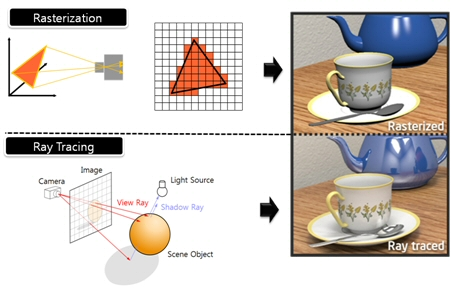
\includegraphics[width=1\textwidth]{images/rasterization_vs_ray_tracing.jpg}
	\caption{Rasterizzazione vs Ray tracing}
	Fonte: \cite{rasterization_vs_ray_tracing}
\end{figure}

\newpage
\subsection{Proiezione e volume di visibilità}

La trasformazione da spazio 3D a immagine 2D avviene attraverso il concetto di \textbf{view frustum}, che definisce precisamente quale porzione dello spazio 3D sarà visibile nell'immagine finale.

\subsubsection{Il view frustum}

Il view frustum è un volume tronco-piramidale con vertice nel punto di osservazione della camera (eye point). È delimitato da sei piani:

\begin{itemize}
    \item \textbf{Near plane}: Il piano più vicino alla camera, definisce la distanza minima di rendering
    \item \textbf{Far plane}: Il piano più lontano, oltre il quale gli oggetti non vengono renderizzati
    \item \textbf{Left/Right planes}: Delimitano l'estensione orizzontale del campo visivo
    \item \textbf{Top/Bottom planes}: Definiscono l'estensione verticale del campo visivo
\end{itemize}

Il frustum è caratterizzato da parametri chiave: il \textbf{field of view} (FOV) che determina l'ampiezza angolare della visione, l'\textbf{aspect ratio} che definisce il rapporto larghezza/altezza dell'immagine, e le distanze \textbf{near} e \textbf{far} che stabiliscono l'intervallo di profondità renderizzabile.

\begin{figure}[htbp]
    \centering
    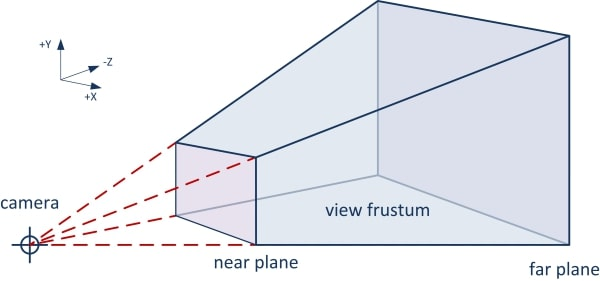
\includegraphics[width=0.9\textwidth]{images/view_frustum.jpg}
    \caption{Rappresentazione del view frustum}
    Fonte: \cite{view_frustum}
\end{figure}

\subsubsection{Tipi di proiezione}

I due tipi principali di proiezione determinano forme diverse del volume di visibilità:

\begin{itemize}
 \item \textbf{Proiezione parallela (o ortografica)}  utilizza raggi paralleli per proiettare gli oggetti sul piano immagine, mantenendo le dimensioni relative costanti indipendentemente dalla distanza. In questo caso, il volume di visibilità non è più un frustum ma diventa un \textbf{parallelepipedo retto} con pareti parallele, poiché non c'è convergenza dei raggi verso un punto di osservazione. Sebbene sia utile per applicazioni CAD e disegno tecnico dove è necessario preservare proporzioni e misure esatte, non è adatta per il rendering 3D realistico poiché non simula la percezione visiva umana.
 \item \textbf{Proiezione prospettica} mantiene invece la forma tronco-piramidale del view frustum, facendo convergere i raggi di proiezione verso il punto di osservazione della camera. Gli oggetti più distanti appaiono più piccoli a causa della convergenza geometrica del frustum, creando un senso naturale di profondità e realismo visivo.
\end{itemize}



\begin{figure}[htbp]
    \centering
    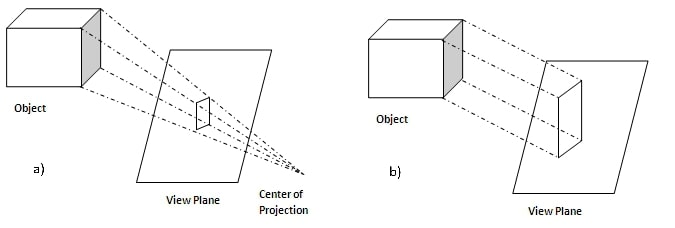
\includegraphics[width=0.8\textwidth]{images/perspective_vs_parallel.jpg}
    \caption{Tipi di proiezione: a) proiezione prospettica b) proiezione parallela}
    Fonte: \cite{projection_types}
\end{figure}
\newpage
 Le rispettive \textbf{matrici di proiezione}, costruite a partire dai parametri del frustum (FOV, aspect ratio, near/far), trasformano le coordinate 3D in coordinate di clip normalizzate, permettendo contemporaneamente la corretta proiezione e l'eliminazione automatica (culling) di geometrie esterne al volume visibile.

\begin{equation}
	P_{ortho} = \begin{pmatrix}
		\frac{2}{r-l} & 0 & 0 & -\frac{r+l}{r-l} \\
		0 & \frac{2}{t-b} & 0 & -\frac{t+b}{t-b} \\
		0 & 0 & -\frac{2}{f-n} & -\frac{f+n}{f-n} \\
		0 & 0 & 0 & 1
	\end{pmatrix}
\end{equation}
\begin{center}
	\textit{Matrice di proiezione ortografica}
\end{center}

\begin{equation}
P_{persp} = \begin{pmatrix}
\frac{2n}{r-l} & 0 & \frac{r+l}{r-l} & 0 \\
0 & \frac{2n}{t-b} & \frac{t+b}{t-b} & 0 \\
0 & 0 & -\frac{f+n}{f-n} & -\frac{2fn}{f-n} \\
0 & 0 & -1 & 0
\end{pmatrix}
\end{equation}
\begin{center}
	\textit{Matrice di proiezione prospettica}
\end{center}

dove $n$ = near plane, $f$ = far plane, $l$ = left, $r$ = right, $t$ = top, $b$ = bottom.
\newline
\noindent La differenza fondamentale risiede nella terza riga: la proiezione prospettica introduce il fattore $-1$ nell'elemento $(4,3)$ che causa la divisione prospettica (trasformazione da coordinate omogenee), mentre la proiezione ortografica mantiene $w = 1$, preservando le proporzioni.

\subsection{Rasterizzazione}

La \textbf{rasterizzazione} è il processo di conversione delle primitive geometriche continue (triangoli, linee, punti) in pixel discreti su una griglia 2D. Rappresenta la fase finale della pipeline di rendering dove le forme geometriche vengono "disegnate" nell'immagine.

Il processo avviene attraverso questi passaggi:

\begin{itemize}
    \item \textbf{Scan conversion}: Determinazione di quali pixel dell'immagine sono coperti da ogni primitiva geometrica
    \item \textbf{Interpolazione}: Calcolo dei valori degli attributi (colore, coordinate texture, normali) per ogni pixel attraverso interpolazione baricentrica nei triangoli
    \item \textbf{Z-buffering}: Gestione della visibilità tramite buffer di profondità per determinare quale superficie è più vicina alla camera
    \item \textbf{Shading}: Applicazione di modelli di illuminazione per calcolare il colore finale di ogni pixel
\end{itemize}

\begin{figure}[htbp]
    \centering
    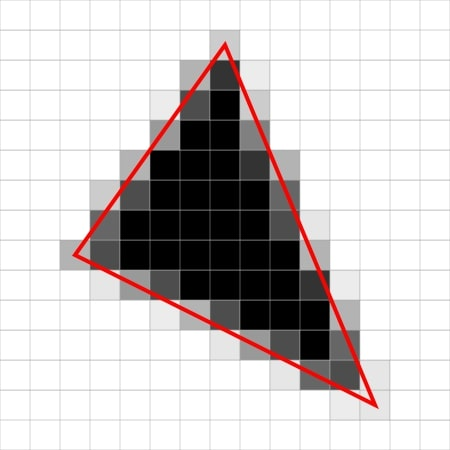
\includegraphics[width=0.5\textwidth]{images/rasterization.jpg}
    \caption{Triangolo 3D rappresentato su uno schermo}
    Fonte: \cite{rasterization}
\end{figure}

\subsection{Considerazioni per GPU moderne}
La rasterizzazione è altamente ottimizzata per le GPU moderne grazie alla sua struttura adatta alle pipeline grafiche tradizionali: processa primitive geometriche in sequenza attraverso stadi fissi. Questo la rende ideale per applicazioni real-time.

\noindent Il ray tracing, pur essendo anch'esso intrinsecamente parallelo (ogni raggio può essere tracciato indipendentemente), richiede strutture dati complesse per l'accelerazione spaziale e accessi di memoria meno prevedibili, risultando tradizionalmente più costoso computazionalmente. Tuttavia, le GPU moderne con unità RT (Ray Tracing) dedicate stanno rendendo il ray tracing sempre più competitivo anche per applicazioni real-time.
\noindent Le GPU moderne sono ottimizzate per parallelismo massivo e throughput elevato. 
Tra le caratteristiche e gli aspetti piu importanti abbiamo:

\begin{itemize}
    \item \textbf{Parallelizzazione}: Migliaia di thread processano simultaneamente diversi pixel o primitive
    \item \textbf{Memory bandwidth}: La velocità di accesso alla memoria è spesso il fattore limitante
    \item \textbf{Coerenza spaziale}: Algoritmi che sfruttano la località spaziale dei dati ottengono prestazioni superiori
\end{itemize}

\noindent Questi principi fondamentali influenzano profondamente la progettazione di tecniche moderne come il 3D Gaussian Splatting, che combina l'efficienza della rasterizzazione con la flessibilità di rappresentazioni alternative alle mesh tradizionali.
\section{Panorama delle rappresentazioni 3D}
\label{sec:panoramica}

\subsubsection{Tecniche tradizionali}
Le rappresentazioni 3D tradizionali si basano principalmente su mesh poligonali e point clouds, che differiscono fondamentalmente nella loro organizzazione dei dati.
\newline\newline
Le \textbf{mesh poligonali} rappresentano dati strutturati: utilizzano triangoli interconnessi per definire superfici continue, dove ogni vertice è connesso ad altri vertici per formare spigoli, che a loro volta si collegano per creare facce triangolari. Questa struttura interconnessa garantisce rappresentazioni geometriche precise e compatibilità con le pipeline di rendering tradizionali, ma richiede maggiore complessità computazionale per la gestione delle connessioni. Inoltre, presentano limitazioni nella gestione di geometrie complesse come capelli, fumo o superfici trasparenti.
\newline\newline
Le \textbf{point clouds}, d'altra parte, rappresentano dati non strutturati: consistono in insiemi discreti di punti nello spazio 3D, ciascuno con posizione e colore associati, ma senza informazioni di connessione tra di essi. Questa caratteristica le rende più semplici da renderizzare dal punto di vista computazionale, poiché ogni punto può essere processato indipendentemente. Sebbene siano efficaci per la cattura di dati da sensori come LiDAR\footnote{Il \textit{LiDAR} (Light Detection and Ranging) è una tecnologia di telerilevamento che misura la distanza dagli oggetti usando impulsi laser. Viene comunemente impiegata per ottenere mappe 3D precise di ambienti, sia in ambito terrestre che aereo.}, soffrono di discontinuità visive e difficoltà nel rendering di superfici smooth.
\begin{figure}[htbp]
    \centering
    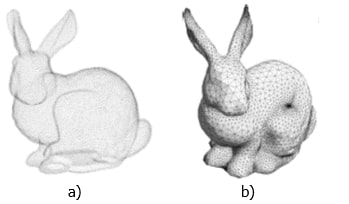
\includegraphics[width=0.9\textwidth]{images/rabbits.jpg}
    \caption{Esempi di modelli 3D: a) point cloud b) mesh poligonale}
    Fonte: \cite{researchgate_bunny}
\end{figure}
Le limitazioni delle rappresentazioni discrete appena citate hanno portato allo sviluppo di approcci volumetrici, che modellano lo spazio 3D come un continuum di proprietà ottiche piuttosto che attraverso elementi geometrici separati.

\subsection{Volume Rendering: verso rappresentazioni continue}

Le limitazioni delle mesh poligonali e dei point clouds hanno portato allo sviluppo di approcci alternativi basati su rappresentazioni volumetriche. Il volume rendering rappresenta un paradigma fondamentale che modella fenomeni difficili da rappresentare con primitive geometriche tradizionali.

\subsubsection{Principi fondamentali}

Come definito da \cite{ikits2004volume}, "Direct volume rendering methods generate images of a 3D volumetric data set without explicitly extracting geometric surfaces from the data". Questa tecnica utilizza un modello ottico per mappare i valori dei dati a proprietà ottiche come colore e opacità.

Il volume rendering assume che il volume sia composto da particelle che simultaneamente emettono e assorbono luce \cite{ikits2004volume}. Durante il rendering, le proprietà ottiche vengono accumulate lungo ogni raggio di vista per formare un'immagine dei dati. Ogni elemento di volume (voxel) corrisponde a una posizione nello spazio dei dati e ha uno o più valori associati.

Il processo di generazione dell'immagine avviene attraverso il campionamento del volume lungo tutti i raggi di vista e l'accumulo delle proprietà ottiche risultanti \cite{ikits2004volume}. Per il modello di emissione-assorbimento, il colore e l'opacità accumulati vengono calcolati iterativamente, ordinando i campioni lungo il raggio di vista.

\begin{figure}[htbp]
    \centering
    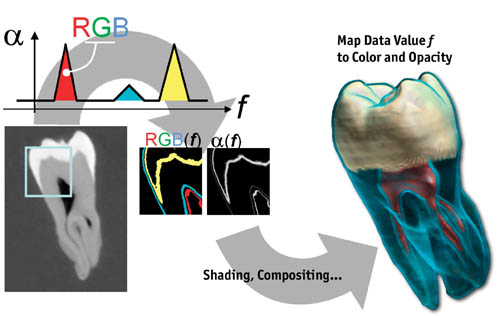
\includegraphics[width=0.9\textwidth]{images/volume_rendering_process.jpg}
    \caption{Il processo del volume rendering}
    Fonte: \cite{volume_rendering_process}
\end{figure}

\subsubsection{Fenomeni volumetrici}

Molti effetti visivi sono di natura volumetrica \cite{ikits2004volume}. Fluidi, nuvole, fuoco, fumo, nebbia e polvere sono difficili da modellare con primitive geometriche. I modelli volumetrici sono meglio adatti per creare tali effetti, poiché assumono che la luce venga emessa, assorbita e diffusa da un gran numero di particelle nel volume.

\subsubsection{Applicazioni scientifiche e ingegneristiche}

Oltre alla modellazione di fenomeni volumetrici, il volume rendering è essenziale per applicazioni scientifiche e ingegneristiche che richiedono la visualizzazione di dataset tridimensionali \cite{ikits2004volume}. Gli esempi includono:

\begin{itemize}
    \item \textbf{Imaging medico}: visualizzazione di dati acquisiti da dispositivi di imaging medicale
    \item \textbf{Simulazioni fluidodinamiche}: visualizzazione di risultati da simulazioni computazionali
    \item \textbf{Esplorazione scientifica}: analisi interattiva di dati volumetrici complessi
\end{itemize}

Gli utenti di applicazioni di volume rendering interattivo si affidano alle prestazioni degli acceleratori grafici moderni per un'esplorazione efficiente dei dati e la scoperta di caratteristiche.

\subsubsection{Limitazioni tecniche}

Il volume rendering presenta diverse sfide computazionali significative \cite{ikits2004volume}:

\begin{itemize}
    \item \textbf{Richieste hardware elevate}: necessita di computer molto potenti per ottenere risultati in tempo reale
    \item \textbf{Velocità di rendering limitata}: il processo è più lento rispetto al rendering di oggetti solidi tradizionali
    \item \textbf{Consumo di memoria}: i dati volumetrici richiedono grandi quantità di memoria per scene dettagliate
    \item \textbf{Complessità algoritmica}: gli algoritmi necessari sono matematicamente e computazionalmente complessi
\end{itemize}

\subsubsection{Evoluzione verso tecniche moderne}

Il volume rendering ha costituito la base teorica per lo sviluppo di tecniche moderne di \textbf{novel view synthesis}, cioè la generazione di immagini realistiche di una scena da angolazioni o posizioni di osservazione non presenti nel set originale di immagini. Le tecniche texture-based descritte da \cite{ikits2004volume} hanno dimostrato come sia possibile combinare facilmente algoritmi poligonali con volume rendering, richiedendo solo pochi pass di rendering e offrendo un alto livello di interattività senza sacrificare la qualità del rendering.
\newline
\newline
Questa flessibilità ha aperto la strada a rappresentazioni ibride che combinano i vantaggi del volume rendering con l'efficienza di primitive esplicite. Prima i Neural Radiance Fields (NeRF), poi il 3D Gaussian Splatting, possono essere visti come un'evoluzione naturale di questi concetti, mantenendo la capacità di rappresentare fenomeni volumetrici complessi.
\newline
\newline
L'eredità del volume rendering è particolarmente evidente nella gestione delle proprietà ottiche e nell'accumulo lungo i raggi di vista, principi che rimangono centrali nelle tecniche moderne di neural rendering e rappresentazioni gaussiane.

\subsubsection{Neural Radiance Fields (NeRF)}

L'evoluzione del volume rendering verso approcci basati su machine learning ha trovato la sua espressione più innovativa nei Neural Radiance Fields (NeRF), introdotti da \cite{mildenhall2020nerf}. Questa tecnica rappresenta un salto paradigmatico nella rappresentazione di scene 3D, utilizzando reti neurali per codificare implicitamente volumi continui attraverso funzioni differenziabili.

\begin{figure}[htbp]
	\centering
	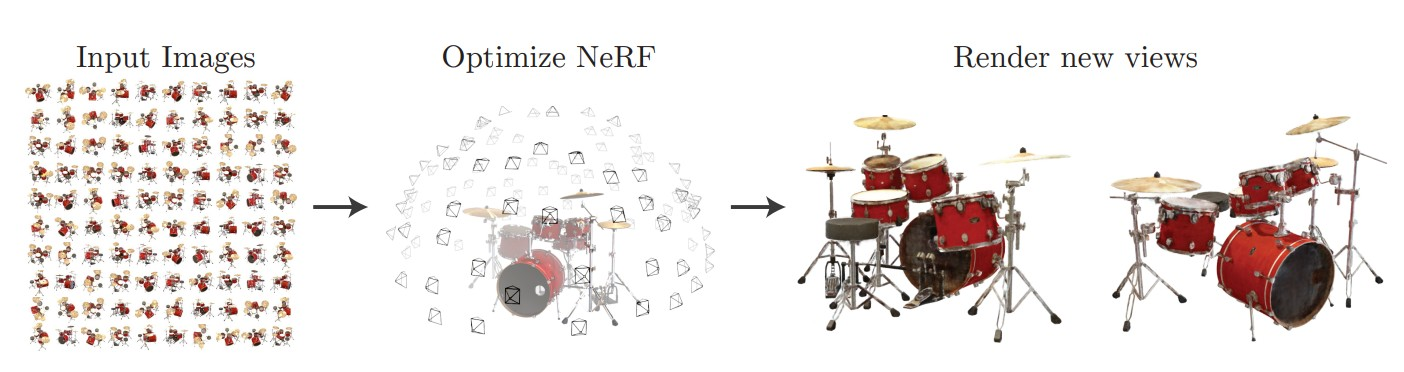
\includegraphics[width=0.9\textwidth]{images/5d_optimization.jpg}
	\caption{Ottimizzazione di una rappresentazione 5D continua}
	Fonte: \cite{5d_optimization}
\end{figure}

\paragraph{Rappresentazione 5D continua}
NeRF modella una scena statica come una funzione continua 5D che mappa coordinate spaziali 3D $(x, y, z)$ e direzioni di vista 2D $(\theta, \phi)$ a proprietà ottiche: densità volumetrica $\sigma$ e colore emesso dipendente dalla vista $(r, g, b)$. Questa rappresentazione viene approssimata attraverso una rete neurale Multi-Layer Perceptron (MLP)\footnote{Un \textit{Multi-Layer Perceptron} (MLP) è una rete neurale artificiale composta da più strati di neuroni completamente connessi. È in grado di apprendere relazioni non lineari tra input e output attraverso l'addestramento supervisionato.} completamente connessa $F_\Theta : (x, d) \rightarrow (c, \sigma)$, dove $\Theta$ rappresenta i pesi ottimizzabili della rete.

L'architettura impone vincoli di consistenza multi-vista: la densità volumetrica $\sigma$ dipende esclusivamente dalla posizione spaziale $x$, mentre il colore RGB $c$ può variare in funzione sia della posizione che della direzione di vista $d$. Questa separazione consente di rappresentare effetti non-Lambertiani\footnote{Gli \textit{effetti non-Lambertiani} sono fenomeni ottici in cui la luce riflessa da una superficie varia in base all’angolo di osservazione, come accade con i riflessi speculari, le superfici lucide o traslucide. Diversamente dai materiali Lambertiani, che riflettono la luce in modo uniforme, questi effetti dipendono dalla direzione della visuale.} come riflessi speculari e variazioni di colore dipendenti dall'angolo di osservazione.

\paragraph{Rendering volumetrico differenziabile}
Il processo di rendering utilizza principi classici del volume rendering per accumulare colore e opacità lungo raggi camera. Per un raggio $r(t) = o + td$ con limiti near e far $t_n$ e $t_f$, il colore atteso $C(r)$ viene calcolato attraverso l'integrale:

\begin{equation}
	C(r) = \int_{t_n}^{t_f} T(t)\sigma(r(t))c(r(t), d)dt
\end{equation}

dove $T(t) = \exp(-\int_{t_n}^{t} \sigma(r(s))ds)$ rappresenta la trasmittanza accumulata lungo il raggio. L'integrale viene approssimato numericamente attraverso campionamento stratificato, evitando le limitazioni di risoluzione delle griglie voxel discrete.

\paragraph{Innovazioni tecniche}
NeRF introduce due miglioramenti fondamentali per ottenere risultati di qualità elevata:

\begin{itemize}
\item \textbf{Positional Encoding}: Le coordinate di input vengono mappate in uno spazio dimensionale superiore utilizzando funzioni sinusoidali ad alta frequenza. Questo approccio, ispirato ai Transformer\footnote{I \textit{Transformer} sono un'architettura di rete neurale basata sull'attenzione, progettata per elaborare sequenze di dati (come testo o tempo) senza l'uso di strutture ricorrenti. Introdotti nel contesto del Natural Language Processing, usano il \textit{positional encoding} per incorporare informazioni sulla posizione degli elementi nella sequenza.}, consente alla rete di rappresentare dettagli ad alta frequenza che altrimenti verrebbero smussati dalla tendenza delle reti neurali verso funzioni a bassa frequenza.

\item \textbf{Campionamento gerarchico}: Il sistema utilizza due reti distinte ("coarse" e "fine") per allocare efficientemente i punti di campionamento. La rete coarse fornisce una distribuzione di probabilità che guida un campionamento più informato per la rete fine, concentrando le risorse computazionali nelle regioni più rilevanti del volume.
\end{itemize}

\paragraph{Vantaggi e limitazioni}
I Neural Radiance Fields hanno dimostrato capacità superiori nella sintesi di nuove viste rispetto ai metodi precedenti, particolarmente nella rappresentazione di scene complesse con geometrie intricate e materiali non-Lambertiani. La rappresentazione continua elimina gli artefatti di discretizzazione tipici delle griglie voxel, mentre i requisiti di memoria sono significativamente ridotti rispetto agli approcci volumetrici tradizionali.

Tuttavia, NeRF presenta limitazioni significative in termini di efficienza computazionale. Il training richiede tipicamente 1-2 giorni su GPU high-end per singole scene, mentre il rendering è computazionalmente intensivo, richiedendo centinaia di milioni di query alla rete per singola immagine. Questa inefficienza limita l'applicabilità in contesti real-time o interattivi.

\paragraph{Impatto e eredità}
NeRF ha stabilito i fondamenti teorici per una nuova generazione di tecniche di novel view synthesis, influenzando lo sviluppo di rappresentazioni ibride che combinano i vantaggi del rendering volumetrico con primitive più efficienti. I principi di rappresentazione continua, rendering differenziabile e ottimizzazione basata su immagini costituiscono l'eredità concettuale che ha ispirato successive innovazioni come il 3D Gaussian Splatting.
\section{Fondamenti teorici del Gaussian Splatting}
\subsection{Rappresentazione 3D basata su gaussiane}

Il 3D Gaussian Splatting introduce un paradigma innovativo per la rappresentazione di scene tridimensionali, utilizzando primitive gaussiane 3D come elementi fondamentali in alternativa alle tradizionali mesh poligonali o ai Neural Radiance Fields impliciti.

Mentre le metodologie consolidate si basano su mesh poligonali progettate da artisti 3D o su nuvole di punti generate tramite tecniche di fotogrammetria classica, il 3D Gaussian Splatting adotta un approccio radicalmente diverso. Il dataset di partenza consiste in foto o video acquisiti direttamente da oggetti o scene del mondo reale, oppure in scene sintetiche generate artificialmente tramite motori grafici o dataset simulati. Questi dati vengono successivamente elaborati attraverso algoritmi specializzati per generare una rappresentazione tridimensionale fotorealistica basata su primitive gaussiane.

Questa metodologia offre il vantaggio significativo di catturare scene complesse del mondo reale con un livello di fedeltà visiva superiore, preservando dettagli come riflessi accurati ed effetti anisotropi direzionali che risultano difficili da riprodurre con le tecniche tradizionali di computer grafica.

\paragraph{Il concetto di "Splats" nella computer grafica
}
Per comprendere meglio il concetto di primitiva gaussiana, è utile introdurre il termine "splats", una tecnica di computer grafica introdotta nel 2001 che ha trovato diverse applicazioni nel rendering 3D. Nel contesto del rendering di point cloud, gli splats hanno dimostrato la loro efficacia nel migliorare significativamente la qualità visiva delle rappresentazioni basate su punti.
Quando si renderizza una point cloud tradizionale, ogni punto viene semplicemente colorato con il proprio colore specifico. Tuttavia, la tecnica degli splats introduce un approccio più sofisticato: durante il processo di shading di ciascun punto primitivo sullo schermo, il sistema tiene conto anche del colore dei punti posizionati dietro di esso. Questo permette di renderizzare "splats" che fondono i punti in modo armonioso dal punto di vista visivo, creando una rappresentazione molto più fluida e fotorealistica della point cloud.
La differenza visiva tra una point cloud tradizionale e una renderizzata con splats è particolarmente evidente: mentre la prima appare spesso frammentata e discontinua, la seconda presenta superfici continue e naturali che risultano molto più accattivanti anche per chi non ha familiarità con il rendering 3D. Questo principio di blending intelligente tra primitive adiacenti costituisce la base concettuale su cui si fonda il 3D Gaussian Splatting.


\begin{figure}[htbp]
	\centering
	
	\begin{subfigure}{0.45\textwidth}
		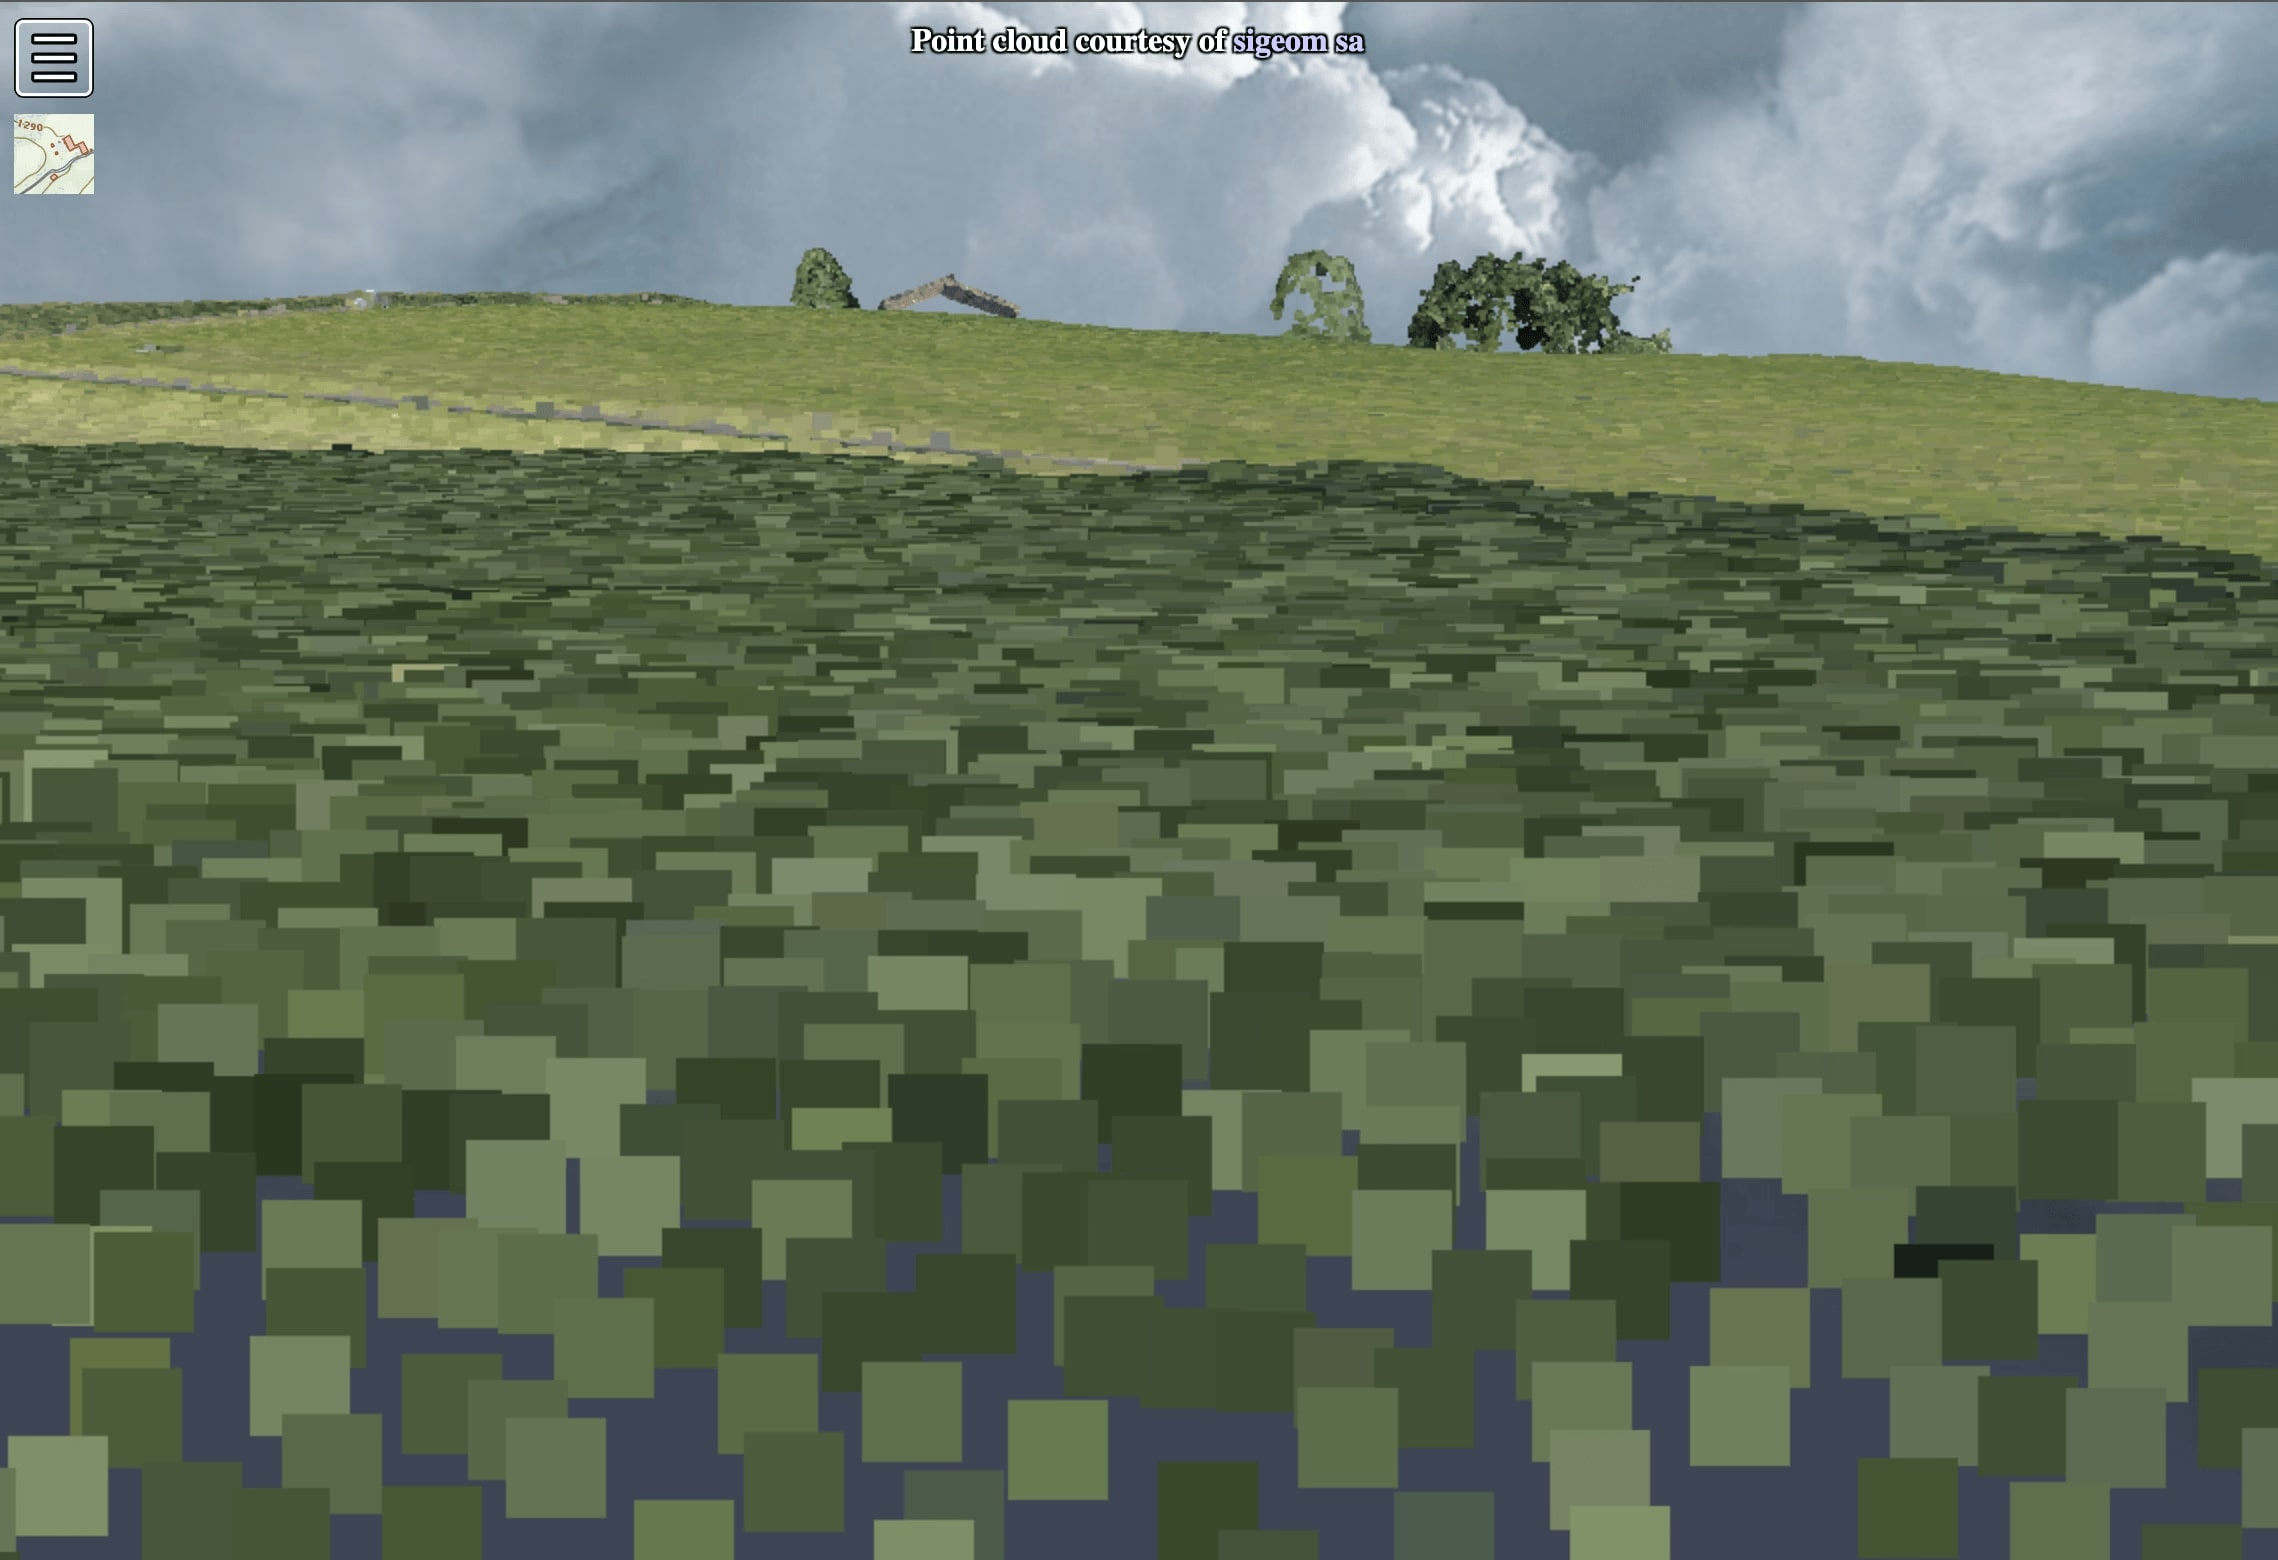
\includegraphics[width=\linewidth,  trim={80 40 80 40}, clip]{images/points.jpg}
		\caption{Point cloud tradizionale} 
		\label{fig:point_cloud_traditional}
	\end{subfigure}
	\hfill
	\begin{subfigure}{0.45\textwidth}
		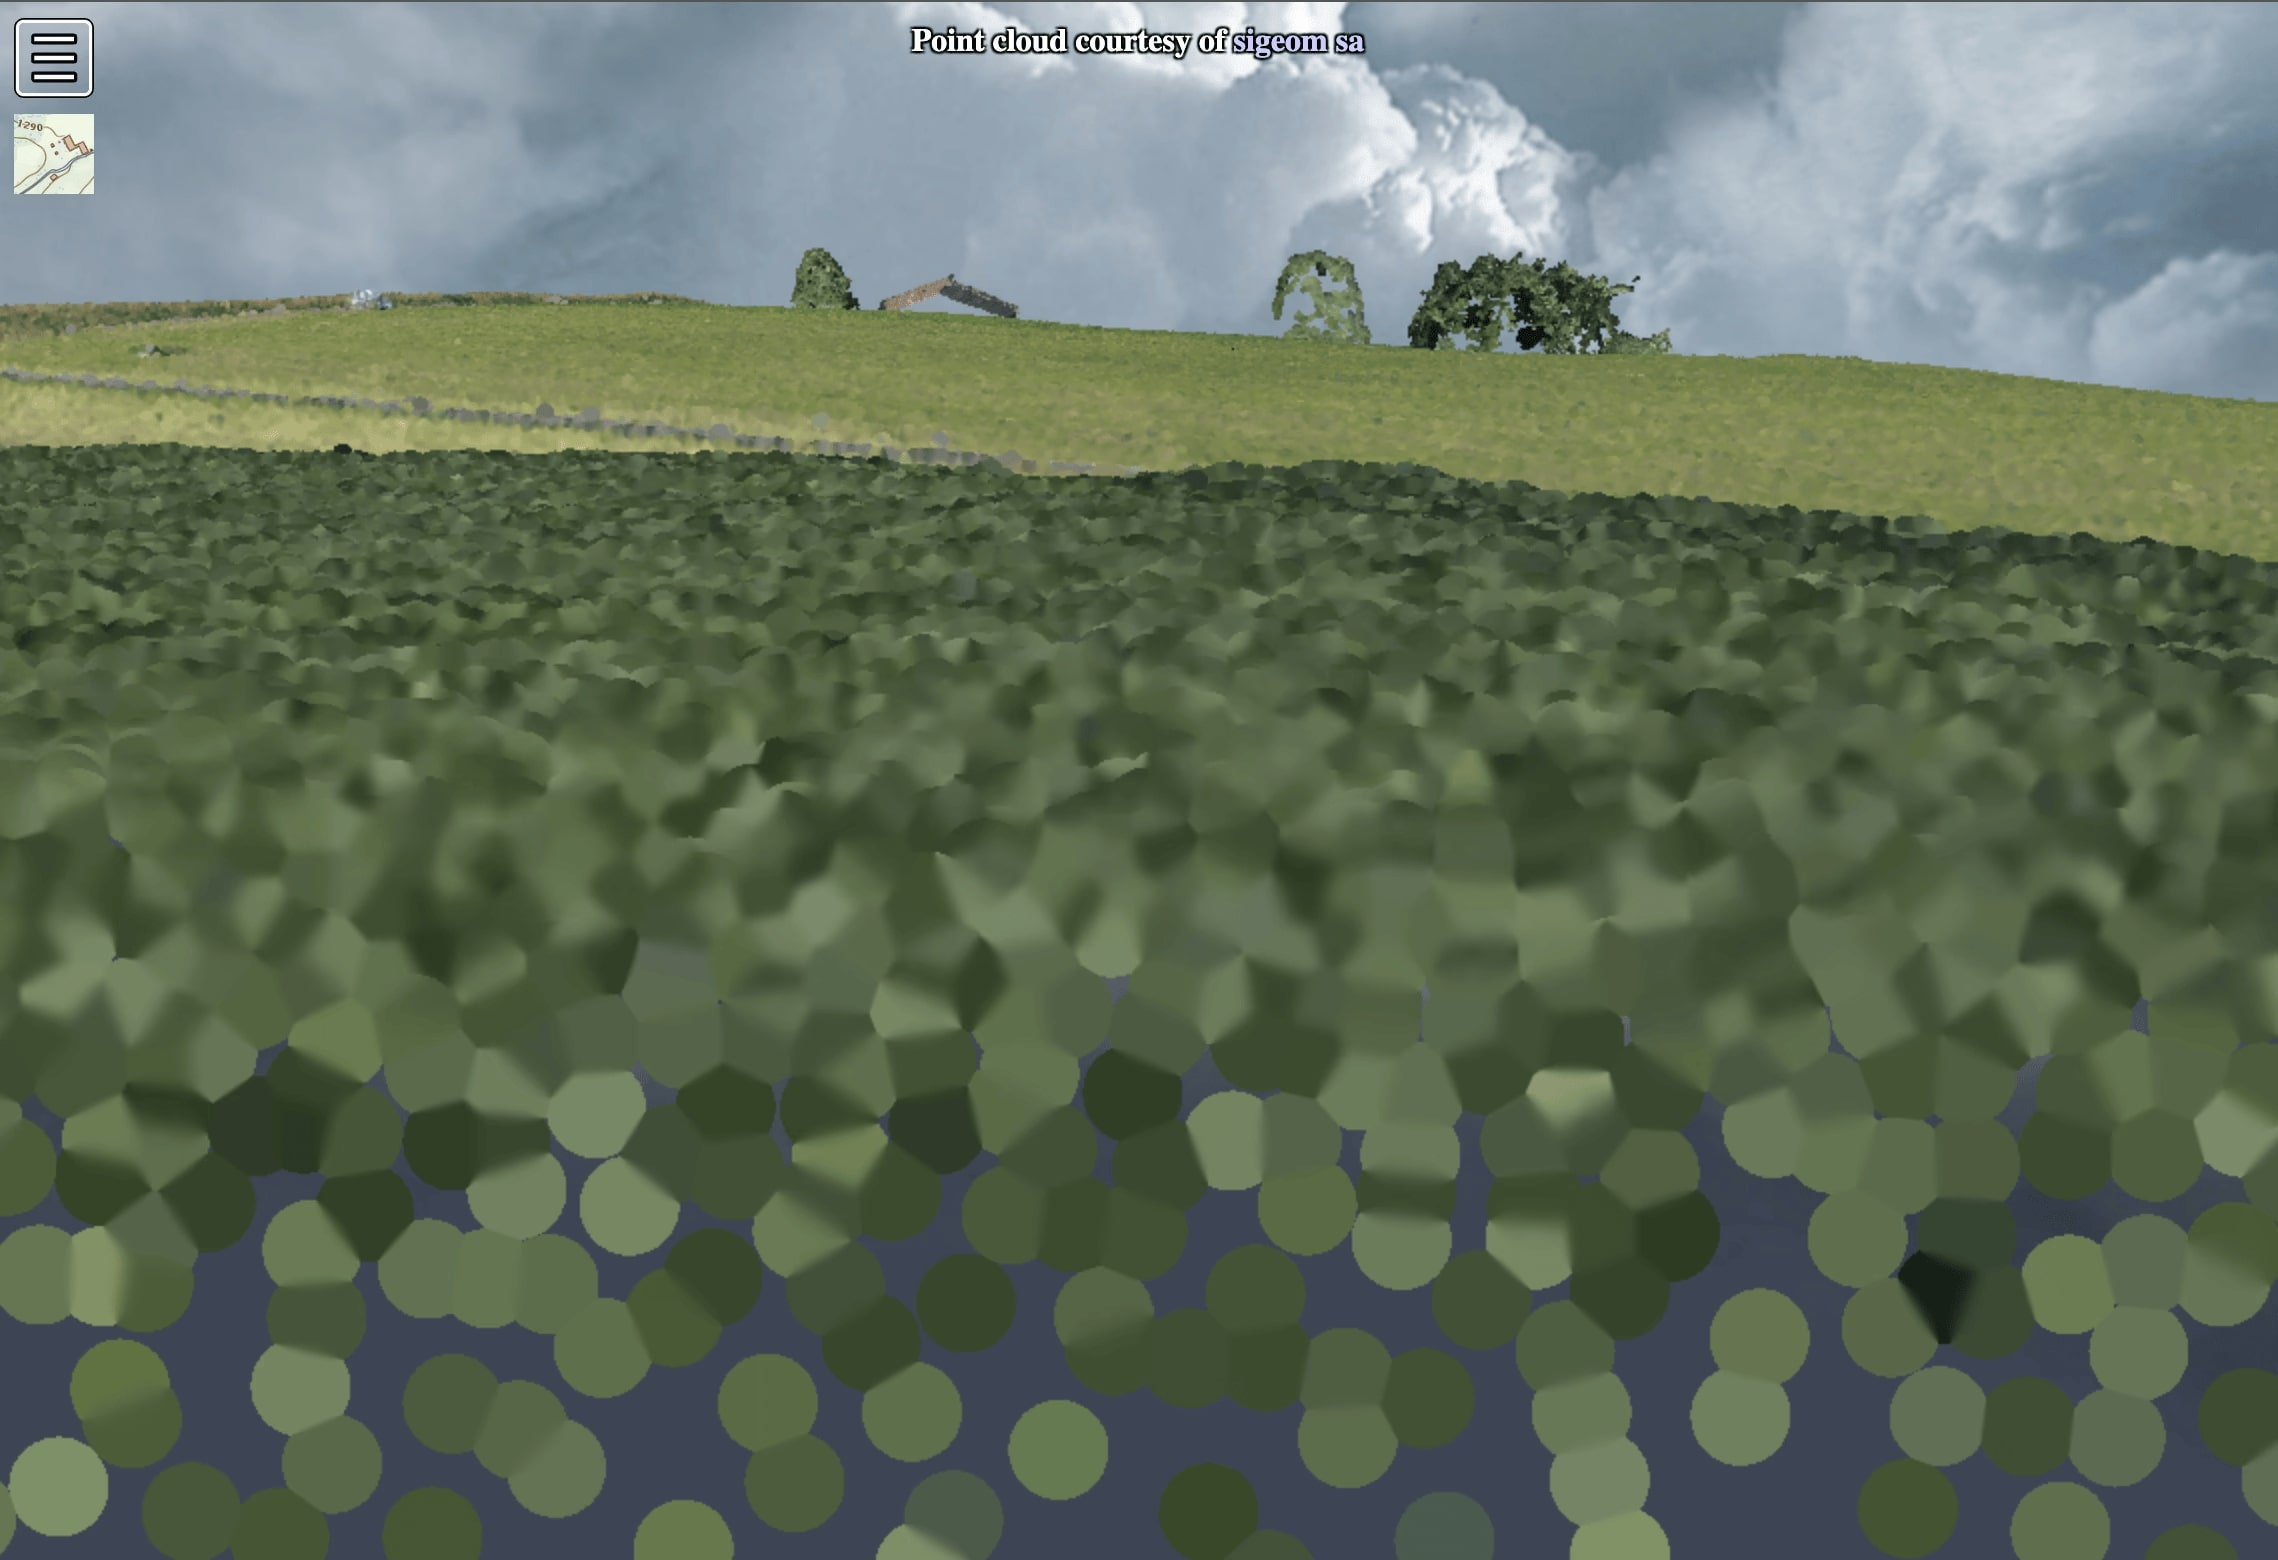
\includegraphics[width=\linewidth, trim={80 40 80 40}, clip]{images/splats.jpg}
		\caption{Point cloud con splatting}  
		\label{fig:point_cloud_with_splatting}
	\end{subfigure}
	\caption{Confronto tra point cloud tradizionale e splatting} \cite{point_cloud_traditional}, \cite{point_cloud_with_splatting}
	\label{fig:comparison_point_clouds}
	,
\end{figure}


\paragraph{Primitive gaussiane come building blocks
}
Una \textbf{gaussiana 3D} può essere concettualizzata come un ellissoide tridimensionale che rappresenta un "pennellata" nello spazio 3D con proprietà variabili. A differenza dei triangoli utilizzati nelle mesh tradizionali o dei punti discreti delle point cloud, le gaussiane offrono una rappresentazione continua e flessibile che può adattarsi a diverse forme geometriche.
\newline
\newline
Ogni gaussiana 3D è definita da un insieme di parametri fondamentali:
\begin{itemize}
\item \textbf{Posizione media $\mu$}: Le coordinate XYZ del centro della gaussiana nello spazio tridimensionale
\item \textbf{Matrice di covarianza $\Sigma$}: Una matrice 3×3 che definisce la forma, le dimensioni e l'orientamento dell'ellissoide gaussiano
\item \textbf{Opacità $\alpha$}: Il grado di trasparenza della primitiva, cruciale per il blending tra gaussiane sovrapposte
\item \textbf{Colore dipendente dalla vista}: Valori RGB che possono essere view-dependent attraverso l'uso di armoniche sferiche
\end{itemize}

\newpage
La funzione gaussiana 3D è espressa come:

\begin{equation}
G(x) = \exp\left(-\frac{1}{2}(x-\mu)^T\Sigma^{-1}(x-\mu)\right)
\end{equation}

\paragraph{Vantaggi della rappresentazione gaussiana}\mbox{}\\
La scelta delle gaussiane come primitive presenta diversi vantaggi significativi:

\begin{itemize}
    \item \textbf{Compattezza rappresentativa}: Scene complesse possono essere rappresentate con 1-5 milioni di gaussiane, mentre point cloud equivalenti potrebbero richiedere decine di milioni o miliardi di punti per la stessa qualità visiva.

    \item \textbf{Fotorealismo}: Le gaussiane permettono di ottenere risultati visivi estremamente realistici, catturando dettagli sottili di illuminazione, ombre e riflessi che spesso mancano in altre rappresentazioni 3D.
    
    \item \textbf{Rappresentazione di geometrie complesse}: A differenza delle mesh che faticano con superfici non-manifold\footnote{Una superficie è \emph{manifold} se l'intorno di ogni punto è topologicamente equivalente a un disco e ogni spigolo è condiviso da esattamente due facce. Esempi di geometrie \emph{non-manifold} includono: spigoli condivisi da tre o più facce, vertici \emph{bow-tie}, giunzioni a T e lamine di spessore nullo.} o topologie complesse, le gaussiane possono rappresentare naturalmente geometrie intricate, dettagli fini e strutture organiche.
    
    \item \textbf{Proprietà anisotrope}: Le gaussiane possono avere valori diversi quando osservate da direzioni diverse. Questa anisotropia, implementata attraverso armoniche sferiche, consente sia di rappresentare strutture geometriche sottili (come fili d'erba o capelli) che di catturare effetti ottici realistici come riflessi che cambiano con il punto di vista.
\end{itemize}
\begin{figure}[htbp]
    \centering
    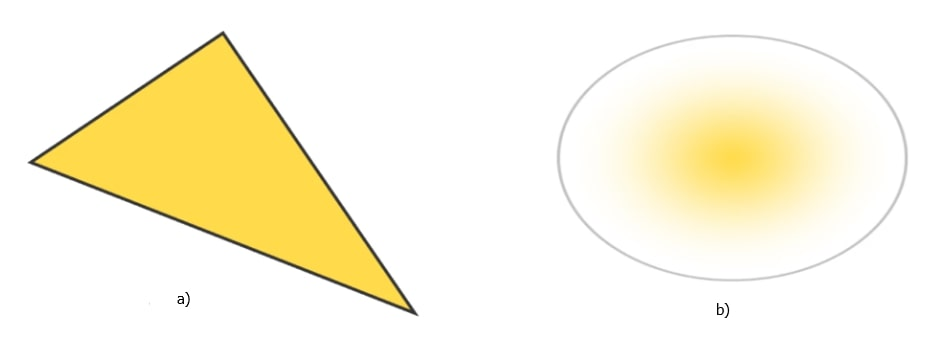
\includegraphics[width=0.9\textwidth]{images/gaussiana_vs_triangle.jpg}
    \caption{Due diverse primitive: a) triangolo b) gaussiana}
    \label{fig:gaussian_and_triangle_mesh}
\end{figure}


\subsection{Pipeline di training}
Il processo di creazione di una rappresentazione Gaussian Splatting segue una pipeline strutturata che trasforma immagini o video di input in un insieme ottimizzato di gaussiane 3D.
La pipeline è così strutturata:
\begin{enumerate}
    \item \textbf{Structure from Motion (SfM)}: Il processo inizia con l'analisi delle immagini di input utilizzando tecniche di Structure from Motion\footnote{La \textit{Structure from Motion} (SfM) è una tecnica di visione artificiale che ricostruisce la geometria tridimensionale di una scena e le traiettorie della camera a partire da immagini bidimensionali multiple, sfruttando la parallasse tra viste. Per un approfondimento si rimanda alla sezione 1.4.}. È necessario che le immagini abbiano sovrapposizione adeguata e coprano la scena da angolazioni diverse. Questa fase genera una point cloud sparsa e stima le pose delle camere, fornendo la struttura geometrica iniziale della scena.

    \item \textbf{Inizializzazione delle gaussiane}: Ogni punto della point cloud sparsa viene successivamente convertito in una gaussiana 3D. Ogni gaussiana viene inizializzata con la posizione del punto corrispondente, il colore derivato dalle osservazioni delle camere, e parametri geometrici di default (covarianza isotropa e opacità iniziale).
    
    \item \textbf{Ottimizzazione differenziabile}: Il cuore del training consiste nell'ottimizzazione dei parametri gaussiani attraverso \textbf{Stochastic Gradient Descent (SGD)}. SGD è un algoritmo di ottimizzazione che trova iterativamente i parametri del modello che minimizzano la differenza tra risultati predetti e target reali.\newline
    A ogni iterazione, il processo seleziona una singola immagine dal dataset di training e confronta l'immagine renderizzata dalla rappresentazione gaussiana corrente con questa immagine target, calcolando una loss function $\mathcal{L}$ che combina:
        \begin{itemize}
            \item \textbf{$\mathcal{L}_1$ (L1 loss)}: misura la differenza assoluta tra pixel corrispondenti delle immagini
            \item \textbf{$\mathcal{L}_{\text{D-SSIM}}$ (Structural Dissimilarity)}: valuta la similarità strutturale e percettiva tra le immagini, catturando differenze che l'occhio umano noterebbe meglio della semplice differenza di colore
        \end{itemize}
        La funzione di loss combinata è definita come:
        \begin{equation}
            \mathcal{L} = (1-\lambda)\mathcal{L}_1 + \lambda \mathcal{L}_{\text{D-SSIM}}
        \end{equation}
        
    dove $\lambda$ è un iperparametro (tipicamente 0.2) che bilancia l'importanza tra accuratezza del colore e similarità strutturale: $\mathcal{L}_1$ garantisce l'accuratezza dei colori di base, che è più critica per la convergenza dell'ottimizzazione rispetto ai dettagli strutturali catturati da D-SSIM.
    L'algoritmo varia i parametri della gaussiane (posizione, colore, forma, dimensione e trasparenza) basandosi su questa funzione di loss.
    
    \item \textbf{Controllo adattivo della densità}: Durante il training, il sistema implementa strategie di densificazione e pruning per ottimizzare il numero e la distribuzione delle gaussiane. Quando una regione è sotto-rappresentata, le gaussiane vengono duplicate (cloning) o suddivise (splitting) per catturare dettagli fini. Di contro, gaussiane con opacità molto bassa vengono rimosse per mantenere efficienza computazionale.
\end{enumerate}

\begin{figure}[htbp]
    \centering
    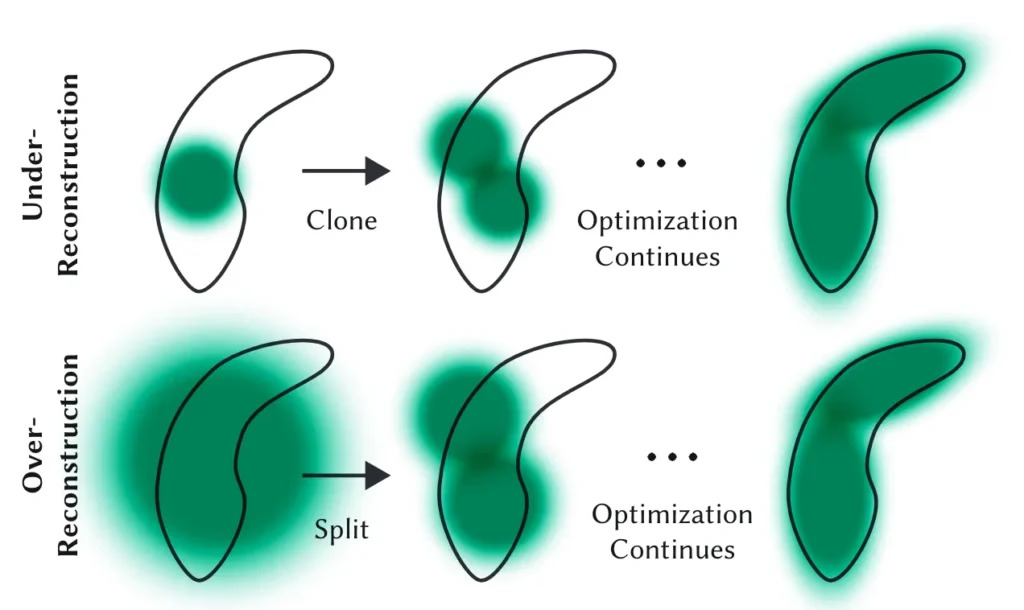
\includegraphics[width=0.9\textwidth]{images/densification.jpg}
    \caption{Densificazione della gaussiane cloning e splitting}
    \label{fig:densification}
\end{figure}

\paragraph{Rasterizzazione differenziabile}
Perché sia possibile l'ottimizzazione descritta sopra, è fondamentale che il processo di rendering sia differenziabile - ovvero che permetta di calcolare come una piccola modifica ai parametri delle gaussiane influenzi il risultato finale dell'immagine renderizzata. Questo collegamento è realizzato attraverso il processo di rasterizzazione differenziabile.
Il rendering delle gaussiane 3D avviene attraverso un processo di rasterizzazione tile-based ottimizzato per hardware GPU, composto dai seguenti passaggi:

\begin{enumerate}
    \item \textbf{Proiezione e ordinamento}: Le gaussiane 3D vengono proiettate sul piano immagine 2D dalla prospettiva della camera. Successivamente, il sistema suddivide lo schermo in tile di 16×16 pixel e raggruppa le gaussiane per tile in base alla loro posizione proiettata.
    \item \textbf{Sorting per depth}: All'interno di ogni tile, le gaussiane vengono ordinate per profondità (distanza dal piano dell'immagine), permettendo un corretto alpha-blending front-to-back durante il rendering.
    \item \textbf{Alpha-blending ottimizzato}: Per ogni pixel, il sistema esegue alpha-blending\footnote{L'\textit{alpha-blending} è una tecnica di compositing che combina più colori in base alla loro opacità (canale alpha), producendo effetti di trasparenza graduata.} delle gaussiane ordinate, combinando i loro contributi di colore e opacità. Questo processo genera gradienti smooth e permette la rappresentazione di superfici continue e effetti di trasparenza complessi.
\end{enumerate}

Il processo di rasterizzazione è completamente differenziabile, permettendo la propagazione dei gradienti attraverso l'intera pipeline di rendering per l'ottimizzazione end-to-end.

\paragraph{View-dependent rendering}
Una caratteristica distintiva del Gaussian Splatting è la capacità di rappresentare effetti ottici che dipendono dalla direzione di osservazione. Questo viene ottenuto attraverso l'uso di \textbf{armoniche sferiche (Spherical Harmonics, SH).}
\newline
\newline
Ogni gaussiana memorizza coefficienti di armoniche sferiche che modulano il colore in base alla direzione di vista. Questa rappresentazione permette di catturare fenomeni come:

\begin{itemize}
    \item Riflessi speculari su superfici lucide
    \item Variazioni di colore dovute a materiali anisotropi
    \item Effetti di illuminazione complessi
    \item Proprietà ottiche direzionali dei materiali
\end{itemize}

\subsection{Strutture dati per gaussiane 3D}

Ogni gaussiana 3D richiede la memorizzazione di diversi parametri:
\begin{itemize}
    \item \textbf{Posizione}: 3 coordinate float (12 bytes)
    \item \textbf{Rotazione}: 4 componenti quaternion (16 bytes)
    \item \textbf{Scala}: 3 valori per gli assi dell'ellissoide (12 bytes)
    \item \textbf{Opacità}: 1 valore alpha (4 bytes)
    \item \textbf{Coefficienti SH}: Variabili in base al grado delle armoniche sferiche (tipicamente 48-192 bytes)
\end{itemize}

Una singola gaussiana richiede quindi circa 92-236 bytes, e con rappresentazioni contenenti 1-5 milioni di gaussiane, i dataset possono facilmente raggiungere centinaia di MB o diversi GB.

\subsubsection{Considerazioni per applicazioni web}

Due fattori critici influenzano l'implementazione web:

\begin{itemize}
\item \textbf{Tempi di caricamento}: La dimensione dei dataset può variare significativamente. Scene semplici possono richiedere 50-100 MB, mentre scene complesse possono superare i 2-6 GB. Per applicazioni web, tempi di download prolungati compromettono l'esperienza utente.

\item \textbf{Performance di rendering}: Le prestazioni sono misurate in FPS (frames per second), con l'obiettivo di mantenere ≥30 FPS per interazioni fluide. La variabilità dell'hardware utente (da dispositivi mobili economici a workstation grafiche) richiede strategie di ottimizzazione adattive.
\end{itemize}
\subsubsection{Formati e ottimizzazioni}
La rappresentazione GSplat, essendo concettualmente simile alle point cloud,
utilizza formati di file che riflettono questa affinità. Il formato più comune-
mente adottato è il PLY (.ply), un formato standard ampiamente utilizzato
per la memorizzazione di dati geometrici 3D. Questo formato si adatta natu-
ralmente alla struttura dei dati gaussiani, permettendo di memorizzare tutti
i parametri essenziali di ogni gaussiana: posizione, matrice di covarianza,
opacità e coefficienti delle armoniche sferiche per il colore view-dependent.
Parallelamente allo sviluppo della tecnologia GSplat, la comunità open sour-
ce sta creando formati specializzati come .splat e .ksplat (versione compressa), ottimizzati specificamente per le caratteristiche uniche delle gaussiane 3D. Questo è un campo in rapida evoluzione, con nuovi formati che
emergono continuamente per rispondere alle esigenze specifiche di diverse
applicazioni.
Tuttavia, per applicazioni web potrebbero essere necessarie una o più delle seguenti ottimizzazioni:

\begin{itemize}
    \item \textbf{Compressione}: Tecniche di quantizzazione per ridurre la precisione floating-point mantenendo qualità visiva
    \item \textbf{Streaming progressivo}: Caricamento incrementale per visualizzazione immediata con raffinamento graduale
    \item \textbf{Level-of-Detail (LOD)}: Rappresentazioni multiple a diverse risoluzioni per adattarsi alle capacità hardware
    \item \textbf{Culling spaziale}: Eliminazione di gaussiane non visibili per ridurre il carico computazionale
\end{itemize}

Queste considerazioni sono fondamentali per lo sviluppo di piattaforme accessibili che rendano il 3D Gaussian Splatting fruibile su una vasta gamma di dispositivi e connessioni di rete.
\subsection{Posizionamento nel panorama delle tecniche attuali}
Il 3D Gaussian Splatting si posiziona come soluzione ibrida che combina vantaggi di diverse famiglie di tecniche di rappresentazione 3D.
\newline
\newline
\textbf{Rispetto alle mesh tradizionali}: Mentre le mesh eccellono nella rappresentazione di superfici ben definite e sono ottimizzate per pipeline di rendering consolidate, il Gaussian Splatting offre maggiore flessibilità per fenomeni volumetrici e materiali trasparenti, pur mantenendo efficienza di rendering comparabile.
\newline
\newline
\textbf{Rispetto ai Neural Radiance Fields}: NeRF utilizza reti neurali per rappresentare implicitamente radiance field volumetrici, ottenendo alta qualità visiva ma richiedendo tempi di rendering significativamente più lunghi (secondi per frame). Il Gaussian Splatting raggiunge qualità visiva comparabile con velocità di rendering real-time ($\geq$ 30 FPS), eliminando la necessità di query neurali durante il rendering.
\newline
\newline
\textbf{Rispetto alle point cloud}: Condividendo la natura di dati non strutturati, il Gaussian Splatting supera le limitazioni delle point cloud tradizionali attraverso primitive più espressive (ellissoidi vs punti) e capacità di rappresentare continuità spaziale e effetti ottici complessi.

\paragraph{Innovazioni architetturali}
Il successo del Gaussian Splatting deriva da diverse innovazioni tecniche chiave:
\begin{itemize}
    \item \textbf{Rasterizzazione tile-based}: L'approccio di suddivisione in tile riduce significativamente la complessità computazionale del sorting e dell'alpha-blending, rendendo possibile il rendering real-time di milioni di gaussiane.
    \item \textbf{Differenziabilità end-to-end}: L'intera pipeline, dalla rappresentazione 3D al rendering 2D, è completamente differenziabile, permettendo ottimizzazione diretta tramite gradient descent senza approssimazioni.
    \item \textbf{Controllo adattivo automatico}: Il sistema di densificazione e pruning automatico permette di bilanciare dinamicamente qualità visiva e efficienza computazionale durante il training.
\end{itemize}
Queste caratteristiche posizionano il 3D Gaussian Splatting come tecnica particolarmente adatta per applicazioni che richiedono il bilanciamento di alta qualità visiva, efficienza computazionale e tempi di training ragionevoli, rendendolo ideale per lo sviluppo di piattaforme accessibili come quella proposta in questo lavoro.

\section{Structure from Motion e COLMAP: prerequisiti per 3D Gaussian Splatting}

Prima di fornire una panoramica sugli algoritmi coinvolti nella realizzazione di questo specifico progetto, è fondamentale comprendere il processo di preprocessing che rende possibile l'applicazione di queste tecniche. Tutti gli algoritmi di 3DGS, indipendentemente dalle loro specifiche implementazioni, condividono un requisito comune: la necessità di una nuvola di punti 3D iniziale e delle pose precise delle camere per ogni immagine di input. Questi dati vengono tipicamente generati attraverso tecniche di Structure from Motion (SfM), con COLMAP che rappresenta lo standard de facto per questa fase di preprocessing.

\subsection{Structure from Motion: ricostruzione 3D da immagini}

Structure from Motion (SfM) è una famiglia di algoritmi di computer vision che permette di ricostruire la struttura tridimensionale di una scena e le posizioni delle camere a partire da una collezione di immagini bidimensionali non ordinate. Il principio fondamentale si basa sulla geometria epipolare: quando lo stesso punto fisico viene osservato da due o più posizioni differenti, è possibile triangolare la sua posizione nello spazio 3D utilizzando i principi della geometria proiettiva.

Il processo SfM può essere sintetizzato in tre fasi principali. Inizialmente, vengono estratti punti caratteristici (feature) da ogni immagine utilizzando algoritmi come SIFT, SURF o ORB. Successivamente, questi punti vengono messi in corrispondenza tra immagini diverse per identificare lo stesso punto fisico osservato da angolazioni multiple. Infine, utilizzando queste corrispondenze, viene ricostruita simultaneamente la struttura 3D della scena e le pose delle camere attraverso tecniche di ottimizzazione non lineare.

\noindent L'output di un algoritmo SfM consiste tipicamente in una nuvola di punti 3D sparsa che rappresenta i punti caratteristici della scena, le pose delle camere (posizione e orientamento) per ogni immagine, e i parametri intrinseci delle camere (lunghezza focale, centro ottico, distorsioni). Questa rappresentazione sparsa, pur non catturando completamente la geometria della scena, fornisce una base solida per tecniche di ricostruzione più dense come il 3D Gaussian Splatting.

\begin{figure}[htbp]
    \centering
    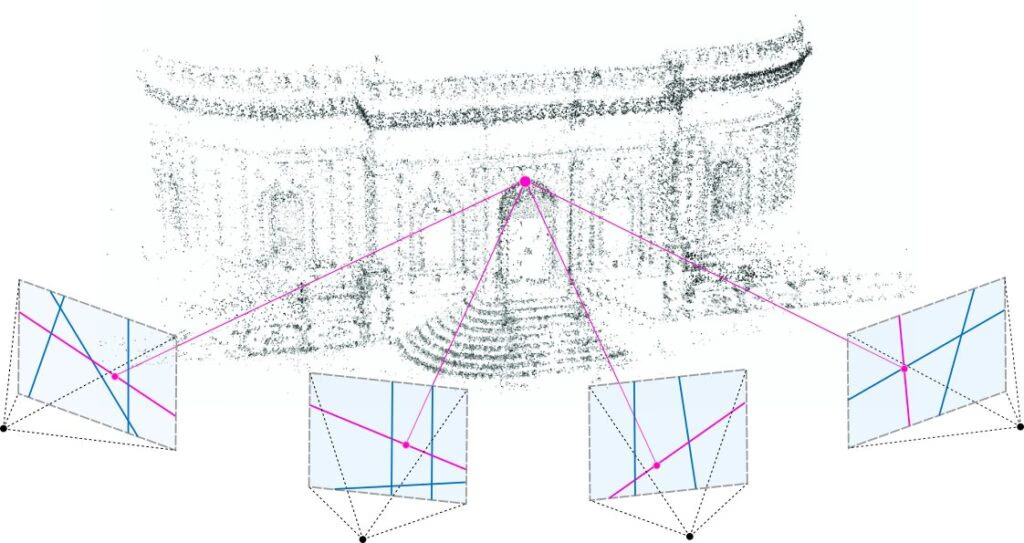
\includegraphics[width=0.9\textwidth]{images/sfm.jpg}
    \caption{Rappresentazione del concetto di Structure From Motion}
    \label{fig:sfm}
    Fonte: \cite{sfm}
\end{figure}
\subsection{COLMAP: implementazione di riferimento per SfM}

COLMAP (COLlaborative Large-scale universal MApping and Positioning) è un framework open-source per Structure from Motion e Multi-View Stereo sviluppato presso l'ETH Zurich. Rappresenta una delle implementazioni più robuste e complete di algoritmi SfM, combinando efficienza computazionale con accuratezza geometrica. COLMAP è diventato lo standard de facto nella comunità di computer vision per la ricostruzione 3D da immagini, supportando una vasta gamma di scenari applicativi.

La pipeline COLMAP implementa un approccio incrementale alla ricostruzione, iniziando con una coppia di immagini ben condizionata e aggiungendo progressivamente nuove viste. Questo metodo garantisce robustezza anche in presenza di scene complesse o dati di input rumorosi. Il sistema integra automaticamente tecniche di bundle adjustment\footnote{Il \emph{bundle adjustment} è una tecnica di ottimizzazione non lineare che raffina simultaneamente tutti i parametri della ricostruzione 3D (posizioni dei punti, pose delle camere e parametri intrinseci) minimizzando l'errore di riproiezione tra i punti ricostruiti e le loro osservazioni nelle immagini.} per l'ottimizzazione simultanea di tutti i parametri, gestione intelligente degli outlier\footnote{Gli \emph{outlier} sono dati errati o rumorosi che non seguono il modello geometrico della scena, come corrispondenze sbagliate tra feature o punti 3D mal triangolati, che devono essere identificati e rimossi per garantire l'accuratezza della ricostruzione.}, e supporto per diversi modelli di camera e condizioni di acquisizione.

Una caratteristica distintiva di COLMAP è la sua capacità di gestire automaticamente molte delle complessità tipiche della ricostruzione SfM, come la selezione delle immagini di inizializzazione, la gestione di scene con componenti disconnesse, e l'identificazione di loop closure\footnote{La \emph{loop closure} è il riconoscimento che la camera è tornata in una posizione già visitata, fondamentale per correggere la deriva accumulata durante la ricostruzione incrementale e migliorare la coerenza globale della scena ricostruita.} in sequenze di immagini. Queste funzionalità rendono COLMAP particolarmente adatto come preprocessing per applicazioni downstream come il 3D Gaussian Splatting.

\subsection{Integrazione COLMAP-3DGS: dal preprocessing al rendering}

La connessione tra COLMAP e 3D Gaussian Splatting è fondamentale e bidirezionale. COLMAP fornisce i dati di input essenziali per tutti gli algoritmi 3DGS, mentre la qualità della ricostruzione COLMAP determina direttamente le prestazioni achievable dai metodi di Gaussian Splatting.

L'output principale di COLMAP utilizzato da 3DGS è la nuvola di punti 3D sparsa, dove ogni punto viene utilizzato per inizializzare una gaussiana 3D. Le coordinate del punto diventano la posizione media della gaussiana, mentre parametri come scala, rotazione e opacità vengono inizializzati utilizzando euristiche. Inoltre, COLMAP fornisce le pose precise delle camere, indispensabili per il processo di rendering differenziabile che costituisce il cuore dell'ottimizzazione 3DGS.

La qualità della ricostruzione COLMAP influenza profondamente le prestazioni finali del sistema 3DGS. Una nuvola di punti densa e accurata fornisce una migliore inizializzazione, riducendo il tempo di convergenza e migliorando la qualità finale. Di contro, errori nella stima delle pose delle camere o nella triangolazione dei punti 3D si propagano attraverso l'intero processo di training, limitando la fedeltà del rendering finale.

È importante notare che COLMAP ricostruisce tipicamente solo i punti più caratteristici e facilmente triangolabili della scena, risultando in una rappresentazione sparsa. Aree uniformi, superfici riflettenti, o regioni con texture insufficiente potrebbero non essere rappresentate nella nuvola di punti iniziale. Questa limitazione è uno dei motivi per cui gli algoritmi 3DGS includono meccanismi di densificazione adattiva durante il training, per colmare le lacune nella rappresentazione iniziale.

\subsection{Requisiti e limitazioni}

Per ottenere risultati di qualità con la pipeline COLMAP-3DGS, è necessario rispettare alcuni requisiti fondamentali nella fase di acquisizione dati. Le immagini devono presentare un overlap sufficiente (tipicamente 60-80\% tra immagini adiacenti) per garantire corrispondenze robuste. La scena deve contenere texture sufficienti per la feature detection, ed è preferibile mantenere condizioni di illuminazione consistenti durante l'acquisizione.

Le limitazioni principali riguardano scene con caratteristiche problematiche per gli algoritmi SfM: superfici uniformi o riflettenti che non generano feature distintive, pattern ripetitivi che possono causare corrispondenze errate, e variazioni di illuminazione drastiche che influenzano la consistenza delle feature. Inoltre, COLMAP, come tutti gli algoritmi SfM, richiede che la scena sia statica durante l'acquisizione.

Nonostante queste limitazioni, la combinazione COLMAP-3DGS rappresenta attualmente la soluzione più matura e affidabile per la generazione di radiance field di alta qualità a partire da immagini multi-vista. La robustezza di COLMAP nella fase di preprocessing, combinata con la capacità dei metodi 3DGS di densificare e raffinare la rappresentazione durante il training, permette di ottenere risultati di qualità eccellente su una vasta gamma di scene reali.

La comprensione di questa pipeline integrata è essenziale per l'utilizzo efficace delle tecniche di 3D Gaussian Splatting, poiché la qualità del preprocessing COLMAP costituisce spesso il fattore limitante per le prestazioni complessive del sistema.

\section{Algoritmi di training utilizzati}

\subsection{Approccio standard (3DGS baseline)}

L'implementazione originale di Kerbl et al. si basa su un approccio di ottimizzazione diretta mediante gradient descent, dove ogni gaussiana 3D viene parametrizzata attraverso posizione, covarianza (scala e rotazione), opacità e coefficienti delle armoniche sferiche per il colore. Il processo di training alterna fasi di ottimizzazione dei parametri gaussiani con operazioni di controllo della densità (densificazione e pruning) per adattare dinamicamente la rappresentazione alla complessità della scena. Questo approccio rappresenta il metodo standard e più consolidato, caratterizzato da semplicità implementativa e robustezza.

\paragraph{Vantaggi chiave}
\begin{itemize}
	\item Risultati stabili e riproducibili
	\item Requisiti hardware accessibili
	\item Buon bilanciamento qualità/prestazioni per scene standard
\end{itemize}

\paragraph{Svantaggi}
\begin{itemize}
	\item Tendenza a generare artefatti "needle-like" in alcune configurazioni
	\item Gestione non ottimale nella distribuzione delle Gaussiane
	\item Difficoltà in scene molto complesse o dense
	\item Controllo limitato sull'allocazione automatica delle risorse
	\item Tendenza a stabilizzarsi in configurazioni subottimali della scena, tipico dei metodi ottimizzati per gradient descent locale
\end{itemize}

\subsection{Monte Carlo Markov Chain: miglioramento qualità tramite campionamento probabilistico}

Il metodo MCMC (Monte Carlo Markov Chain), applicato al training delle Gaussiane 3D, rappresenta un'estensione del metodo originale proposto nel paper fondamentale di 3D Gaussian Splatting. Questo approccio avanzato utilizza una variante chiamata \textbf{Stochastic Gradient Langevin Dynamics (SGLD)} per campionare le configurazioni delle primitive da una distribuzione target, introducendo un rumore stocastico controllato che permette una migliore esplorazione dello spazio delle soluzioni e previene il collasso in minimi locali. Il framework MCMC eredita tutti i parametri in input già elencati in precedenza e ne introduce di aggiuntivi in modo da sfruttare strategie di ottimizzazione più sofisticate.

Inoltre, il metodo include un meccanismo di regolazione della complessità del modello, che consente di controllare dinamicamente il numero di Gaussiane attive durante il training, con l'obiettivo di bilanciare efficacia della rappresentazione e uso efficiente delle risorse computazionali. Questa estensione affronta specificamente alcune limitazioni del metodo originale, come la distribuzione spaziale non ottimale delle Gaussiane e la presenza di Gaussiane "morte" (cioè primitive che cessano di contribuire attivamente al rendering durante il processo di training).

\paragraph{Vantaggi chiave}
\begin{itemize}
	\item Relocazione automatica ed efficace delle Gaussiane non attive
	\item Prevenzione della stagnazione in minimi locali subottimali
	\item Riduzione degli artefatti visivi (needle-like)
	\item Distribuzione spaziale più regolare e adattiva
	\item Migliore esplorazione dello spazio delle soluzioni tramite rumore controllato
\end{itemize}

\paragraph{Svantaggi}
\begin{itemize}
	\item Aumento della complessità implementativa e concettuale
	\item Parametri aggiuntivi da ottimizzare con attenzione
	\item Overhead computazionale dovuto al sampling stocastico
	\item Possibile rallentamento della convergenza se \texttt{noise\_lr} è mal bilanciato
	\item Risultati leggermente meno deterministici a causa dell'introduzione del rumore
\end{itemize}

\subsection{Taming 3DGS: ottimizzazione per risorse computazionali limitate}

Il metodo Taming 3DGS nasce come risposta alle limitazioni computazionali tipiche del Gaussian Splatting su dispositivi non high-end. Il suo contributo principale è l'introduzione di un sistema incrementale e score-guided per la densificazione, in cui ogni nuova Gaussiana viene inserita solo se il suo apporto qualitativo alla scena giustifica il costo computazionale. L'intero processo è regolato da un sistema di punteggio che tiene conto della visibilità, dell'influenza sul gradiente della loss e del contributo alla qualità visiva.

Anche in questo caso, è previsto un sistema di controllo della complessità del modello, che consente di limitare o guidare la crescita del numero di Gaussiane in base a parametri specifici. Questo approccio si traduce in un controllo preciso e prevedibile delle risorse, con implicazioni dirette su tempo, memoria e qualità. L'architettura del metodo evita picchi di memoria durante il training, permettendo la generazione di scene complesse anche su hardware con risorse limitate. Grazie a parametri mirati, è possibile adattare dinamicamente la crescita del modello in funzione della scena e dei vincoli imposti (es. massimo numero di Gaussiane o soglie qualitative minime).
\mbox{}\\
\begin{itemize}
	\item Controllo preciso delle risorse computazionali
	\item Scalabilità su hardware limitato
	\item Processo costruttivo senza picchi di memoria
	\item Densificazione intelligente basata su score
	\item Adattabilità automatica alla complessità della scena
\end{itemize}

\paragraph{Svantaggi}
\begin{itemize}
	\item Possibile perdita di dettagli fini con budget limitati
	\item Complessità aggiuntiva nella configurazione dei parametri
	\item Overhead computazionale per il calcolo degli score
	\item Dipendenza dalla stima accurata dello score di importanza delle gaussiane
	\item Potenziale sottoottimizzazione per rispettare i vincoli di budget
\end{itemize}

\subsection{Parametri di configurazione del training}
I parametri di configurazione permettono di controllare tutti gli aspetti del training nei tre metodi presentati: durata dell'ottimizzazione, gestione delle risorse computazionali e qualità finale del modello. Ogni metodo estende il set di parametri base con opzioni specifiche per le proprie caratteristiche innovative.

I parametri base del 3D Gaussian Splatting (Tabella \ref{tab:3dgs_params}) controllano aspetti fondamentali come numero di iterazioni, risoluzione e densificazione. Il metodo MCMC aggiunge parametri di regolarizzazione (Tabella \ref{tab:mcmc_params}), mentre Taming 3DGS introduce controlli specifici per la gestione delle risorse (Tabella \ref{tab:taming_params}). Le tabelle complete con tutti i parametri e i loro effetti sono riportate nell'Appendice \ref{app:parametri}.


\subsection{Confronto degli approcci}

\begin{table}[h]
	\centering
	\small
	\begin{tabular}{|l|c|c|c|}
		\hline
		\textbf{Criterio} & \textbf{3DGS} & \textbf{MCMC} & \textbf{Taming} \\
		\hline
		Qualità risultato & Buona & Superiore & Adattabile al budget \\
		\hline
		Velocità training & Veloce & Moderata (overhead) & Veloce \\
		\hline
		Uso memoria & Variabile & Controllato & Predicibile \\
		\hline
		Complessità impl. & Bassa & Alta (catena MCMC) & Moderata \\
		\hline
		Requisiti HW & Moderati & Moderati–Alti & Flessibili \\
		\hline
		Stabilità risultati & Alta & Moderata & Alta \\
		\hline
		Controllo risorse & Limitato & Moderato & Eccellente \\
		\hline
	\end{tabular}
	\caption{Confronto tra metodi}
\end{table}

\paragraph{Raccomandazioni d'uso}
\begin{itemize}
	\item \textbf{3DGS Standard}: ideale per applicazioni standard, prototipazione rapida e quando la semplicità implementativa è prioritaria
	\item \textbf{3DGS MCMC}: consigliato per scene complesse dove la qualità è critica e si dispone di risorse computazionali adeguate
	\item \textbf{Taming 3DGS}: ottimale per deployment su hardware limitato, applicazioni real-time e quando il controllo delle risorse è fondamentale
\end{itemize}

\newpage

\section{Metriche di Valutazione}
La valutazione quantitativa della qualità dei modelli 3D generati tramite tecniche di rendering neurale rappresenta una sfida fondamentale nel campo della computer vision. A differenza delle tecniche tradizionali di modellazione 3D, dove la valutazione può concentrarsi su aspetti puramente geometrici, i metodi basati su Gaussian Splatting richiedono metriche che catturino sia la fedeltà visiva che la percezione umana del realismo.

\subsection{Peak Signal-to-Noise Ratio (PSNR)}
Il PSNR rappresenta la metrica più diffusa per la valutazione pixel-wise della qualità di immagini ricostruite. Definito come il rapporto logaritmico tra il valore massimo possibile del segnale e la potenza del rumore di distorsione, il PSNR fornisce una misura oggettiva della fedeltà della ricostruzione:

\begin{equation}
	\text{PSNR} = 10 \cdot \log_{10}\left(\frac{\text{MAX}^2}{\text{MSE}}\right)
\end{equation}

dove MAX rappresenta il valore massimo possibile dei pixel (tipicamente 255 per immagini a 8 bit) e MSE è l'errore quadratico medio tra l'immagine di riferimento e quella ricostruita.

Nel contesto del Gaussian Splatting, il PSNR viene calcolato confrontando le immagini renderizzate dal modello 3D con le immagini ground truth\footnote{Il termine \emph{ground truth} indica i dati di riferimento considerati corretti e accurati, utilizzati come standard per valutare le prestazioni di un algoritmo o modello. Nel contesto del Gaussian Splatting, si riferisce alle immagini originali del dataset di acquisizione.} del dataset di test. Valori più elevati di PSNR indicano una maggiore fedeltà della ricostruzione, con soglie tipiche che considerano acceptable ricostruzioni con PSNR superiore a 20-25 dB per scene complesse.\newline
Nonostante la sua diffusione, il PSNR presenta limitazioni significative nella valutazione della qualità percettiva. La metrica non tiene conto della struttura locale delle immagini né delle caratteristiche del sistema visivo umano, risultando spesso inadeguata per catturare aspetti qualitativi importanti come la nitidezza dei dettagli o la coerenza delle texture.

\subsection{Structural Similarity Index Measure (SSIM)}

Lo SSIM, introdotto da Wang et al., rappresenta un approccio più sofisticato alla valutazione della qualità delle immagini, progettato per correlare meglio con la percezione visiva umana. La metrica opera attraverso la valutazione separata di tre componenti fondamentali del sistema visivo umano, che vengono successivamente combinate in un singolo indice di qualità:

\begin{equation}
	\text{SSIM}(x,y) = [l(x,y)]^{\alpha} \times [c(x,y)]^{\beta} \times [s(x,y)]^{\gamma}
\end{equation}

dove $l(x,y)$, $c(x,y)$ e $s(x,y)$ rappresentano rispettivamente la componente di luminanza, contrasto e struttura, con esponenti $\alpha$, $\beta$, $\gamma$ per controllare l'importanza relativa di ciascuna componente.

I tre componenti sono definiti come:\newline

\textbf{Luminanza}:
\begin{equation}
	l(x,y) = \frac{2\mu_x\mu_y + c_1}{\mu_x^2 + \mu_y^2 + c_1}
\end{equation}

\textbf{Contrasto}:
\begin{equation}
	c(x,y) = \frac{2\sigma_x\sigma_y + c_2}{\sigma_x^2 + \sigma_y^2 + c_2}
\end{equation}

\textbf{Struttura}:
\begin{equation}
	s(x,y) = \frac{\sigma_{xy} + c_3}{\sigma_x\sigma_y + c_3}
\end{equation}

dove $\mu$ rappresenta la media locale, $\sigma$ la deviazione standard locale, $\sigma_{xy}$ la covarianza locale, e $c_1$, $c_2$, $c_3$ sono costanti di stabilizzazione.\newline
Nella pratica, si utilizza comunemente la versione con $\alpha = \beta = \gamma = 1$ e $c_3 = c_2/2$, che produce la formula compatta:

\begin{equation}
	\text{SSIM}(x,y) = \frac{(2\mu_x\mu_y + c_1)(2\sigma_{xy} + c_2)}{(\mu_x^2 + \mu_y^2 + c_1)(\sigma_x^2 + \sigma_y^2 + c_2)}
\end{equation}

I tre componenti valutano aspetti complementari:
\begin{itemize}
	\item \textbf{Luminanza}: Confronto delle intensità medie locali - misura quanto le due immagini sono simili in termini di brillantezza complessiva
	\item \textbf{Contrasto}: Confronto della varianza delle intensità - valuta se le due immagini hanno simili livelli di dettaglio e texture
	\item \textbf{Struttura}: Confronto dei pattern di correlazione spaziale - cattura la similarità nei pattern geometrici e nelle relazioni spaziali tra pixel
\end{itemize}

Lo SSIM produce valori compresi tra -1 e 1, dove 1 indica identità perfetta. Nel rendering neurale, valori SSIM superiori a 0.8-0.9 sono generalmente considerati indicativi di alta qualità visiva.\newline
La separazione in tre componenti consente di diagnosticare specifici aspetti della qualità dell'immagine. Una ricostruzione può avere buona luminanza e contrasto ma struttura degradata, indicando problemi nella preservazione dei dettagli geometrici tipici nelle scene renderizzate con Gaussian Splatting.

\subsection{Learned Perceptual Image Patch Similarity (LPIPS)}

La metrica LPIPS, sviluppata da Zhang et al., rappresenta l'evoluzione più recente nella valutazione percettiva delle immagini, utilizzando reti neurali pre-addestrate per catturare similarità percettive complesse. A differenza delle metriche tradizionali basate su operazioni matematiche dirette sui pixel, LPIPS sfrutta le rappresentazioni apprese da deep network addestrate su task di computer vision.

La metrica opera estraendo feature da diversi layer di reti convoluzionali (tipicamente VGG, AlexNet, o SqueezeNet) e calcolando la distanza pesata tra le rappresentazioni delle immagini da confrontare:

\begin{equation}
	\text{LPIPS} = \sum_l \frac{1}{H_l W_l} \sum_{h,w} ||\mathbf{w}_l \odot (\mathbf{y}^l_{hw} - \mathbf{y}^{l*}_{hw})||_2^2
\end{equation}

dove $l$ indica i layer della rete, $\mathbf{w}_l$ sono pesi appresi, e $\mathbf{y}^l$ rappresenta le feature normalizzate.

\paragraph{Caratteristiche distintive di LPIPS}
\begin{itemize}
	\item \textbf{Sensibilità percettiva}: Cattura distorsioni rilevanti per la percezione umana che sfuggono a metriche tradizionali
	\item \textbf{Robustezza alle trasformazioni}: Meno sensibile a spostamenti pixel-wise che non alterano la percezione
	\item \textbf{Correlazione con giudizi umani}: Elevata correlazione con valutazioni soggettive di qualità
\end{itemize}

Nel contesto del Gaussian Splatting, LPIPS si rivela particolarmente efficace nel distinguere tra ricostruzioni che, pur avendo PSNR/SSIM simili, presentano differenze qualitative significative in termini di realismo e fedeltà percettiva.

\subsection{Applicazione nel Gaussian Splatting}

\subsubsection{Complementarità delle metriche}

L'utilizzo combinato di PSNR, SSIM e LPIPS fornisce una valutazione multi-dimensionale della qualità dei modelli generati:

\begin{itemize}
	\item \textbf{PSNR}: Valutazione della fedeltà pixel-wise e del rumore complessivo
	\item \textbf{SSIM}: Analisi della preservazione delle strutture locali e della coerenza spaziale  
	\item \textbf{LPIPS}: Valutazione della qualità percettiva e del realismo visivo
\end{itemize}

\subsubsection{Sfide specifiche}

La valutazione dei modelli Gaussian Splatting presenta sfide peculiari, ovvero:

\begin{itemize}
	\item \textbf{View-dependence}: A differenza delle immagini statiche, i modelli 3D devono essere valutati da multiple viewpoint, richiedendo l'aggregazione di metriche su diversi punti di vista.
	\item \textbf{Temporal consistency}: Per sequenze video, è necessario valutare anche la coerenza temporale tra frame consecutivi.
	\item \textbf{Scene complexity}: Scene con elementi trasparenti, riflessi o illuminazione complessa possono presentare trade-off diversi tra le metriche.
\end{itemize}

\subsubsection{Benchmark e soglie di Riferimento}

Nel contesto dei dataset standard per la valutazione del Gaussian Splatting (NeRF Synthetic, Mip-NeRF 360, Tanks and Temples), sono emersi range tipici di valori considerati rappresentativi di alta qualità:

\begin{itemize}
	\item \textbf{PSNR}: 25-35 dB per scene indoor, 20-30 dB per scene outdoor
	\item \textbf{SSIM}: 0.85-0.95 per ricostruzioni di alta qualità
	\item \textbf{LPIPS}: 0.05-0.15 (valori più bassi indicano maggiore similarità percettiva)
\end{itemize}

Questi benchmark forniscono riferimenti fondamentali per valutare l'efficacia di nuove varianti algoritmiche e ottimizzazioni implementative nel campo del Gaussian Splatting.

\section{Applicazioni e limitazioni attuali} 
\subsection{Campi di applicazione nella computer vision}
Il 3D Gaussian Splatting trova applicazione in diversi domini:
\begin{itemize}
	\item \textbf{Novel View Synthesis}: è una tecnica che ha l'obiettivo di generare nuove immagini di una scena da punti di vista non osservati direttamente, a partire da un insieme limitato di viste iniziali, sfruttando informazioni spaziali e fotometriche per garantire realismo e coerenza.
	\item \textbf{Digital Content Creation}: Creazione di asset 3D per cinema, gaming e applicazioni VR/AR, sfruttando la velocità di rendering real-time.
	\item \textbf{Simulazione e Digital Twins}: Rappresentazione di ambienti reali per applicazioni industriali, training di sistemi autonomi e visualizzazione architettonica.
	\item 
	\textbf{Medical Imaging}: Ricostruzione di strutture anatomiche da imaging medico, supportando visualizzazione interattiva per diagnosi e pianificazione chirurgica.
\end{itemize}

\subsection{Limiti all’adozione diffusa}
Nonostante i risultati promettenti, l’adozione su larga scala del 3D Gaussian Splatting è ostacolata da numerose \textbf{barriere tecniche e pratiche}.

Dal punto di vista \textit{hardware e computazionale}, la tecnologia richiede GPU moderne per ottenere prestazioni accettabili sia in fase di training che di rendering. Inoltre, i modelli generati possono occupare centinaia di megabyte, specialmente per scene complesse, comportando un \textit{notevole consumo di memoria RAM}, in particolare durante il training di scene su larga scala. La fase di addestramento risulta inoltre sensibile alla qualità dell’input e alla scelta dei parametri di inizializzazione, con un impatto significativo sulla stabilità del processo.

Sul piano \textit{dell’usabilità}, la tecnologia resta ancora confinata prevalentemente all’ambito accademico e specialistico. La documentazione è spesso pensata per un pubblico con background avanzato in \textit{computer graphics} e \textit{machine learning}, rendendo difficile l’approccio per utenti non esperti. L’utilizzo degli strumenti disponibili richiede una \textit{configurazione complessa dell’ambiente} (CUDA, librerie specifiche), una buona comprensione degli \textit{hyperparameter} da ottimizzare manualmente, nonché la gestione di un \textit{workflow articolato} che include preprocessing, training e post-processing. Anche il debugging è tutt’altro che immediato, richiedendo competenze tecniche per interpretare errori e problemi di convergenza.

A queste difficoltà si aggiunge la \textit{frammentazione degli strumenti attualmente disponibili}. Il panorama attuale prevede software e script separati per ogni fase del processo:
\begin{itemize}
    \item \textbf{Framework di training}: spesso legati a implementazioni distinte per ciascuna variante algoritmica;
    \item \textbf{Strumenti di visualizzazione}: viewer non compatibili tra loro o limitati a specifici formati;
    \item \textbf{Utility di preprocessing}: script individuali e poco documentati per la preparazione dei dati;
    \item \textbf{Incoerenza nei formati}: assenza di standard per esportazione e importazione dei modelli.
\end{itemize}

Questa frammentazione ostacola la creazione di workflow fluidi, aumenta la curva di apprendimento per i nuovi utenti e rende più difficile l’adozione industriale della tecnologia. Tali limiti motivano la necessità di piattaforme integrate, come quella proposta in questo lavoro.
\chapter{Architettura del Sistema Proposto}
\label{chap:architettura}

\section{Obiettivi e funzionalità del sistema}
Il sistema proposto è stato progettato per affrontare direttamente le limitazioni per l'adozione diffusa del 3D Gaussian Splatting identificate nel capitolo precedente, trasformando una tecnologia prevalentemente accademica in una soluzione accessibile e user-friendly.

\subsection{Obiettivi di progetto}

\paragraph{Migliore accesso alla tecnologia}
L'obiettivo primario consiste nel rendere il 3D Gaussian Splatting accessibile a utenti senza competenze tecniche specialistiche in computer graphics o machine learning. Il sistema deve eliminare le barriere di ingresso tipiche degli strumenti di ricerca, permettendo a professionisti di settori diversi - dal design alla produzione multimediale - di sfruttare le potenzialità della tecnologia attraverso un'interfaccia intuitiva.

\paragraph{Unificazione di strumenti frammentati}
Il secondo obiettivo riguarda l'integrazione di funzionalità attualmente disperse in implementazioni separate. Il sistema deve fornire una piattaforma unificata che comprenda training, visualizzazione e gestione modelli, eliminando la necessità di utilizzare tool specifici incompatibili tra loro e riducendo significativamente la curva di apprendimento.

\paragraph{Automazione del workflow tecnico}
Il terzo obiettivo è l'automazione dell'intero processo, dalla preparazione dei dati alla visualizzazione finale, riducendo al minimo l'intervento manuale e la possibilità di errori. Questo include la gestione automatica di preprocessing, configurazione parametri e troubleshooting di problemi comuni.

\subsection{Funzionalità del sistema}
Per raggiungere questi obiettivi, il sistema implementa le seguenti funzionalità core:

\paragraph{Interfaccia web guidata}
Il sistema fornisce un'interfaccia web responsive che guida l'utente attraverso un processo step-by-step, dalla selezione del video di input alla visualizzazione del modello 3D finale. L'interfaccia integra:

\begin{itemize}
\item \textbf{Processo guidato}: Workflow sequenziale con istruzioni chiare per ogni fase
\item \textbf{Validazione intelligente}: Controllo automatico della qualità e formato dei file di input
\item \textbf{Feedback}: Indicatore della fase in cui si trovano le elaborazioni
\item \textbf{Documentazione contestuale}: Spiegazioni integrate e suggerimenti per ottimizzare i risultati
\end{itemize}

\paragraph{Training multi-algoritmo integrato}
La piattaforma integra tre diversi approcci di training del Gaussian Splatting in un'unica interfaccia:

\begin{itemize}
\item \textbf{Standard 3DGS}: Implementazione baseline per risultati di alta qualità
\item \textbf{MCMC Gaussian Splatting}: Approccio probabilistico per miglioramento della qualità e riduzione artefatti
\item \textbf{Taming 3DGS}: Ottimizzazione per risorse computazionali limitate
\end{itemize}

L'utente può selezionare l'algoritmo desiderato attraverso un'interfaccia semplificata con parametri preconfigurati per casi d'uso comuni.

\paragraph{Pipeline di processing automatizzata}
Il sistema implementa una pipeline completamente automatizzata che gestisce:

\begin{enumerate}
\item \textbf{Preprocessing video}: Estrazione automatica di frame ottimali dal video di input
\item \textbf{Structure from Motion}: Generazione automatica della point cloud iniziale
\item \textbf{Training asincrono}: Elaborazione in background con notifiche di completamento
\item \textbf{Upload modello}: Upload su repository del modello 3D generato dal training
\item \textbf{Post-processing}: Generazione e salvataggio delle metriche di elaborazione
\end{enumerate}

\begin{figure}[htbp]
	\centering
	\adjustbox{width=0.8\textwidth,center,keepaspectratio}{
		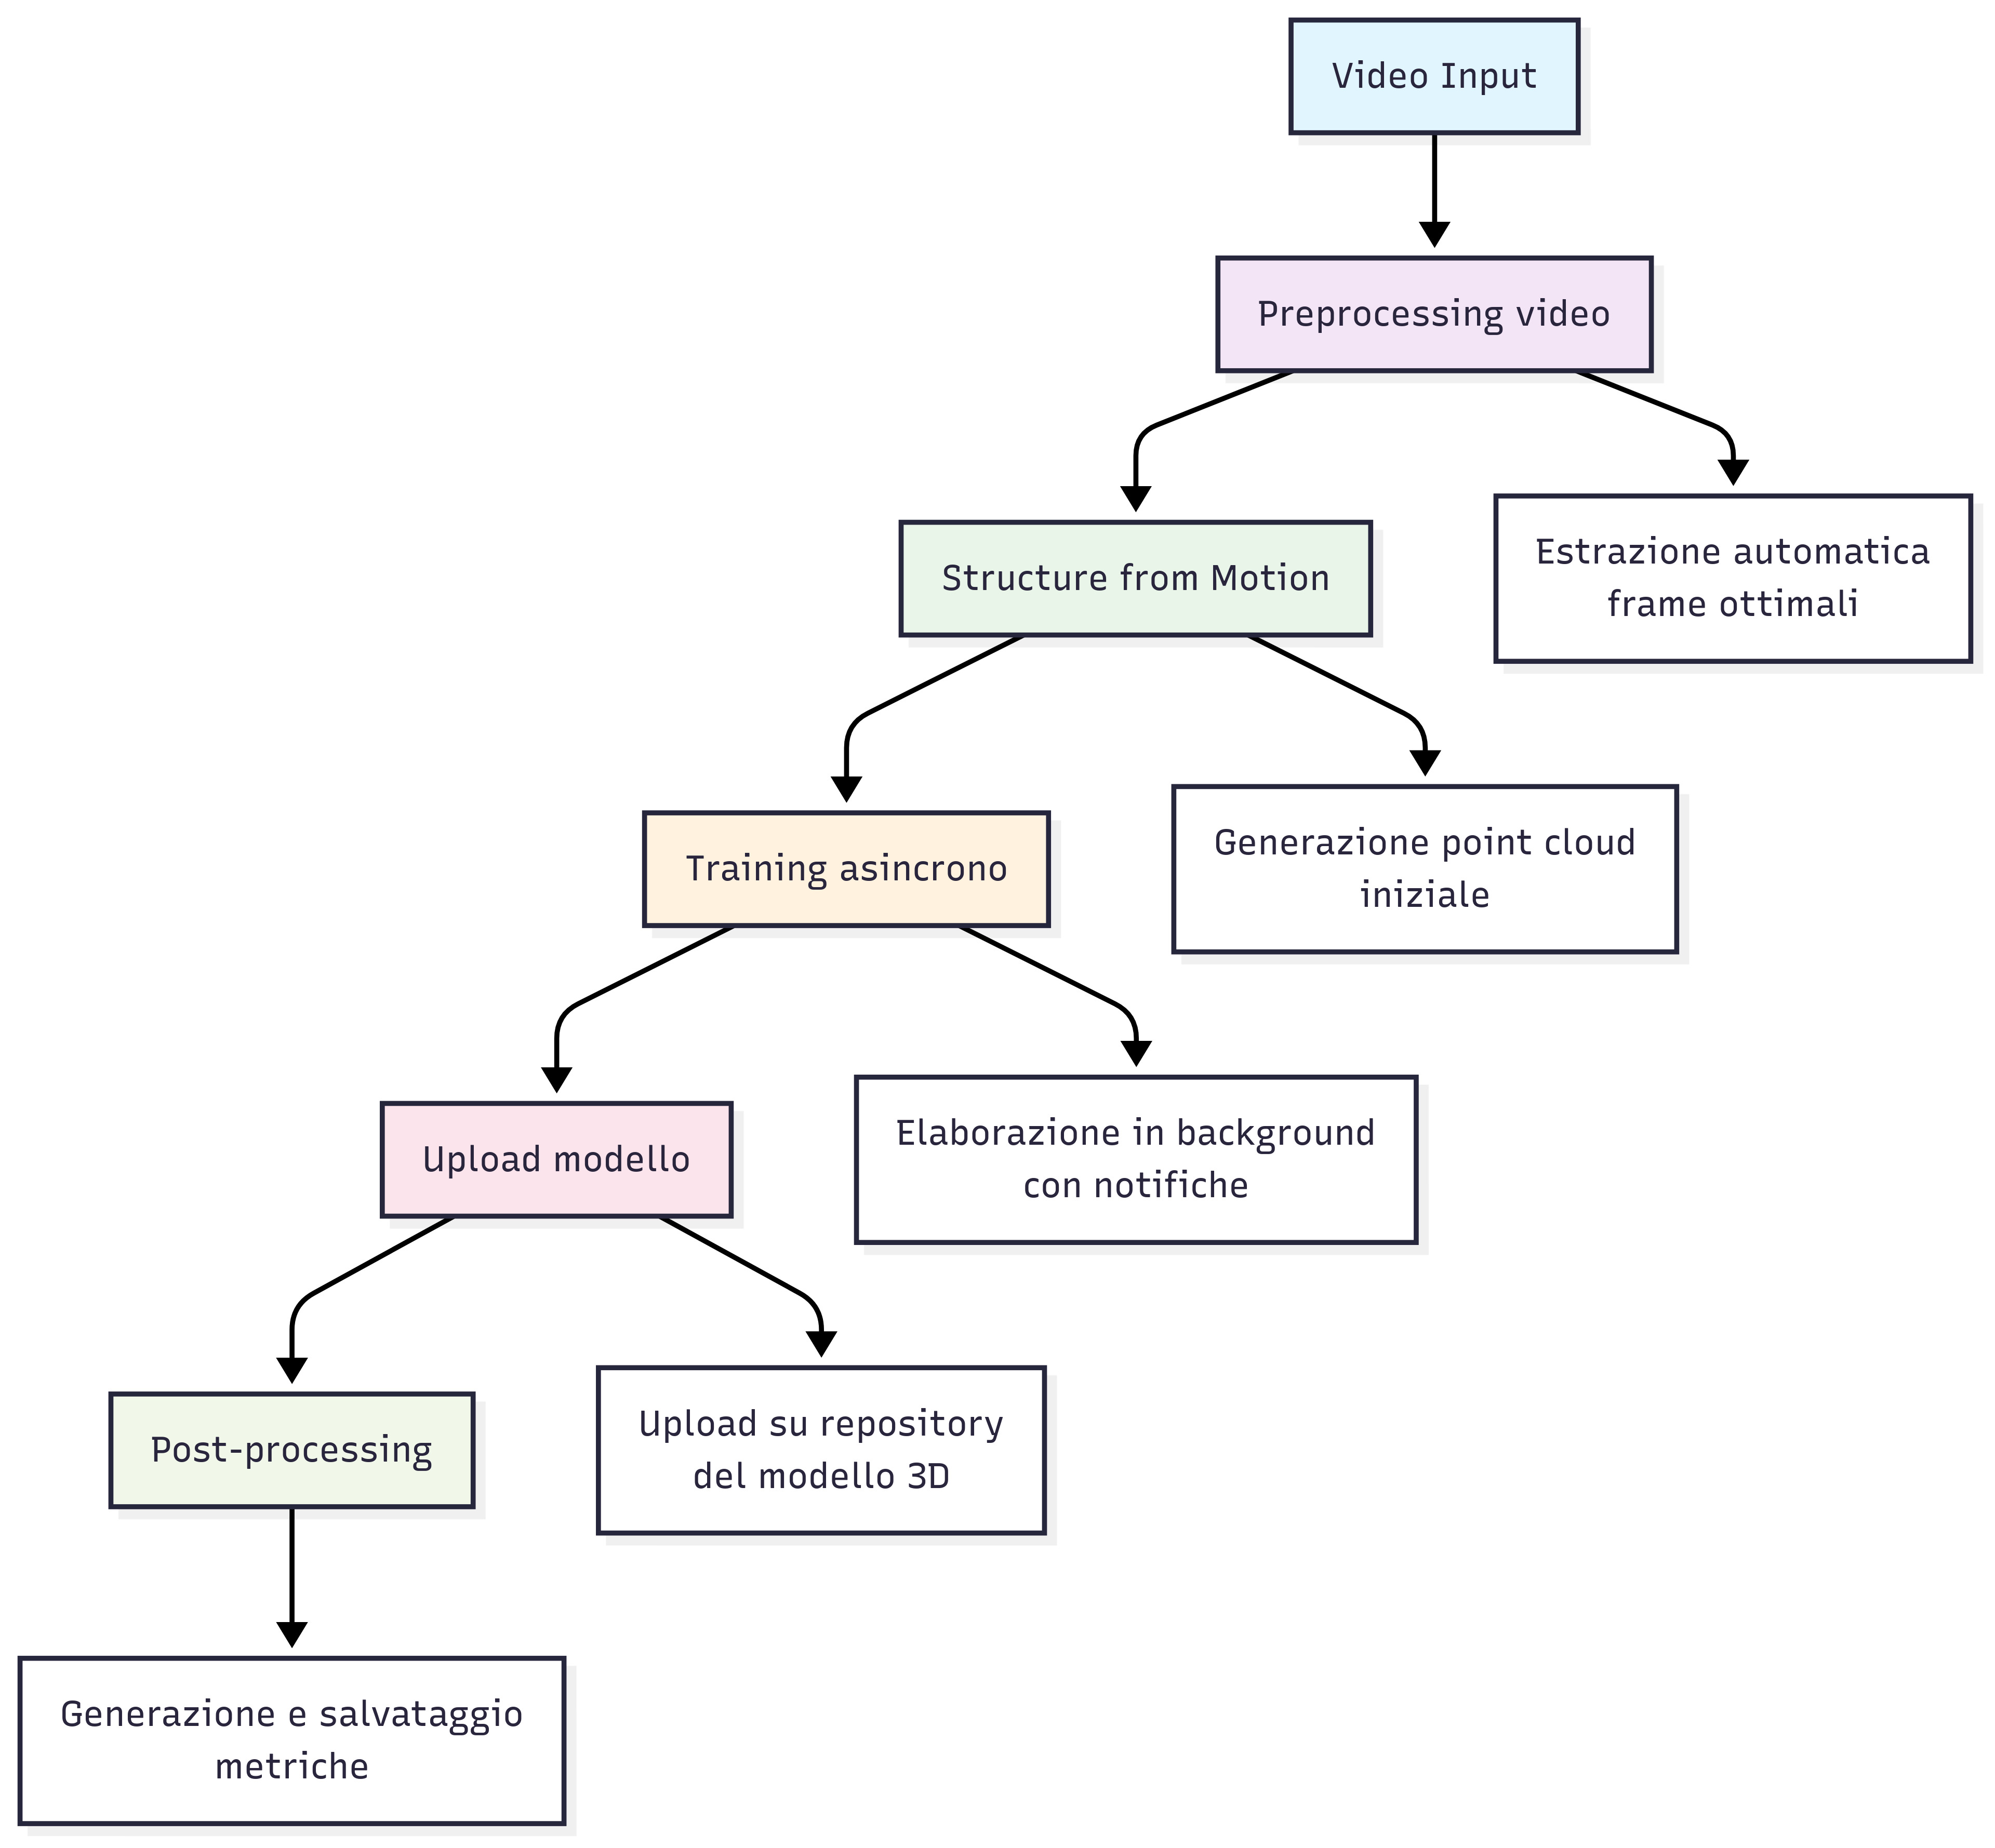
\includegraphics{images/functional_workflow.jpg}
	}
	\caption{Pipeline di processing automatizzata}
	\label{fig:functional_workflow}
\end{figure}

\paragraph{Visualizzazione 3D integrata}
La piattaforma include un viewer 3D web-based che permette:

\begin{itemize}
\item \textbf{Rendering real-time}: Visualizzazione immediata dei modelli generati
\item \textbf{Controlli interattivi}: Navigazione 3D intuitiva con mouse/touch
\item \textbf{Valutazione}: Visualizzazione delle statistiche come FPS e numero di gaussiane generate
\end{itemize}

\paragraph{Gestione trasparente delle risorse}
Il sistema nasconde la complessità tecnica attraverso:

\begin{itemize}
\item \textbf{Containerizzazione}: Ambiente di esecuzione isolato e riproducibile
\item \textbf{Gestione automatica GPU}: Allocazione ottimale delle risorse computazionali
\item \textbf{Scaling adattivo}: Gestione automatica del carico di lavoro
\item \textbf{Monitoring integrato}: Raccolta automatica di metriche di performance e qualità
\end{itemize}

\subsection{Benefici attesi}

L'implementazione di queste funzionalità mira a produrre i seguenti benefici:
\begin{itemize}
    \item \textbf{Riduzione time-to-market}: Dalla creazione del contenuto alla visualizzazione 3D in minuti invece che ore o giorni richiesti da workflow tradizionali.
    \item \textbf{Accessibilità ampliata}: Estensione dell'utilizzo del 3D Gaussian Splatting a settori non tecnici come marketing, e-commerce, architettura e produzione di contenuti.
    \item \textbf{Standardizzazione del processo}: Etablishment di best practices e workflow standardizzati per la creazione di contenuti 3D da video.
    \item \textbf{Riduzione costi}: Eliminazione della necessità di competenze specialistiche dedicate e riduzione dei tempi di training del personale.
\end{itemize}

\section{Organizzazione a Layer}

Il sistema proposto implementa un'architettura distribuita a microservizi progettata per gestire l'intero workflow del 3D Gaussian Splatting, dall'upload del contenuto video alla visualizzazione dei modelli 3D generati. La Figura \ref{fig:system_architecture} presenta una vista complessiva dell'architettura, evidenziando i componenti principali e i loro pattern di interazione.
L'architettura è strutturata in layer distinti, ciascuno con responsabilità specifiche e interfacce ben definite, seguendo i principi di separazione delle responsabilità e scalabilità indipendente. Questa organizzazione logica non implica una separazione fisica rigida, ma piuttosto una strutturazione delle responsabilità che può essere implementata all'interno di uno o più servizi containerizzati.

\begin{figure}[htbp]
	\centering
	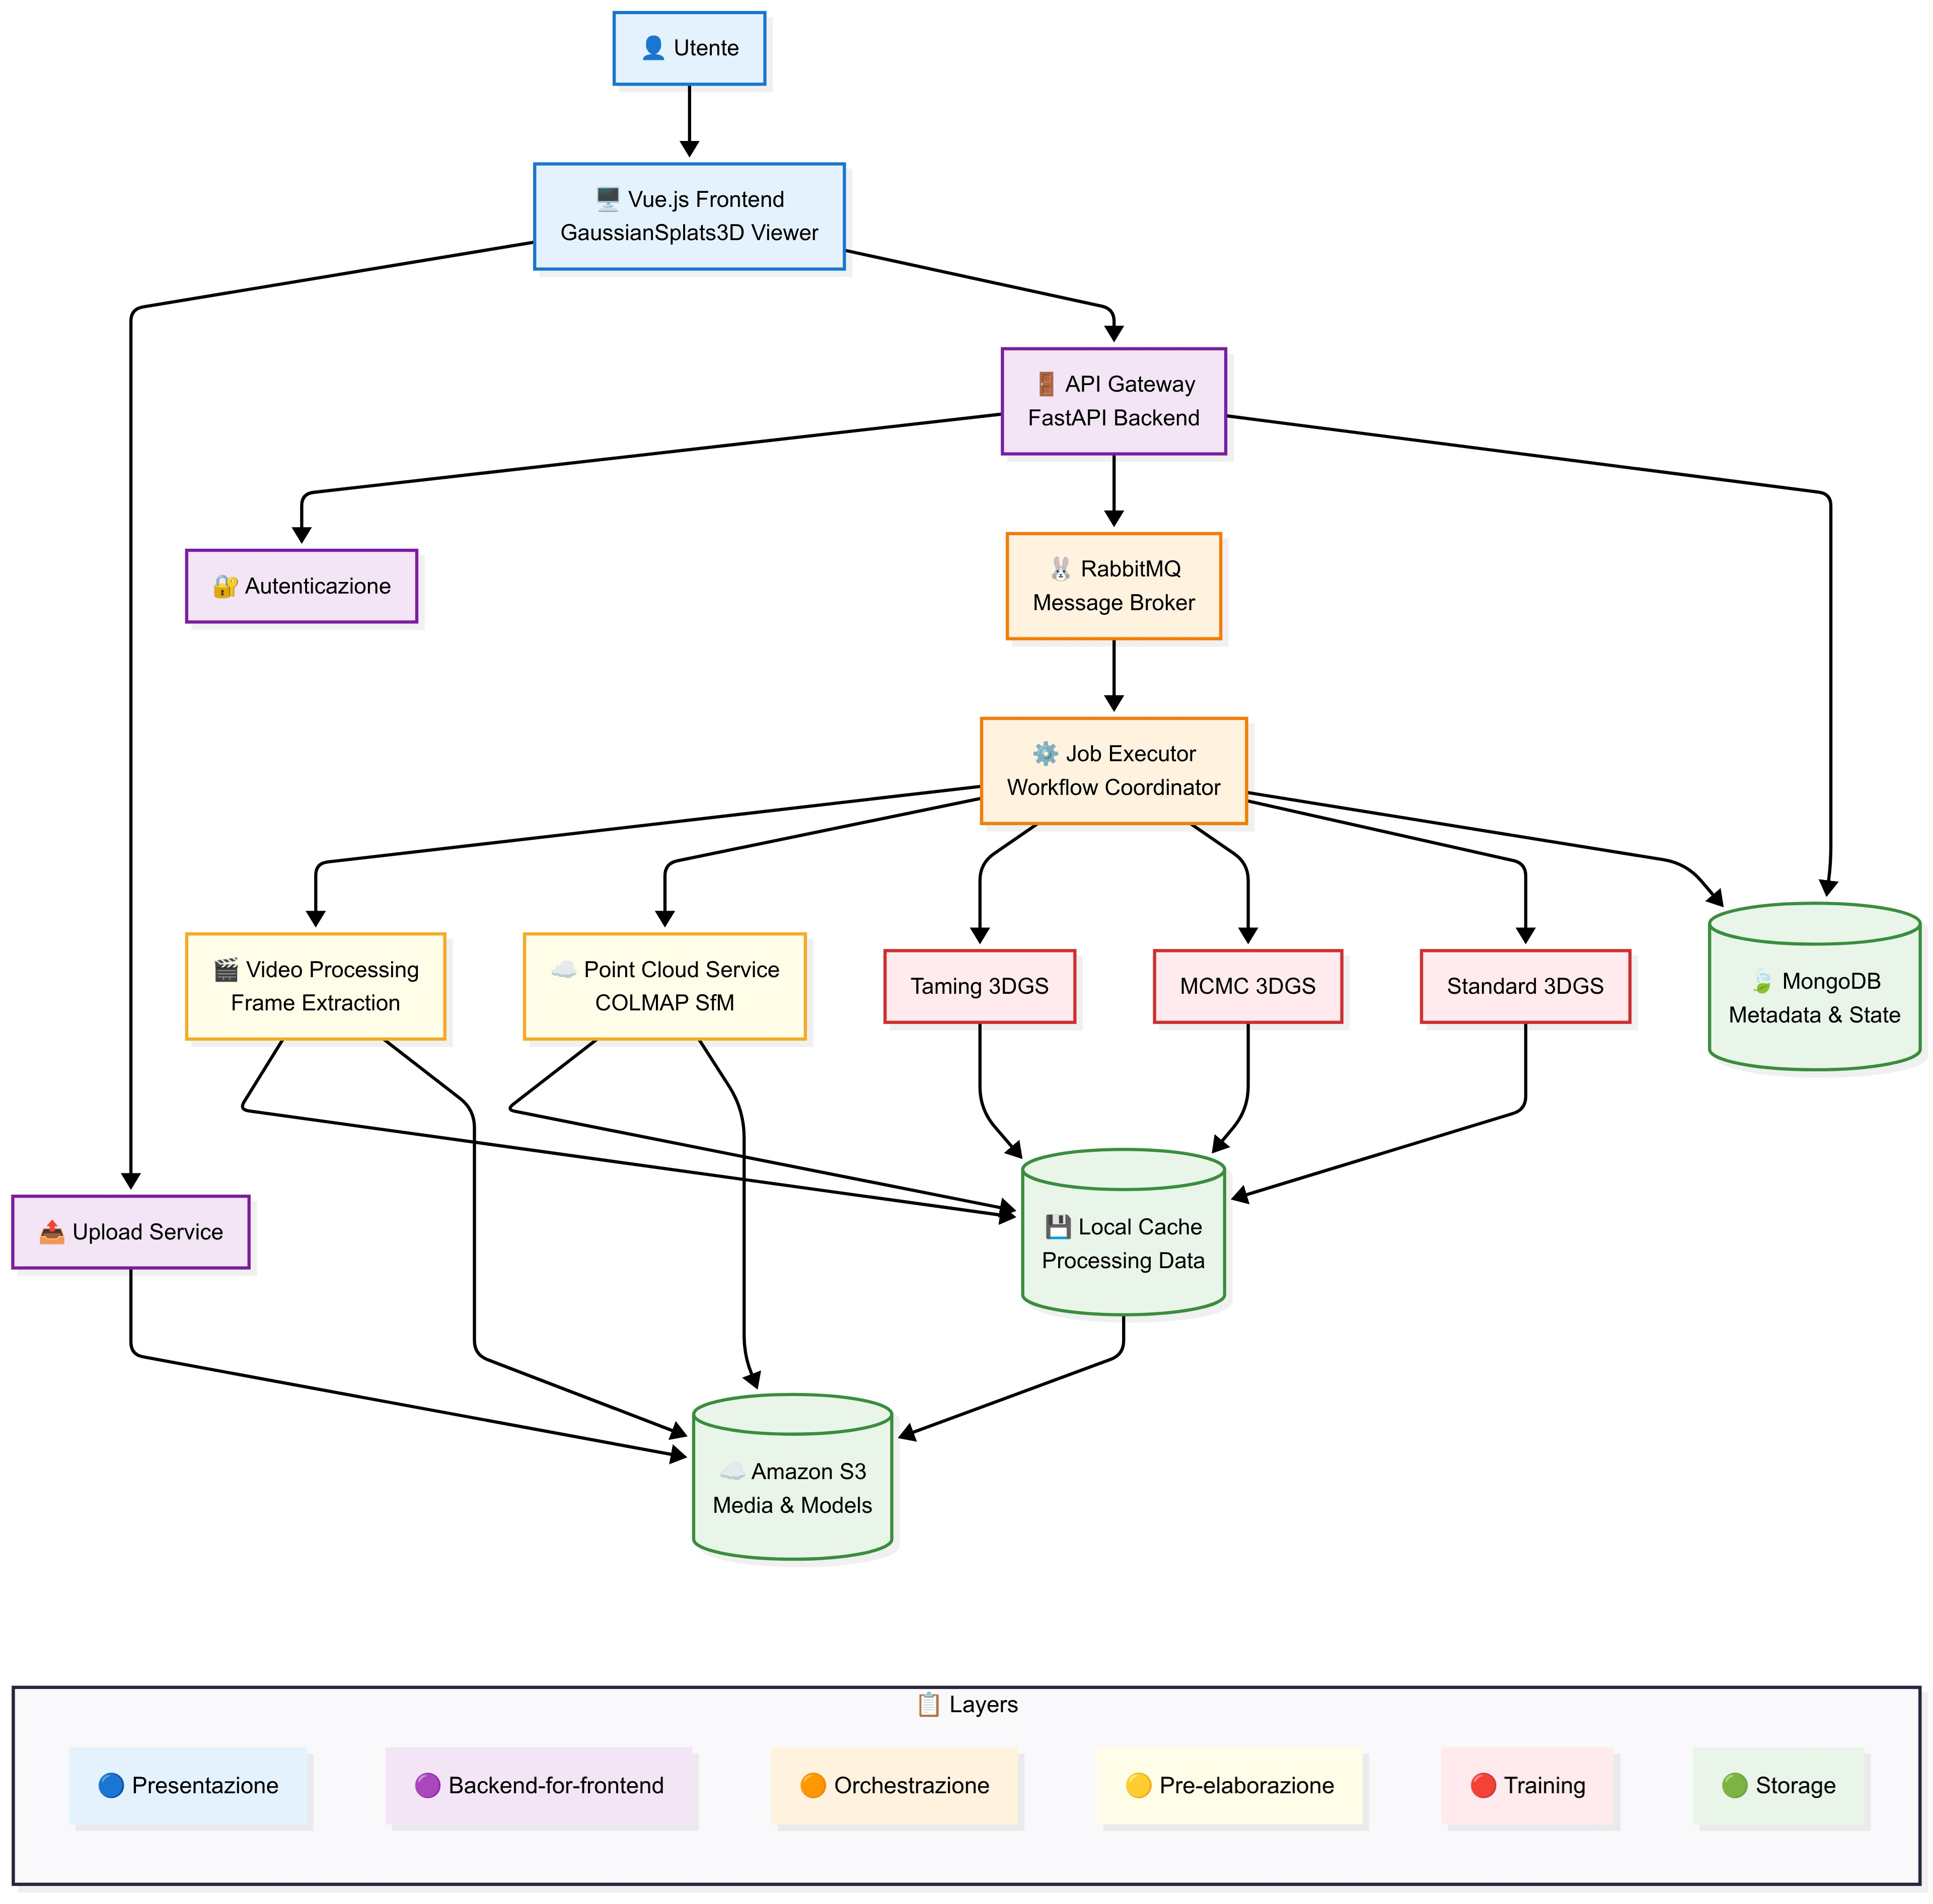
\includegraphics[width=\textwidth]{images/diagramma_architettura.jpg}
	\caption{Architettura complessiva del sistema distribuito}
	\label{fig:system_architecture}
\end{figure}


\subsection{Layer di Storage}

Il \textbf{layer di storage} implementa una strategia ibrida che combina MongoDB per metadati e stato delle elaborazioni, Amazon S3 per contenuti multimediali e modelli 3D che si appoggia a sua volta ad una cache locale per dati di processing temporanei.

\subsection{Layer di Orchestrazione}

Il \textbf{layer di orchestrazione} rappresenta il cuore coordinativo del sistema, implementato attraverso RabbitMQ come message broker e il Job Executor come coordinatore del workflow. Questo layer gestisce la comunicazione asincrona tra i componenti e implementa un pattern Producer-Consumer ibrido che garantisce l'esecuzione sequenziale delle fasi di elaborazione. La scelta di RabbitMQ assicura persistenza dei messaggi, gestione delle code specializzate e resilienza in caso di fallimenti temporanei.

\subsection{Layer di Pre-elaborazione}
Il \textbf{layer di preprocessing} comprende i servizi specializzati responsabili dell'elaborazione preliminare dei dati: Video Processing per l'estrazione dei frame dal video di input e Point Cloud Service per la ricostruzione geometrica tramite COLMAP SfM.

\subsection{Layer di Training}
Il \textbf{layer di training} include i Training Services che eseguono gli algoritmi di Gaussian Splatting nelle diverse implementazioni (Taming 3DGS, MCMC 3DGS e Standard 3DGS), utilizzando le risorse computazionali GPU per l'addestramento dei modelli.

\subsection{Layer Backend-for-Frontend}
Il \textbf{layer Backend-for-Frontend} funge da punto di ingresso unificato per tutte le richieste del sistema, implementando pattern di routing, autenticazione e gestione delle richieste. Questo layer è univocamente rappresentato dall'applicazione (e container) API Gateway, è sviluppata in FastAPI ed espone endpoint REST standardizzati permettendo l'accesso ai servizi sottostanti.

\subsection{Layer di Presentazione}
Il \textbf{layer di presentazione} costituisce l'interfaccia utente del sistema e comprende l'applicazione web sviluppata in Vue.js integrata con il viewer GaussianSplats3D. Questo layer gestisce l'interazione utente, la visualizzazione dei modelli generati e la gestione degli stati dell'interfaccia. La scelta di Vue.js consente un'architettura component-based leggera che facilita la manutenibilità e l'estensibilità dell'interfaccia.

\section{Principi e pattern architetturali}

\subsection{Principi di design}
L'architettura del sistema è stata progettata rispondendo alle sfide specifiche del 3D Gaussian Splatting come tecnologia emergente. A differenza delle applicazioni web tradizionali, il Gaussian Splatting presenta caratteristiche uniche che richiedono decisioni architetturali mirate: elaborazioni GPU-intensive con tempi variabili da minuti a ore, algoritmi in rapida evoluzione, gestione di contenuti multimediali di grandi dimensioni e necessità di isolamento per operazioni hardware-critical.

I principi di design adottati mirano a trasformare una tecnologia di ricerca complessa in una piattaforma accessibile e robusta. L'approccio privilegia la separazione delle preoccupazioni per isolare la complessità computazionale dalle interfacce utente, la scalabilità selettiva per ottimizzare l'uso di risorse costose, e la modularità per facilitare l'integrazione di nuovi algoritmi e l'evoluzione del sistema nel tempo.

Questi principi si concretizzano in scelte implementative specifiche che bilancino semplicità d'uso, efficienza operativa e flessibilità tecnica.

\subsubsection{Separazione delle responsabilità per processing intensivo}
Sebbene un'architettura monolitica possa gestire processing asincrono 
attraverso threading, l'approccio a microservizi offre vantaggi specifici 
per il Gaussian Splatting: isolamento degli errori hardware-intensive, 
scalabilità selettiva delle risorse GPU, e deployment indipendente di 
algoritmi in evoluzione.
L'approccio a microservizi permette di separare logicamente:

\begin{itemize}
    \item \textbf{Servizi di interfaccia}: Frontend e API che rimangono sempre responsivi
    \item \textbf{Servizi di processing}: Dedicati esclusivamente al training intensivo
    \item \textbf{Servizi di supporto}: Gestione dati, code messaggi e storage
\end{itemize}


Queste funzionalità si traducono in un'architettura tecnica specifica che verrà dettagliata nelle sezioni successive, dimostrando come gli obiettivi di alto livello si concretizzino in scelte implementative precise.

\begin{figure}[htbp]
	\centering
	\adjustbox{width=0.9\textwidth,center,keepaspectratio}{
		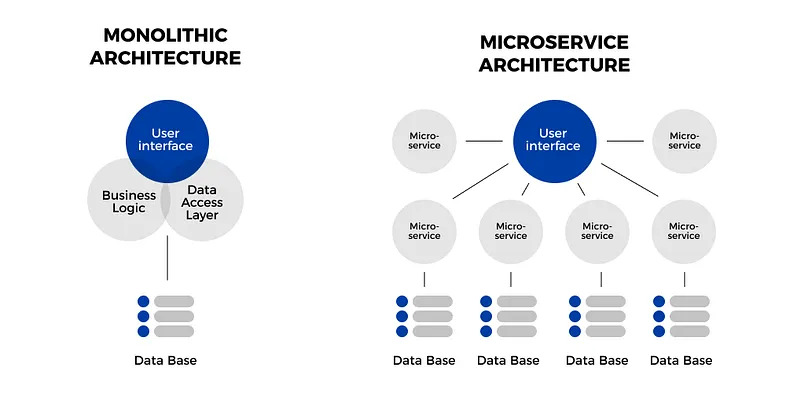
\includegraphics{images/monolith_vs_microservices.jpg}
	}
	\caption{Architettura monolita vs architettura a microservizi}
	\label{fig:monolith_vs_microservices}
\end{figure}

\subsubsection{Scalabilità orizzontale specializzata}
La natura del training di Gaussian Splatting, che richiede hardware dedicato (GPU), rende particolarmente vantaggiosa la possibilità di scalare orizzontalmente solo i componenti computazionalmente intensivi. I servizi di training, essendo containerizzati e stateless, possono essere deployati su multiple macchine dotate di GPU specializzate, mentre frontend e API rimangono centralizzati su hardware meno specializzato.
Questa separazione consente di:

\begin{itemize}
    \item \textbf{Ottimizzare i costi}: hardware GPU costoso utilizzato solo per training e il preprocessing
    \item \textbf{Gestire il carico}: aAggiungere capacità computazionale senza modificare altri servizi
    \item \textbf{Isolamento degli errori}: crash o indisponibilità del training non compromette l'interfaccia utente
\end{itemize}

\subsubsection{Deployment e manutenzione indipendente}
L'architettura modulare facilita lo sviluppo e la manutenzione del sistema, permettendo di aggiornare, testare e deployare ogni componente indipendentemente. Questo è particolarmente vantaggioso per un progetto che integra algoritmi di training in evoluzione (Standard, MCMC, Taming), dove ogni implementazione può essere aggiornata senza impattare gli altri moduli.

\begin{figure}[htbp]
	\centering
	\adjustbox{width=0.9\textwidth,center,keepaspectratio}{
		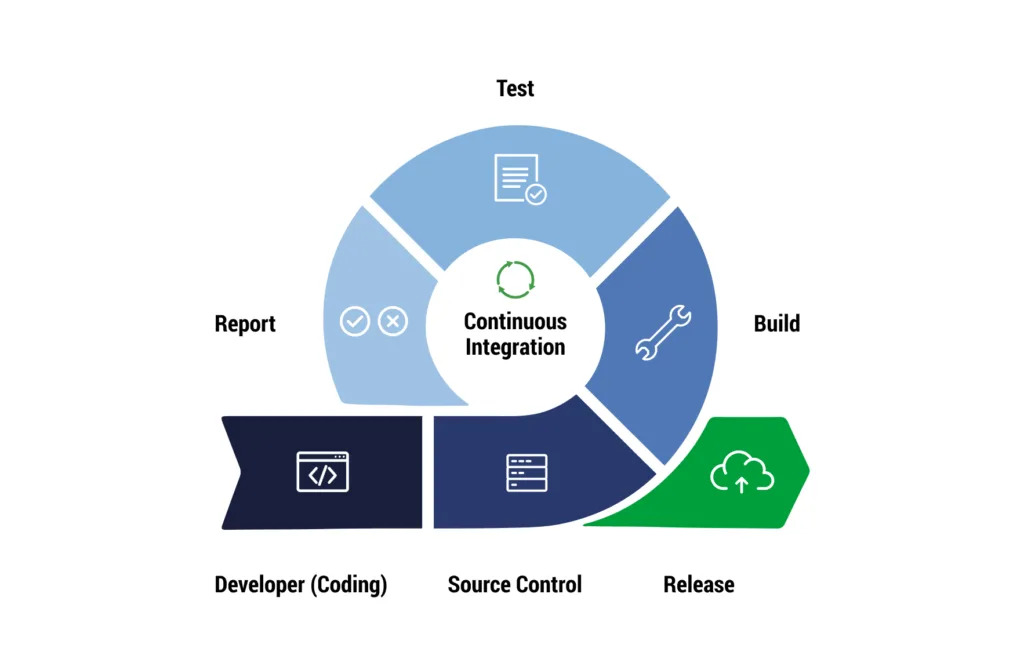
\includegraphics{images/continuous_integration.jpg}
	}
	\caption{Schema della continuous integration}
	\label{fig:continuous_integration}
\end{figure}

\subsection{Pattern architetturali implementati}

Per realizzare i principi di design descritti, il sistema adotta pattern architetturali consolidati, adattati alle specifiche esigenze del 3D Gaussian Splatting. Questi pattern forniscono soluzioni concrete per gestire la complessità del workflow, garantire la resilienza del sistema e ottimizzare l'uso delle risorse computazionali.

I pattern selezionati operano sinergicamente per creare un'architettura che supporta elaborazioni asincrone lunghe, gestione robusta degli errori e scalabilità delle operazioni intensive.

\subsubsection{Architettura Event-driven}
Il sistema implementa un'architettura guidata dagli eventi attraverso una coda di messaggi che coordina l'esecuzione delle diverse fasi di processing. Ogni completamento di fase genera un evento che triggera la fase successiva, creando un workflow asincrono e resiliente.\newline\newline
\textbf{Vantaggi per il Gaussian Splatting}:
\begin{itemize}
	\item \textbf{Gestione della coda}: Serializzazione automatica dei job per gestire la limitazione di GPU singola
	\item \textbf{Retry automatico}: Eventi possono essere riaccodati in caso di fallimento
	\item \textbf{Monitoring}: Stato del workflow tracciabile attraverso gli eventi
\end{itemize}

\begin{figure}[htbp]
	\centering
	\adjustbox{width=0.9\textwidth,center,keepaspectratio}{
		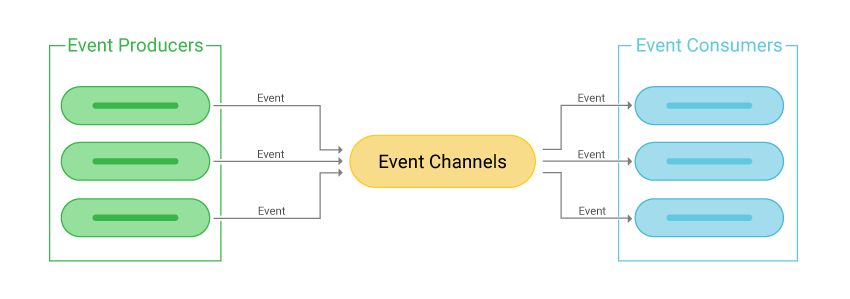
\includegraphics{images/event_driven_architecture.jpg}
	}
	\caption{Architettura Event-driven}
	\label{fig:event_driven_architecture}
\end{figure}

\subsubsection{Pipeline Pattern}
Il processing del Gaussian Splatting segue naturalmente un pattern pipeline con handoff espliciti tra fasi:

\begin{itemize}
	\item \textbf{Estrazione frame} → Output: frame video + metadati
	\item \textbf{Structure from Motion} → Output: point cloud + pose camere
	\item \textbf{Training} → Output: modello 3D ottimizzato
\end{itemize}

Ogni fase produce output standardizzati che vengono consumati dalla fase successiva, permettendo parallelizzazione e reprocessing selettivo.

\subsubsection{Caching e Storage Pattern}

Il sistema adotta una strategia di gestione dati multi-livello che combina diversi pattern architetturali per ottimizzare prestazioni, resilienza e ciclo di vita dei contenuti multimediali. L'approccio integra tre pattern complementari specificamente adattati alle caratteristiche del 3D Gaussian Splatting.

\paragraph{Cache-Aside Pattern per performance}
Il sistema implementa una strategia di caching a due livelli per ridurre latenza e costi di accesso ai dati:

\begin{algorithm}[h]
	\caption{Cache-Aside Pattern per gestione risorse}
	\SetAlgoLined
	\KwIn{resource\_identifier}
	\KwOut{resource\_data}
	
	\eIf{resource exists in local\_cache}{
		\Return{load\_from\_local\_cache(resource\_identifier)}\;
	}{
		resource\_data $\leftarrow$ fetch\_from\_remote\_storage(resource\_identifier)\;
		save\_to\_local\_cache(resource\_identifier, resource\_data)\;
		\Return{resource\_data}\;
	}
\end{algorithm}

Questo approccio è particolarmente efficace per file di grandi dimensioni tipici del Gaussian Splatting, riducendo significativamente i costi e i tempi di accesso a S3 durante le operazioni intensive.

\paragraph{Staging Pattern per persistenza intermedia}
Amazon S3 funge da storage intermedio tra le fasi del workflow, implementando un pattern staging che garantisce:

\begin{itemize}
	\item \textbf{Persistenza}: Risultati intermedi sopravvivono a restart dei servizi
	\item \textbf{Reprocessing selettivo}: Possibilità di ripartire da fasi specifiche già completate
	\item \textbf{Auditability}: Tracciabilità completa dei dati prodotti durante l'elaborazione
\end{itemize}

\paragraph{Hybrid Storage per ciclo di vita dati}
La strategia combina diversi livelli di storage ottimizzati per i pattern di accesso specifici del Gaussian Splatting:

\begin{itemize}
	\item \textbf{Storage locale}: Cache temporanea per elaborazioni attive con accesso veloce, riduzione latenza I/O e cleanup automatico
	\item \textbf{Amazon S3 Standard}: Repository persistente per video originali e modelli finali con durabilità, scalabilità e versioning
	\item \textbf{Processing cache}: Dati intermedi (frame, point clouds) mantenuti localmente per supportare reprocessing parziale
\end{itemize}

L'architettura mantiene tutti i dati persistenti per massimizzare la flessibilità operativa, privilegiando la funzionalità di reprocessing e la semplicità gestionale. Questo approccio conservativo garantisce la stabilità del workflow, elemento centrale per l'esperienza utente del sistema.
\newpage
\section{Containerizzazione con Docker e Docker Compose}
\subsection{Isolamento delle dipendenze specializzate}
Ogni algoritmo di training del Gaussian Splatting presenta dipendenze specifiche e spesso conflittuali:

\begin{itemize}
    \item \textbf{Versioni CUDA}: Diverse implementazioni richiedono versioni specifiche di CUDA (driver NVIDIA)
    \item \textbf{Librerie Python}: Conflitti tra versioni di PyTorch, NumPy e librerie di computer vision
    \item \textbf{Configurazioni hardware}: Ottimizzazioni specifiche per GPU diverse
\end{itemize}

\subsection{Orchestrazione con Docker Compose}
Docker Compose facilita la gestione dell'intero stack applicativo, definendo in modo dichiarativo:

\begin{itemize}
    \item \textbf{Networking}: Comunicazione sicura tra container
    \item \textbf{Volume mounting}: Condivisione dati tra servizi
    \item \textbf{Environment variables}: Configurazione centralizzata
    \item \textbf{Service dependencies}: Ordine di avvio dei servizi
\end{itemize}

Sebbene il deployment attuale avvenga su singola macchina per ragioni di sviluppo, l'architettura containerizzata prepara il sistema per un futuro deployment distribuito su cluster.

\subsection{Gestione risorse GPU}
La containerizzazione permette di gestire in modo granulare l'accesso alle risorse GPU, garantendo che il container di training abbia accesso esclusivo alle GPU disponibili, evitando conflitti di risorse e ottimizzando le performance.

\begin{figure}[htbp]
	\centering
	\adjustbox{width=0.9\textwidth,center,keepaspectratio}{
		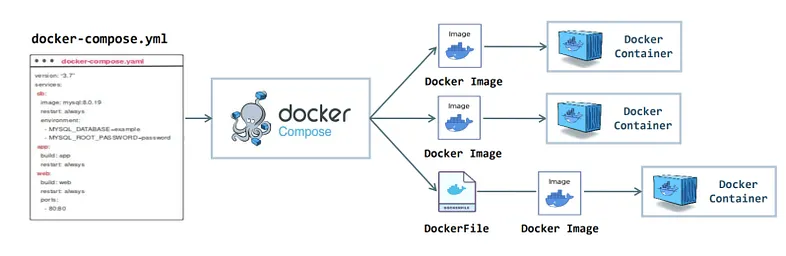
\includegraphics{images/docker_compose.jpg}
	}
	\caption{Architettura con Docker Compose}
	\label{fig:docker_compose}
\end{figure}

\newpage

\section{Gestione asincrona e code messaggi}
Il sistema adotta un'architettura di messaggistica progettata per l'efficienza e la robustezza. La strategia centrale consiste nel separare completamente i dati dai messaggi di controllo: le code contengono esclusivamente identificativi dei modelli, mentre MongoDB centralizza tutti i parametri e lo stato di esecuzione.

\subsection{Code leggere per workflow complessi}
Ogni fase del pipeline (estrazione, SfM, training) utilizza una coda dedicata che trasporta solo gli ID dei modelli da processare. Questa scelta elimina la duplicazione di dati nelle code e mantiene i messaggi estremamente compatti, migliorando le prestazioni del sistema di messaggistica anche con carichi intensivi.

\subsection{Stato sempre sincronizzato}
All'avvio di ogni fase, il servizio responsabile interroga MongoDB per recuperare configurazione, stato precedente e metadati aggiornati. Questo pattern garantisce che ogni elaborazione operi sempre sui dati più recenti, eliminando inconsistenze dovute a messaggi obsoleti o duplicati.

\subsection{Resilienza e reprocessing selettivo}
I fallimenti vengono gestiti con arresti controllati che preservano lo stato raggiunto, consentendo analisi dettagliate e retry mirati. Il sistema supporta riprocessing selettivo: un modello può essere rigenerato partendo da qualsiasi fase già completata, evitando elaborazioni ridondanti e ottimizzando l'utilizzo delle risorse GPU.

Questo design bilancia efficienza computazionale e flessibilità operativa, requisiti essenziali per un sistema di produzione dedicato al 3D Gaussian Splatting.

\section{Flusso di elaborazione end-to-end}
Il flusso di elaborazione del sistema segue un approccio sequenziale orchestrato attraverso code di messaggi specializzate. Ogni fase del workflow è gestita da job specifici che, una volta completati, innescano automaticamente la fase successiva della pipeline.
\subsection{Fase di Upload e Inizializzazione}
Il processo inizia con l'upload del video da parte dell'utente attraverso il frontend. Il sistema implementa un meccanismo di upload sicuro basato su presigned URL: il frontend richiede al backend un URL temporaneo per il caricamento diretto sull'object storage, evitando il transito del contenuto multimediale attraverso il backend API. Completato l'upload, il frontend effettua una richiesta POST di creazione del modello, specificando i parametri di training (algoritmo, livello di qualità, nome progetto).
\subsection{Pipeline di Elaborazione}
Il backend persiste i metadati del nuovo modello nel database e inserisce il primo job della catena nella coda di messaggi. Il flusso di elaborazione è strutturato in cinque fasi sequenziali:
\begin{enumerate}
\item \textbf{Frame Extraction}: estrazione dei frame dal video caricato
\item \textbf{Cloud Point Reconstruction}: generazione della nuvola di punti iniziale
\item \textbf{Training}: esecuzione dell'algoritmo di Gaussian Splatting selezionato
\item \textbf{Upload}: caricamento del modello 3D generato sull'object storage
\item \textbf{Metrics Generation}: calcolo delle metriche di qualità del modello
\end{enumerate}
\paragraph{Coordinamento tra Job}
Il sistema adotta un'architettura a code specializzate, dove ogni tipologia di job dispone di una coda dedicata. Al completamento di ciascun job, il job executor inserisce automaticamente il task successivo nella coda appropriata, garantendo la continuità del flusso di elaborazione. Questa architettura permette una gestione granulare delle risorse e una scalabilità indipendente per ogni fase del workflow.
\paragraph{Gestione dei Fallimenti}
In caso di fallimento di un job, il flusso di elaborazione si interrompe e il modello viene marcato con stato di errore. Il sistema non implementa meccanismi automatici di retry, ma permette all'utente di riavviare manualmente l'elaborazione dal frontend, sfruttando la funzionalità di clonazione del modello per ripartire da eventuali step già completati con successo.


\begin{figure}[htbp]
\centering
\vspace*{-1cm} % Riduci spazio sopra la figura
\adjustbox{width=0.5\textwidth,center,keepaspectratio}{
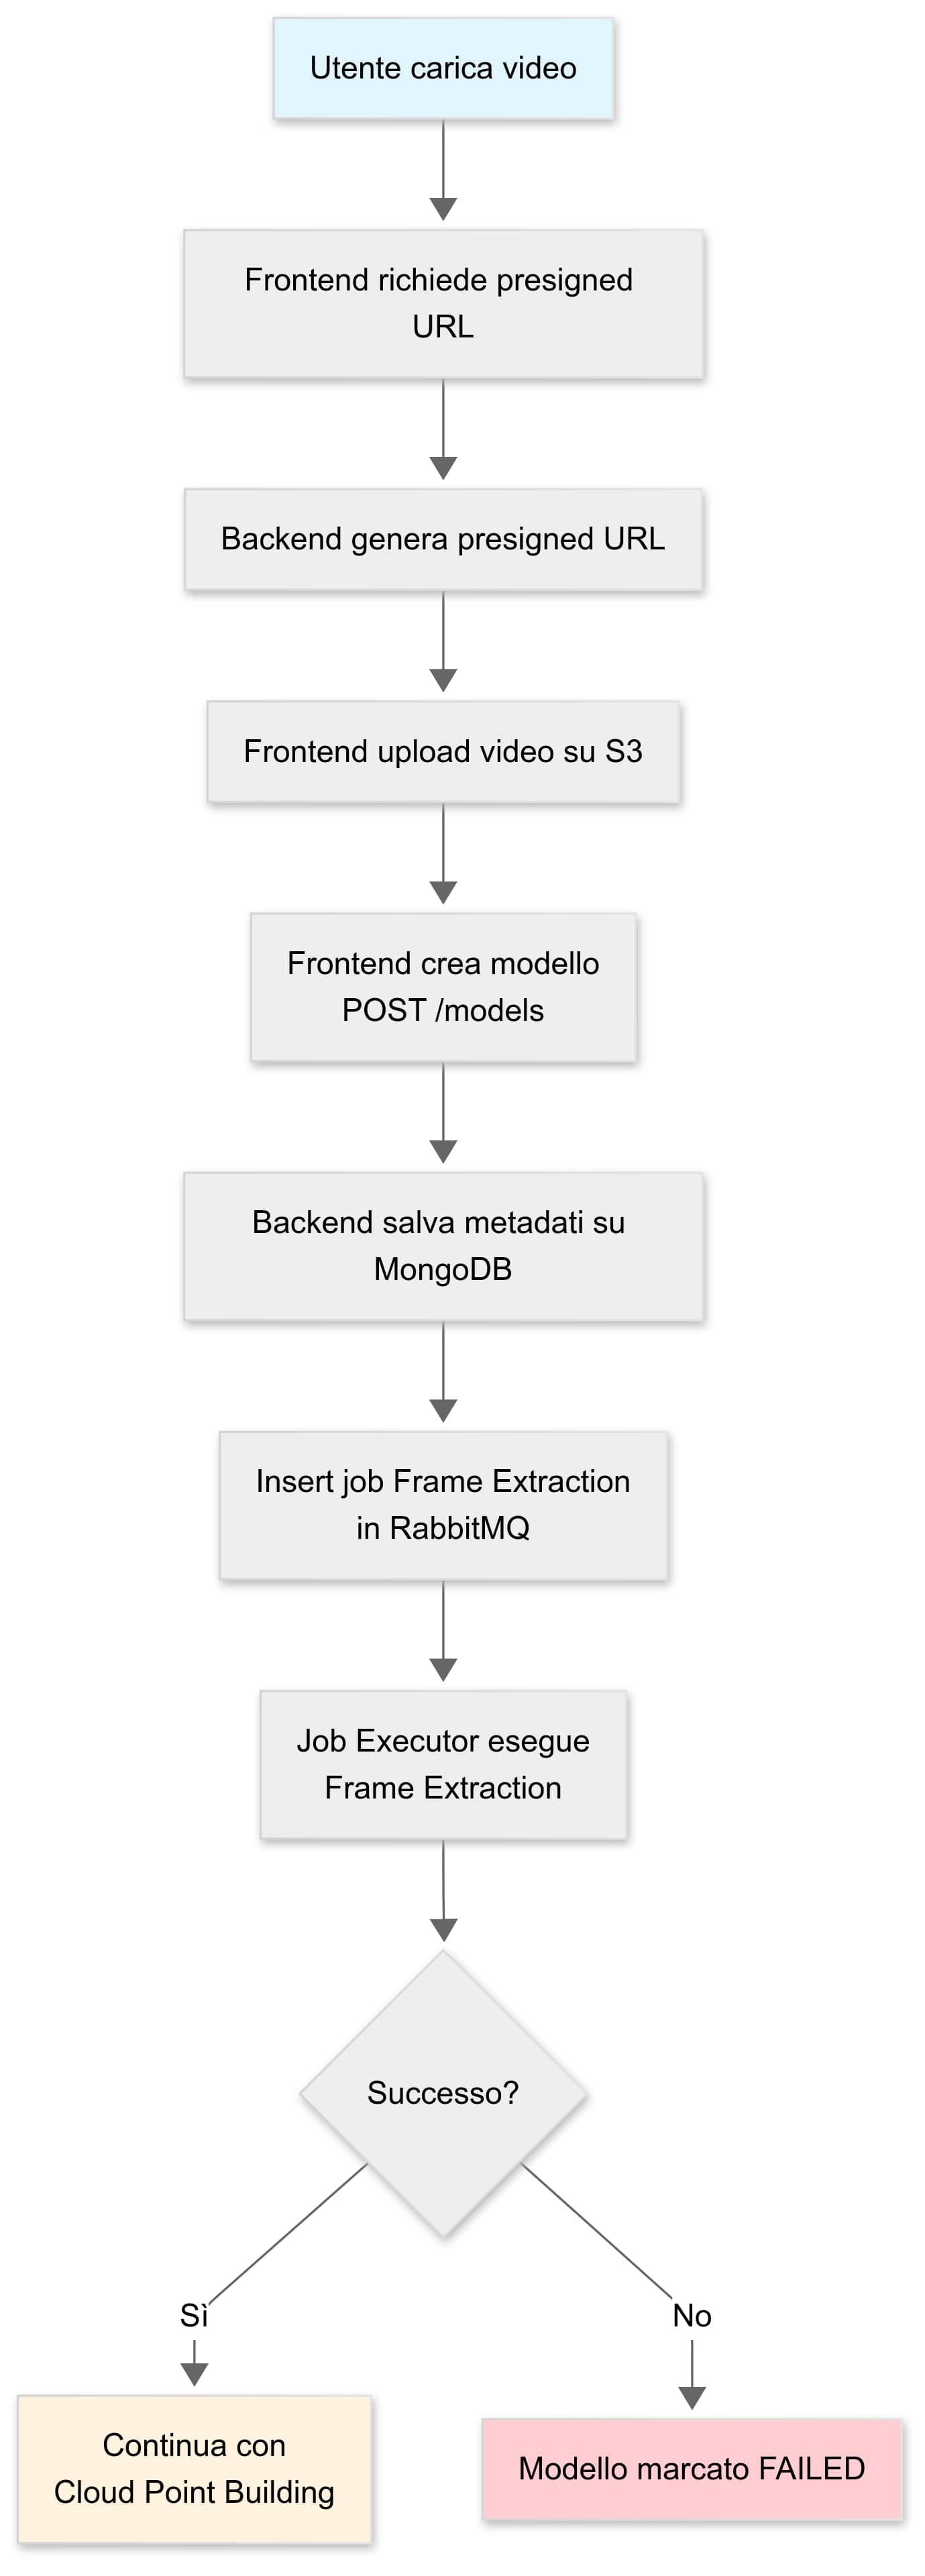
\includegraphics{images/upload_preparazione.jpg}
}
\vspace*{-0.5cm} % Riduci spazio tra figura e didascalia
\caption{Architettura dei componenti del sistema (upload e preprocessing video)}
\label{fig:component_architecture1}
\end{figure}

\begin{figure}[htbp]
\centering
\vspace*{-3cm} % Riduci spazio sopra la figura
\adjustbox{width=0.5\textwidth,center,keepaspectratio}{
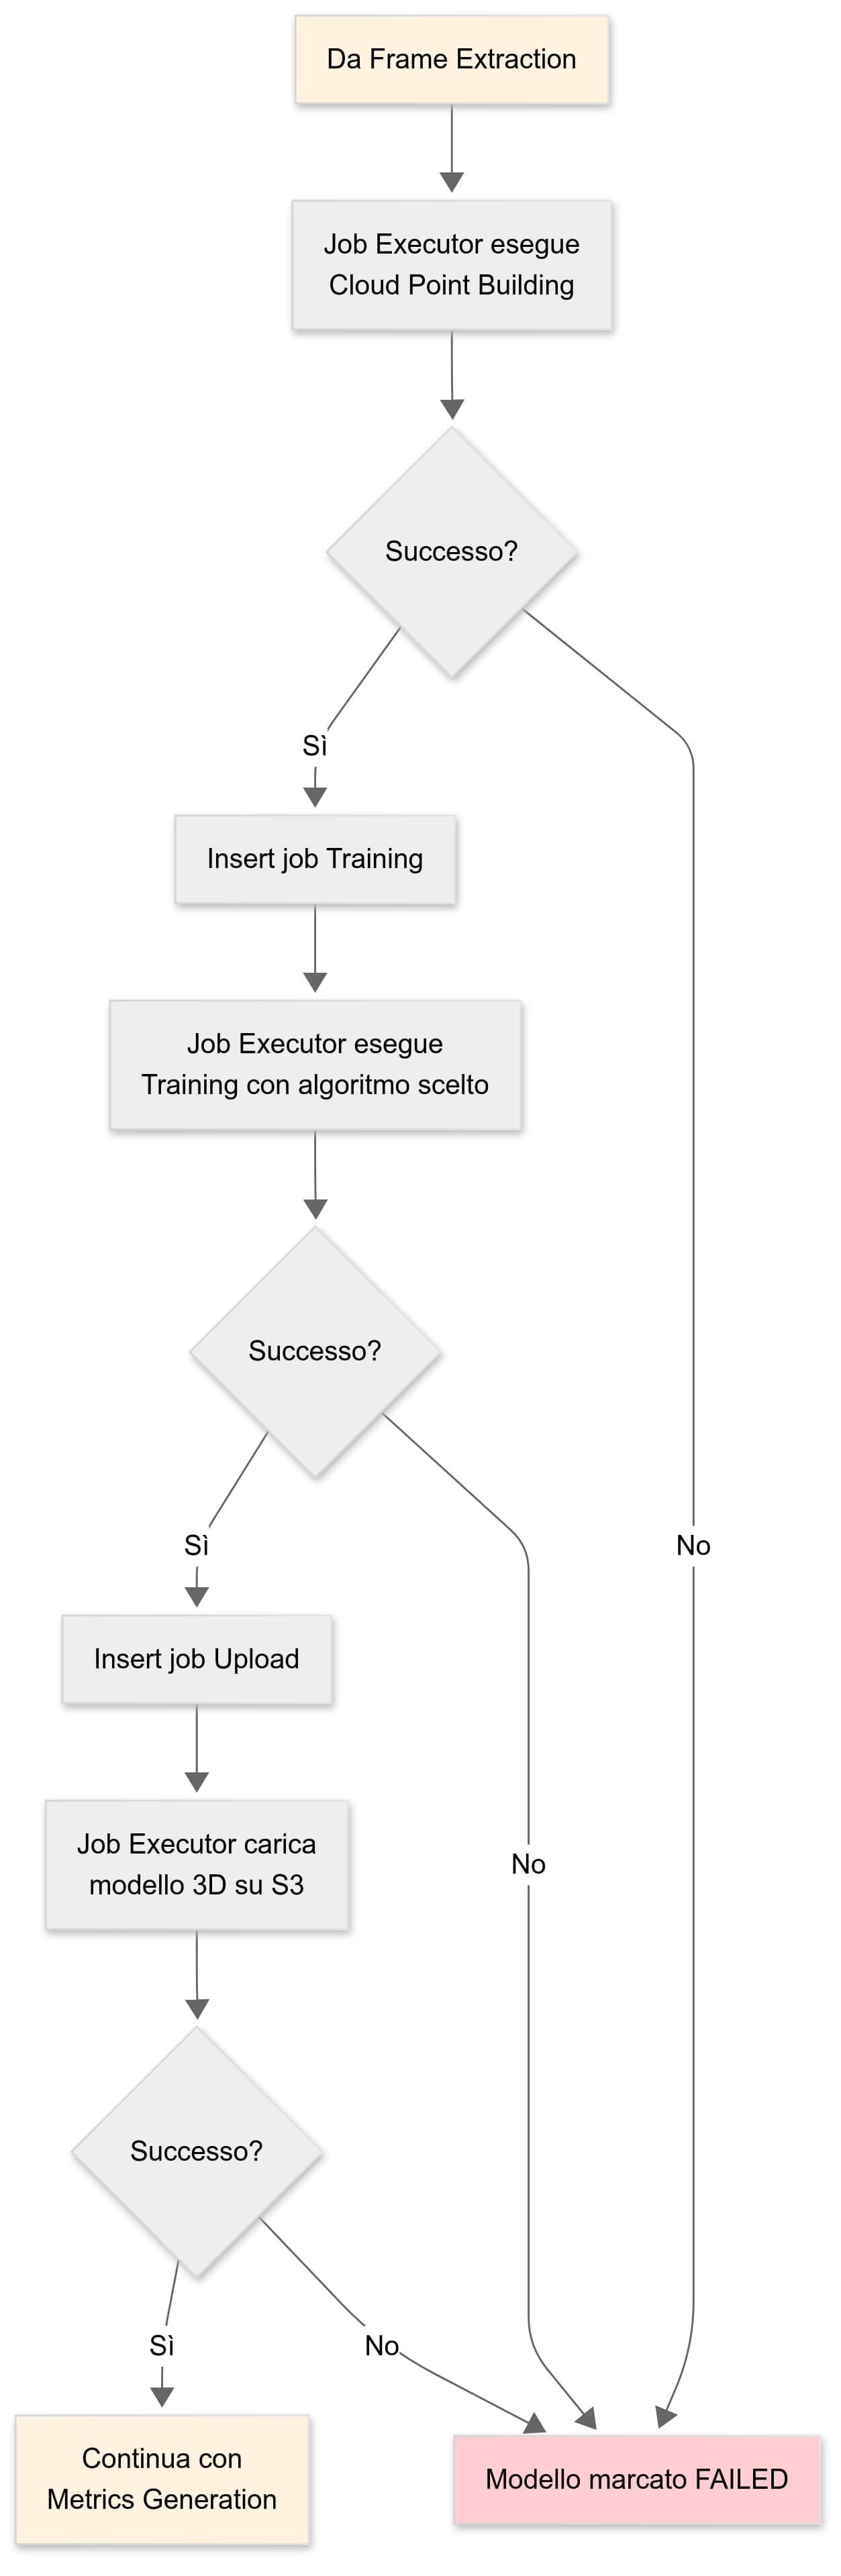
\includegraphics{images/elaborazione_training.jpg}
}
\vspace*{-0.5cm} % Riduci spazio tra figura e didascalia
\caption{Architettura dei componenti del sistema (elaborazione e training)}
\label{fig:component_architecture2}
\end{figure}

\begin{figure}[htbp]
\centering
\vspace*{-1cm} % Riduci spazio sopra la figura
\adjustbox{width=0.6\textwidth,center,keepaspectratio}{
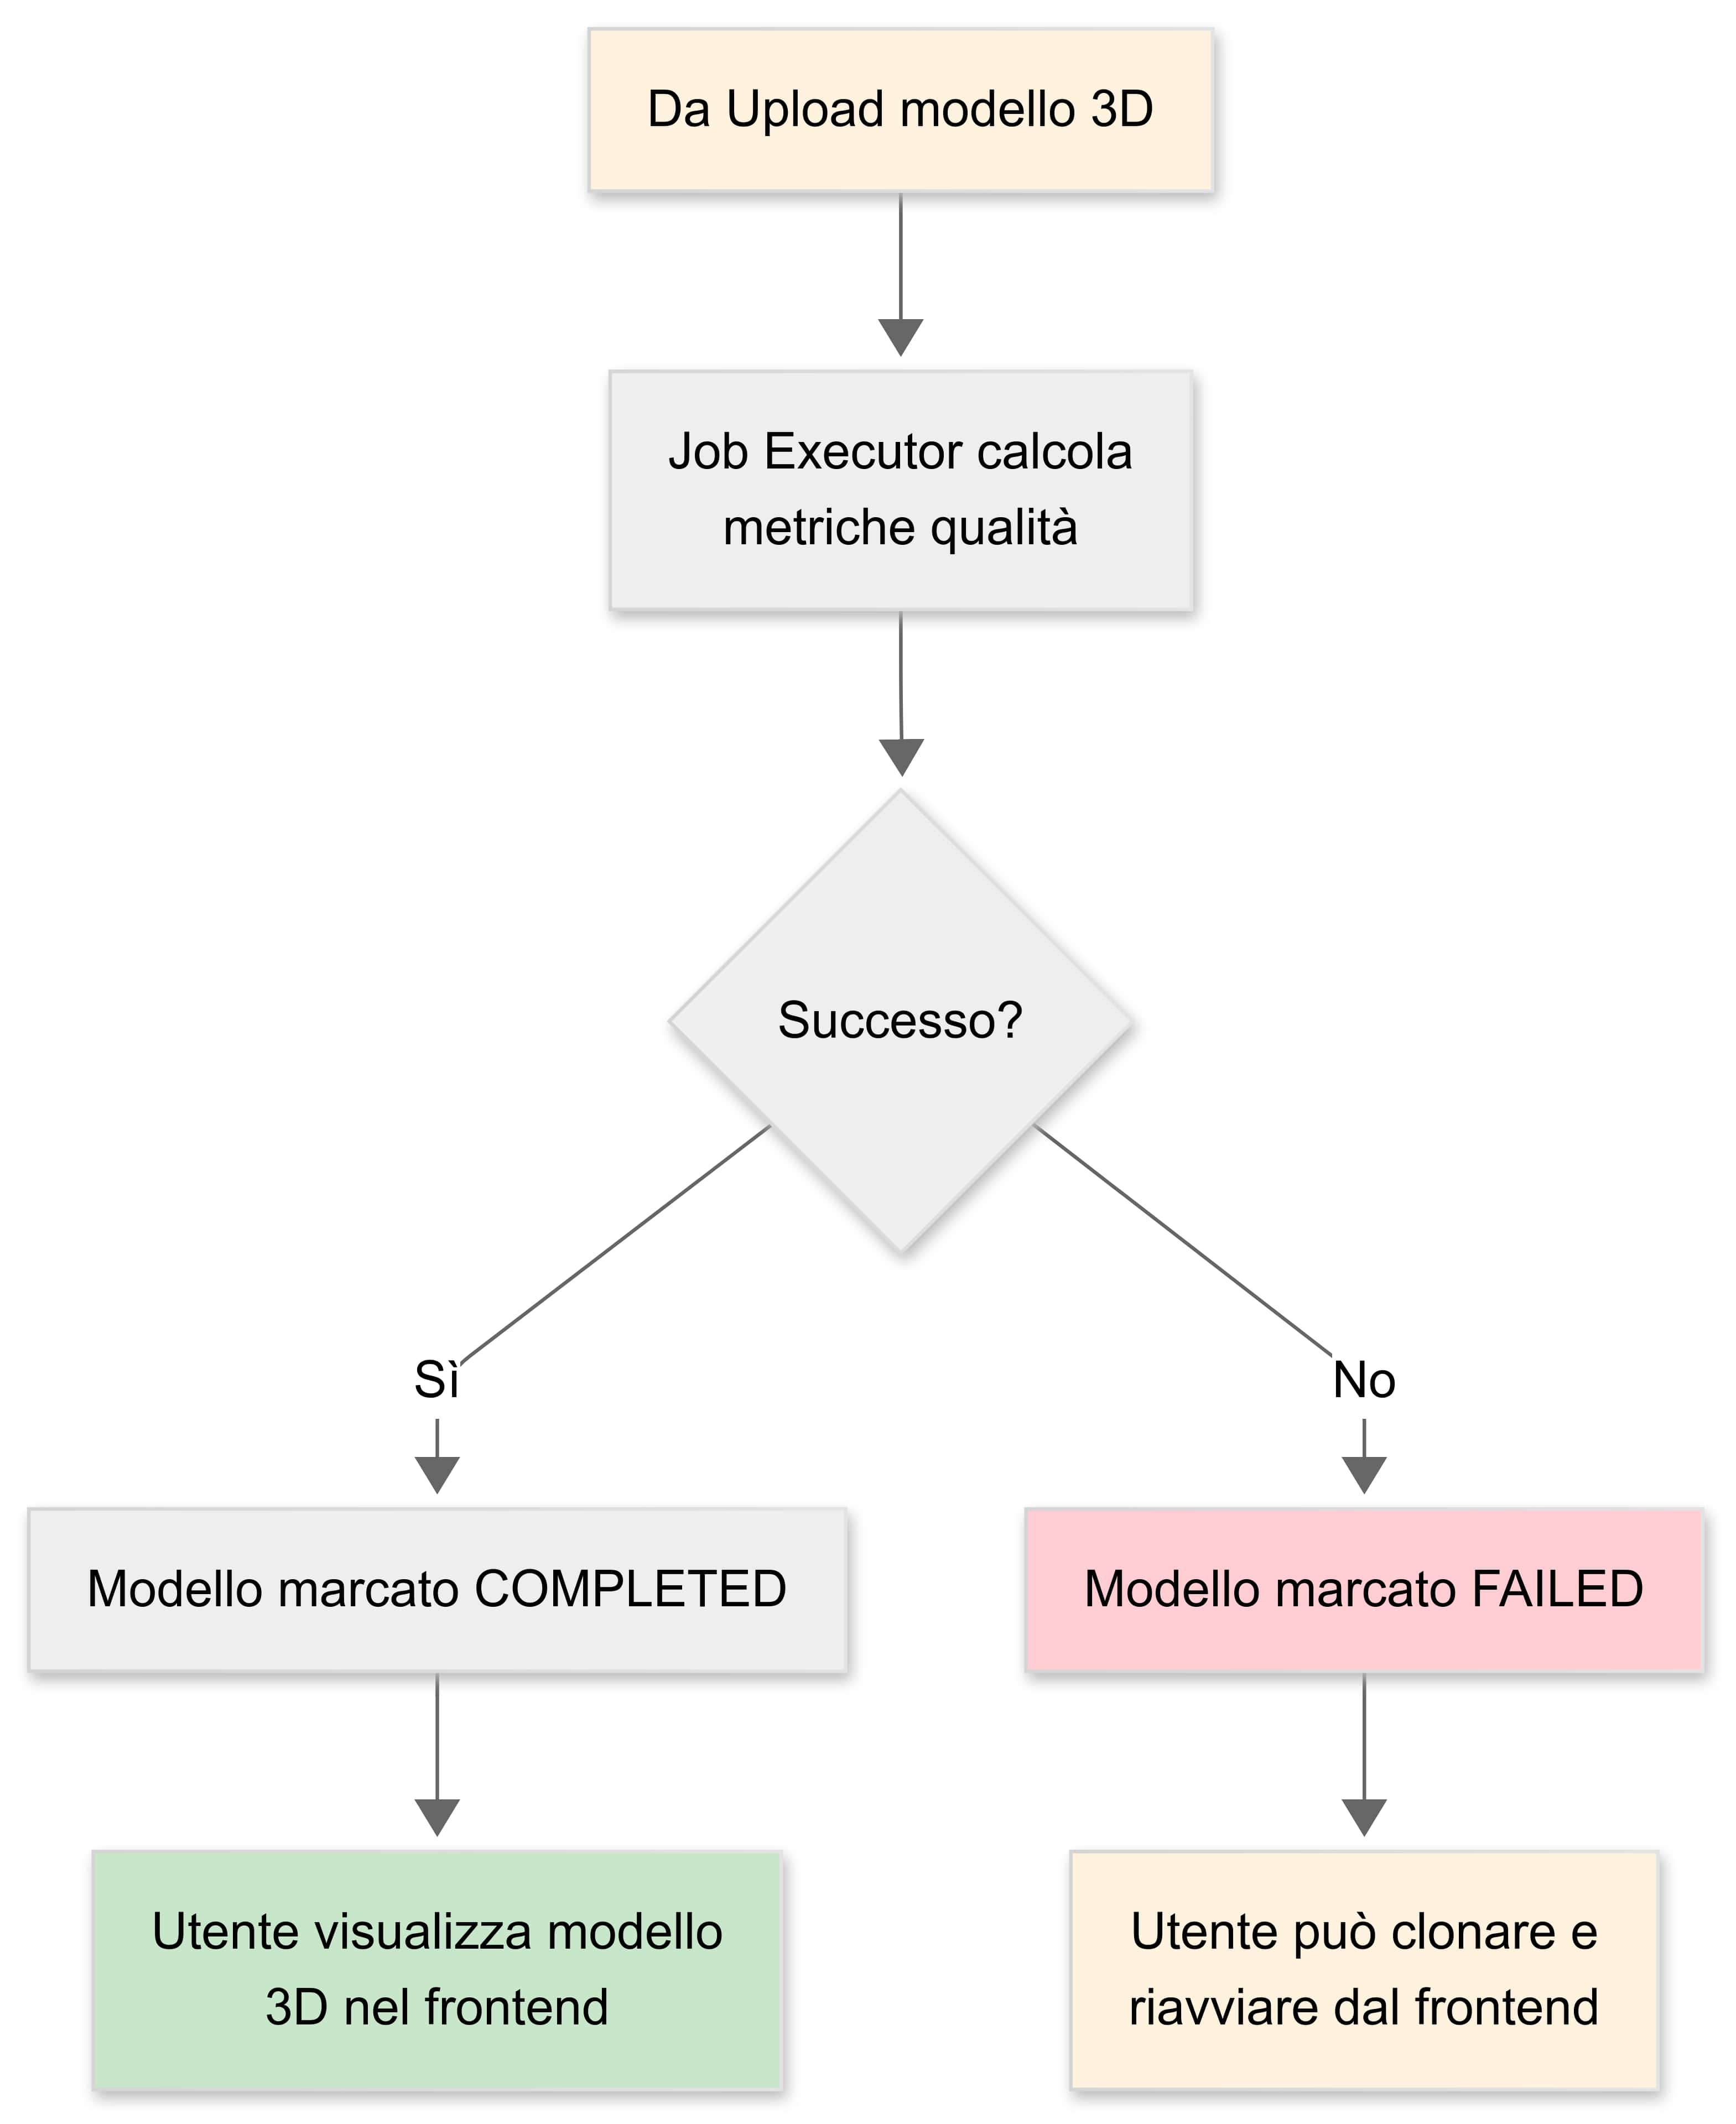
\includegraphics{images/finalizzazione.jpg}
}
\vspace*{-0.5cm} % Riduci spazio tra figura e didascalia
\caption{Architettura dei componenti del sistema (finalizzazione)}
\label{fig:component_architecture}
\end{figure}

\chapter{Implementazioni e tecnologie}
\label{chap:implementazione}

In questo capitolo vengono descritte in dettaglio le scelte tecnologiche e le strategie implementative adottate per la realizzazione del sistema presentato nel Capitolo 2. L’obiettivo principale è offrire una panoramica completa sull’integrazione tra le diverse componenti software e hardware, evidenziando come la combinazione di tecnologie moderne e soluzioni open-source abbia permesso di ottenere un’infrastruttura scalabile, modulare e facilmente manutenibile.

A partire dalla selezione dello stack tecnologico — sia frontend che backend — vengono illustrate le motivazioni alla base delle scelte compiute, le metodologie di containerizzazione e orchestrazione dei servizi, nonché i pattern di persistenza dei dati strutturati e multimediali. Il capitolo approfondisce inoltre i sistemi di parametrizzazione adattiva per l’ottimizzazione delle performance in relazione all’hardware disponibile, le strategie di resilienza, fault tolerance e gestione degli errori implementate per garantire affidabilità operativa anche in contesti distribuiti.

Attraverso una descrizione puntuale dell’implementazione dei singoli layer funzionali — dalla pre-elaborazione del dato grezzo al training degli algoritmi, fino alla visualizzazione interattiva in ambiente web — il lettore potrà apprezzare l’articolazione della soluzione e comprenderne sia gli aspetti di innovazione tecnica, sia i criteri di progettazione orientati alla flessibilità e alla sperimentazione.



\subsection{Stack Tecnologico Implementato}

\subsubsection{Tecnologie Frontend}

Il frontend utilizza \textbf{Vue.js 3} come framework principale per lo sviluppo dell'interfaccia utente, scelto per il bilanciamento tra semplicità e funzionalità. La visualizzazione 3D è implementata attraverso \textbf{GaussianSplats3D}\footnote{\url{https://github.com/mkkellogg/GaussianSplats3D}}, una libreria specializzata basata su \textbf{Three.js} che non supporta, nativamente, il rendering di primitive gaussiane.

\subsubsection{Tecnologie di backend}

Il backend è implementato in \textbf{Python} con \textbf{FastAPI} come framework per le API REST, scelto per le performance superiori e la generazione automatica di documentazione OpenAPI. La gestione asincrona utilizza le capacità native di Python con \textbf{asyncio}.

\subsubsection{Infrastruttura e Persistenza}

L'infrastruttura utilizza \textbf{Docker e Docker Compose} per la containerizzazione e l'orchestrazione locale, \textbf{RabbitMQ} come message broker per la comunicazione asincrona, \textbf{MongoDB} come database NoSQL per metadati, e \textbf{Amazon S3} per lo storage oggetti scalabile.

\subsubsection{Pre-elaborazione specializzata}

I servizi di processing integrano \textbf{COLMAP}\footnote{\url{https://https://colmap.github.io}} per Structure from Motion e per i training services, e \textbf{Sharp Frames}\footnote{\url{https://github.com/Reflct/sharp-frames-python}} per l'estrazione video. Ogni servizio è ottimizzato per l'utilizzo specifico di risorse GPU attraverso configurazioni CUDA dedicate.

L'architettura complessiva garantisce scalabilità, manutenibilità e performance ottimali per l'elaborazione di contenuti 3D, fornendo una base solida per l'implementazione dei componenti specializzati descritti nei capitoli successivi.

\subsubsection{Algoritmi di Training integrati}
Il sistema integra progetti open-source specializzati per il training di rappresentazioni 3D:
\begin{itemize}
	\item \textbf{3D Gaussian Splatting
		for Real-Time Radiance Field Rendering}\footnote{\url{https://github.com/graphdeco-inria/gaussian-splatting}} per la generazione di primitive gaussiane da dataset fotografici
	\item \textbf{3D Gaussian Splatting as Markov Chain Monte Carlo
	}\footnote{\url{https://github.com/ubc-vision/3dgs-mcmc}} con l'introduzione di rumore stocastico nel calcolo dei gradienti
	\item \textbf{Taming 3DGS: High-Quality Radiance Fields with Limited Resources
	}\footnote{\url{https://github.com/ubc-vision/3dgs-mcmc}} per la generazione efficiente di scene 3D con vincoli computazionali ridotti
\end{itemize}
Questi progetti sono stati integrati come servizi containerizzati nel workflow di elaborazione, mantenendo la compatibilità con le implementazioni originali e permettendo aggiornamenti indipendenti.

\subsection{Servizi containerizzati}
\label{sec:servizi_containerizzati}

Per garantire modularità, scalabilità e portabilità del sistema, ciascun componente è stato containerizzato tramite \textbf{Docker}. L'intera infrastruttura si basa su microservizi che comunicano tra loro attraverso una rete virtuale comune, orchestrati da \textbf{Docker Compose}.

Ogni container svolge un ruolo specifico e indipendente nel flusso di elaborazione, riducendo le dipendenze tra i moduli. Di seguito si elencano i principali container e le loro funzioni:

\begin{itemize}
	\item \textbf{Accesso e orchestrazione}
	\begin{itemize}
		\item \textbf{api-gateway}: gestisce il routing delle richieste HTTP verso i microservizi interni.
		\item \textbf{job-executor}: coordina i task tra i moduli e comprende alcune parti di pre e post processing.
	\end{itemize}
	
	\item \textbf{Motori di training e rendering 3D}
	\begin{itemize}
		\item \textbf{gaussian-splatting-api}: esegue il training del Gaussian Splatting 3D e si basa sul paper originale.
		\item \textbf{3dgs-mcmc-api}: esegue il training del Gaussian Splatting 3D con la variante Monte Carlo as Markov Chain.
		\item \textbf{taming-3dgs-api}: motore alternativo di training per scene 3D controllate.
	\end{itemize}
	
	\item \textbf{Pre-elaborazione}
	\begin{itemize}
		\item \textbf{colmap-converter}: wrapper per Colmap, utilizzato per la ricostruzione di point cloud a partire da immagini RGB.
	\end{itemize}
	
	\item \textbf{Persistenza e messaggistica}
	\begin{itemize}
		\item \textbf{mongo}: database NoSQL per la persistenza dei dati.
		\item \textbf{rabbitmq}: message broker per la comunicazione asincrona tra i servizi.
	\end{itemize}
	
	\item \textbf{Visualizzazione}
	\begin{itemize}
		\item \textbf{web-viewer}: interfaccia frontend per l'interazione con il workflow di training e la visualizzazione dei risultati 3D generati.
	\end{itemize}
\end{itemize}

\subsubsection{Esempio di Dockerfile: Gaussian Splatting}
Di seguito è riportato un esempio di \texttt{Dockerfile} utilizzato per il container \texttt{gaussian-splatting}, responsabile del rendering 3D basato su rappresentazioni gaussiane. L'immagine si basa su un container NVIDIA compatibile con CUDA e contiene tutte le dipendenze necessarie per eseguire il motore grafico:

\begin{lstlisting}[language=docker, caption={Dockerfile per gaussian-splatting}, label={lst:dockerfile_gs}]
	FROM nvidia/cuda:12.2.2-cudnn8-devel-ubuntu22.04
	ENV DEBIAN_FRONTEND=noninteractive
	
	# Installazione dipendenze di sistema
	RUN apt update && apt upgrade -y && apt install -y \
	git cmake libxmu-dev libxi-dev libgl-dev libomp-dev \
	python3-dev python3-venv python3-pip build-essential ninja-build wget \
	libboost-program-options-dev libboost-filesystem-dev libboost-graph-dev \
	libboost-system-dev libboost-test-dev libeigen3-dev libflann-dev \
	libfreeimage-dev libmetis-dev libgoogle-glog-dev libgflags-dev \
	libsqlite3-dev libglew-dev qtbase5-dev libqt5opengl5-dev libcgal-dev \
	gcc-10 g++-10 libatlas-base-dev libsuitesparse-dev
	
	# Clonazione del repository
	WORKDIR /workspace
	RUN git clone https://github.com/graphdeco-inria/gaussian-splatting --recursive
	
	# Installazione dipendenze Python
	COPY requirements.txt /workspace/gaussian-splatting/
	WORKDIR /workspace/gaussian-splatting
	RUN pip3 install --upgrade pip && \
	pip3 install torch torchvision --extra-index-url https://download.pytorch.org/whl/cu121 && \
	pip3 install -r requirements.txt
	
	# Compilazione moduli C++
	RUN cd submodules/diff-gaussian-rasterization && pip3 install .
	RUN cd submodules/simple-knn && pip3 install .
	RUN cd submodules/fused-ssim && pip3 install .
	
	# Supporto Depth Anything V2
	WORKDIR /workspace
	RUN git clone https://github.com/DepthAnything/Depth-Anything-V2.git
	WORKDIR /workspace/Depth-Anything-V2
	RUN pip3 install opencv-python transformers pillow numpy matplotlib
	RUN mkdir -p checkpoints && \
	wget -O checkpoints/depth_anything_v2_vitl.pth \
	https://huggingface.co/depth-anything/Depth-Anything-V2-Large/resolve/main/depth_anything_v2_vitl.pth
	
	# Ritorno alla directory principale
	WORKDIR /workspace/gaussian-splatting
	CMD ["bash"]
\end{lstlisting}

In seguito, viene definita un'estensione del container per esporre un'interfaccia \texttt{FastAPI}, utile per l'interazione RESTful con il modulo computazionale:

\begin{lstlisting}[language=docker, caption={Estensione API FastAPI per Gaussian Splatting}, label={lst:dockerfile_api}]
	FROM gaussian-splatting
	
	ARG API_PORT=8100
	ENV API_PORT=$API_PORT
	EXPOSE $API_PORT
	
	WORKDIR /workspace/gaussian-splatting
	COPY api.py /workspace/gaussian-splatting/api.py
	
	RUN mkdir -p /tmp/runtime-root && chmod 0700 /tmp/runtime-root
	ENV QT_QPA_PLATFORM=offscreen
	ENV PYTHONUNBUFFERED=1
	
	RUN pip3 install fastapi uvicorn
	
	CMD ["/bin/bash", "-c", "uvicorn api:app --host 0.0.0.0 --port $API_PORT"]
\end{lstlisting}

Questa struttura modulare consente di disaccoppiare il motore grafico dall’interfaccia espositiva, migliorando la manutenibilità e favorendo l’integrazione in pipeline distribuite.
\newpage
\section{Sistema di parametrizzazione adattiva per livelli di qualità e auto-scaling hardware}

Il workflow implementa un sistema di parametrizzazione multi-livello progettato per bilanciare qualità dell'output e vincoli hardware, provando a garantire sempre la generazione di un modello 3D indipendentemente dalle limitazioni del sistema. Tale parametrizzazione cerca di far coesistere i seguenti aspetti:

\begin{itemize}
	\item \textbf{Livelli di qualità utente}: l'utente può scegliere tra tre preset (Fast, Balanced, Quality) che influenzano parametri critici come risoluzione target, numero di frame estratti, iterazioni di training e soglie di densificazione. Questa scelta rappresenta l'\textbf{intento} di qualità desiderato, ma non è vincolante per l'esecuzione.
	
	\item \textbf{Hardware adaptation e graceful degradation}: il sistema, tramite il TrainingParamsService, rileva la VRAM disponibile e applica un downscaling conservativo dei parametri critici (risoluzione, batch size, frame count, ecc.). Questo approccio di graceful degradation è implementato solo in fase di setup: il sistema preferisce ridurre preventivamente la qualità dell’output per prevenire errori di esaurimento risorse (OOM) o crash del container. Una volta avviato il workflow, non sono previsti adattamenti dinamici.

\end{itemize}

\subsection{Struttura dei parametri}

La configurazione di ogni algoritmo è organizzata in categorie distinte, ciascuna con uno scopo specifico nel workflow:

\begin{itemize}
\item \textbf{\texttt{base\_params}}: definiscono i valori di partenza dell'algoritmo, tipicamente corrispondenti ai parametri di default della implementazione originale. Rappresentano la base dalla quale vengono costruiti tutti e tre i livelli di qualità attraverso l'applicazione dei moltiplicatori. Questi parametri influenzano direttamente il comportamento degli algoritmi di training (numero di iterazioni, soglie di densificazione, intervalli di ottimizzazione).

\item \textbf{\texttt{quality\_multipliers}}: moltiplicatori che vengono applicati esclusivamente ai \texttt{base\allowbreak\_params} per generare i parametri finali di training per ciascun livello di qualità. Il livello "fast" riduce tipicamente le iterazioni e accelera il processo, mentre "quality" incrementa la precisione computazionale a scapito dei tempi di elaborazione.

\item \textbf{\texttt{preprocessing\_params}}: parametri che influenzano esclusivamente la fase di preprocessing (estrazione frame, ridimensionamento video) e che non vengono passati agli algoritmi di training. Include risoluzione target e numero di frame da estrarre, parametri che impattano sulla qualità del dataset di input ma rimangono esterni alla logica di training.

\item \textbf{\texttt{manual\_overrides}}: parametri opzionali che possono essere specificati manualmente dall’utente (o dal chiamante API) per forzare valori di training specifici. Gli override hanno priorità su qualsiasi altro parametro calcolato o derivato dai preset, adattamenti hardware e moltiplicatori di qualità. 

\item \textbf{\texttt{hardware\_config}}: definisce le soglie VRAM e le formule di scaling automatico. I \texttt{resolution\_thresholds} stabiliscono le risoluzioni massime supportate per ogni configurazione hardware, le \texttt{scaling\_formulas} permettono un adattamento dinamico dei parametri di training in base alla memoria disponibile.
\end{itemize}


\subsection{Processo di Calcolo Parametri}

Il \texttt{TrainingParamsService} implementa una pipeline di calcolo che trasforma le configurazioni di base in parametri finali pronti per l'esecuzione:

\begin{figure}[htbp]
	\centering
	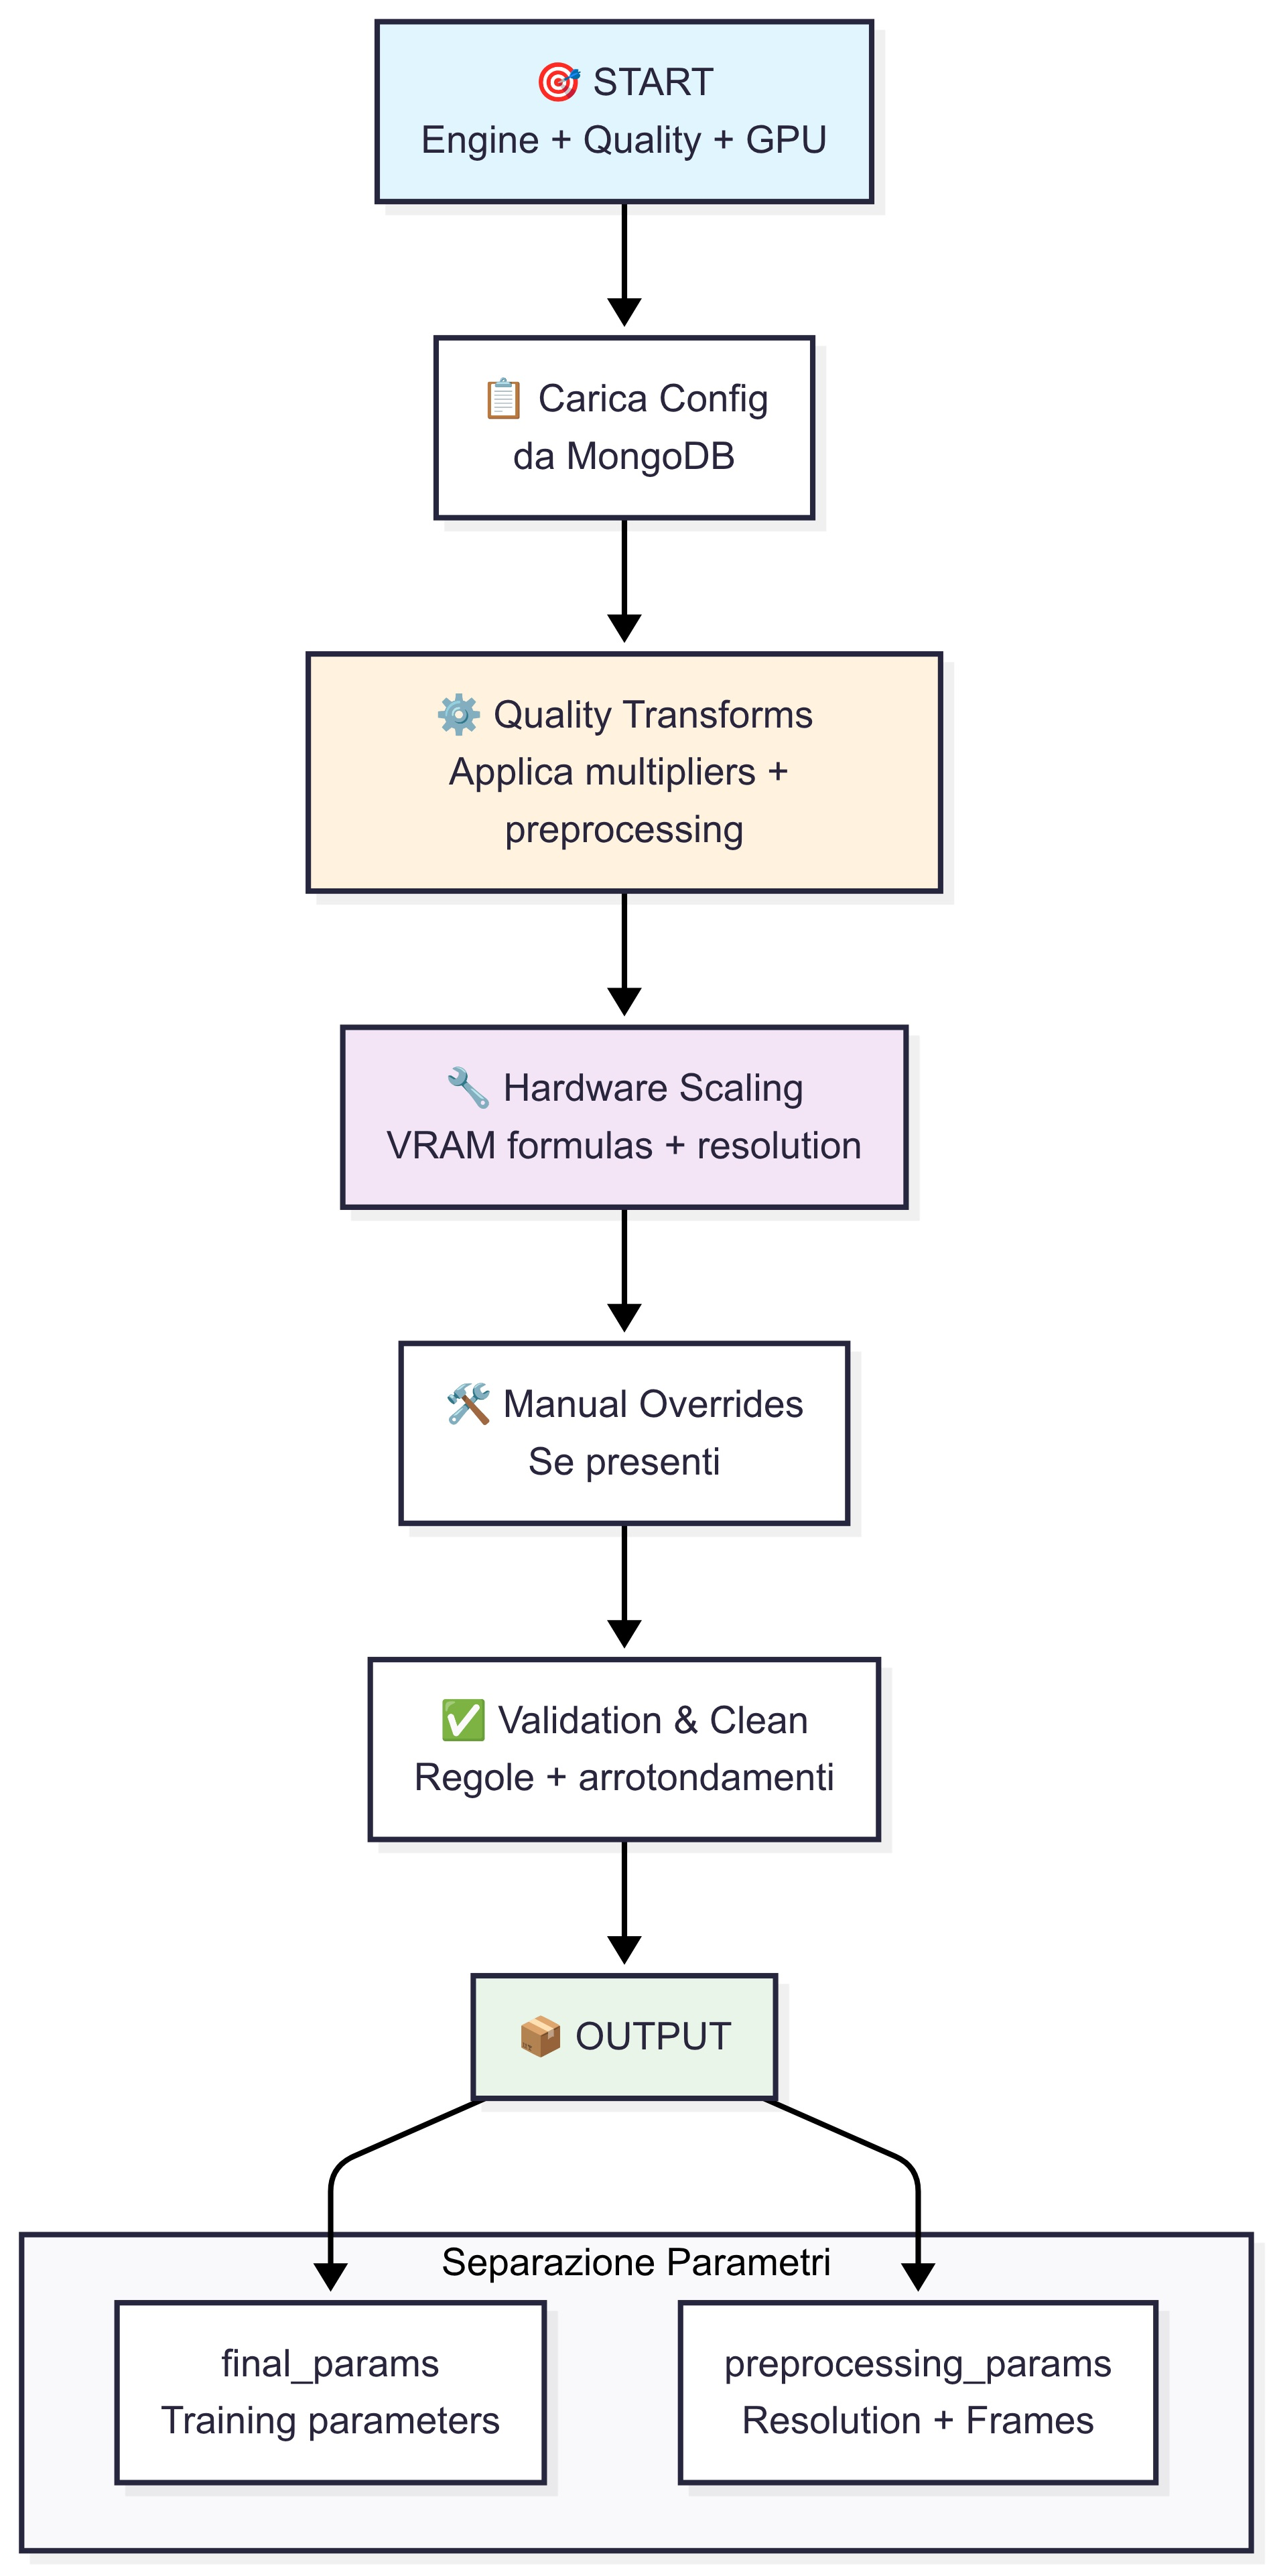
\includegraphics[width=0.7\textwidth]{images/training_params_service_workflow.jpg}
	\caption{Workflow della generazione dei parametri adattivi}
	\label{fig:training_params_service_workflow}
\end{figure}

La separazione netta tra parametri di training e preprocessing consente al sistema di adattare indipendentemente la qualità del dataset di input (risoluzione, numero di frame) e la precisione computazionale del training, ottimizzando l'utilizzo delle risorse hardware disponibili.

\subsection{Configurabilità e Sperimentazione}

Un aspetto fondamentale dell'architettura è la \textbf{persistenza delle configurazioni in MongoDB}, che offre all'owner dell'applicazione la possibilità di modificare dinamicamente i parametri senza dover ricompilare o ridistribuire il software. Questa caratteristica è particolarmente vantaggiosa per:

\begin{itemize}
	\item \textbf{Ottimizzazione empirica}: L'owner può testare diverse combinazioni di parametri, moltiplicatori di qualità e soglie hardware per trovare il bilanciamento ottimale tra qualità dell'output e performance del sistema. Le modifiche alle configurazioni diventano immediatamente operative per tutti i nuovi job.
	
	\item \textbf{Adattamento hardware-specifico}: Ogni deployment può essere fine-tuned per l'hardware specifico disponibile, le \texttt{resolution\_thresholds} e le \texttt{scaling\_formulas} vengono modificate in base alle caratteristiche delle GPU installate e ai risultati dei test empirici.
	
	\item \textbf{Evoluzione degli algoritmi}: L'aggiunta di nuovi algoritmi o l'aggiornamento di quelli esistenti richiede solamente l'inserimento di un nuovo documento nella collection \texttt{training\_params}, mantenendo la retrocompatibilità con il codice esistente.
\end{itemize}

Questa flessibilità consente un approccio iterativo al miglioramento delle performance, dove l'esperienza operativa può guidare l'evoluzione delle configurazioni verso setup sempre più ottimizzati per il contesto di deployment specifico.

\section{Layer di Storage}

Il layer di storage è implementato seguendo una strategia di persistenza ibrida che combina MongoDB per i metadati strutturati e Amazon S3 per lo storage di contenuti multimediali e modelli 3D. Questa architettura ottimizza l'accesso ai dati in base ai pattern di utilizzo specifici di ogni tipo di informazione.

\subsection{MongoDB - Database dei metadati}

MongoDB è configurato come replica set per garantire consistenza e supportare operazioni di change stream necessarie per le notifiche real-time.
Il database è organizzato in tre collection principali, ciascuna ottimizzata per specifici pattern di accesso:

\subsubsection{Collection "models"}
La collection principale memorizza i metadati dei modelli 3D e il tracking delle fasi di elaborazione:

\begin{lstlisting}[language=javascript, caption=Struttura documento modello]
	{
		"_id": "ObjectId",
		"model_name": "Video Demo 1",
		"created_at": "2024-07-24T10:30:00Z",
		"video_s3_key": "videos/uuid-123/input_video.mp4",
		"zip_model_suffix": "3d_model.zip",
		"overall_status": "COMPLETED",
		"current_phase": "metrics_evaluation",
		"parent_model_id": null,  // Per supportare la fork
		
		// Tracking dettagliato delle fasi
		"phases": {
			"frame_extraction": {
				"status": "COMPLETED",
				"started_at": "2024-07-24T10:30:00Z",
				"completed_at": "2024-07-24T10:32:00Z",
				"metadata": {
					"frame_count": 180,
					"processing_params": {"fps": 6, "width": 1920}
				}
			},
			"training": {
				"status": "COMPLETED",
				"metadata": {
					"training_duration_seconds": 1847.3,
					"training_parameters": {
						"engine": "INRIA",
						"quality_level": "balanced",
						"final_params": {"iterations": 30000, "lr": 0.0025}
					}
				}
			},
			"metrics_evaluation": {
				"status": "COMPLETED",
				"metadata": {
					"metrics": {
						"PSNR": 28.45,
						"SSIM": 0.89,
						"LPIPS": 0.12
					}
				}
			}
		},
		
		// Configurazione training
		"training_config": {
			"engine": "INRIA",
			"quality_level": "balanced"
		}
	}
\end{lstlisting}

\textbf{Motivazioni del design}:
\begin{itemize}
	\item \textbf{Struttura denormalizzata}: Le fasi sono embedded nel documento per ridurre le query multiple
	\item \textbf{Metadati flessibili}: Schema dinamico per adattarsi ai diversi tipi di informazioni per fase
	\item \textbf{Supporto fork}: Il campo \texttt{parent\_model\_id} abilita la creazione di varianti (fork)
	\item \textbf{Tracking temporale}: Timestamp dettagliati per analisi performance e debugging
\end{itemize}

\subsubsection{Collection \texttt{"training\_params"}}
Memorizza le configurazioni degli algoritmi con parametrizzazione multi-livello:

\begin{lstlisting}[language=javascript, caption=Struttura configurazione algoritmo]
	{
		"algorithm_name": "gaussian_splatting_original",
		"display_name": "3D Gaussian Splatting (Fixed Iterations)",
		"version": "1.5",
		"active": true,
		
		// Parametri base (livello balanced)
		"base_params": {
			"iterations": 30000,
			"densify_grad_threshold": 0.0002,
			"densification_interval": 100,
			"eval": true
		},
		
		// Moltiplicatori per livelli di qualità
		"quality_multipliers": {
			"fast": {"iterations": 0.8, "densify_grad_threshold": 1.2},
			"balanced": {"iterations": 1.0, "densify_grad_threshold": 1.0},
			"quality": {"iterations": 1.2, "densify_grad_threshold": 0.8}
		},
		
		// Configurazione hardware-specific
		"hardware_config": {
			"baseline_vram_gb": 24,
			"min_vram_gb": 8,
			"resolution_thresholds": [
			{"vram_threshold": 24, "target_width": 3840, "target_height": 2160},
			{"vram_threshold": 16, "target_width": 1920, "target_height": 1080}
			],
			"scaling_formulas": {
				"densify_grad_threshold": {
					"formula": "max(1.0, 2.5 - (vram_factor * 1.5))",
					"min": 1.0, "max": 4.0
				}
			}
		}
	}
\end{lstlisting}
\newpage
\textbf{Vantaggi dell'approccio}:
\begin{itemize}
	\item \textbf{Configurabilità runtime}: Modifiche ai parametri senza redeploy
	\item \textbf{Sperimentazione facilitata}: Test di configurazioni diverse per ottimizzazioni
	\item \textbf{Adattamento hardware}: Scaling automatico basato su VRAM disponibile
	\item \textbf{Versionamento}: Tracking delle evoluzioni delle configurazioni
\end{itemize}

\subsubsection{Collection \texttt{"users"}}
Sistema di autenticazione con ruoli e gestione sessioni:

\begin{lstlisting}[language=javascript, caption=Struttura utente]
	{
		"_id": "ObjectId",
		"username": "admin",
		"hashed_password": "$2b$12$...",  // bcrypt hash
		"role": "admin",
		"created_at": "2024-07-24T10:00:00Z",
		"last_login": "2024-07-24T15:30:00Z"
	}
\end{lstlisting}

\subsection{Amazon S3 - Object Storage}

\subsubsection{Organizzazione Bucket e Prefissi}

Il sistema utilizza una strategia di organizzazione gerarchica su S3 per ottimizzare l'accesso e la gestione del ciclo di vita dei contenuti:
\newline
\dirtree{%
	.1 s3://3dgs-bucket/.
	.2 videos/.
	.3 \{model\_id\}/.
	.4 input\_video.mp4.
	.2 delivery/.
	.3 \{model\_id\}/.
	.4 3d\_model.zip.
	.2 staging/.
	.3 \{model\_id\}/.
	.4 phase\_frame\_extraction.zip.
	.4 point\_cloud\_building\_phase.zip.
	.4 training\_phase.zip.
}

\subsubsection{Gestione contenuti per tipologia}

\paragraph{Video sorgente (videos/)}
I video originali caricati dagli utenti vengono memorizzati con chiavi UUID per evitare conflitti e garantire privacy:

\begin{lstlisting}[language=python, caption=Generazione chiave video]
	upload_id = str(uuid4())
	s3_key = f"videos/{upload_id}/input_video.mp4"
	presigned_url = repository_service.generate_presigned_url_upload(s3_key, content_type)
\end{lstlisting}

\textbf{Caratteristiche}:
\begin{itemize}
	\item \textbf{Upload diretto}: Utilizzo di presigned URL per evitare transito attraverso backend
	\item \textbf{Retention policy}: Possibile archiviazione automatica dopo completamento processing
	\item \textbf{Versioning}: Supporto per multiple versioni dello stesso contenuto
\end{itemize}

\paragraph{Modelli finali (delivery/)}
I modelli 3D ottimizzati per la visualizzazione web vengono memorizzati in formato compresso ed ogni archivio contiene la cloud point finale in formato .ksplat e la lista delle camere in formato .json prodotte dall'algoritmo di training:

\begin{lstlisting}[language=python, caption=Upload modello finale]
	zip_model_s3_key = f"delivery/{model_id}/3d_model.zip"
	# Contiene: point_cloud.ksplat + cameras.json
	repository_service.upload(zip_filename, zip_model_s3_key)
\end{lstlisting}

\textbf{Ottimizzazioni}:
\begin{itemize}
	\item \textbf{Formato KSPLAT}: Conversione da PLY per ridurre dimensioni e ottimizzare rendering
	\item \textbf{CDN integration}: Possibile distribuzione attraverso CloudFront per performance globali
	\item \textbf{Caching headers}: Configurazione per ottimizzare caching browser
\end{itemize}

\paragraph{Dati Intermedi (staging/)}
Le fasi intermedie vengono persistite per supportare fork, retry e debugging:

\begin{lstlisting}[language=python, caption=Pattern salvataggio fase intermedia]
	phase_zip_s3_key = f"staging/{parent_model_id}/{PHASE_NAME}_phase.zip"
	phase_zip_helper.create_phase_zip_and_upload(model_id, model_dir, PHASE_NAME, directories)
\end{lstlisting}

\textbf{Benefici}:
\begin{itemize}
	\item \textbf{Recuperabilità}: Possibilità di ripartire da fasi intermedie in caso di errori
	\item \textbf{Sperimentazione}: Fork di modelli per testare algoritmi diversi senza reprocessing completo
	\item \textbf{Debugging}: Accesso ai dati intermedi per analisi e ottimizzazioni
\end{itemize}

\subsubsection{Pattern di Accesso Ottimizzati}

\paragraph{Workflow di elaborazione}
Durante l'elaborazione, il sistema implementa un pattern cache-first per ottimizzare l'I/O:

\begin{lstlisting}[language=python, caption=Pattern cache-first per dati S3]
	# 1. Verifica cache locale
	if os.path.exists(local_cache_path) and is_valid_cache(local_cache_path):
	return local_cache_path
	
	# 2. Download da S3 con caching
	repository_service.download(s3_key, local_path)
	update_cache_metadata(local_path)
	return local_path
\end{lstlisting}
\newpage
\paragraph{Frontend Access Pattern}
Per l'accesso frontend, il sistema combina metadata queries su MongoDB con contenuti diretti da S3:

\begin{lstlisting}[language=python, caption=Pattern accesso ibrido frontend]
	# 1. Recupera metadati da MongoDB
	model_metadata = model_service.get_model_by_id(model_id)
	
	# 2. Genera URL diretto per contenuti S3
	if model_metadata.zip_model_suffix:
	model_url = f"https://s3.amazonaws.com/bucket/delivery/{model_id}/{model_metadata.zip_model_suffix}"
	
	return {
		"metadata": model_metadata,
		"model_download_url": model_url
	}
\end{lstlisting}

Questa strategia ibrida garantisce performance ottimali combinando la flessibilità di MongoDB per query complesse sui metadati con la scalabilità e durabilità di S3 per contenuti di grandi dimensioni.

\section{Layer di Orchestrazione}
Il layer di orchestrazione coordina in modo asincrono l'esecuzione sequenziale delle cinque fasi di elaborazione del workflow. L'implementazione si basa su RabbitMQ come message broker e implementa un pattern Producer-Consumer specializzato per gestire workflow di training complessi con supporto per operazioni di retry e fork.

\subsection{Code di messaggi e configurazione RabbitMQ}

Il sistema implementa cinque code dedicate, ciascuna responsabile di una fase specifica del workflow:

\begin{lstlisting}[language=python, caption=Definizione code specializzate per workflow]
	queues = [
	'frame_extraction_queue',      # Fase 1: Estrazione frame video
	'point_cloud_queue',           # Fase 2: Generazione nuvola punti  
	'model_training_queue',        # Fase 3: Training algoritmi GS
	'upload_queue',                # Fase 4: Upload modello 3D
	'metrics_generation_queue'     # Fase 5: Calcolo metriche qualità
	]
\end{lstlisting}

\subsubsection{Configurazione di persistenza e acknowledgment}

Ogni coda è configurata per garantire la massima affidabilità del sistema:

\begin{itemize}
	\item \textbf{Persistenza delle code}: \texttt{durable=True} garantisce che le code sopravvivano ai riavvii del broker
	\item \textbf{Persistenza dei messaggi}: \texttt{delivery\_mode=2} assicura che tutti i messaggi siano scritti su disco
	\item \textbf{Acknowledgment immediato}: I messaggi RabbitMQ vengono consumati e confermati immediatamente dopo la lettura e il parsing, prima dell'avvio del job vero e proprio. Questo garantisce che i messaggi non rimangano bloccati in coda in caso di problemi durante l'elaborazione e permette di interrompere definitivamente job problematici tramite il restart dei container, senza che questi vengano automaticamente riprocessati.
\end{itemize}

\subsubsection{Monitoraggio RabbitMQ}

Il sistema fornisce visibilità completa attraverso la RabbitMQ Management Interface, che offre monitoraggio real-time delle code, includendo:

\begin{itemize}
	\item Numero di messaggi in attesa per ogni coda
	\item Throughput e metriche di performance
	\item Stato delle connessioni producer-consumer
	\item Gestione delle connessioni dedicate e isolate tra API Gateway (producer) e Job Executor (consumer)
\end{itemize}

\begin{figure}[h]
	\centering
	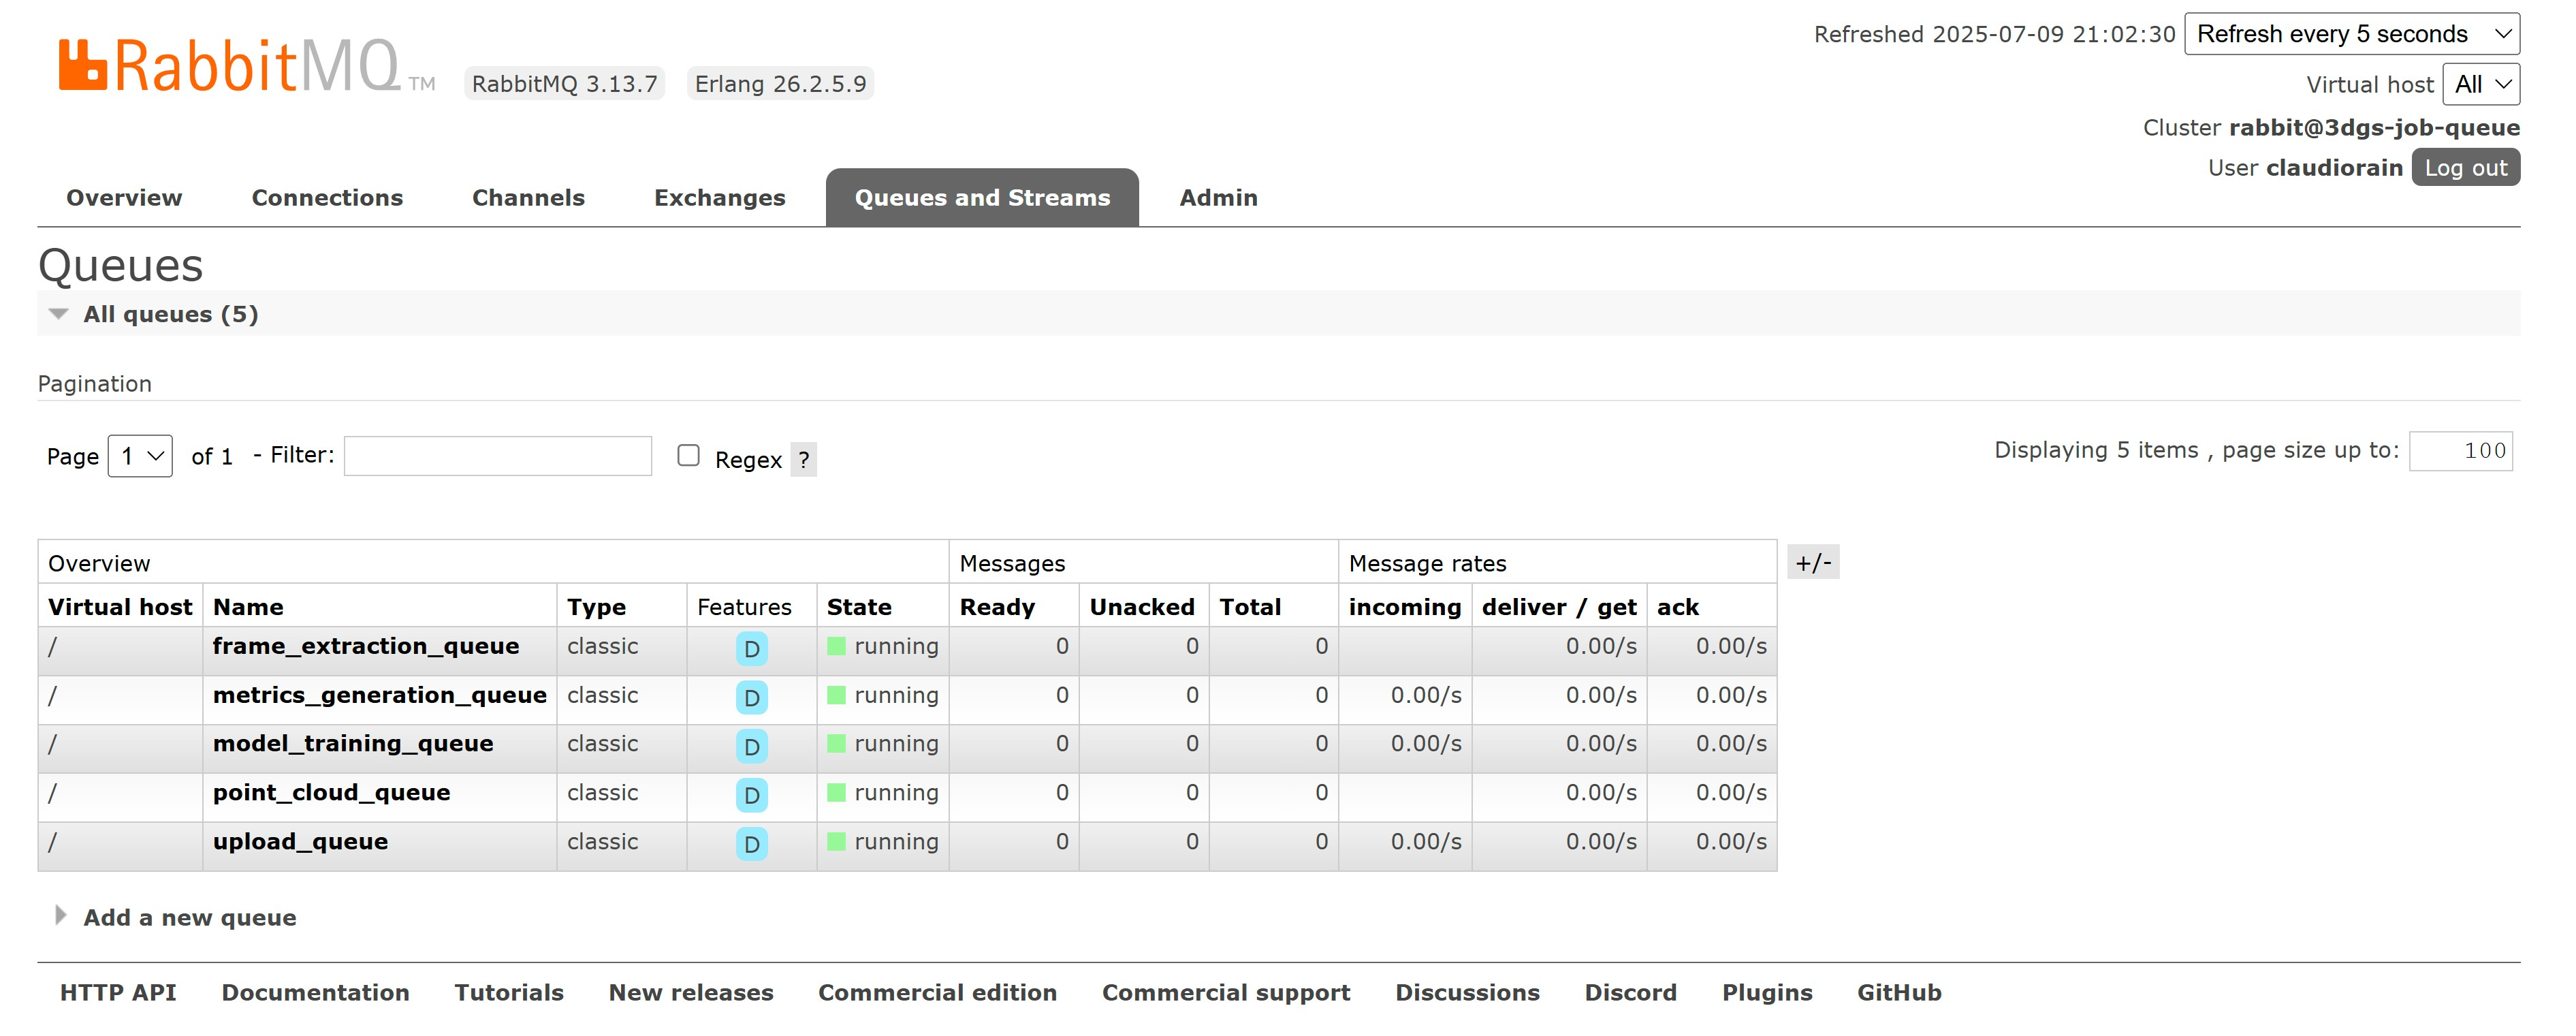
\includegraphics[width=\textwidth]{images/rabbitmq_queues_interface.jpg}
	\caption{Interfaccia di gestione RabbitMQ - Vista code attive del sistema}
	\label{fig:rabbitmq_queues}
\end{figure}

\subsection{Pattern Producer-Consumer ibrido}

Il sistema implementa una variante specializzata del pattern Producer-Consumer tradizionale, dove il Job Executor assume alternativamente i ruoli di consumer e producer durante l'esecuzione del workflow sequenziale. Questa architettura elimina la necessità di un coordinatore esterno e garantisce un flusso continuo attraverso le cinque fasi di elaborazione.

\subsubsection{Architettura del Pattern}

Il pattern si basa su due componenti principali con responsabilità distinte:

\begin{itemize}
	\item \textbf{API Gateway - Producer Esclusivo}: funge da punto di ingresso del sistema, responsabile esclusivamente dell'inserimento dei job iniziali nelle code appropriate. Utilizza un mapping standardizzato fase-coda per determinare il punto di partenza del workflow (fork e retry).
	
	\item \textbf{Job Executor - Consumer-Producer ibrido}: implementa il cuore del pattern attraverso un comportamento duale che si alterna dinamicamente durante l'elaborazione. Opera come consumer durante l'estrazione e il processing dei messaggi dalle code, quindi assume il ruolo di producer per l'invio del job alla fase successiva.
\end{itemize}

\subsubsection{Meccanismo di Funzionamento}

Il workflow segue un ciclo continuo strutturato in tre fasi principali:

\begin{enumerate}
	\item \textbf{Fase Consumer}: Il Job Executor controlla sequenzialmente le code tramite polling attivo, utilizzando il metodo \texttt{process\_queues\_sequentially} che implementa un ciclo di controllo continuo su tutte le code del sistema.
	
	\item \textbf{Fase Processing}: Una volta estratto un messaggio, il sistema utilizza un dispatcher centralizzato che effettua il routing verso l'handler specifico in base alla coda di origine (\texttt{handle\_frame\_extraction}, \texttt{handle\_point\_cloud\_building}, etc.).
	
	\item \textbf{Fase Producer}: Al completamento dell'elaborazione, \texttt{send\_to\_next\_phase} implementa la transizione dal ruolo consumer al ruolo producer, inserendo automaticamente il job nella coda della fase successiva.
\end{enumerate}
\newpage
\subsubsection{Vantaggi Architetturali}

Questo approccio offre diversi benefici rispetto a implementazioni tradizionali:

\begin{itemize}
	\item \textbf{Coordinamento automatico}: Ogni fase completata innesca automaticamente la successiva, eliminando la necessità di coordinamento esterno
	\item \textbf{Resilienza}: I messaggi persistenti garantiscono la continuità in caso di interruzioni temporanee
	\item \textbf{Semplicità}: Un singolo componente gestisce l'intero flusso, riducendo la complessità architetturale
	\item \textbf{Scalabilità}: Il pattern supporta facilmente l'aggiunta di nuove fasi senza modifiche strutturali
\end{itemize}

La Figura \ref{fig:producer_consumer_schema} illustra il flusso completo del pattern, evidenziando le transizioni tra i ruoli di consumer e producer e il coordinamento automatico tra le fasi di elaborazione.

\begin{figure}[htbp]
	\centering
	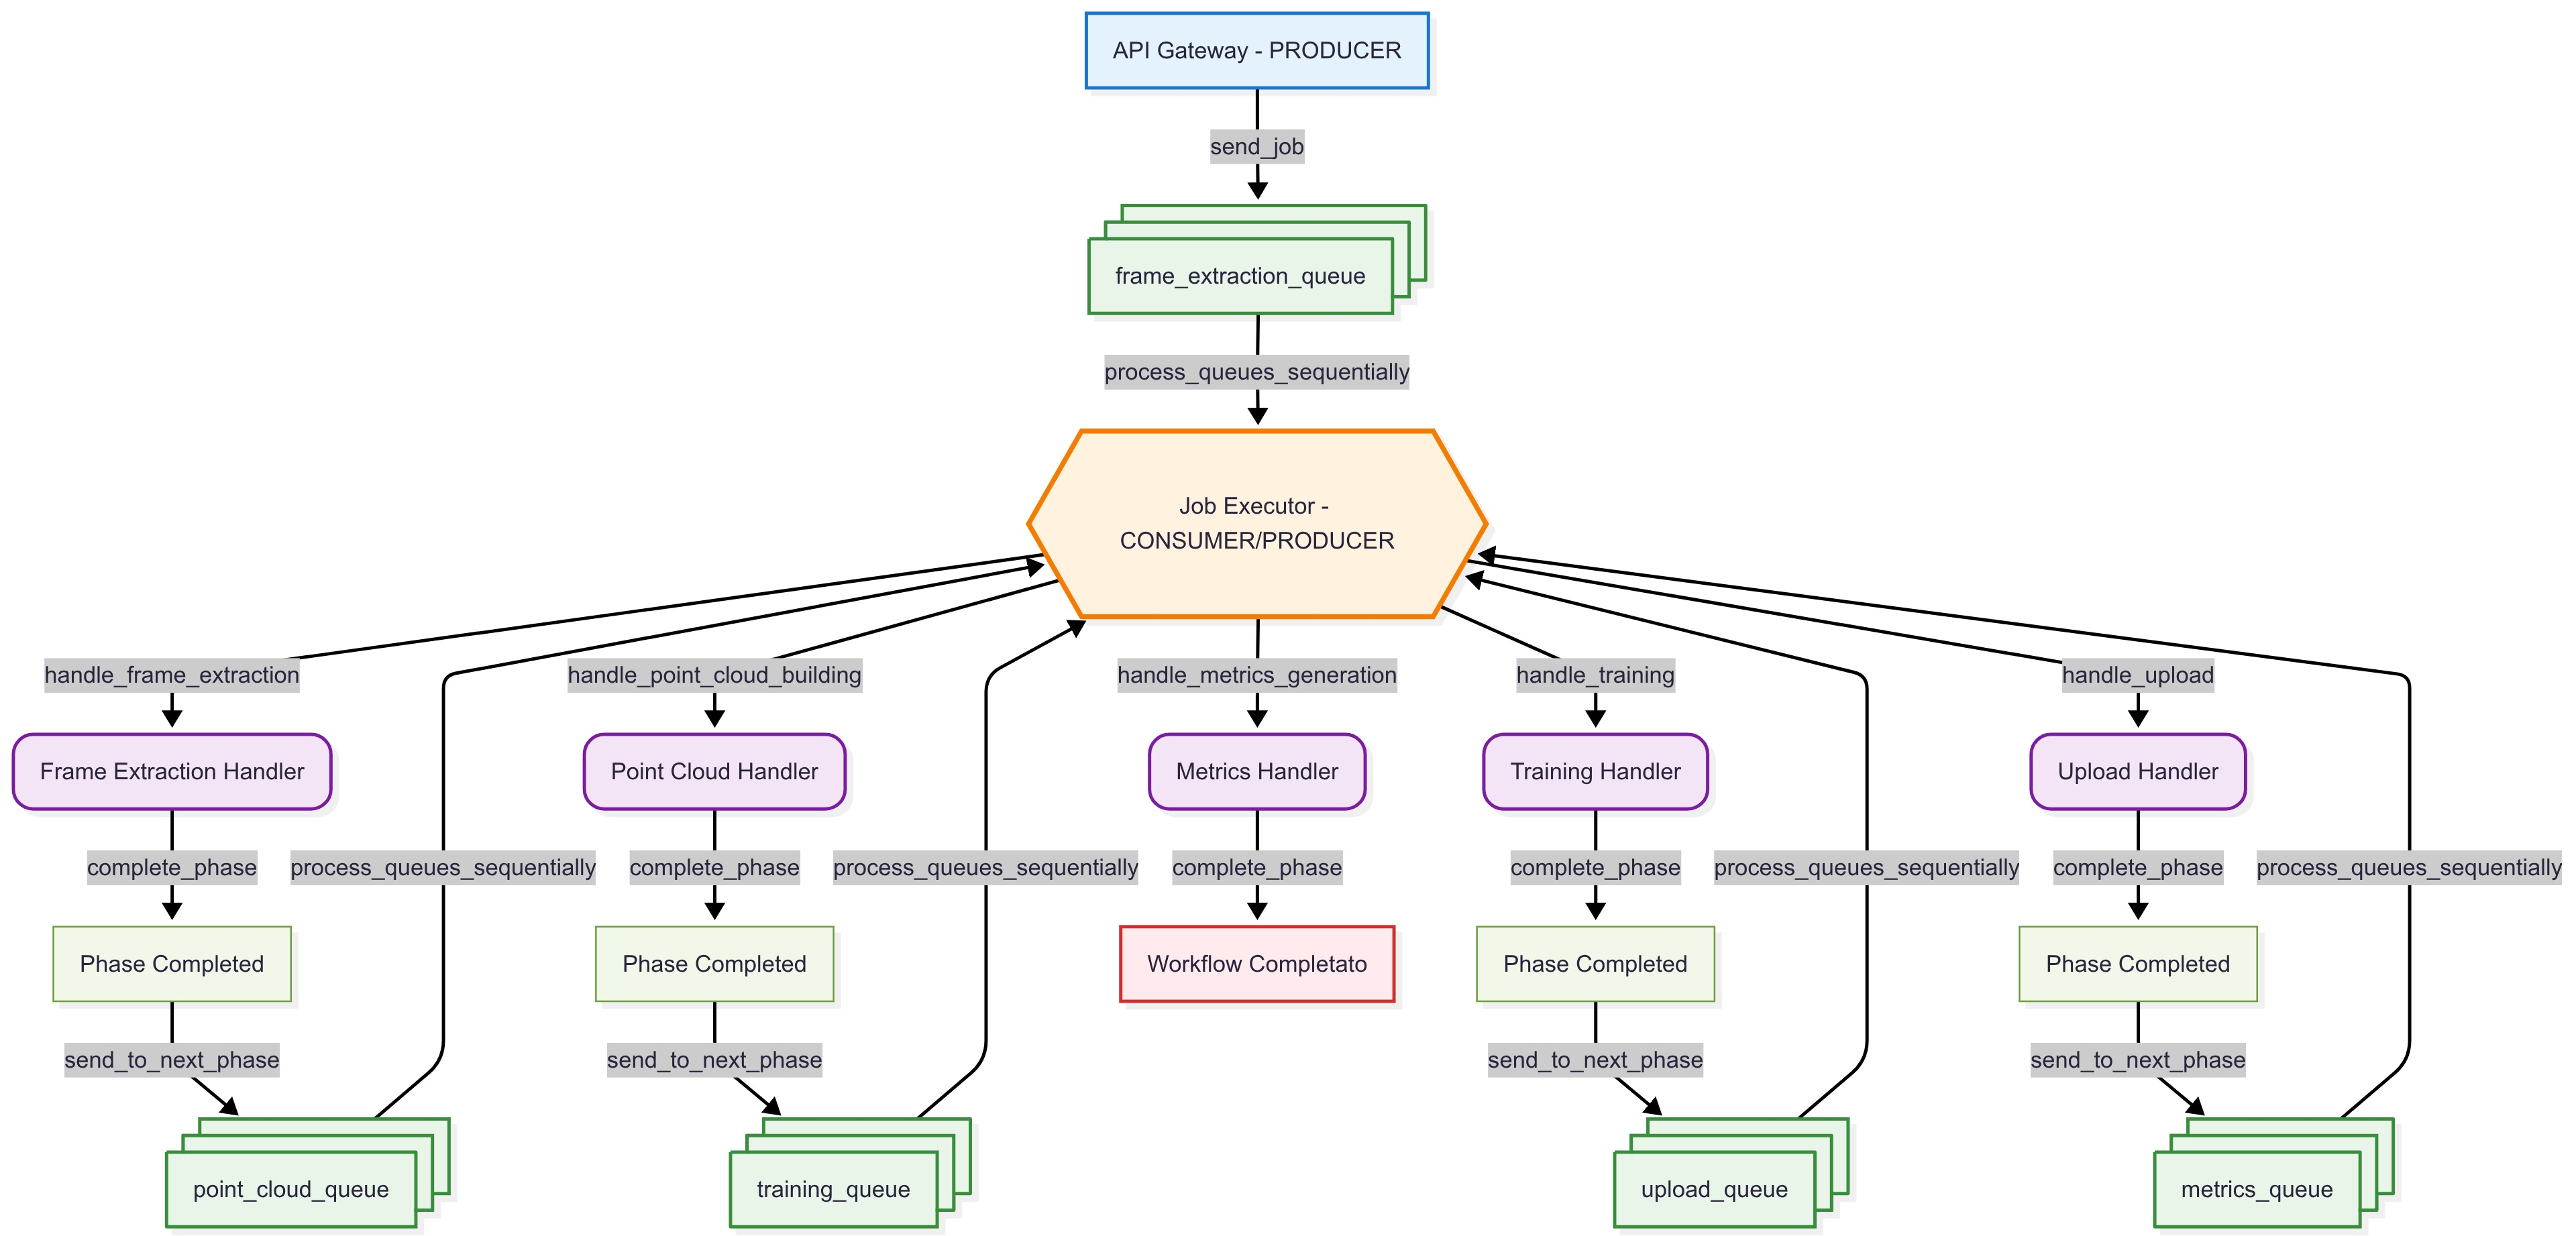
\includegraphics[width=\textwidth]{images/producer_consumer_schema.jpg}
	\caption{Schema del pattern Producer-Consumer ibrido implementato dal Job Executor}
	\label{fig:producer_consumer_schema}
\end{figure}
\newpage
\subsection{Persistenza stati intermedi}

\subsubsection{Pattern di gestione dati intermedi}

Le prime tre fasi del workflow (Frame Extraction, Point Cloud Reconstruction, Training) implementano un pattern specializzato per la gestione dei dati intermedi che abilita funzionalità avanzate di fork e retry.
\newline
Ogni fase salva i propri risultati in archivi compressi standardizzati su Amazon S3, seguendo la convenzione di denominazione \texttt{\{nome\_fase\}\_phase.zip}. Questa struttura permette il recupero selettivo di dati intermedi per operazioni di reprocessing.

\begin{lstlisting}[language=python, caption=Pattern recupero e salvataggio dati intermedi]
	# Recupero dati fase precedente
	success = phase_zip_helper.download_and_extract_phase_zip(
	phase_zip_s3_key, model_dir
	)
	
	# Salvataggio risultati fase corrente
	is_zip_uploaded = phase_zip_helper.create_phase_zip_and_upload(
	model_id, model_dir, PHASE_ZIP_NAME, ['directory_output']
	)
\end{lstlisting}

\subsubsection{Funzionalità di Fork e Retry}
Il pattern dei dati intermedi abilita la \textbf{fork e il retry di modelli} a partire da fasi intermedie, permettendo comparazioni algoritmiche e sperimentazione senza dover ripetere l'intero workflow.

\noindent Ad esempio, un utente potrebbe biforcare un modello completato almeno fino alla fase di Point Cloud Reconstruction per testare un algoritmo di training differente, riutilizzando i la point cloud già generata in precedenza e salvata come dato intermedio su S3. Questo approccio riduce significativamente i tempi di sperimentazione e ottimizza l'utilizzo delle risorse computazionali.

\subsubsection{Gestione fasi secondarie}

Tra le fasi già citate in precedenza, ci sono due fasi che seguono un pattern semplificato per il quale non serve generare dati intermedi persistenti e sono considerate \textbf{secondarie} (seppur fondamentali). Si tratta di:

\begin{itemize}
	\item \textbf{Upload modello finale}: Gestisce la preparazione e il caricamento del modello 3D per la visualizzazione, convertendo i risultati del training in formati ottimizzati per il web viewer.
	
	\item \textbf{Generazione metriche}: Calcola le metriche di qualità (PSNR, SSIM, LPIPS) confrontando rendering di test con immagini ground truth, salvando i risultati direttamente nel database.
\end{itemize}

Separando queste fasi permettiamo la visualizzazione immediata dei modelli 3D generati mentre le metriche vengono calcolate in background: questo migliora l'esperienza utente senza compromettere l'affidabilità del sistema.

\subsection{Resilienza e Fault Tolerance}

Il sistema implementa una strategia di gestione degli errori progettata per garantire continuità operativa attraverso meccanismi di isolamento e persistenza dei dati critici.

\subsubsection{Strategie di Error Handling}

Viene adottato un approccio stratificato per la gestione degli errori, implementando meccanismi di protezione a diversi livelli:

\begin{itemize}
	\item \textbf{Isolamento degli errori}: Il fallimento di un singolo job non compromette l'elaborazione di altri job nel sistema. Ogni workflow opera in modo indipendente, permettendo al sistema di continuare l'elaborazione dei job rimanenti anche in presenza di errori specifici.
	
	\item \textbf{Gestione fallimenti controllata}: Il sistema evita loop infiniti di retry confermando anche i messaggi falliti, delegando la gestione dei retry all'interfaccia utente attraverso funzionalità di restart del modello.
\end{itemize}

\subsubsection{Meccanismi di Persistenza degli Stati}

La resilienza del sistema si basa su diversi meccanismi di persistenza che garantiscono la continuità operativa:

\begin{itemize}
	\item \textbf{Checkpointing degli stati}: Il sistema implementa tracking degli stati di elaborazione attraverso aggiornamenti dei metadati in MongoDB. Il tracking avviene all'inizio e alla fine di ogni fase (\texttt{start\_phase} e \texttt{complete\_phase}), permettendo il monitoraggio del progresso e la gestione dei retry.
	
	\item \textbf{Dati intermedi persistenti}: Le fasi intermedie del workflow vengono salvate come archivi compressi su Amazon S3, abilitando funzionalità di fork e retry senza dover riprocessare l'intero pipeline.
\end{itemize}

\subsubsection{Database Monitoring}

MongoDB fornisce tracking dettagliato dello stato di ogni modello, includendo:

\begin{itemize}
	\item Progressione attraverso le fasi del workflow
	\item Tempi di elaborazione per ogni fase
	\item Metadati completi per troubleshooting e analisi delle performance
	\item Gestione degli stati di errore e recovery
\end{itemize}

Questa architettura di resilienza assicura che il sistema possa operare stabilmente, fornendo meccanismi per il recovery attraverso l'interfaccia utente e mantenendo la visibilità completa sullo stato delle elaborazioni.



\section{Layer di Pre-elaborazione}

Il Layer di Pre-elaborazione rappresenta la fase iniziale critica del workflow, responsabile della trasformazione del contenuto video di input in una rappresentazione geometrica 3D utilizzabile per il training. Questo layer combina due processi sequenziali complementari: l'estrazione intelligente di frame dal video sorgente e la ricostruzione della nuvola di punti 3D attraverso tecniche di Structure from Motion.

\subsection{Architettura del Layer}

Il Layer di Pre-elaborazione è organizzato come pipeline sequenziale che coordina due servizi specializzati:

\begin{enumerate}
	\item \textbf{Video Preprocessing Service}: Trasformazione video in dataset di frame ottimizzato
	\item \textbf{Point Cloud Reconstruction Service}: Ricostruzione geometrica 3D tramite COLMAP
\end{enumerate}

\subsubsection{Strategia di Containerizzazione Differenziata}

Il layer implementa strategie di deployment diverse per i due servizi, basate su considerazioni pragmatiche di complessità e risorse.
\newline
\newline
Il \textbf{Video Preprocessing Service} è mantenuto \textbf{all'interno del container del Job Executor}, a differenza degli altri servizi computazionali che sono containerizzati separatamente.\newpage Questa scelta deriva da valutazioni pragmatiche:

\begin{itemize}
	\item \textbf{Peso computazionale marginale}: Il preprocessing video ha durata contenuta e non impatta l'esecuzione sequenziale dei job
	\item \textbf{Dipendenze leggere}: Utilizzo di librerie esterne facilmente integrabili senza necessità di ambienti dedicati
	\item \textbf{Complessità operativa ridotta}: La separazione introdurrebbe complessità di deploy senza benefici concreti
\end{itemize}

Il \textbf{Point Cloud Reconstruction Service} è implementato come container specializzato basato su PyTorch con supporto CUDA, giustificato da:

\begin{itemize}
	\item \textbf{Complessità computazionale}: Operazioni intensive che richiedono ottimizzazioni specifiche
	\item \textbf{Dipendenze pesanti}: Integrazione di COLMAP e librerie di computer vision specializzate
	\item \textbf{Isolamento computazionale}: Necessità di ambiente dedicato per riproducibilità e gestione risorse
\end{itemize}

\subsection{Video Preprocessing Service}

Il preprocessing video è orchestrato dall'handler \texttt{handle\_frame\_extraction} che funge da punto di connessione tra il sistema di code RabbitMQ e il servizio specializzato. L'handler coordina il flusso di elaborazione delegando le operazioni atomiche al \texttt{VideoFrameExtractionService}, garantendo isolamento delle responsabilità e gestione robusta degli errori.

Il \texttt{VideoFrameExtractionService} implementa tutte le operazioni di preprocessing come servizio atomico, assicurando consistenza e tracciabilità completa del processo attraverso un'unica interfaccia pubblica \texttt{extract\_frames}.

\subsubsection{Pipeline di Preprocessing Video}


\paragraph{1) Download e Validazione}
\mbox{}\\
La pipeline inizia con il recupero del video sorgente dal storage S3 utilizzando il sistema di cache intelligente del \texttt{RepositoryService}, seguito da controlli rigorosi implementati dal metodo \texttt{\_validate\_inputs} per garantire integrità e accessibilità del file video.

\paragraph{2) Analisi Metadati Video}
Il sistema esegue un'analisi completa delle caratteristiche del video attraverso il metodo \texttt{\_analyze\_video}:

\begin{lstlisting}[language=python, caption=Analisi metadati video completa]
	def _analyze_video(self, video_path: str) -> Dict[str, Any]:
	cap = cv2.VideoCapture(video_path)
	original_width = int(cap.get(cv2.CAP_PROP_FRAME_WIDTH))
	original_height = int(cap.get(cv2.CAP_PROP_FRAME_HEIGHT))
	video_fps = cap.get(cv2.CAP_PROP_FPS)
	total_frames = int(cap.get(cv2.CAP_PROP_FRAME_COUNT))
	duration = total_frames / video_fps if video_fps > 0 else 0
	
	# Determinazione orientamento
	is_portrait = original_height > original_width
	
	return {
		'original_width': original_width,
		'original_height': original_height,
		'video_fps': video_fps,
		'duration_seconds': duration,
		'is_portrait': is_portrait,
		'orientation': 'Portrait' if is_portrait else 'Landscape'
	}
\end{lstlisting}

\paragraph{3) Adattamento Orientamento}
Una delle ottimizzazioni più importanti riguarda la gestione intelligente dell'orientamento video:

\begin{lstlisting}[language=python, caption=Logica di adattamento orientamento]
	# Per portrait, target_height diventa la width effettiva
	final_width = target_height if is_portrait else target_width
\end{lstlisting}

I parametri di qualità sono configurati assumendo orientamento landscape standard. Per video portrait, il sistema utilizza \texttt{target\_height} come dimensione principale per mantenere la qualità visiva desiderata.

\paragraph{4) Calibrazione FPS per Target Frame}
Il cuore del preprocessing è la calibrazione intelligente del frame rate di estrazione:

\begin{lstlisting}[language=python, caption=Algoritmo di calibrazione FPS]
	if duration > 0:
		extraction_fps = target_frame_count / duration
		extraction_fps = min(extraction_fps, video_fps)  # Vincolo hardware
		extraction_fps = max(0.5, extraction_fps)        # Soglia qualità minima
	else:
		extraction_fps = 1.0  # Fallback sicuro
\end{lstlisting}

Sebbene il numero di frame target sia teoricamente parametrizzabile attraverso il sistema di parametrizzazione adattiva, la configurazione attuale fissa questo valore a 200 frame, identificato come ottimale per bilanciare qualità della ricostruzione e efficienza computazionale.

\paragraph{5) Estrazione Frame con Sharp-Frames}
L'estrazione utilizza il tool specializzato Sharp-Frames con configurazione ottimizzata per la pipeline COLMAP:

\begin{lstlisting}[language=python, caption=Configurazione Sharp-Frames ottimizzata]
	cmd = [
	"sharp-frames",
	video_path,
	output_directory,
	"--selection-method", "best-n",
	"--min-buffer", "1",
	"--fps", str(optimized_params['extraction_fps'])
	]
	
	# Aggiunta parametro width se necessario
	final_width = optimized_params.get('final_width')
	if final_width is not None:
	cmd.extend(["--width", str(final_width)])
\end{lstlisting}

La scelta del metodo \texttt{best-n} prioritizza la qualità dei singoli frame, aspetto critico per il successo delle fasi successive di feature matching in COLMAP.

\paragraph{6) Finalizzazione e Persistenza}
Il processo conclude con validazione output, generazione thumbnail per il layer di presentazione, creazione archivio fase per supportare fork/retry, e generazione metadati dettagliati per tracciabilità completa.

\begin{figure}[htbp]
	\centering
	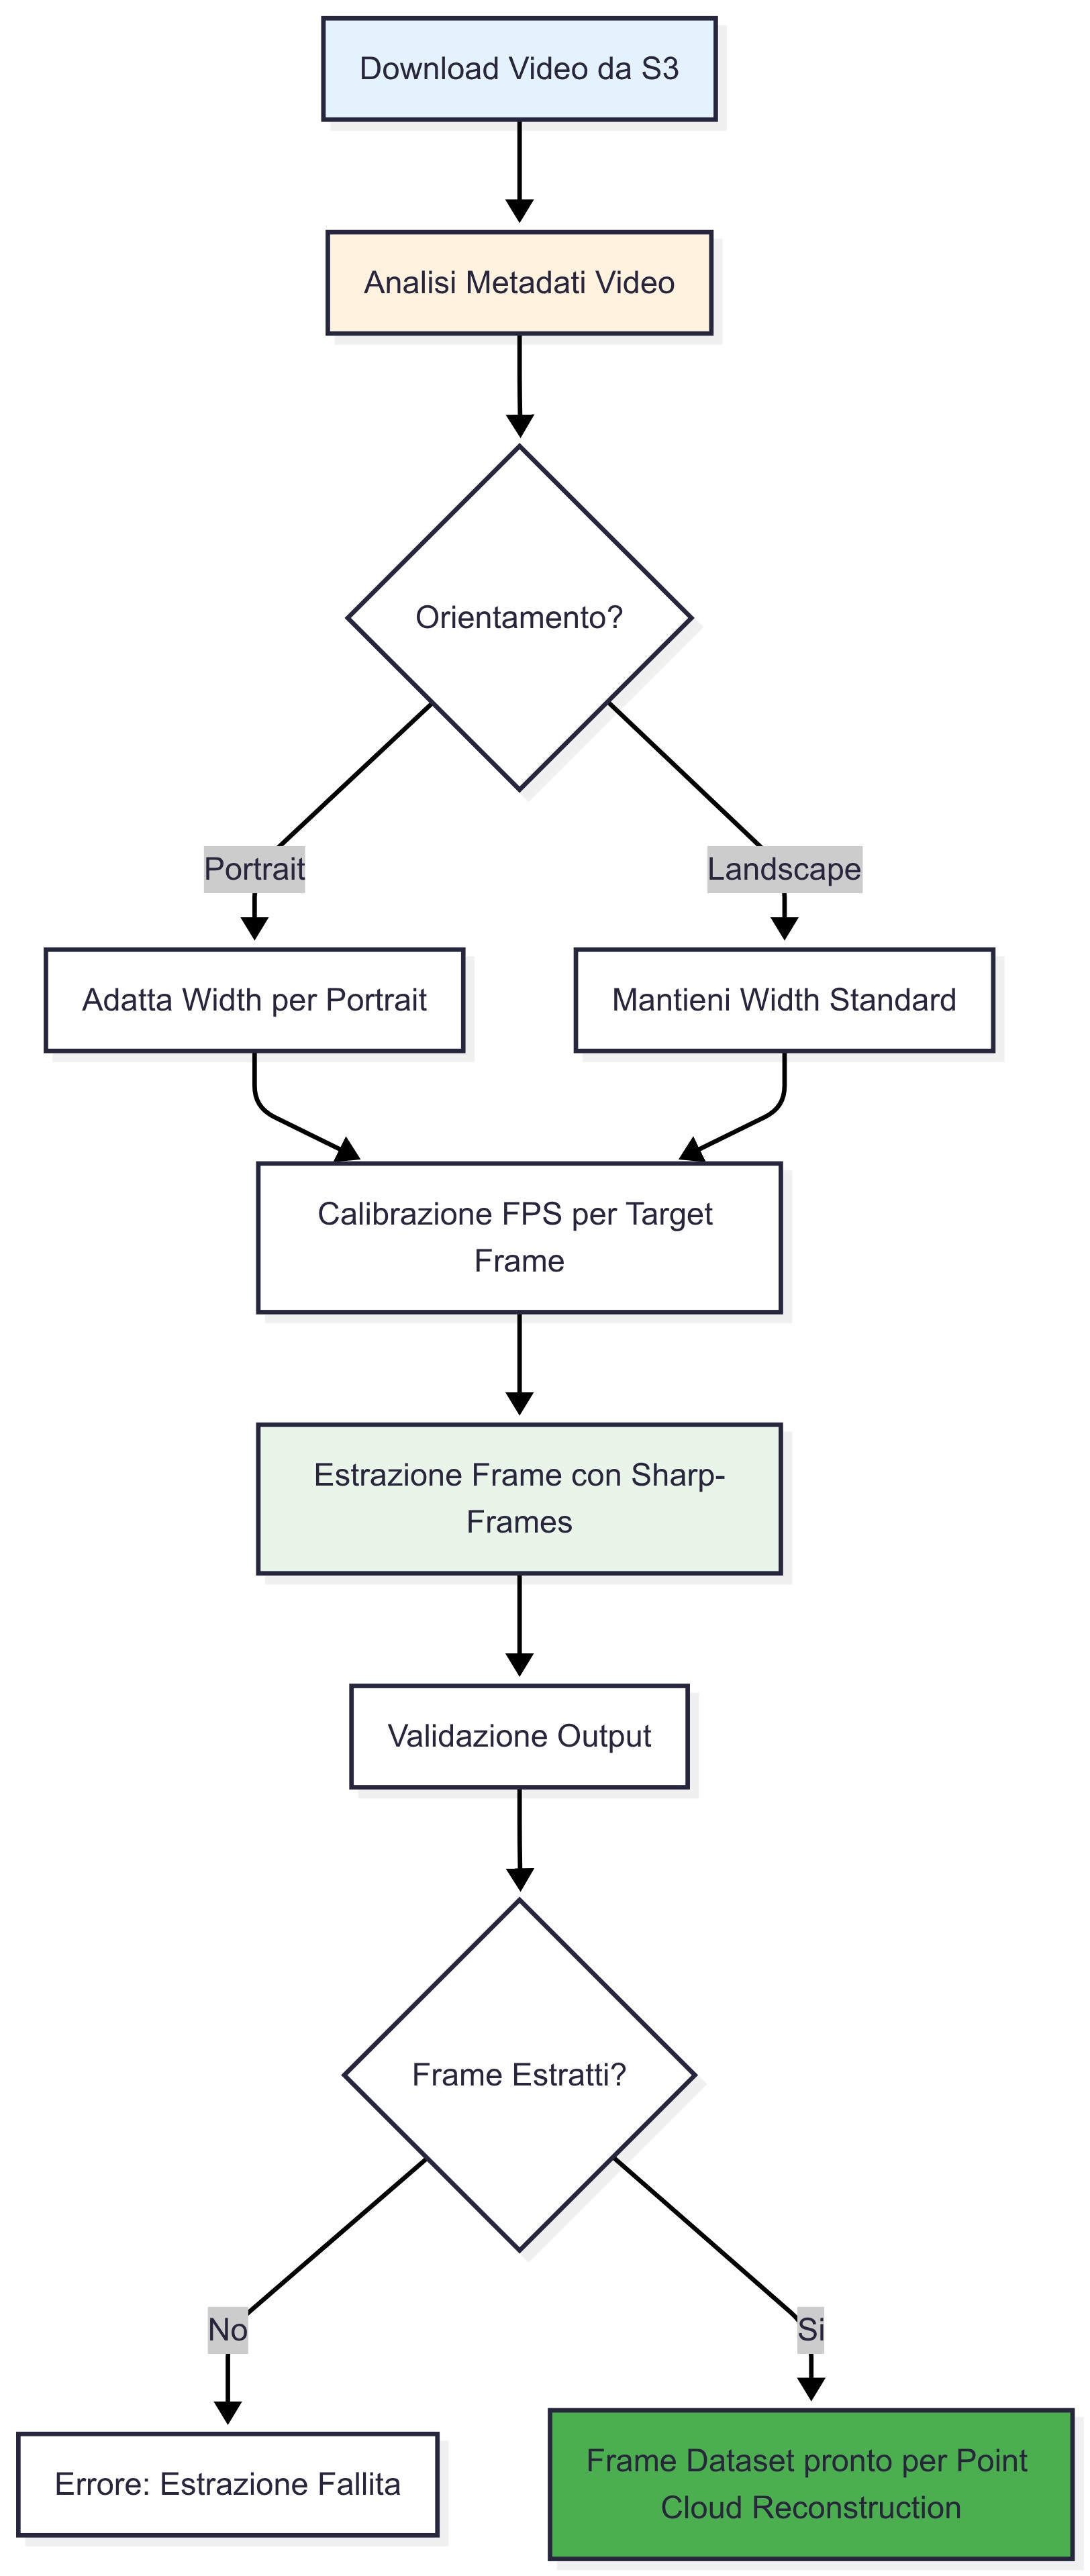
\includegraphics[width=0.6\textwidth]{images/frame_extraction_diagram.jpg}
	\caption{Schema del estrazione frames da video}
	\label{fig:frame_extraction_diagram}
\end{figure}
\newpage
\subsection{Point Cloud Reconstruction Service}

\subsubsection{Handler Point Cloud Building}
La Point Cloud Reconstruction è orchestrata dall'handler \texttt{handle\_point\_cloud\_building} che coordina la ricostruzione della nuvola di punti 3D a partire dal dataset di frame ottimizzato.

\paragraph{Recupero Dataset e Validazione}
Il sistema recupera il dataset di frame dalla fase precedente, gestendo automaticamente diverse fonti tramite il pattern di dati intermedi.

\paragraph{Generazione Point Cloud via COLMAP}
La ricostruzione avviene tramite chiamata al servizio COLMAP containerizzato con analisi automatica della strategia ottimale:

\begin{lstlisting}[language=python, caption=Generazione point cloud con monitoraggio performance]
	sparse_dir = os.path.join(model_dir, 'sparse')
	
	colmap_start_time = datetime.utcnow()
	
	# COLMAP API call con analisi automatica strategia
	convert_request = {"input_dir": model_dir}
	response = requests.post(COLMAP_API_URL + "/convert", json=convert_request)
	
	colmap_duration_seconds = (datetime.utcnow() - colmap_start_time).total_seconds()
	
	# Verifica output e raccolta statistiche
	generated_points = job_utils.get_colmap_reconstruction_stats(model_dir)
\end{lstlisting}

\subsubsection{Strategie di Feature Matching: Analisi Comparativa}

\begin{itemize}
\item \textbf{Exhaustive Matching}: la strategia exhaustive confronta ogni immagine con tutte le altre nel dataset, con \textbf{complessità O(n²)}. Garantisce qualità massima per dataset fino a diverse centinaia di immagini, ha tempi di elaborazione che variano da 2 a 5 minuti per scene rappresentate da circa 200 immagini a seconda della loro complessità.

\item \textbf{Sequential Matching}:
la strategia sequential sfrutta l'ordine temporale dei frame video, con \textbf{complessità O(n × overlap)}. Offre efficienza temporale significativa ma produce point cloud meno dense che richiedono maggiore sforzo durante le fasi di pruning e densification del training Gaussian Splatting.

\item \textbf{Vocabulary Tree Matching}:
la strategia vocabulary tree utilizza un albero di vocabolario precompilato, con \textbf{complessità O(n log n)}. È ottimale per grandi dataset (migliaia di immagini) e offre una qualità molto vicina a quella dela strategia exhaustive quando la quantità di feature media è bassa.
\end{itemize}	
\subsubsection{Pipeline di Ricostruzione Ottimizzata}

Il processo include feature extraction parametrizzata, bundle adjustment ottimizzato con tolleranze specifiche, e generazione di statistiche dettagliate per tracciabilità e debugging.

\subsection{Integrazione e Coordinamento}

\subsubsection{Flusso di Dati tra Servizi}

Il layer implementa un flusso di dati efficiente attraverso il pattern di archivi intermedi:

\begin{enumerate}
	\item \textbf{Video Preprocessing}: Genera archivio \texttt{point\_cloud\_building\_phase.zip} contenente frame estratti
	\item \textbf{Point Cloud Reconstruction}: Consuma frame e genera archivio \texttt{training\_phase.zip} con nuvola di punti
	\item \textbf{Handoff al Training}: Fornisce dataset completo per gli algoritmi Gaussian Splatting
\end{enumerate}

\subsubsection{Gestione Metadati e Performance}

Entrambi i servizi generano metadati dettagliati che documentano:

\begin{itemize}
	\item \textbf{Parametri di elaborazione}: Configurazioni utilizzate per riproducibilità
	\item \textbf{Statistiche quantitative}: Conteggi frame, punti 3D generati, tempi di elaborazione
	\item \textbf{Performance data}: Metriche per analisi e ottimizzazioni future
	\item \textbf{Versioning}: Tracciabilità delle versioni software utilizzate
\end{itemize}

Il Layer di Pre-elaborazione rappresenta quindi un componente critico e sofisticato che, attraverso l'integrazione intelligente di algoritmi di preprocessing video e ricostruzione geometrica 3D, trasforma contenuti video grezzi in rappresentazioni geometriche ottimizzate per il training Gaussian Splatting, garantendo qualità, efficienza e tracciabilità completa del processo.

\section{Layer di Training}

Il motore di training rappresenta il cuore computazionale del sistema, responsabile dell'esecuzione degli algoritmi di Gaussian Splatting. L'implementazione adotta un approccio containerizzato che isola ogni algoritmo in un ambiente dedicato, esponendo le funzionalità attraverso API REST standardizzate.

\subsection{Architettura containerizzata multi-algoritmo}

Il sistema implementa tre container specializzati, ciascuno dedicato a un algoritmo specifico:

\begin{itemize}
	\item \textbf{gaussian-splatting}: Implementazione di riferimento del paper originale
	\item \textbf{3dgs-mcmc}: Variante con campionamento MCMC per ottimizzazione stocastica  
	\item \textbf{taming-3dgs}: Versione ottimizzata per scene complesse
\end{itemize}

Ogni container segue una strategia di build multi-stage per ottimizzare le dimensioni e i tempi di compilazione:

\subsection{Handler Training}

L'handler di training coordina l'esecuzione degli algoritmi di Gaussian Splatting, gestendo la configurazione dei parametri e le funzionalità specifiche come la depth regularization per il motore standard.

\subsubsection{Recupero Dataset e Configurazione}

Il sistema recupera la point cloud e le immagini processate dalla fase precedente, configurando dinamicamente i parametri in base all'algoritmo selezionato:

\begin{lstlisting}[language=python, caption=Inizializzazione e configurazione training]
	model_service.start_phase(model_id, "training")
	model = model_service.get_model_by_id(model_id)
	
	model_dir = os.path.join(WORKING_DIR, f"{model_id}")
	image_dir = os.path.join(model_dir, "images")
	sparse_dir = os.path.join(model_dir, "sparse")
	
	# Recupera ZIP dalla fase point cloud building se necessario
	if not (os.path.exists(image_dir) and os.path.exists(sparse_dir)):
	training_zip_s3_key = f"{S3_STAGING_PREFIX}/{model.parent_model_id}/{TRAINING_PHASE_ZIP_NAME}"
	success = phase_zip_helper.download_and_extract_phase_zip(
	training_zip_s3_key, model_dir
	)
	
	# Configurazione parametri tramite TrainingParamsService
	engine = model.training_config.get('engine')
	quality_level = model.training_config.get('quality_level')
	
	generated_params = training_params_service.generate_params(
	Engine(engine), QualityLevel(quality_level)
	)
\end{lstlisting}

\subsubsection{Depth Regularization per Gaussian Splatting standard}

Per il motore \textit{Gaussian Splatting} standard, viene implementata una fase di \textbf{depth regularization}, come suggerito dalla documentazione ufficiale, al fine di migliorare la qualità della ricostruzione nelle scene real-world.
Questa tecnica vincola le gaussiane a disporsi lungo superfici coerenti con le stime di profondità ottenute dalle immagini, riducendo la presenza di artefatti e gaussiane fluttuanti nello spazio 3D, tipiche delle scene acquisite dal mondo reale.

Nel caso delle varianti \textbf{MCMC} e \textbf{Taming}, invece, non viene impiegata depth regularization esplicita.
Queste versioni adottano strategie di ottimizzazione alternative — rispettivamente, tramite sampling stocastico e controlli specifici sulla crescita e la fusione delle gaussiane — che mitigano la formazione di outlier e favoriscono la distribuzione regolare delle gaussiane nello spazio, rendendo la regularizzazione sulla profondità meno necessaria.

È importante sottolineare che la presenza della depth regularization, pur migliorando la plausibilità geometrica della scena, \textbf{può in alcuni casi limitare le performance su metriche quantitative come il PSNR}, poiché impone vincoli aggiuntivi rispetto all’ottimizzazione puramente basata sulla ricostruzione delle immagini.

\begin{lstlisting}[language=python, caption=Endpoint depth regularization]
	@app.post("/depth_regularization")
	async def make_depth_regularization(request: DepthRegularizationRequest):
	logger.info(f"Starting depth generation - Input directory: {request.input_dir}")
	
	images_dir = os.path.join(request.input_dir, 'images')
	depths_dir = os.path.join(request.input_dir, 'depths')
	
	# STEP 1: Genera depth maps con Depth Anything V2
	depth_command = (
	f"cd /workspace/Depth-Anything-V2 && "
	f"python3 run.py --encoder vitl --pred-only --grayscale "
	f"--img-path {images_dir} --outdir {depths_dir}"
	)
	
	# Esecuzione depth generation con logging multi-thread
	depth_process = subprocess.Popen(
	depth_command, shell=True, stdout=subprocess.PIPE, 
	stderr=subprocess.PIPE, text=True, bufsize=1
	)
	
	# [Thread management per logging real-time]
	
	# STEP 2: Genera depth_params.json con scaling automatico
	params_command = (
	f"python3 /workspace/gaussian-splatting/utils/make_depth_scale.py "
	f"--base_dir {request.input_dir} --depths_dir {depths_dir}"
	)
	
	# [Esecuzione simile con thread management]
	
	return {
		"message": "Depth generation and params completed successfully",
		"depth_maps_count": depth_count,
		"depth_maps_dir": depths_dir
	}
\end{lstlisting}

\subsubsection{Esecuzione Training}

Il sistema seleziona dinamicamente l'API dell'engine containerizzato corrispondente e avvia il processo di training:

\begin{lstlisting}[language=python, caption=Esecuzione training con engine selezionato]
	# Selezione API engine dalla mappatura
	api_url = engine_map.get(engine, {}).get('api-url')
	if not api_url:
	self.fail(model_id, "training", f"Error: No api url found for engine {engine}")
	return False
	
	# Costruzione richiesta di training
	train_request = {
		"input_dir": model_dir,
		"output_dir": train_output_folder,
		"params": generated_params.final_params,  # Parametri ottimizzati
	}
	
	print(f"🎯 Starting training with engine: {engine}")
	training_start_time = datetime.utcnow()
	
	# Chiamata API training containerizzato
	response = requests.post(f"{api_url}/train", json=train_request)
	
	training_end_time = datetime.utcnow()
	training_duration = training_end_time - training_start_time
	training_duration_seconds = training_duration.total_seconds()
	
	if response.status_code != 200:
	self.fail(model_id, "training", f"Training failed: {response.text}")
	return False
\end{lstlisting}

\subsubsection{Finalizzazione e Metadati}

La fase si conclude con l'aggiornamento dei metadati, includendo statistiche di performance e informazioni sulla depth regularization:

\begin{lstlisting}[language=python, caption=Finalizzazione training con metadati estesi]
	# Aggiorna metadati con statistiche complete
	phase_metadata = {
		"training_duration_seconds": round(training_duration_seconds, 2),
		"depth_regularization_seconds": round(depth_duration_seconds, 2),
		"training_start_time": training_start_time.isoformat(),
		"training_end_time": training_end_time.isoformat(),
		"training_parameters": {
			"engine": engine,
			"quality_level": quality_level,
			"final_params": generated_params.final_params,
			"depth_regularization_enabled": engine == Engine.INRIA.value
		}
	}
	
	model_service.complete_phase(model_id, "training", metadata=phase_metadata)
\end{lstlisting}

\subsection{Interfaccia API REST unificata}

\subsubsection{Standardizzazione degli endpoint}

Ogni container espone un'interfaccia REST standardizzata che astrae le specificità implementative degli algoritmi sottostanti:

\begin{lstlisting}[language=python, caption=Definizione modelli dati per API REST]
	from fastapi import FastAPI, HTTPException
	from pydantic import BaseModel, Field
	import subprocess
	import threading
	import queue
	import logging
	from typing import Dict, Any
	
	app = FastAPI()
	
	class TrainRequest(BaseModel):
	input_dir: str  
	output_dir: str
	params: Dict[str, Any] = Field(
	default_factory=dict, 
	description="Parametri specifici dell'algoritmo"
	)
	
	class RenderRequest(BaseModel):
	output_dir: str  
	
	class MetricsRequest(BaseModel):
	output_dir: str
	
	class DepthRegularizationRequest(BaseModel):
	input_dir: str
\end{lstlisting}

\subsubsection{Gestione parametri dinamica}

La gestione dei parametri di training è implementata attraverso un sistema dinamico che costruisce automaticamente gli argomenti della command line:

\begin{lstlisting}[language=python, caption=Costruzione dinamica comando di training]
	@app.post("/train")
	async def run_train(request: TrainRequest):
	logger.info(f"Starting training - Input: {request.input_dir}")
	
	# Costruzione dinamica del comando
	command = ["python3", "/workspace/gaussian-splatting/train.py"]
	depths_dir = os.path.join(request.input_dir, 'depths')
	
	# Parametri obbligatori con depth regularization
	command.extend([
	"--resolution", "1",
	"-s", request.input_dir,
	"-m", request.output_dir,
	"-d", depths_dir  # Directory depth maps per regularization
	])
	
	# Parametri dinamici dall'utente
	boolean_flags = {"eval"}
	
	for param_key, value in request.params.items():
		if param_key in boolean_flags:
			if value:
				command.append(f"--{param_key}")
			elif param_key != 'resolution':
				command.extend([f"--{param_key}", str(value)])
	
	# Flag antialiasing automatico
	command.append(f"--antialiasing")
	
	# Esecuzione con logging real-time multi-thread
	# [Implementazione gestione processo e thread]
\end{lstlisting}

\subsubsection{Endpoint Specializzati}

Oltre al training principale, ogni container espone endpoint per le fasi complementari del workflow:

\begin{itemize}
	\item \textbf{\texttt{/train}}: Esecuzione dell'algoritmo di training principale
	\item \textbf{\texttt{/render}}: Generazione delle immagini di test per validazione
	\item \textbf{\texttt{/metrics}}: Calcolo delle metriche di qualità (PSNR, SSIM, LPIPS)
	\item \textbf{\texttt{/depth\_regularization}}: Generazione depth maps (solo gaussian-splatting standard)
\end{itemize}

\subsection{Handler Metrics Generation}
L'handler di metrics generation rappresenta la fase finale del workflow, responsabile della valutazione quantitativa del modello addestrato attraverso metriche standard di qualità visiva. Come per l'upload, questa fase è stata isolata strategicamente per permettere al modello di essere disponibile per il rendering mentre le metriche vengono calcolate in background.
\subsubsection{Inizializzazione e Validazione Output}
Il sistema verifica la disponibilità dell'output di training e prepara l'ambiente per la generazione delle metriche di valutazione:
\begin{lstlisting}[language=python, caption=Inizializzazione e validazione output training]
	model_service.start_phase(model_id, "metrics_evaluation")
	model = model_service.get_model_by_id(model_id)
	model_dir = os.path.join(WORKING_DIR, f"{model_id}")
	Verifica esistenza output del training
	output_dir = os.path.join(model_dir, 'output')
	if not os.path.exists(output_dir):
	self.fail(model_id, "metrics_evaluation", f"No folder output found")
	return False
	engine = model.training_config.get('engine', 'INRIA')
\end{lstlisting}
\subsubsection{Generazione render e calcolo metriche}
Il sistema utilizza lo stesso engine containerizzato del training per generare render di valutazione e calcolare le metriche standard di qualità visiva (SSIM, PSNR, LPIPS):
\begin{lstlisting}[language=python, caption=Generazione render e calcolo metriche]
	engine = model.training_config.get('engine', 'INRIA')
	Generazione render per valutazione
	render_request = {"output_dir": output_dir}
	response = requests.post(engine_map.get(engine).get('api-url') + "/render", json=render_request)
	response.raise_for_status()
	Calcolo metriche di qualità
	metrics_request = {"output_dir": output_dir}
	response = requests.post(engine_map.get(engine).get('api-url') + "/metrics", json=metrics_request)
	response.raise_for_status()
	Verifica generazione del file risultati
	results_json_path = os.path.join(output_dir, "results.json")
	if not os.path.exists(results_json_path):
	raise FileNotFoundError("Il file 'results.json' non è stato trovato.")
	with open(results_json_path, 'r') as f:
	results_data = json.load(f)
\end{lstlisting}
\newpage
\subsubsection{Finalizzazione e Persistenza Metriche}
La fase si conclude con la persistenza delle metriche calcolate nei metadati del modello, rendendo immediatamente disponibili per visualizzazione nel frontend:
\begin{lstlisting}[language=python, caption=Persistenza metriche e completamento workflow]
	Salvataggio metriche nei metadati del modello
	model_service.complete_phase(
	model_id,
	"metrics_evaluation",
	overall_status="COMPLETED",
	metadata={"metrics": results}
	)
	print(f"✅ Metriche generate e salvate per model {model_id}")
\end{lstlisting}

La gestione intelligente delle chiavi del file JSON è fondamentale perché il nome delle sezioni include il numero di iterazioni specificato nella parametrizzazione (es. \texttt{ours\_30000} per 30.000 iterazioni). Questo collegamento diretto tra parametri di training e struttura delle metriche garantisce che la valutazione sia sempre coerente con la configurazione utilizzata per l'addestramento. L'isolamento di questa fase permette all'utente di visualizzare il modello 3D immediatamente dopo l'upload, mentre le metriche vengono calcolate in background e aggiornate progressivamente nell'interfaccia.

\section{Layer Backend-for-Frontend}

\subsection{Architettura e Funzionalità Principali}

Il layer Backend-for-Frontend (API Gateway) funge da punto di accesso unico e sicuro per tutte le operazioni sui modelli 3D, orchestrando la comunicazione tra frontend, database MongoDB, sistema di code RabbitMQ e storage S3 (Fig. \ref{fig:bff_architecture}).

\begin{figure}[H]
	\centering
	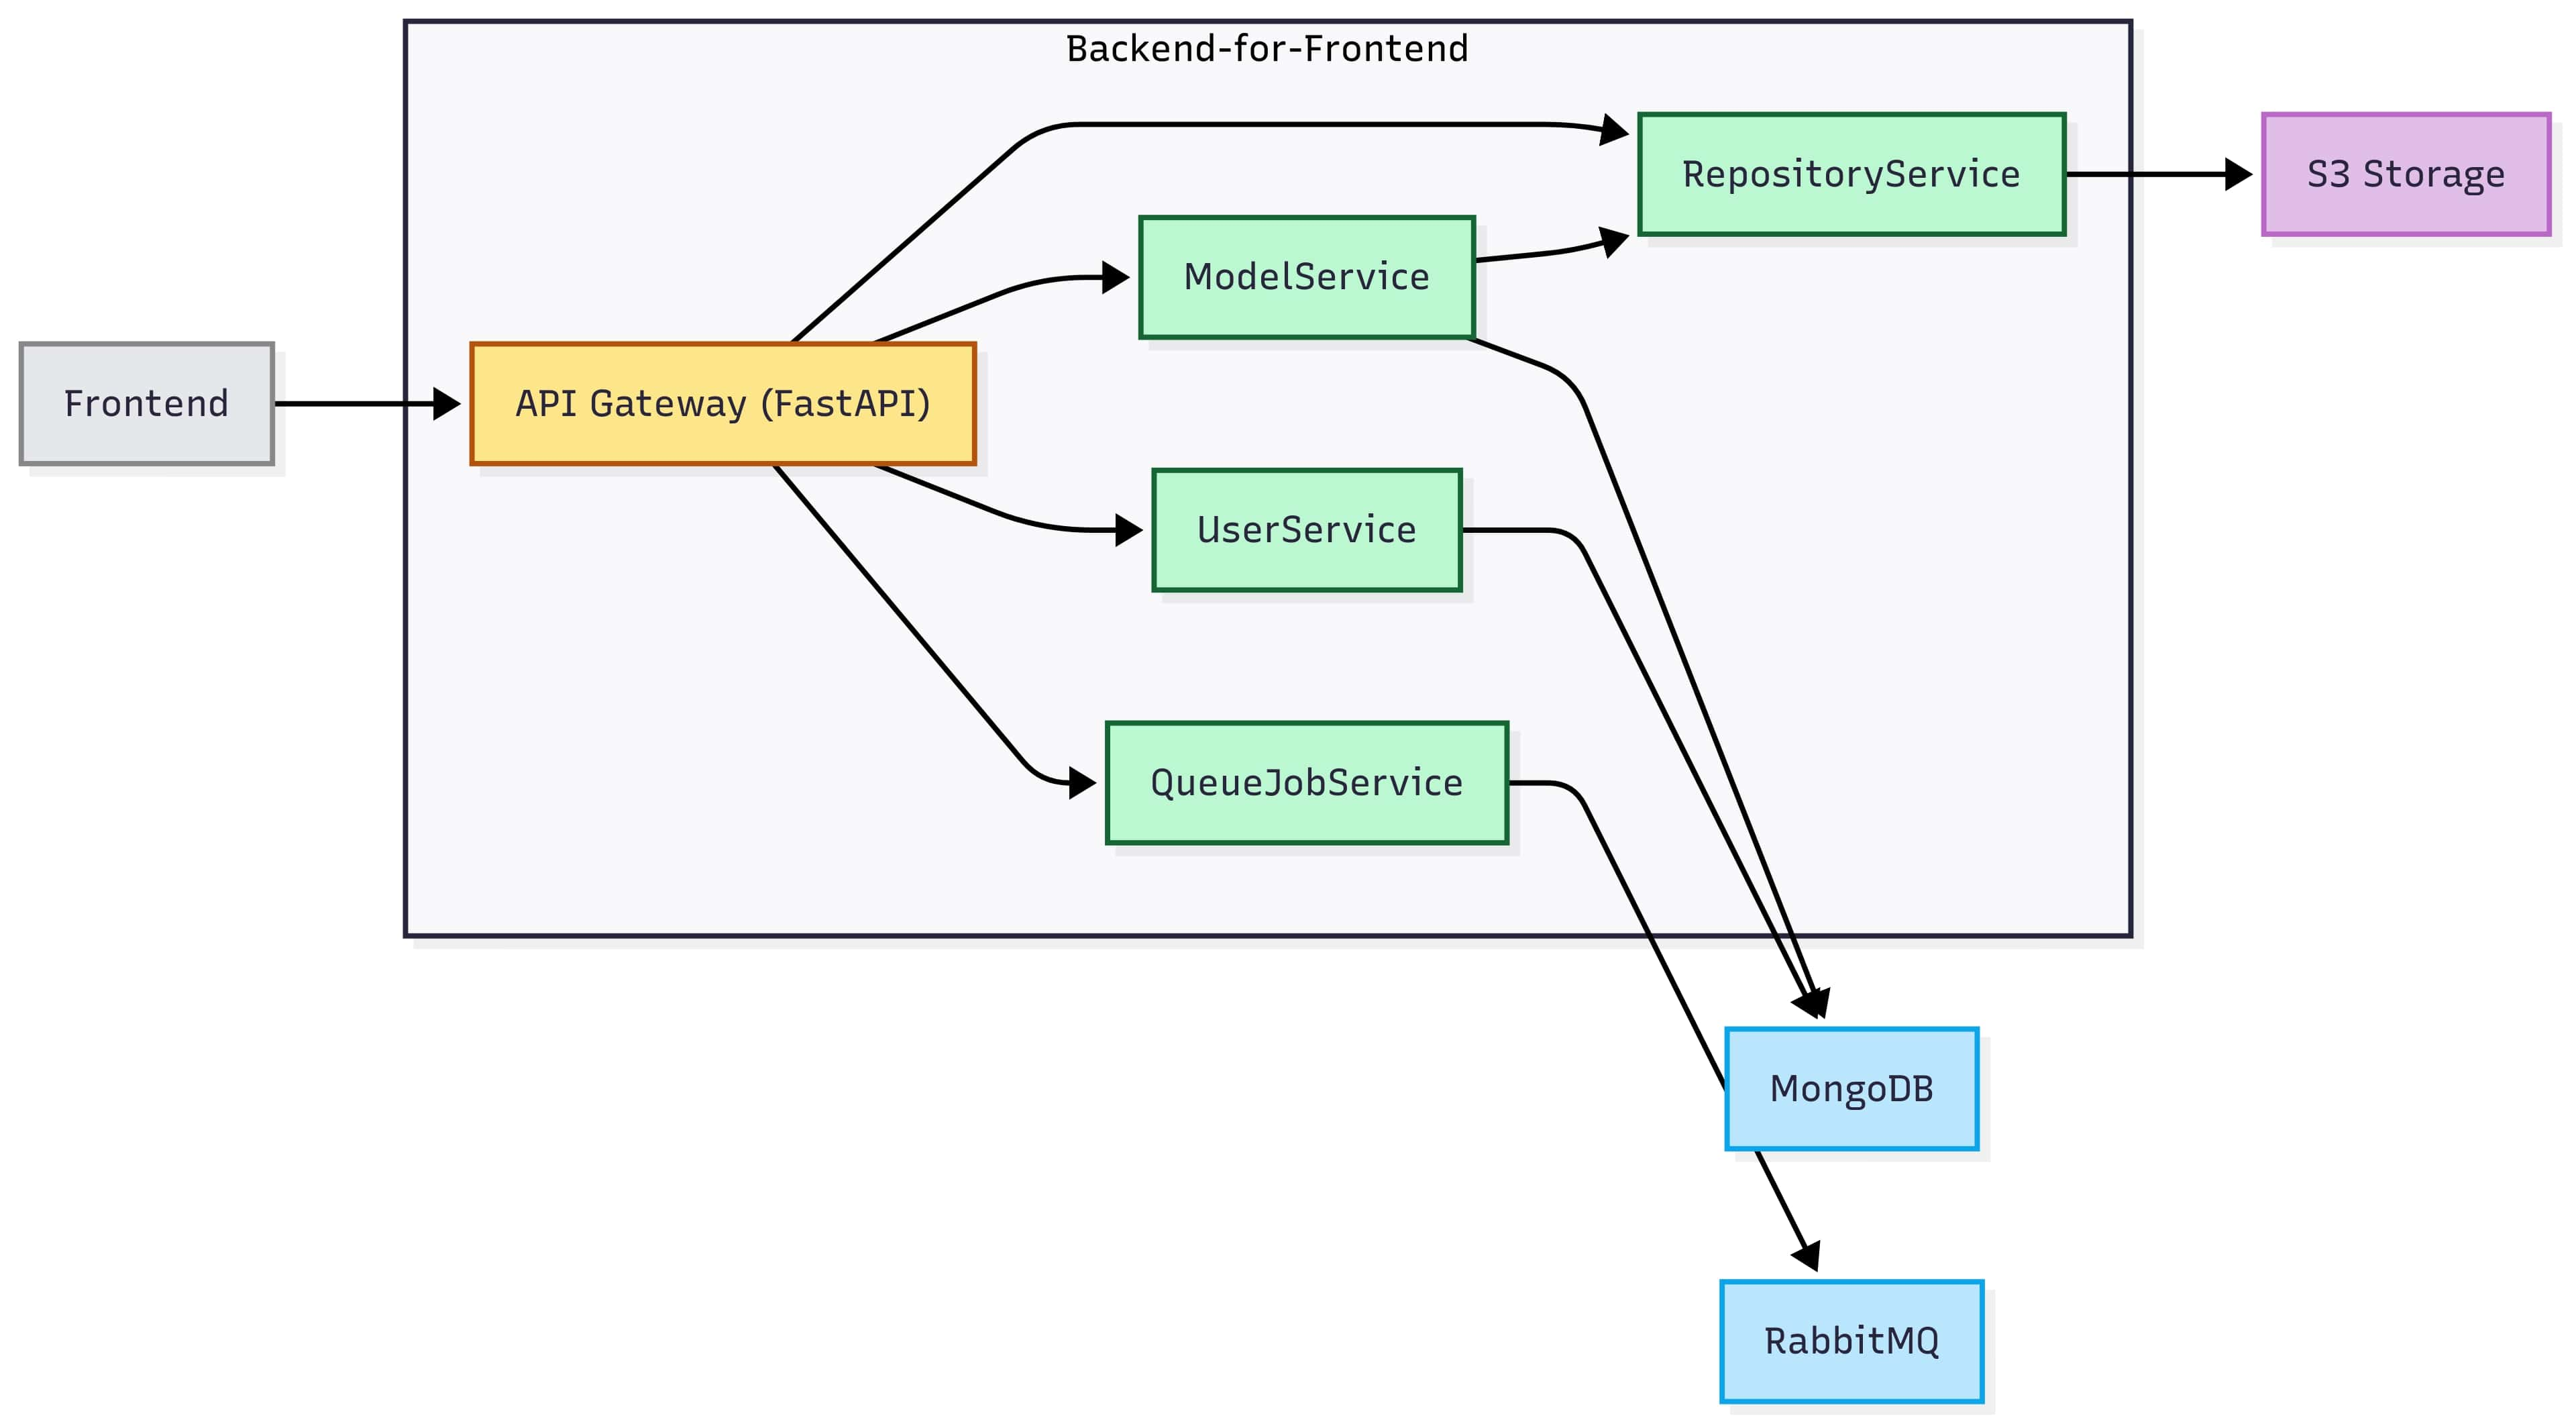
\includegraphics[width=0.9\textwidth]{images/bff_architecture.jpg}
	\caption{Architettura del layer Backend-for-Frontend}
	\label{fig:bff_architecture}
\end{figure}

\subsection{Riepilogo Endpoint REST e WebSocket}

La Tabella~\ref{tab:endpoint_bff} riepiloga i principali endpoint esposti dall'API Gateway.

\begin{table}[H]
	\centering
	\begin{tabular}{|l|l|l|l|}
		\hline
		Metodo & Endpoint & Descrizione & Autenticazione \\
		\hline
		POST & /register & Registrazione utente admin & Basic Auth \\
		POST & /token & Login e rilascio JWT & Nessuna \\
		POST & /models/ & Creazione nuovo modello & Basic Auth \\
		GET & /models/ & Elenco modelli & Basic Auth \\
		GET & /models/\{id\} & Dettaglio modello & Basic Auth \\
		POST & /models/\{id\}/retry & Retry modello fallito & Basic Auth \\
		DELETE & /models/\{id\} & Eliminazione modello & Basic Auth \\
		POST & /s3/upload-url/ & Generazione presigned URL S3 & Basic Auth \\
		GET & /health & Health check API & Nessuna \\
		WS & /ws/notifications & Notifiche real-time & -- \\
		\hline
	\end{tabular}
	\caption{Principali endpoint esposti dall’API Gateway}
	\label{tab:endpoint_bff}
\end{table}

\subsection{Logica e Flussi Principali degli Endpoint}

\subsubsection{Registrazione e Autenticazione}

\begin{itemize}
	\item \textbf{Registrazione} (\texttt{POST /register}): Consente la creazione di nuovi utenti admin, protetta tramite HTTP Basic Authentication.
	\item \textbf{Login} (\texttt{POST /token}): Permette agli utenti di autenticarsi tramite username e password e ricevere un JWT per l’accesso alle altre API.
\end{itemize}

\subsubsection{Gestione Modelli 3D}

\begin{itemize}
	\item \textbf{Creazione modello} (\texttt{POST /models/}): Permette la creazione di un nuovo modello 3D (ex novo o fork). Il servizio:
	\begin{enumerate}
		\item Valida la richiesta e crea il modello su MongoDB.
		\item Invia un job di elaborazione su RabbitMQ.
		\item Restituisce le informazioni del nuovo modello.
	\end{enumerate}
	\item \textbf{Elenco modelli} (\texttt{GET /models/}): Restituisce una lista di modelli 3D con supporto a paginazione, filtri (per nome e stato) e ordinamento.
	\item \textbf{Dettaglio modello} (\texttt{GET /models/\{id\}}): Recupera tutti i dettagli di un modello tramite il suo identificatore unico.
	\item \textbf{Retry modello} (\texttt{POST /models/\{id\}/retry}): Permette di riavviare l’elaborazione di un modello che ha subito un errore in una delle fasi.
	\item \textbf{Eliminazione modello} (\texttt{DELETE /models/\{id\}}): Consente di rimuovere un modello dal database (implementazione futura).
\end{itemize}

\subsubsection{Gestione Upload Video}

\begin{itemize}
	\item \textbf{Generazione presigned URL} (\texttt{POST /s3/upload-url/}): Genera un URL presigned che consente l’upload sicuro di file video direttamente su S3, riducendo il carico sull’API Gateway.
\end{itemize}

\subsubsection{Notifiche Real-time}

\begin{itemize}
	\item \textbf{WebSocket notifiche} (\texttt{/ws/notifications}): Permette ai client di ricevere aggiornamenti in tempo reale sullo stato dei modelli tramite WebSocket, grazie all’integrazione con i listener del database.
\end{itemize}

\subsubsection{Endpoint di Servizio}

\begin{itemize}
	\item \textbf{Health check} (\texttt{GET /health}): Verifica lo stato di salute dell’API.
\end{itemize}

\subsection{Autenticazione e Sicurezza}

Il sistema implementa due modalità di autenticazione:
\begin{itemize}
	\item \textbf{HTTP Basic Auth}: utilizzata per endpoint amministrativi e di registrazione.
	\item \textbf{JWT Bearer Token}: utilizzata per la maggior parte delle operazioni utente.
\end{itemize}

Le password degli utenti vengono gestite tramite hashing sicuro (\texttt{bcrypt}). I token JWT vengono firmati con una chiave segreta e prevedono una scadenza per garantire la sicurezza delle sessioni.

\subsection{Creazione, fork e retry di un modello}
Le fasi di creazione e rilancio di un modello sono illustrate nelle Figure~\ref{fig:create_or_fork_diagram} e~\ref{fig:retry_diagram}, che mostrano le interazioni tra i principali componenti del sistema, dal gateway alle risorse di storage e messaggistica.

\begin{figure}[ht]
	\centering
	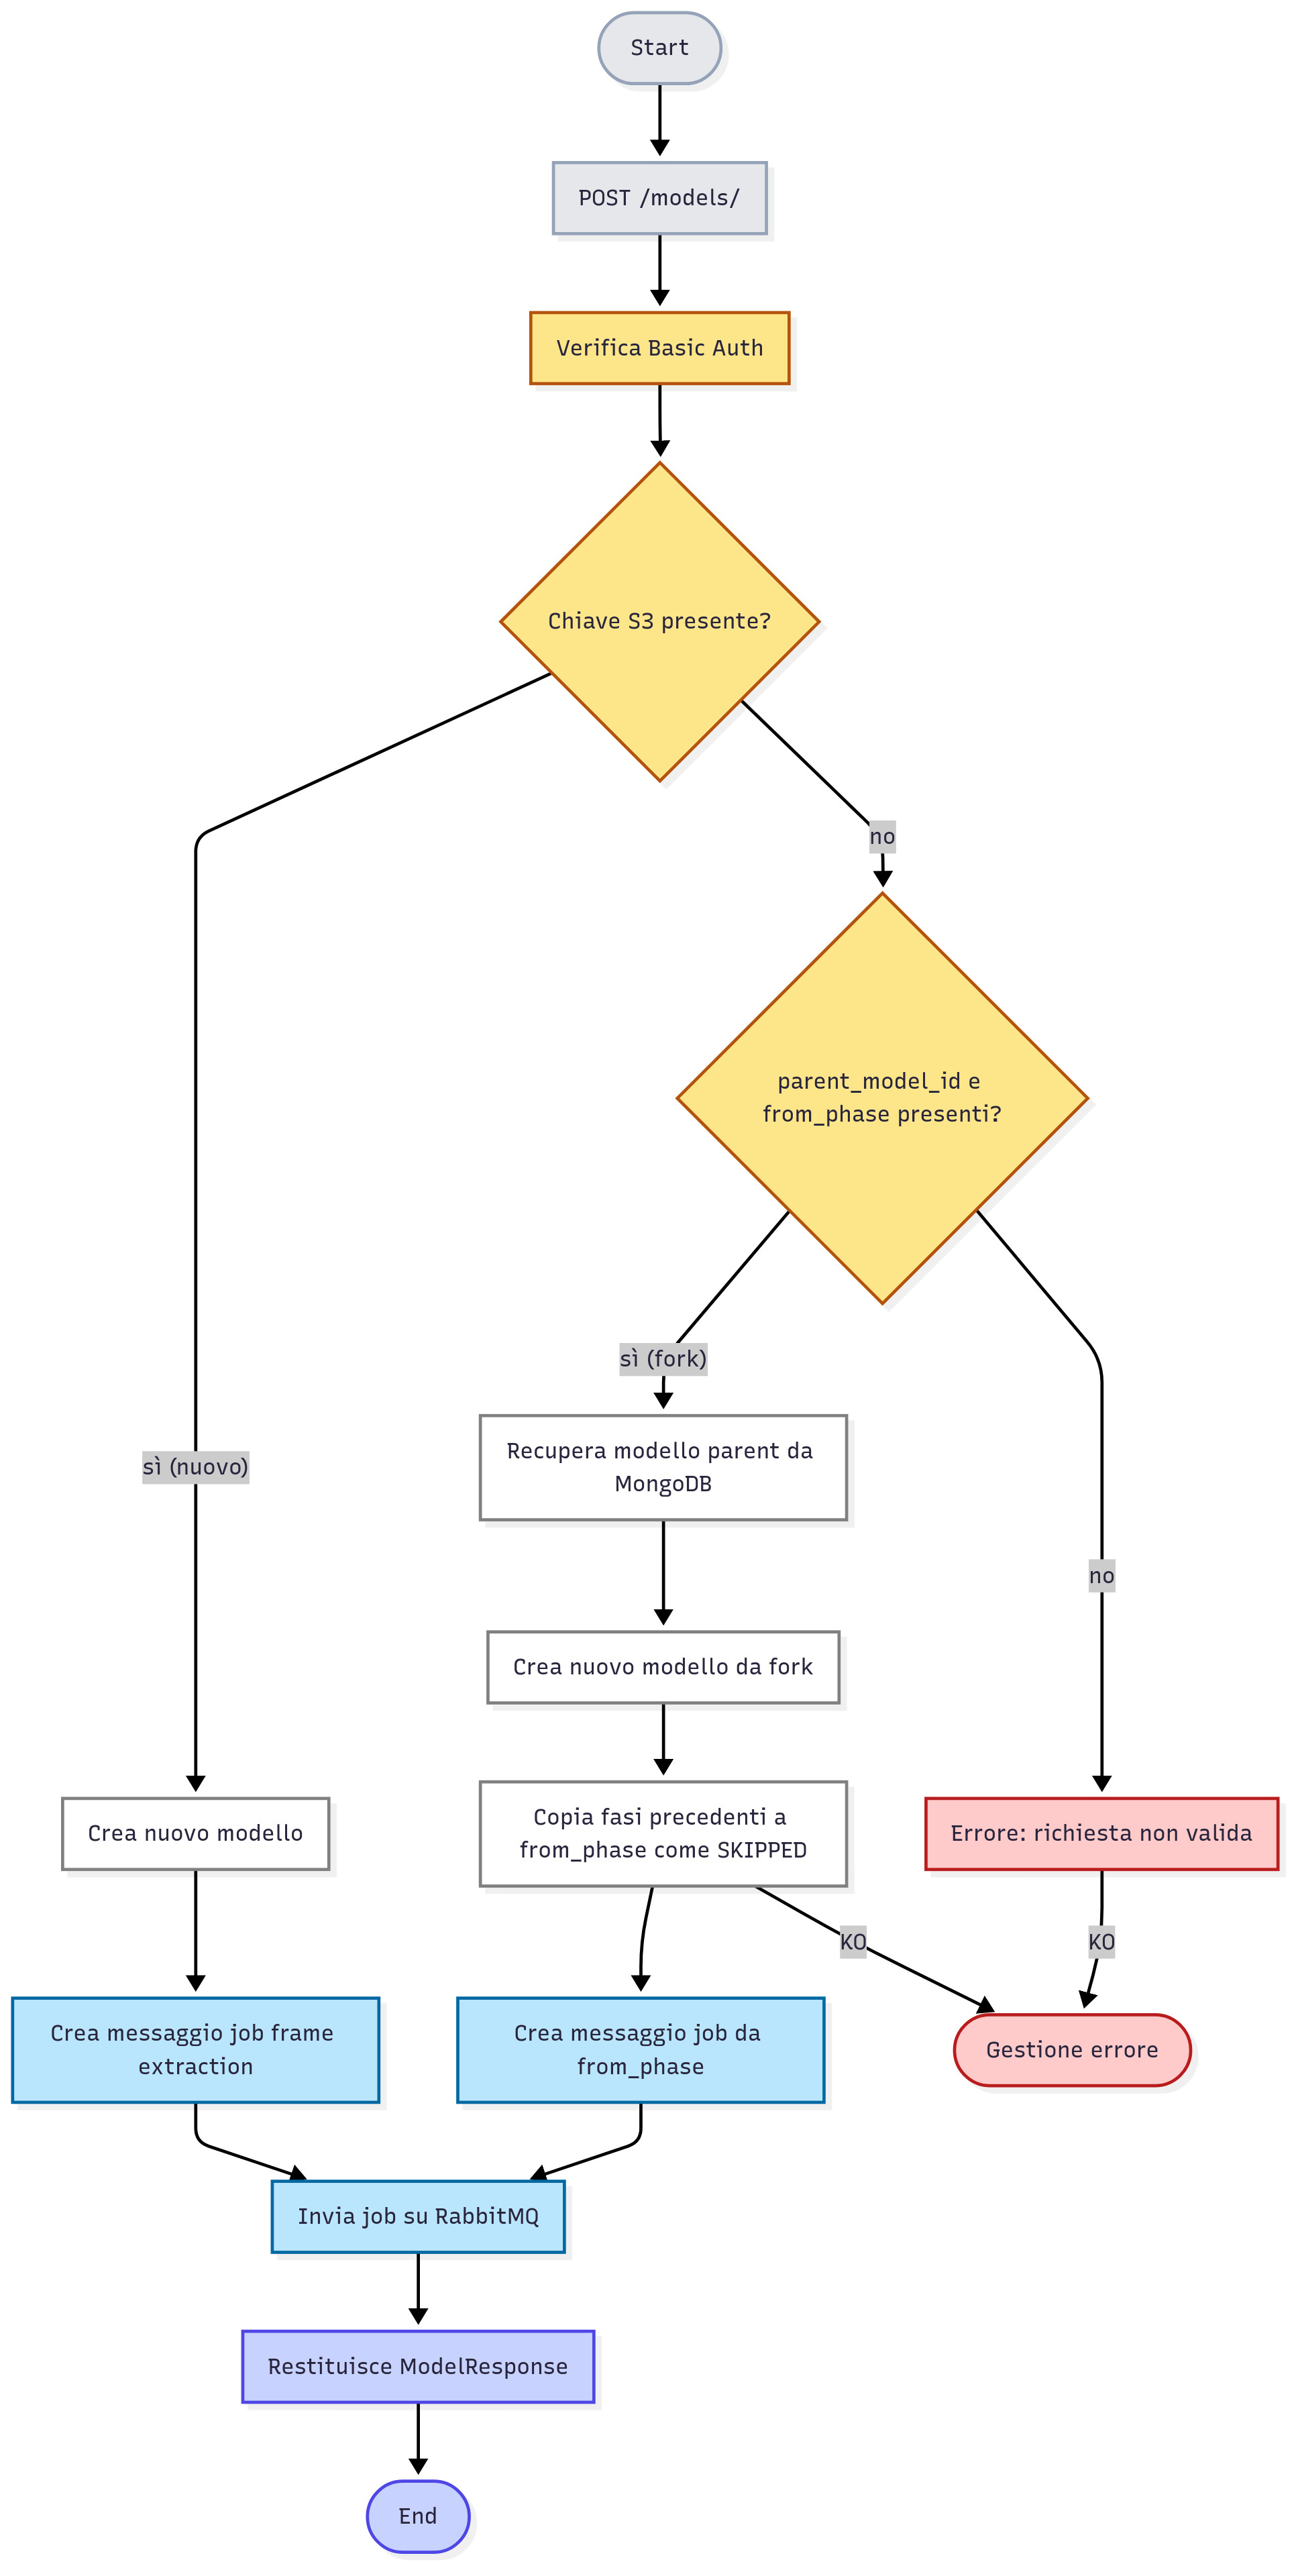
\includegraphics[width=0.5\textwidth]{images/create_or_fork_diagram.jpg}
	\caption{Diagramma per creazione e fork modello}
	\label{fig:create_or_fork_diagram}
\end{figure}

\begin{figure}[p]
	\centering
	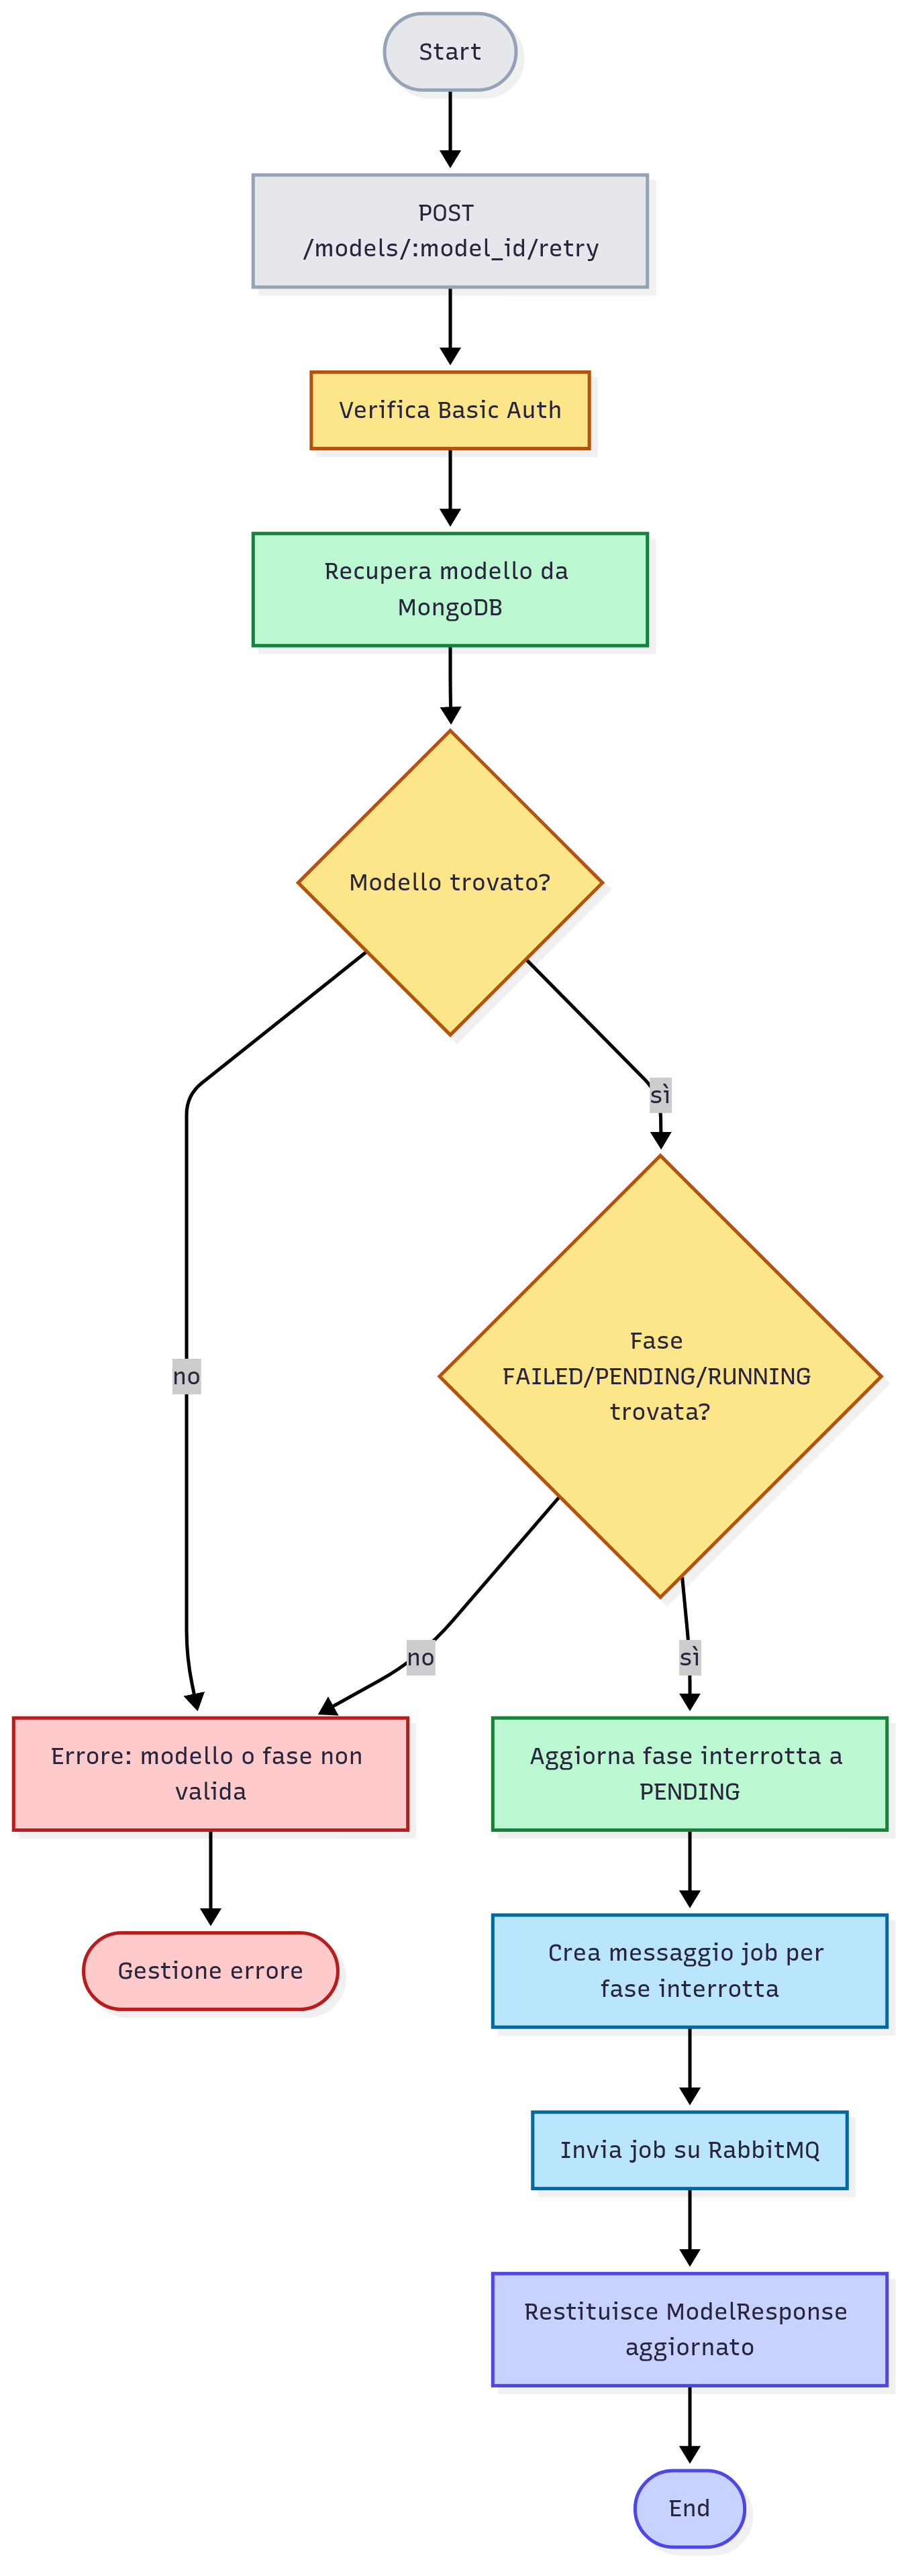
\includegraphics[width=0.5\textwidth]{images/retry_model_diagram.jpg}
	\caption{Diagramma per retry del modello}
	\label{fig:retry_diagram}
\end{figure}

\newpage
\subsection{Notifiche push in real-time}
Ogni volta che avviene un cambiamento rilevante nello stato dei modelli all’interno del database, il sistema è in grado di propagare in tempo reale una notifica ai client connessi. Dopo l’apertura della connessione WebSocket, il frontend riceve aggiornamenti direttamente dall’API Gateway, garantendo all’utente informazioni sempre aggiornate sull’avanzamento delle elaborazioni, senza la necessità di refresh manuali o polling periodico.

\begin{figure}[ht]
	\centering
	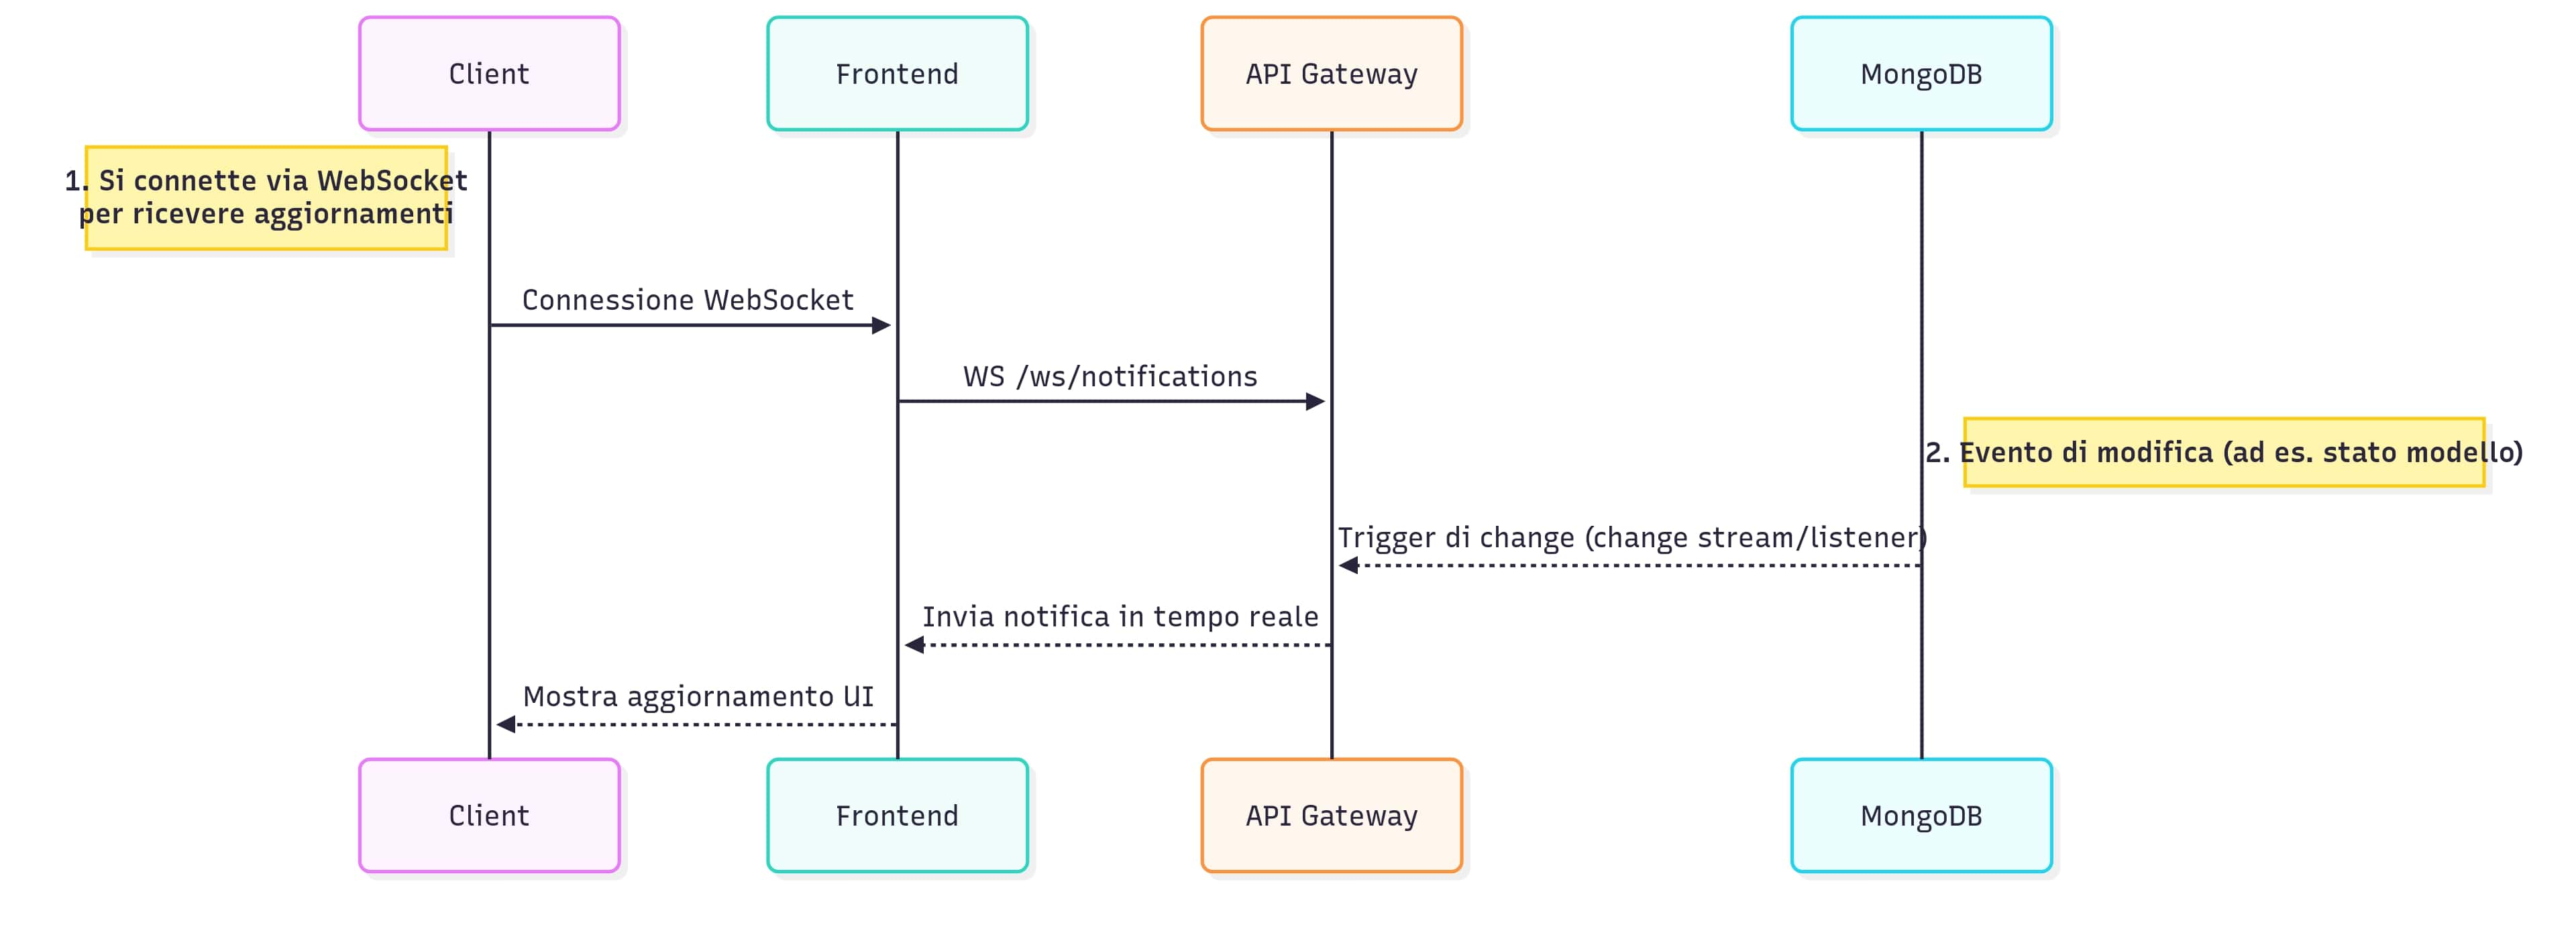
\includegraphics[width=0.9\textwidth]{images/push_notification_flow.jpg}
	\caption{Flusso per notifiche push in real-time}
	\label{fig:push_notification}
\end{figure}
\subsection{Considerazioni e Best Practice}

Il design di questo API Gateway consente di centralizzare la logica di business e la gestione della sicurezza, semplificando l’interazione tra frontend e servizi backend. La scelta di endpoint RESTful chiari, l’uso di WebSocket per le notifiche e l’integrazione di presigned URL per gli upload garantiscono \textbf{scalabilità, sicurezza e facilità d’integrazione}.


		


\section{Layer di Presentazione}

\subsection{Architettura dell'interfaccia utente}

Il frontend del sistema implementa un'interfaccia web moderna e responsiva progettata per rendere accessibile la tecnologia del 3D Gaussian Splatting a utenti non tecnici. L'applicazione, sviluppata con Vue.js 3 e Vuetify\footnote{https://vuetifyjs.com/en/}, offre un'esperienza utente coerente e intuitiva attraverso componenti Material Design ottimizzati per la gestione di workflow complessi.

\subsubsection{Dashboard Principale}

La dashboard rappresenta il punto di ingresso principale del sistema, organizzata secondo principi di information architecture che privilegiano la scansione rapida e l'accesso immediato alle funzionalità chiave. L'interfaccia adotta un layout a griglia responsivo che visualizza i modelli come card informative, ciascuna contenente:

\begin{itemize}
	\item \textbf{Preview thumbnail} del modello renderizzato, generata automaticamente alla conclusione della prima fase del workflow (estrazione dei frame).
	\item \textbf{Badge informativi} che comunicano immediatamente engine utilizzato (INRIA, MCMC, TAMING) e livello di qualità (Fast, Balanced, Quality)
	\item \textbf{Status indicator} con codifica cromatica per identificare rapidamente lo stato di elaborazione
	\item \textbf{Timeline di processing} che visualizza le cinque fasi del workflow con tempi di esecuzione individuali
	\item \textbf{Metriche di qualità} (PSNR, SSIM, LPIPS) presentate in formato espandibile per non sovraccaricare l'interfaccia
\end{itemize}

\begin{figure}[htbp]
	\centering
	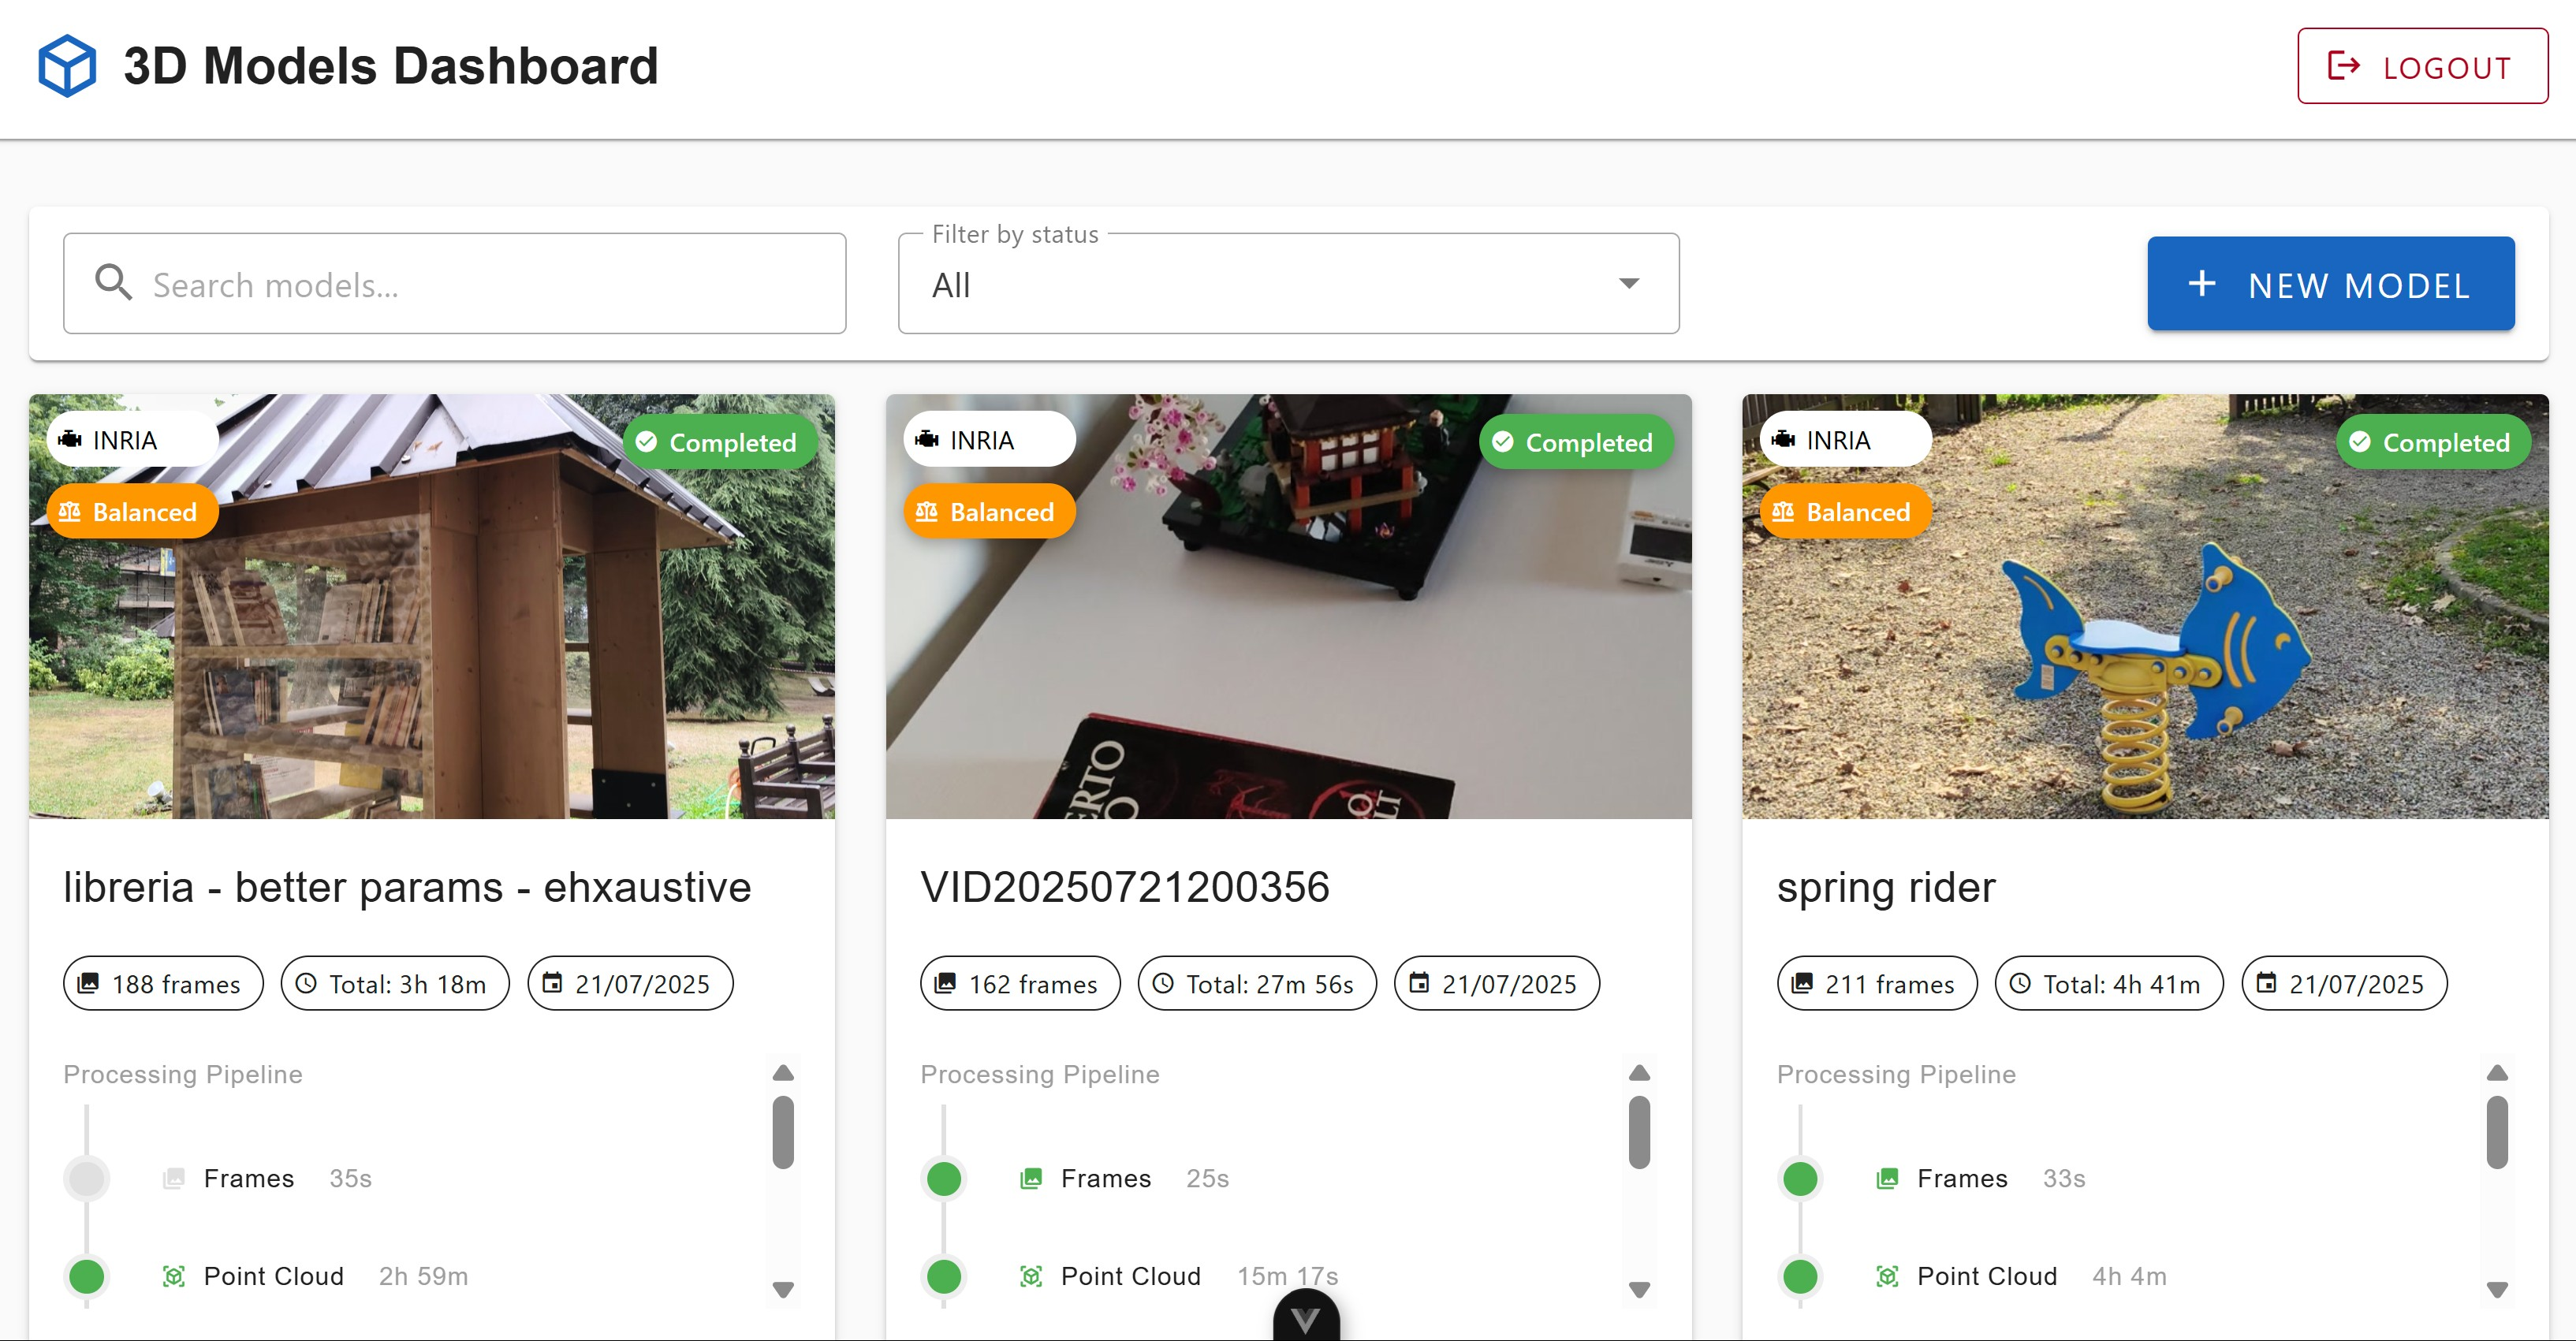
\includegraphics[width=\textwidth]{images/fronted_list.jpg}
	\caption{Dashboard principale con vista a griglia dei modelli, filtri di ricerca e indicatori di stato}
	\label{fig:dashboard_main}
\end{figure}

Il sistema di \textbf{filtraggio e ricerca} permette agli utenti di navigare efficacemente anche in presenza di centinaia di modelli, con filtri per stato, ricerca testuale e paginazione server-side che garantisce performance costanti indipendentemente dal volume di dati.

\subsubsection{Gestione del Workflow Utente}

L'interfaccia implementa tre modalità principali di creazione modelli, ciascuna ottimizzata per specifici scenari d'uso:

\paragraph{Creazione di un nuovo modello}
Il dialog di creazione nuovo modello guida l'utente attraverso un processo step-by-step che include:
\begin{itemize}
	\item Upload diretto del video tramite drag-and-drop o selezione file
	\item Configurazione intuitiva dei parametri attraverso slider visuali e card informative
	\item Preview real-time della pipeline di elaborazione che verrà eseguita
	\item Sistema di rating visuale per comunicare l'impatto delle scelte su velocità, qualità e requisiti hardware
\end{itemize}

\begin{figure}[htbp]
	\centering
	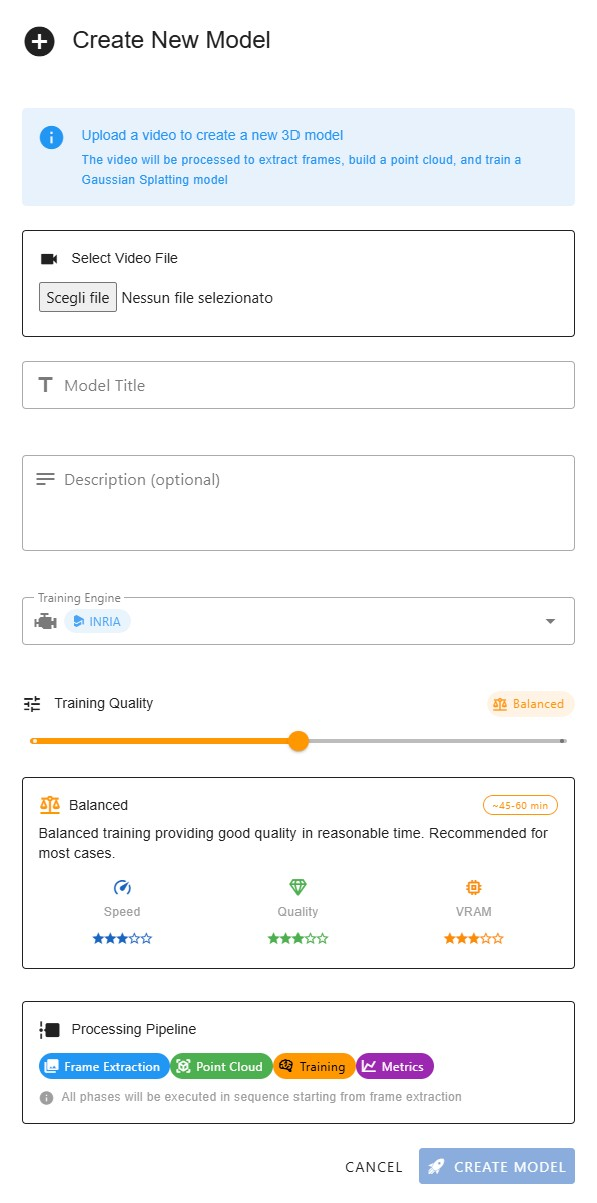
\includegraphics[width=0.7\textwidth]{images/fronted_new.jpg}
	\caption{Dialog di creazione nuovo modello con selezione engine e configurazione qualità tramite slider interattivo}
	\label{fig:new_model_dialog}
\end{figure}

\paragraph{Fork di un modello preesistente}
La funzionalità di fork permette di creare varianti di modelli esistenti riutilizzando fasi già completate. L'interfaccia visualizza chiaramente:
\begin{itemize}
	\item Quali fasi verranno riutilizzate (indicate con icona di cache)
	\item Da quale punto ripartirà l'elaborazione
	\item Stima del risparmio temporale rispetto a una nuova elaborazione completa
\end{itemize}

\begin{figure}[htbp]
	\centering
	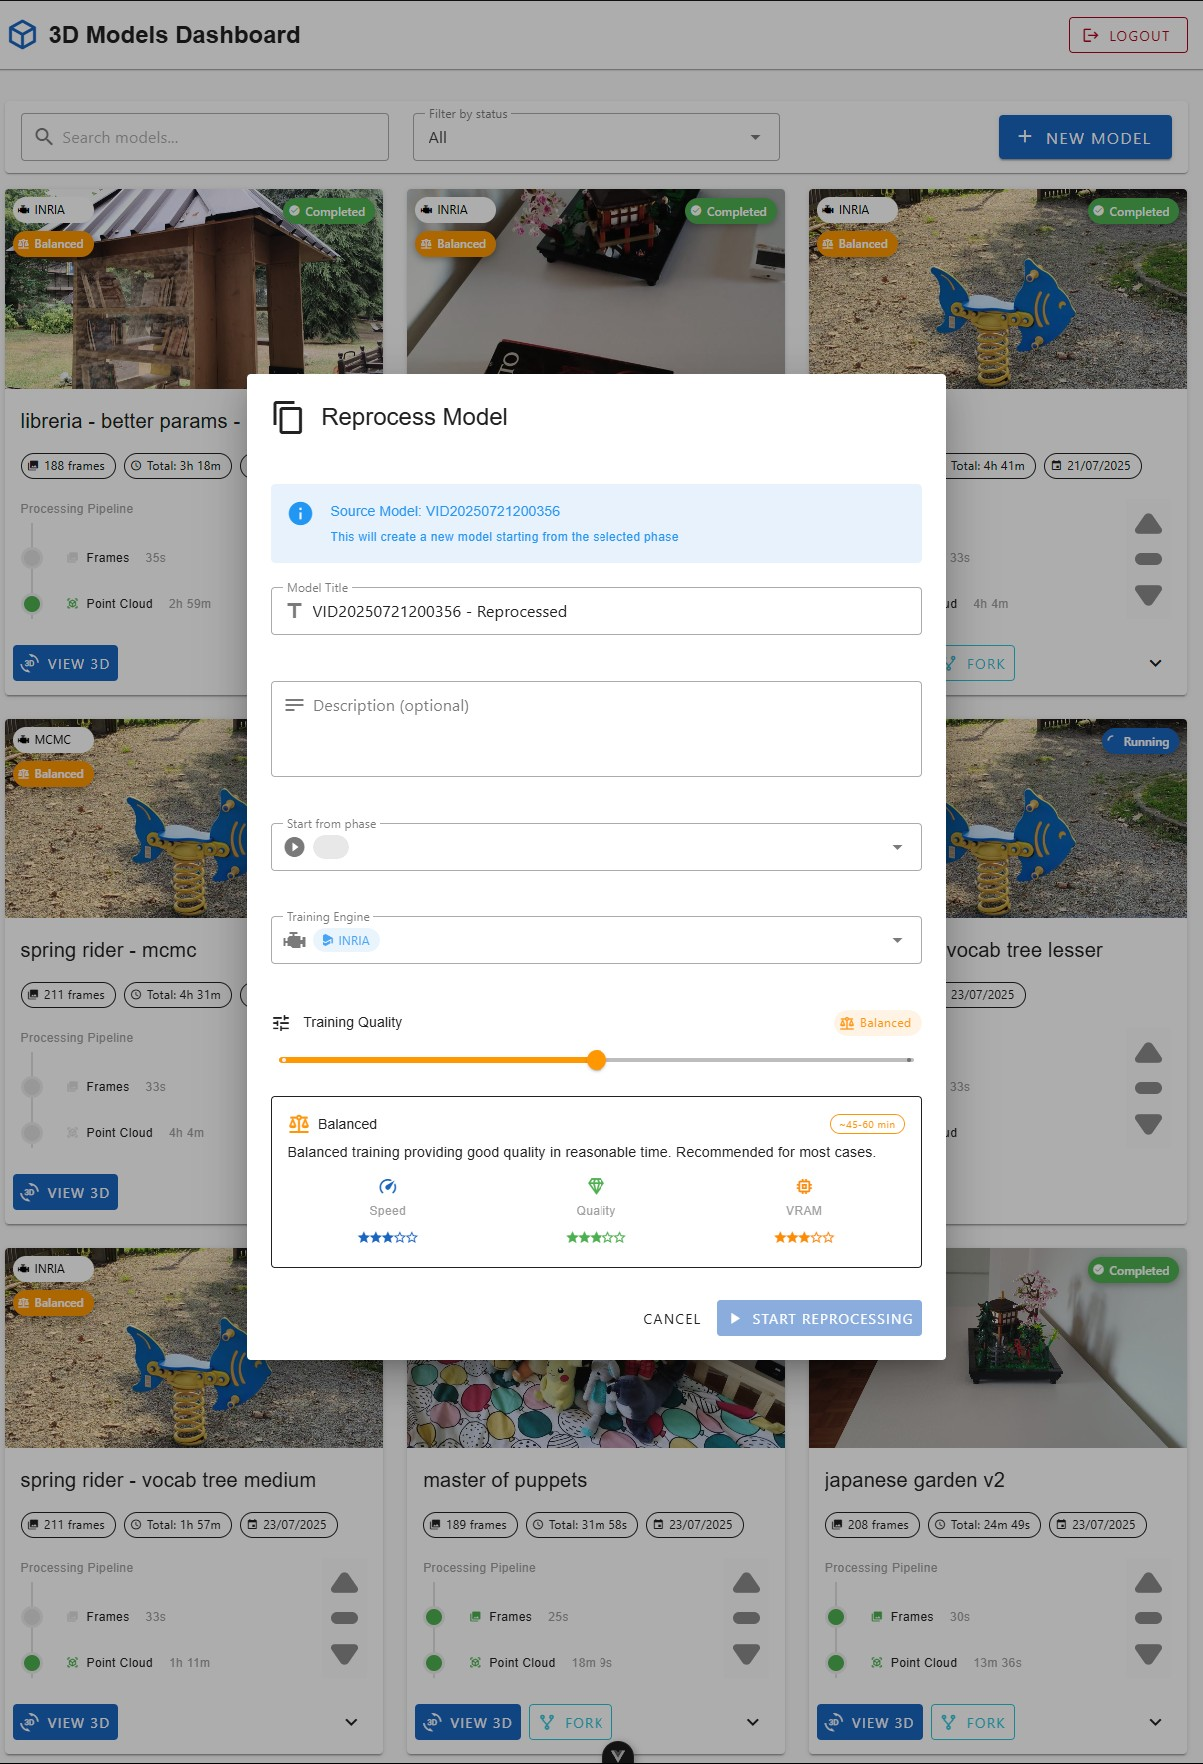
\includegraphics[width=0.8\textwidth]{images/frontend_fork.jpg}
	\caption{Dialog di reprocessing che mostra la selezione della fase di partenza e le fasi che verranno riutilizzate}
	\label{fig:fork_dialog}
\end{figure}

\paragraph{Retry intelligente}
Per modelli con elaborazione fallita, il sistema identifica automaticamente l'ultima fase completata con successo e propone di riprendere da quel punto, preservando il lavoro computazionale già svolto.

\subsection{Sistema di notifiche real-time}

Il frontend implementa un sofisticato sistema di notifiche basato su WebSocket che mantiene gli utenti informati sull'avanzamento delle elaborazioni senza richiedere refresh manuali della pagina.

\subsubsection{Architettura delle Notifiche}

Il sistema utilizza un approccio multi-livello per la gestione delle notifiche composto da:

\begin{itemize}
\item Toast Notifications: messaggi temporanei non invasivi che appaiono nell'angolo superiore destro per eventi chiave come completamento fasi o cambiamenti di stato. Ogni notifica è contestualizzata con icone e colori appropriati al tipo di evento.

\item  Notification Drawer:
un pannello laterale accessibile tramite FAB (Floating Action Button) che mantiene uno storico delle notifiche recenti. Il drawer implementa:
\begin{itemize}
	\item Raggruppamento intelligente per modello
	\item Indicatori di lettura/non lettura
	\item Timestamp relativi ("2 ore fa") per immediata comprensione temporale
	\item Azioni rapide per navigare al modello correlato
\end{itemize}

\begin{figure}[htbp]
	\centering
	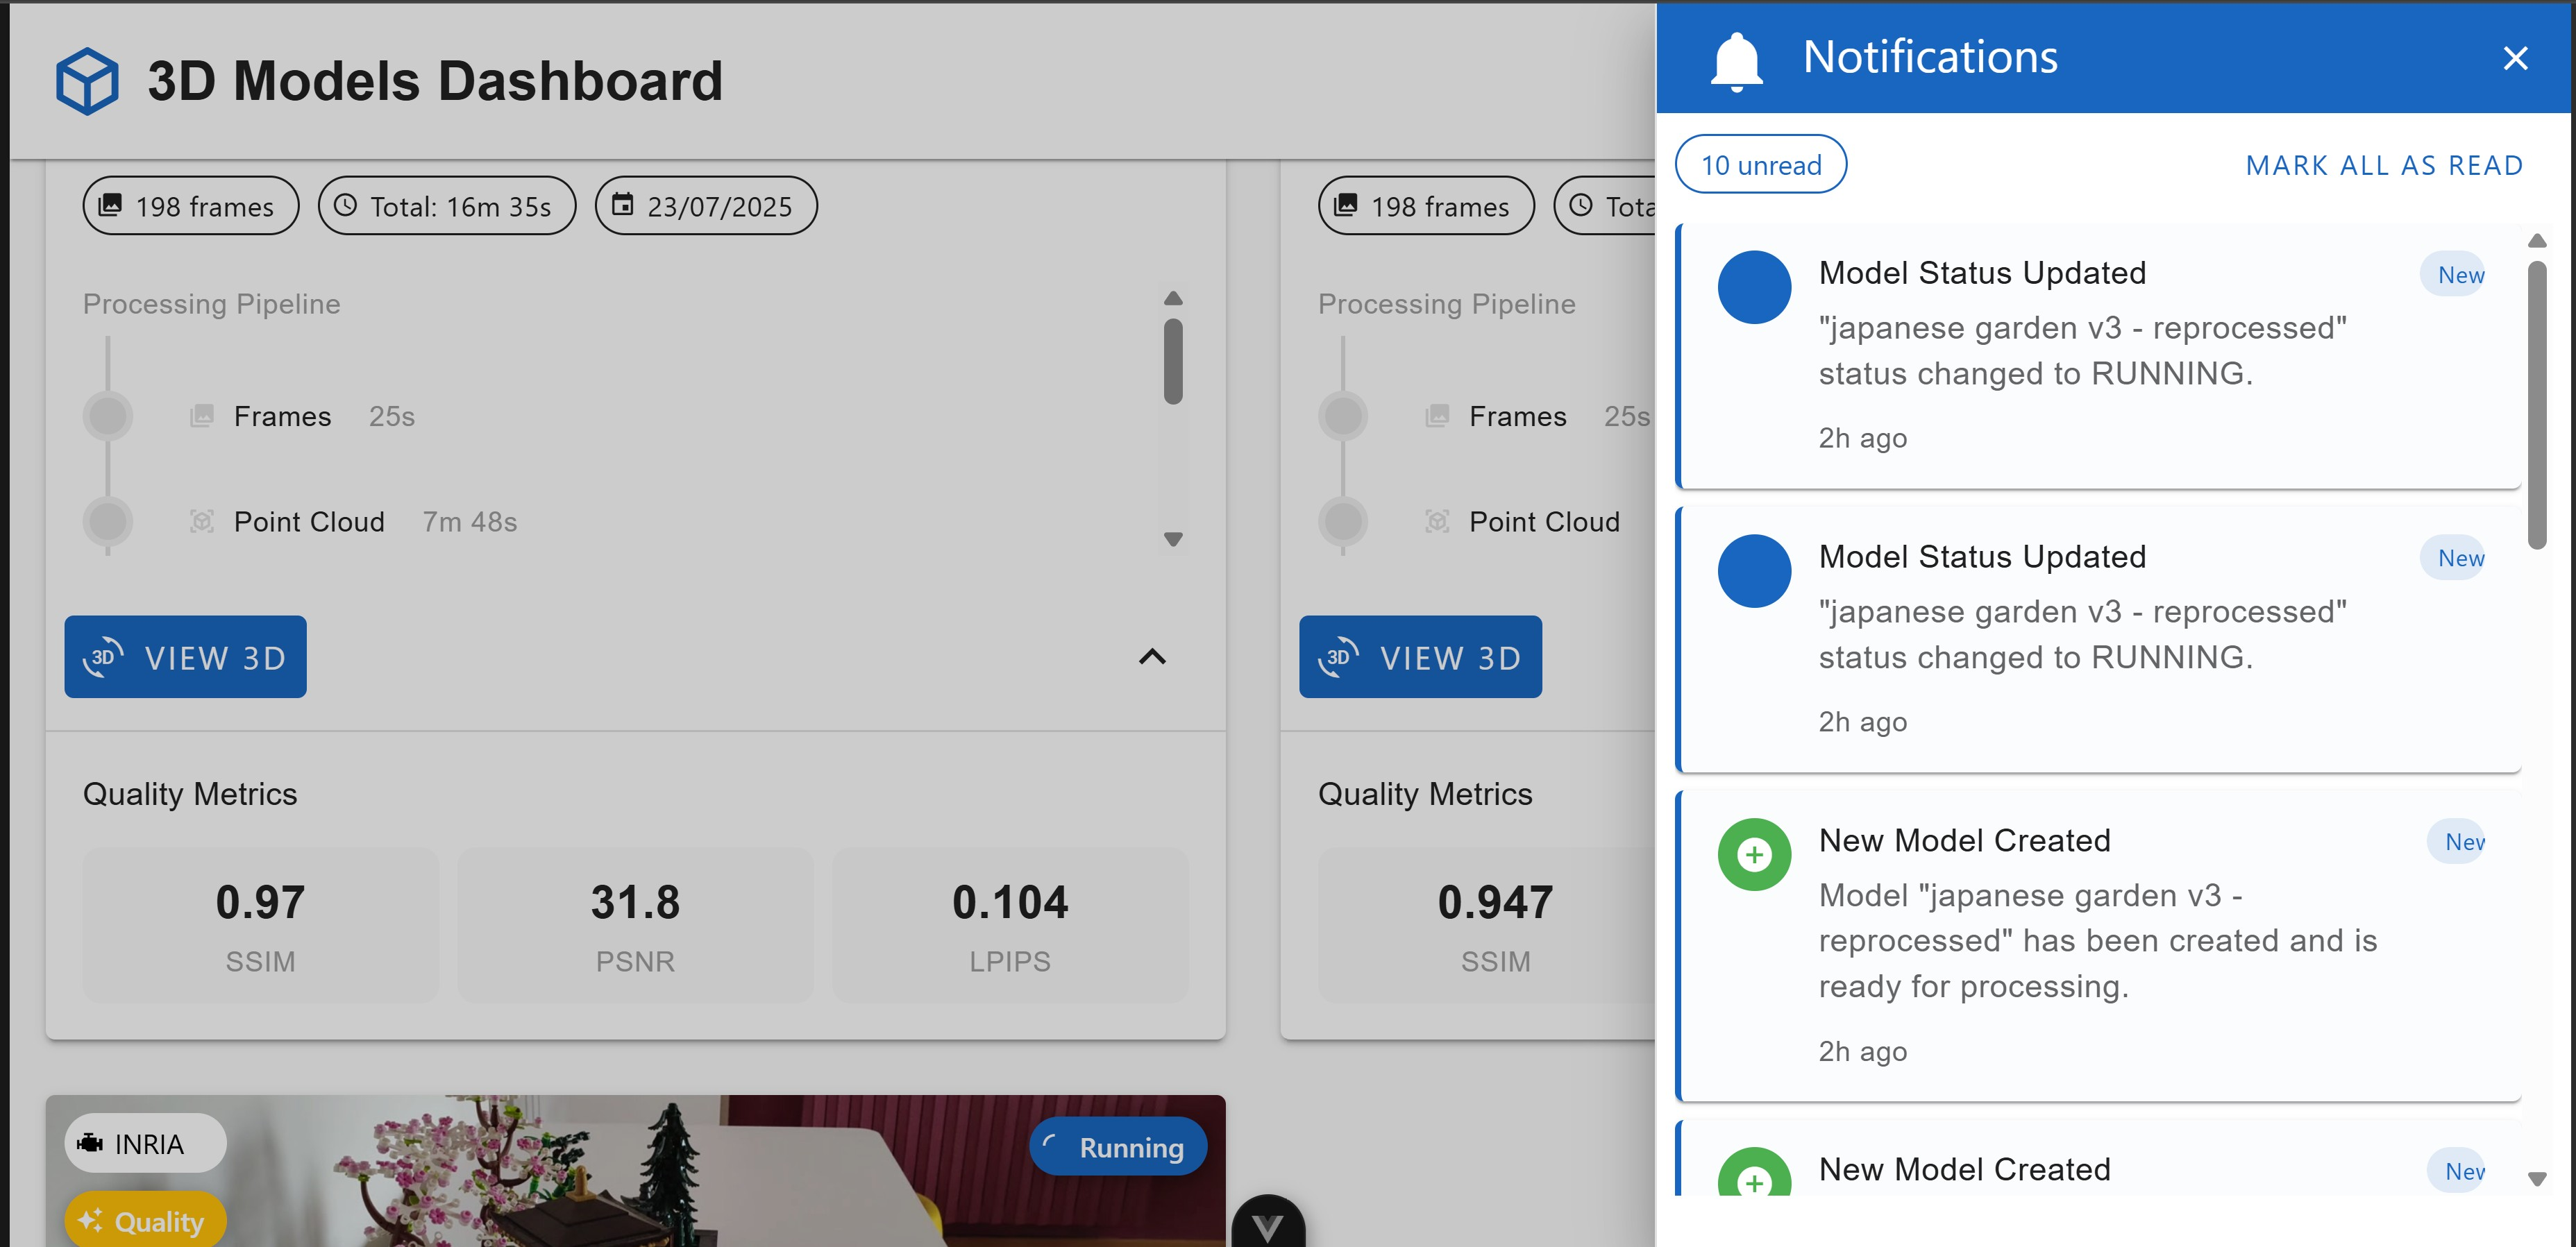
\includegraphics[width=0.9\textwidth]{images/frontend_notifications.jpg}
	\caption{Sistema di notifiche con drawer laterale che mostra lo storico degli eventi e badge per notifiche non lette}
	\label{fig:notification_drawer}
\end{figure}

\item Live Updates
La dashboard si aggiorna automaticamente quando arrivano notifiche relative a modelli visibili nella pagina corrente, eliminando la necessità di polling manuale e garantendo che le informazioni visualizzate siano sempre aggiornate.
\end{itemize}
\subsubsection{Gestione stati di connessione}
Il sistema monitora costantemente lo stato della connessione WebSocket, fornendo feedback visuale quando la connessione viene persa e implementando meccanismi di riconnessione automatica con backoff esponenziale per gestire interruzioni temporanee di rete.

\begin{figure}[htbp]
	\centering
	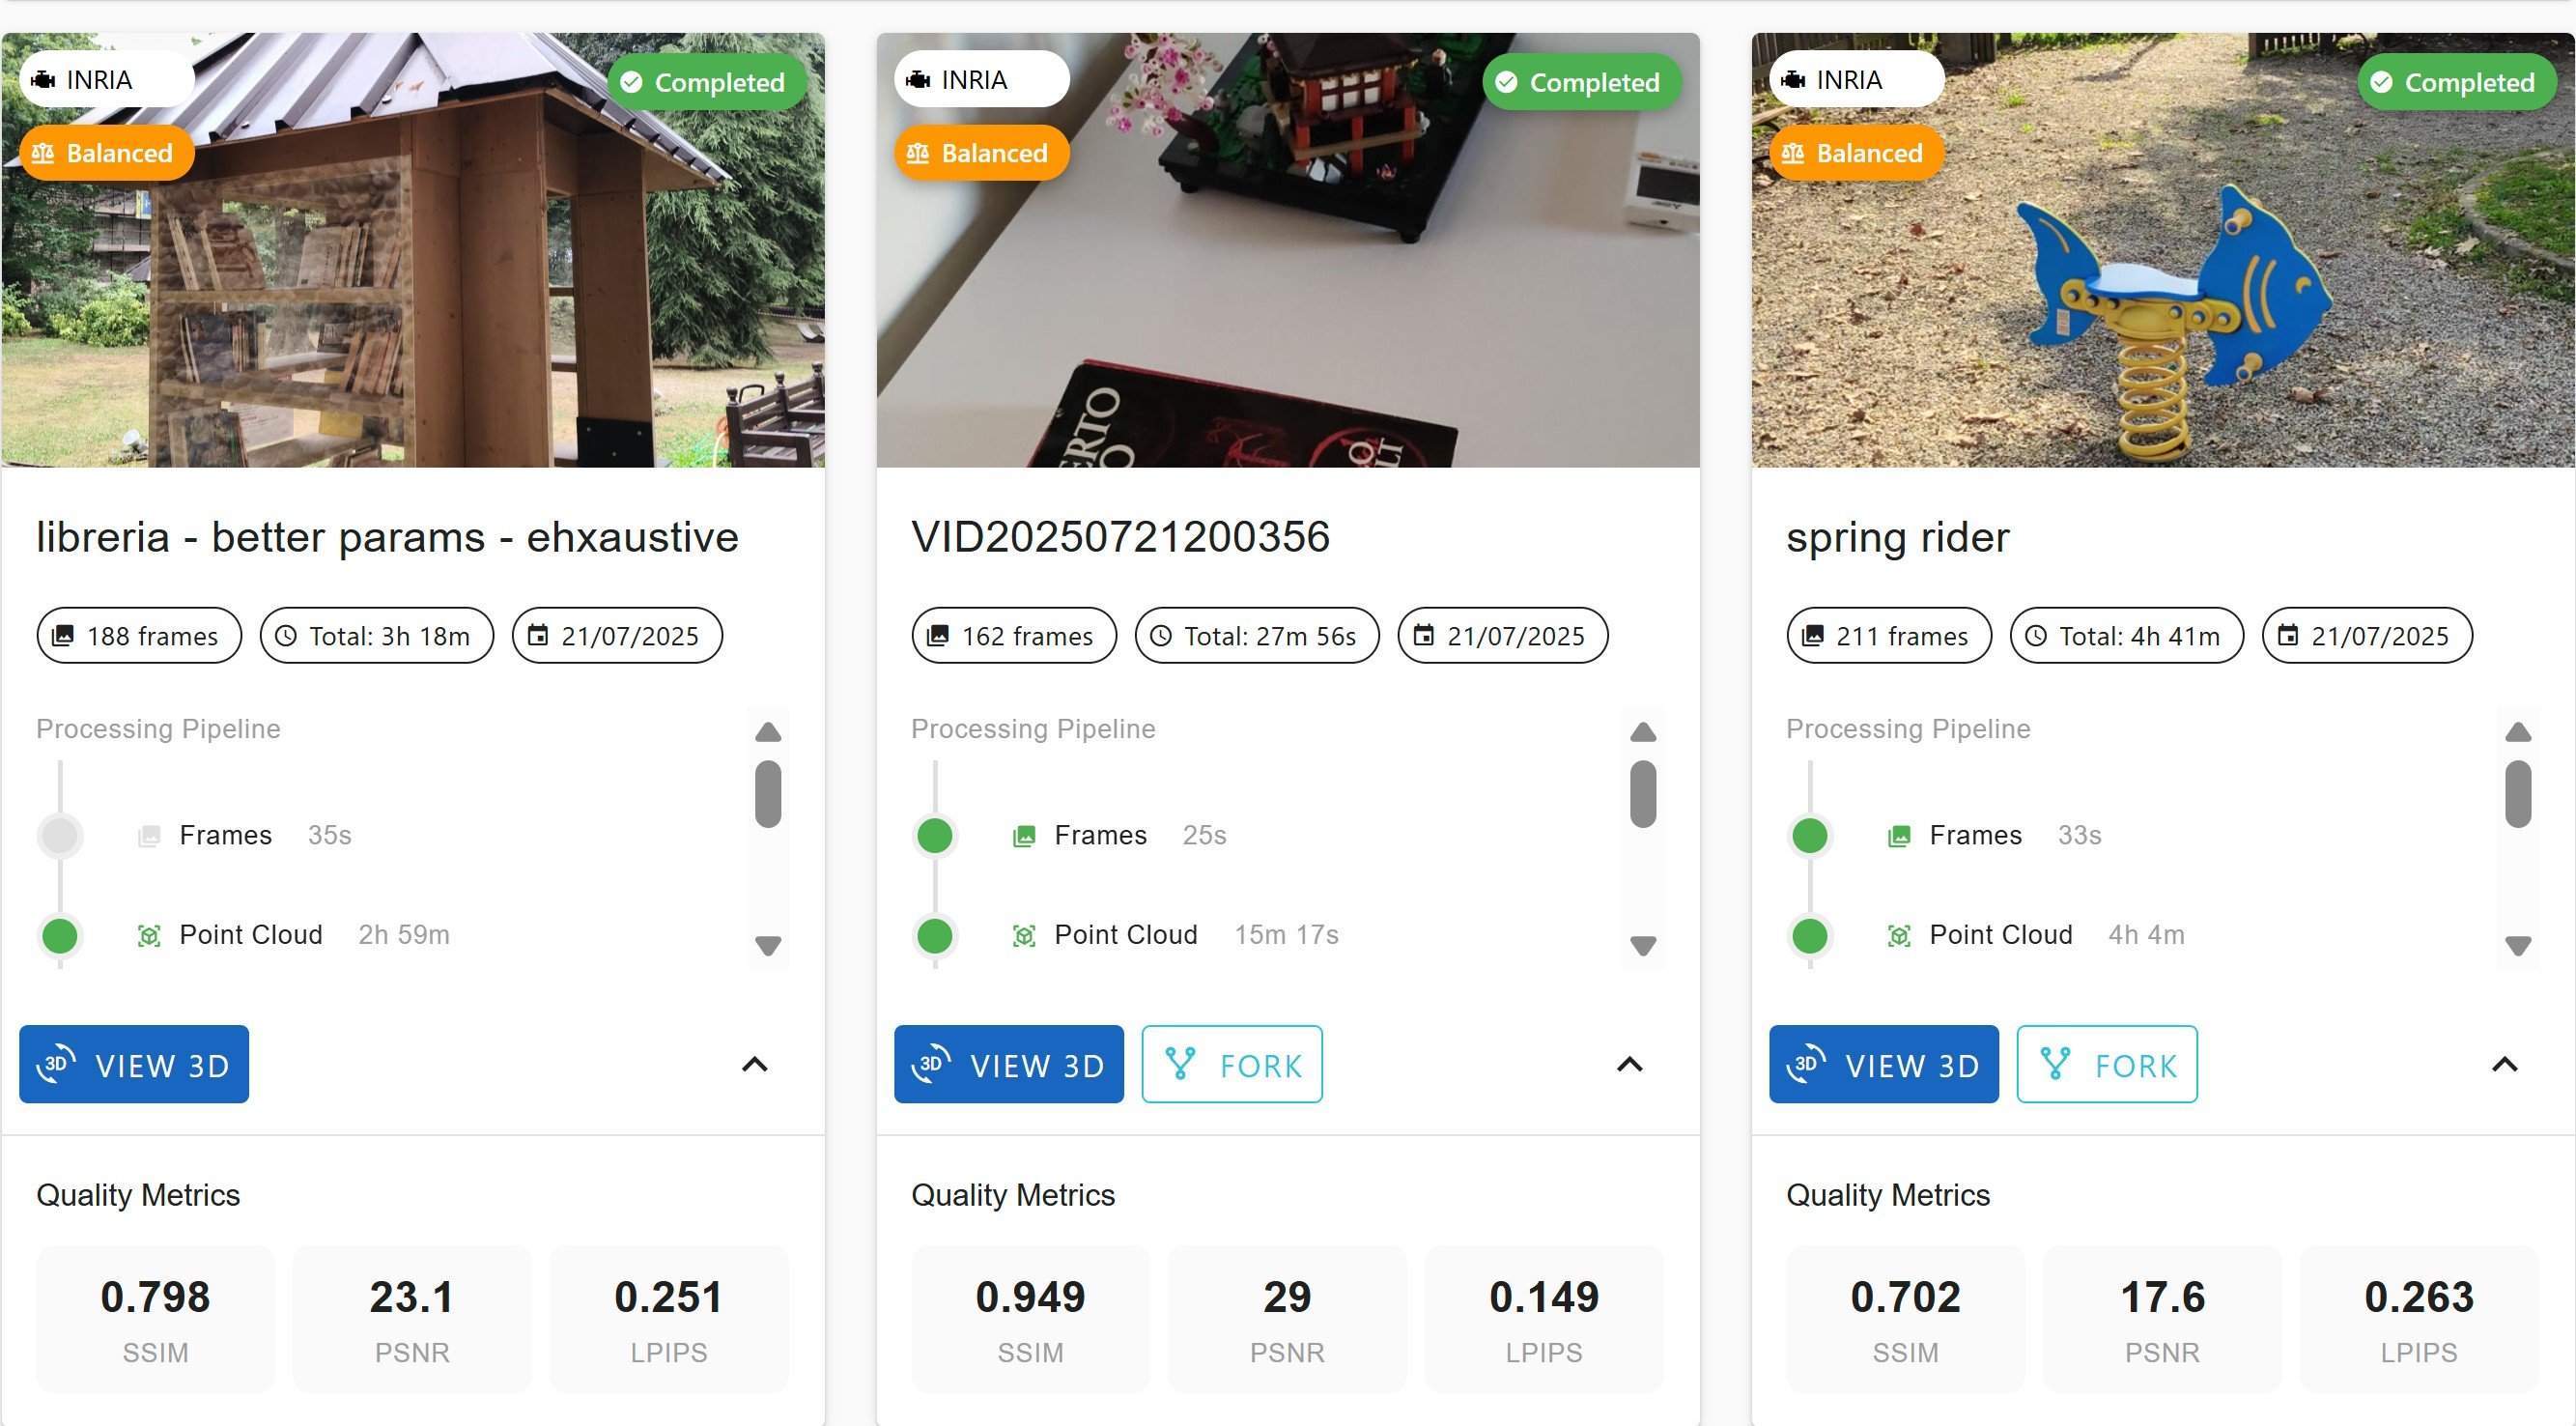
\includegraphics[width=\textwidth]{images/frontend_show_metrics.jpg}
	\caption{Vista espansa delle metriche di qualità (SSIM, PSNR, LPIPS) per confronto rapido tra modelli}
	\label{fig:dashboard_metrics}
\end{figure}

\subsection{Visualizzatore 3D Integrato}

Il componente di visualizzazione 3D rappresenta il culmine dell'esperienza utente, permettendo l'esplorazione interattiva dei modelli generati direttamente nel browser.

\subsubsection{Tecnologia di Rendering}

Il viewer utilizza la libreria \textbf{GaussianSplats3D} basata su Three.js, specificamente ottimizzata per il rendering efficiente di primitive gaussiane. Questa scelta tecnologica garantisce:

\begin{itemize}
	\item \textbf{Performance real-time}: Rendering a 60 FPS anche per modelli con centinaia di migliaia di splat
	\item \textbf{Compatibilità cross-platform}: Funzionamento su qualsiasi dispositivo con supporto WebGL
	\item \textbf{Interattività fluida}: Controlli camera intuitivi per rotazione, zoom e pan
\end{itemize}

\subsubsection{Interfaccia del Viewer}

Il viewer 3D implementa un'interfaccia minimalista che massimizza l'area di visualizzazione mantenendo accessibili le informazioni essenziali:

\paragraph{Overlay Informativo}
Un pannello semi-trasparente nell'angolo superiore sinistro visualizza:
\begin{itemize}
	\item Statistiche di rendering (FPS, numero di splat)
	\item Metriche di qualità del modello
	\item Engine e parametri utilizzati per il training
\end{itemize}

\begin{figure}[htbp]
	\centering
	\begin{subfigure}[b]{0.49\textwidth}
		\centering
		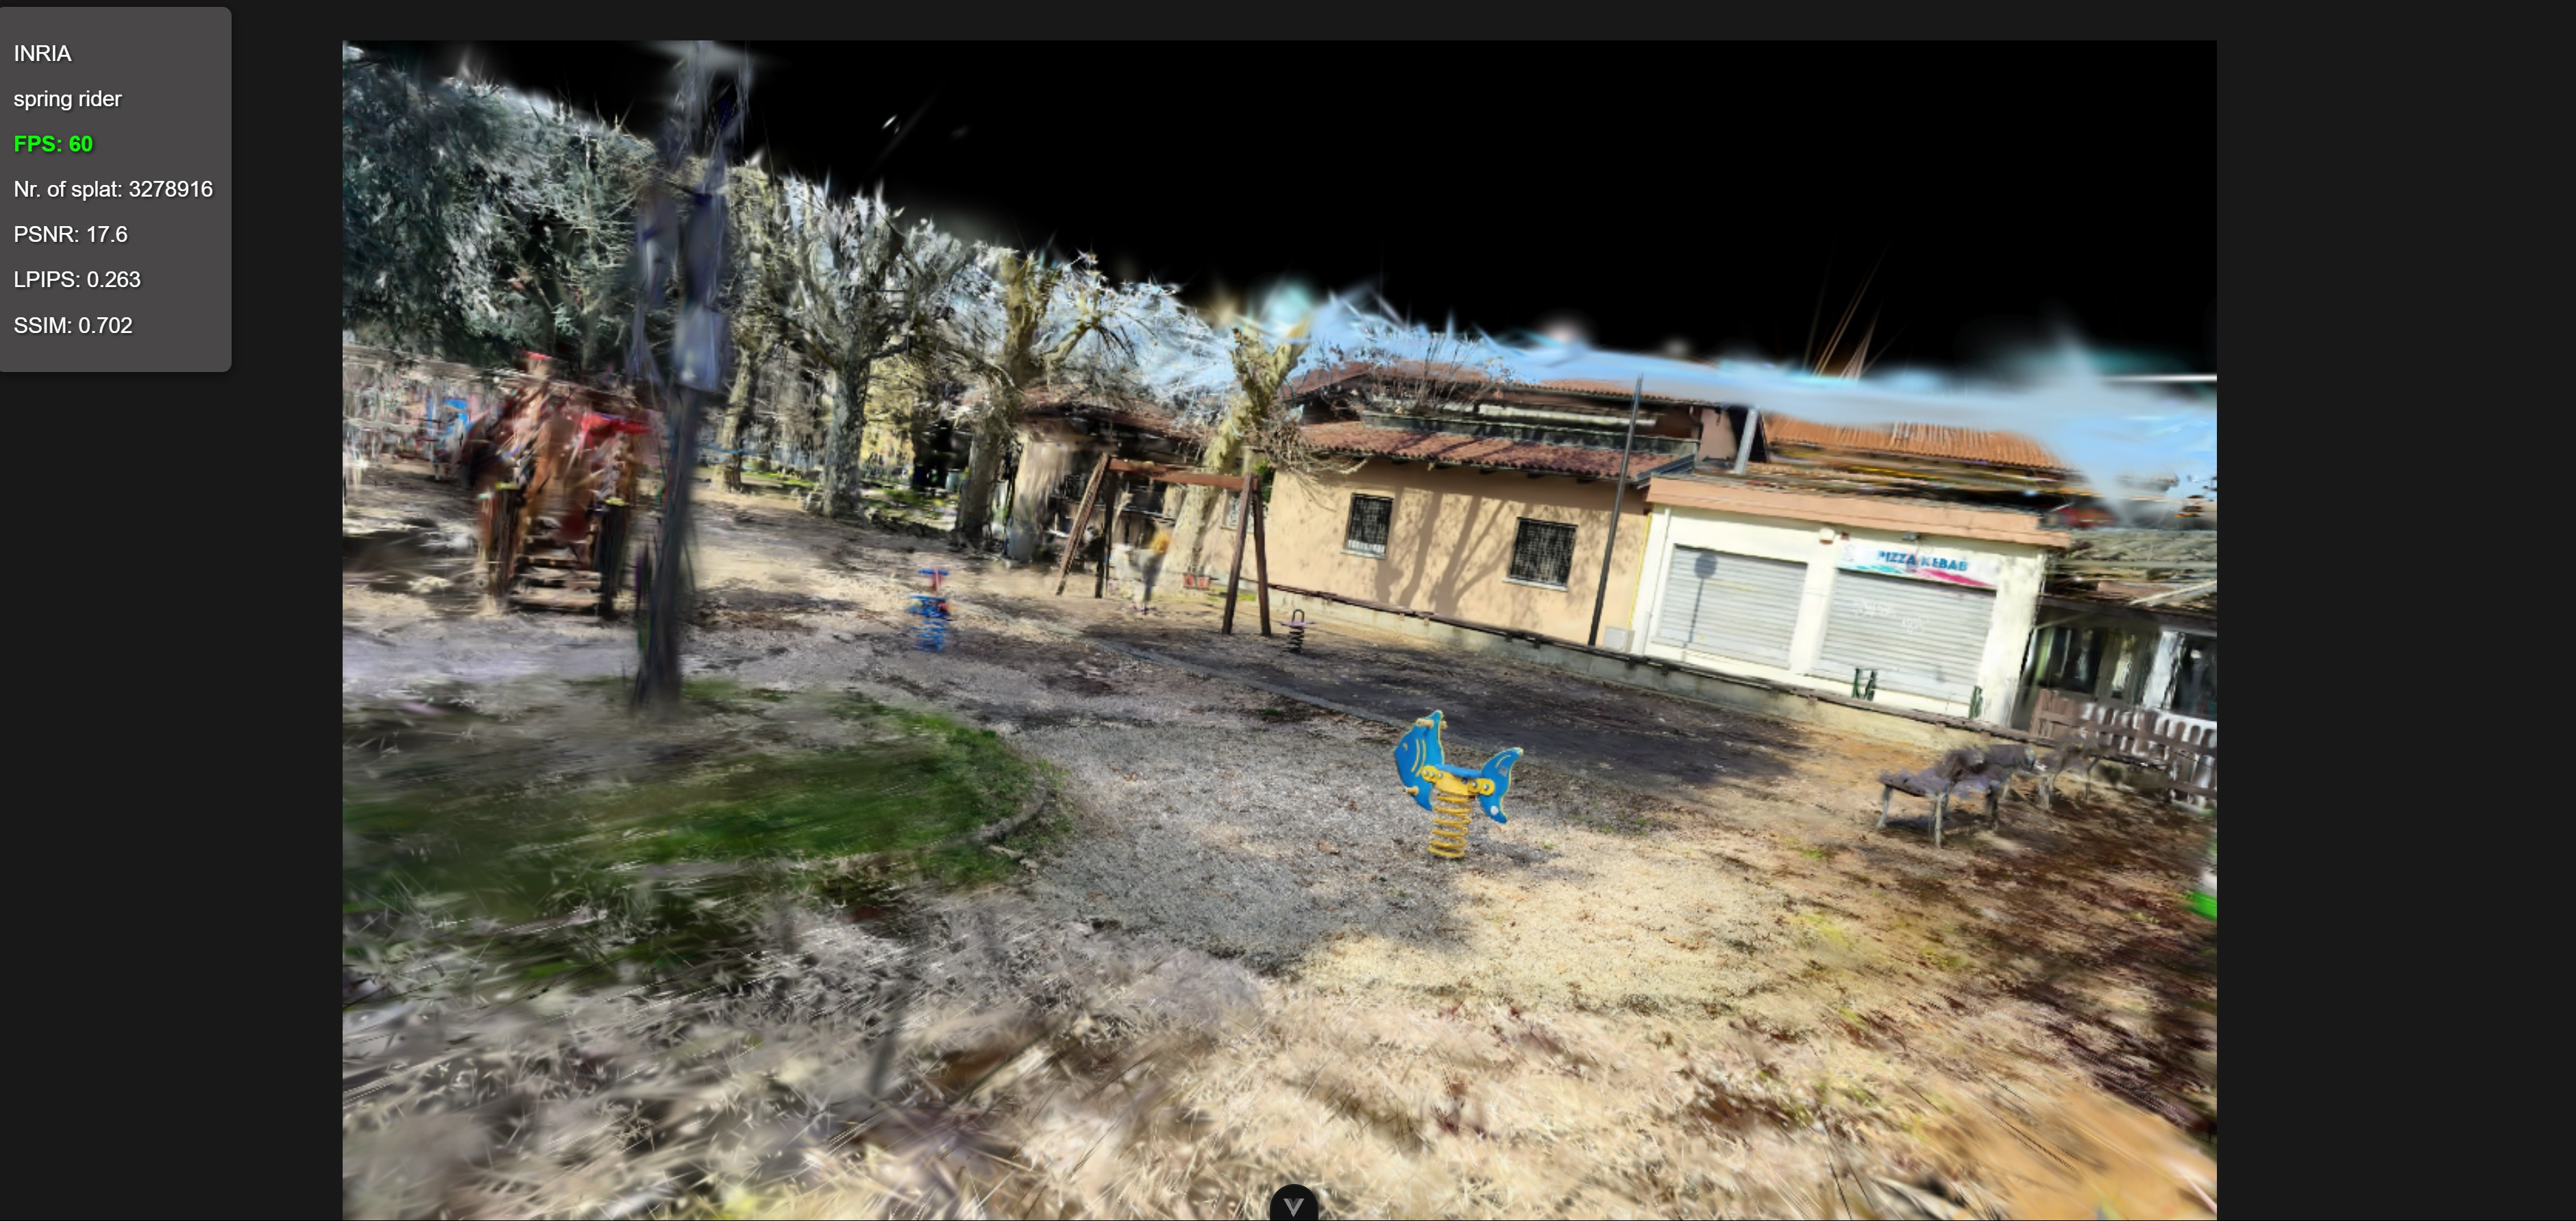
\includegraphics[width=\textwidth]{images/frontend_viewer.jpg}
		\caption{Spring rider - 327k splats}
	\end{subfigure}
	\hfill
	\begin{subfigure}[b]{0.49\textwidth}
		\centering
		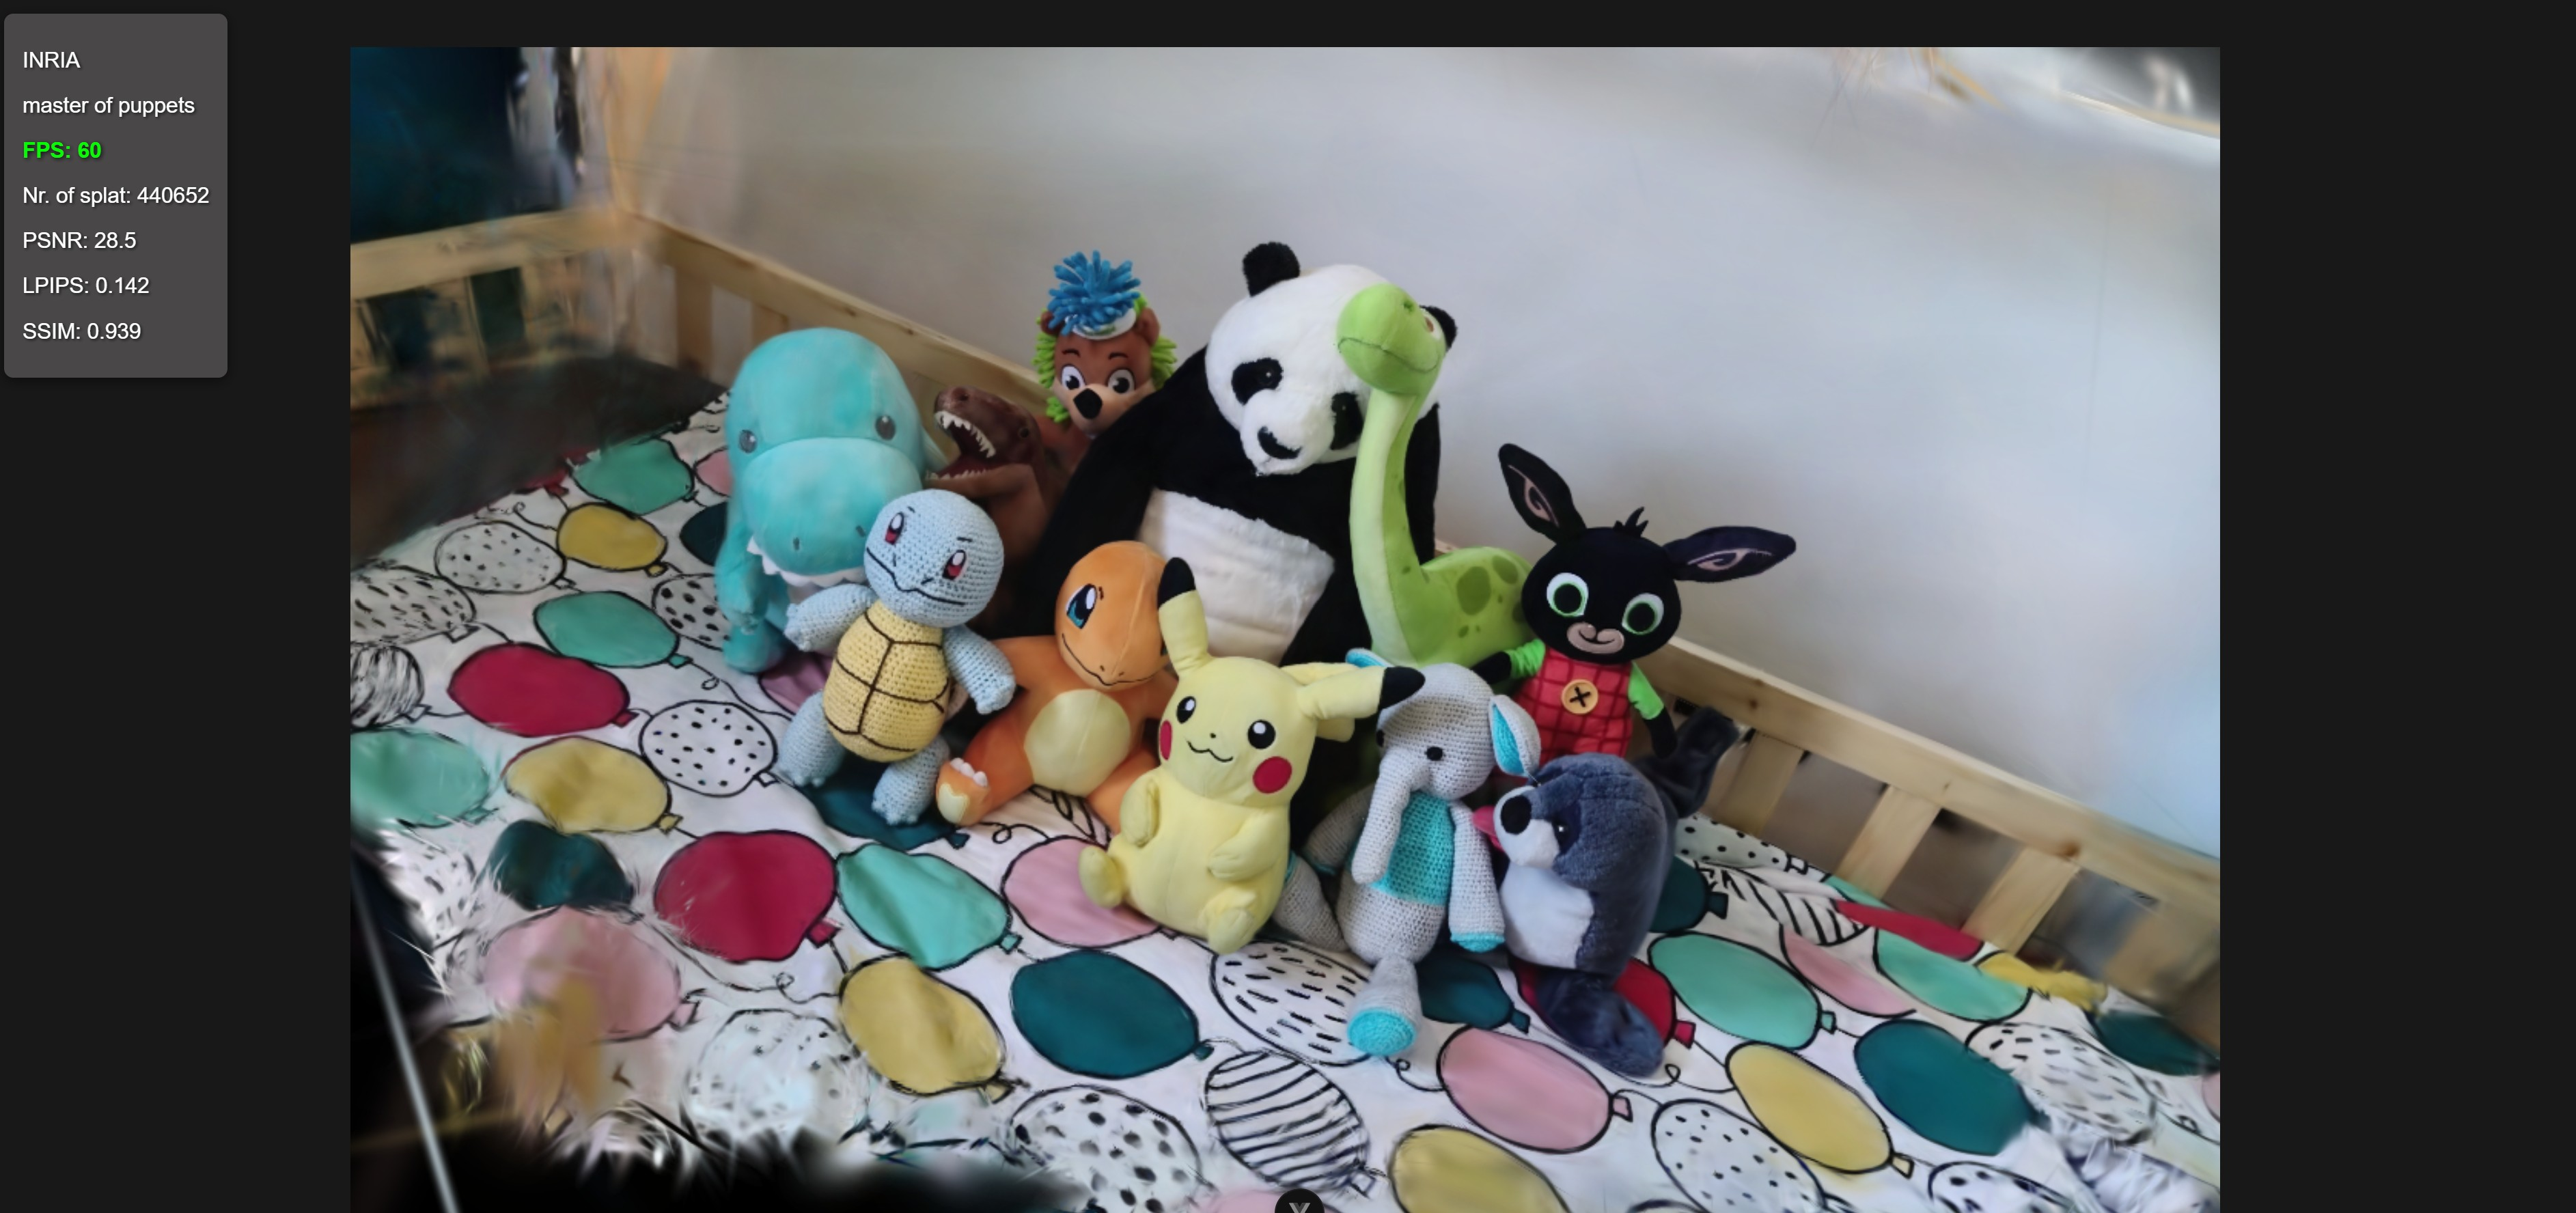
\includegraphics[width=\textwidth]{images/frontend_viewer_2.jpg}
		\caption{Master of puppets - 440k splats}
	\end{subfigure}
	\caption{Visualizzatore 3D integrato con overlay informativo mostrante FPS, numero di splat e metriche di qualità}
	\label{fig:viewer3d_examples}
\end{figure}

\paragraph{Controlli Camera}
Il sistema recupera automaticamente la posizione camera ottimale dal dataset di training, garantendo che il modello sia presentato dalla prospettiva più favorevole al primo caricamento. Gli utenti possono poi esplorare liberamente utilizzando controlli standard di navigazione 3D.

\paragraph{Gestione formati}
Il viewer gestisce trasparentemente la conversione tra formati, accettando sia file PLY che SPLAT ottimizzati e applicando le trasformazioni necessarie per la corretta visualizzazione, incluse conversioni di opacità specifiche per diversi algoritmi di training.

\begin{figure}[htbp]
	\centering
	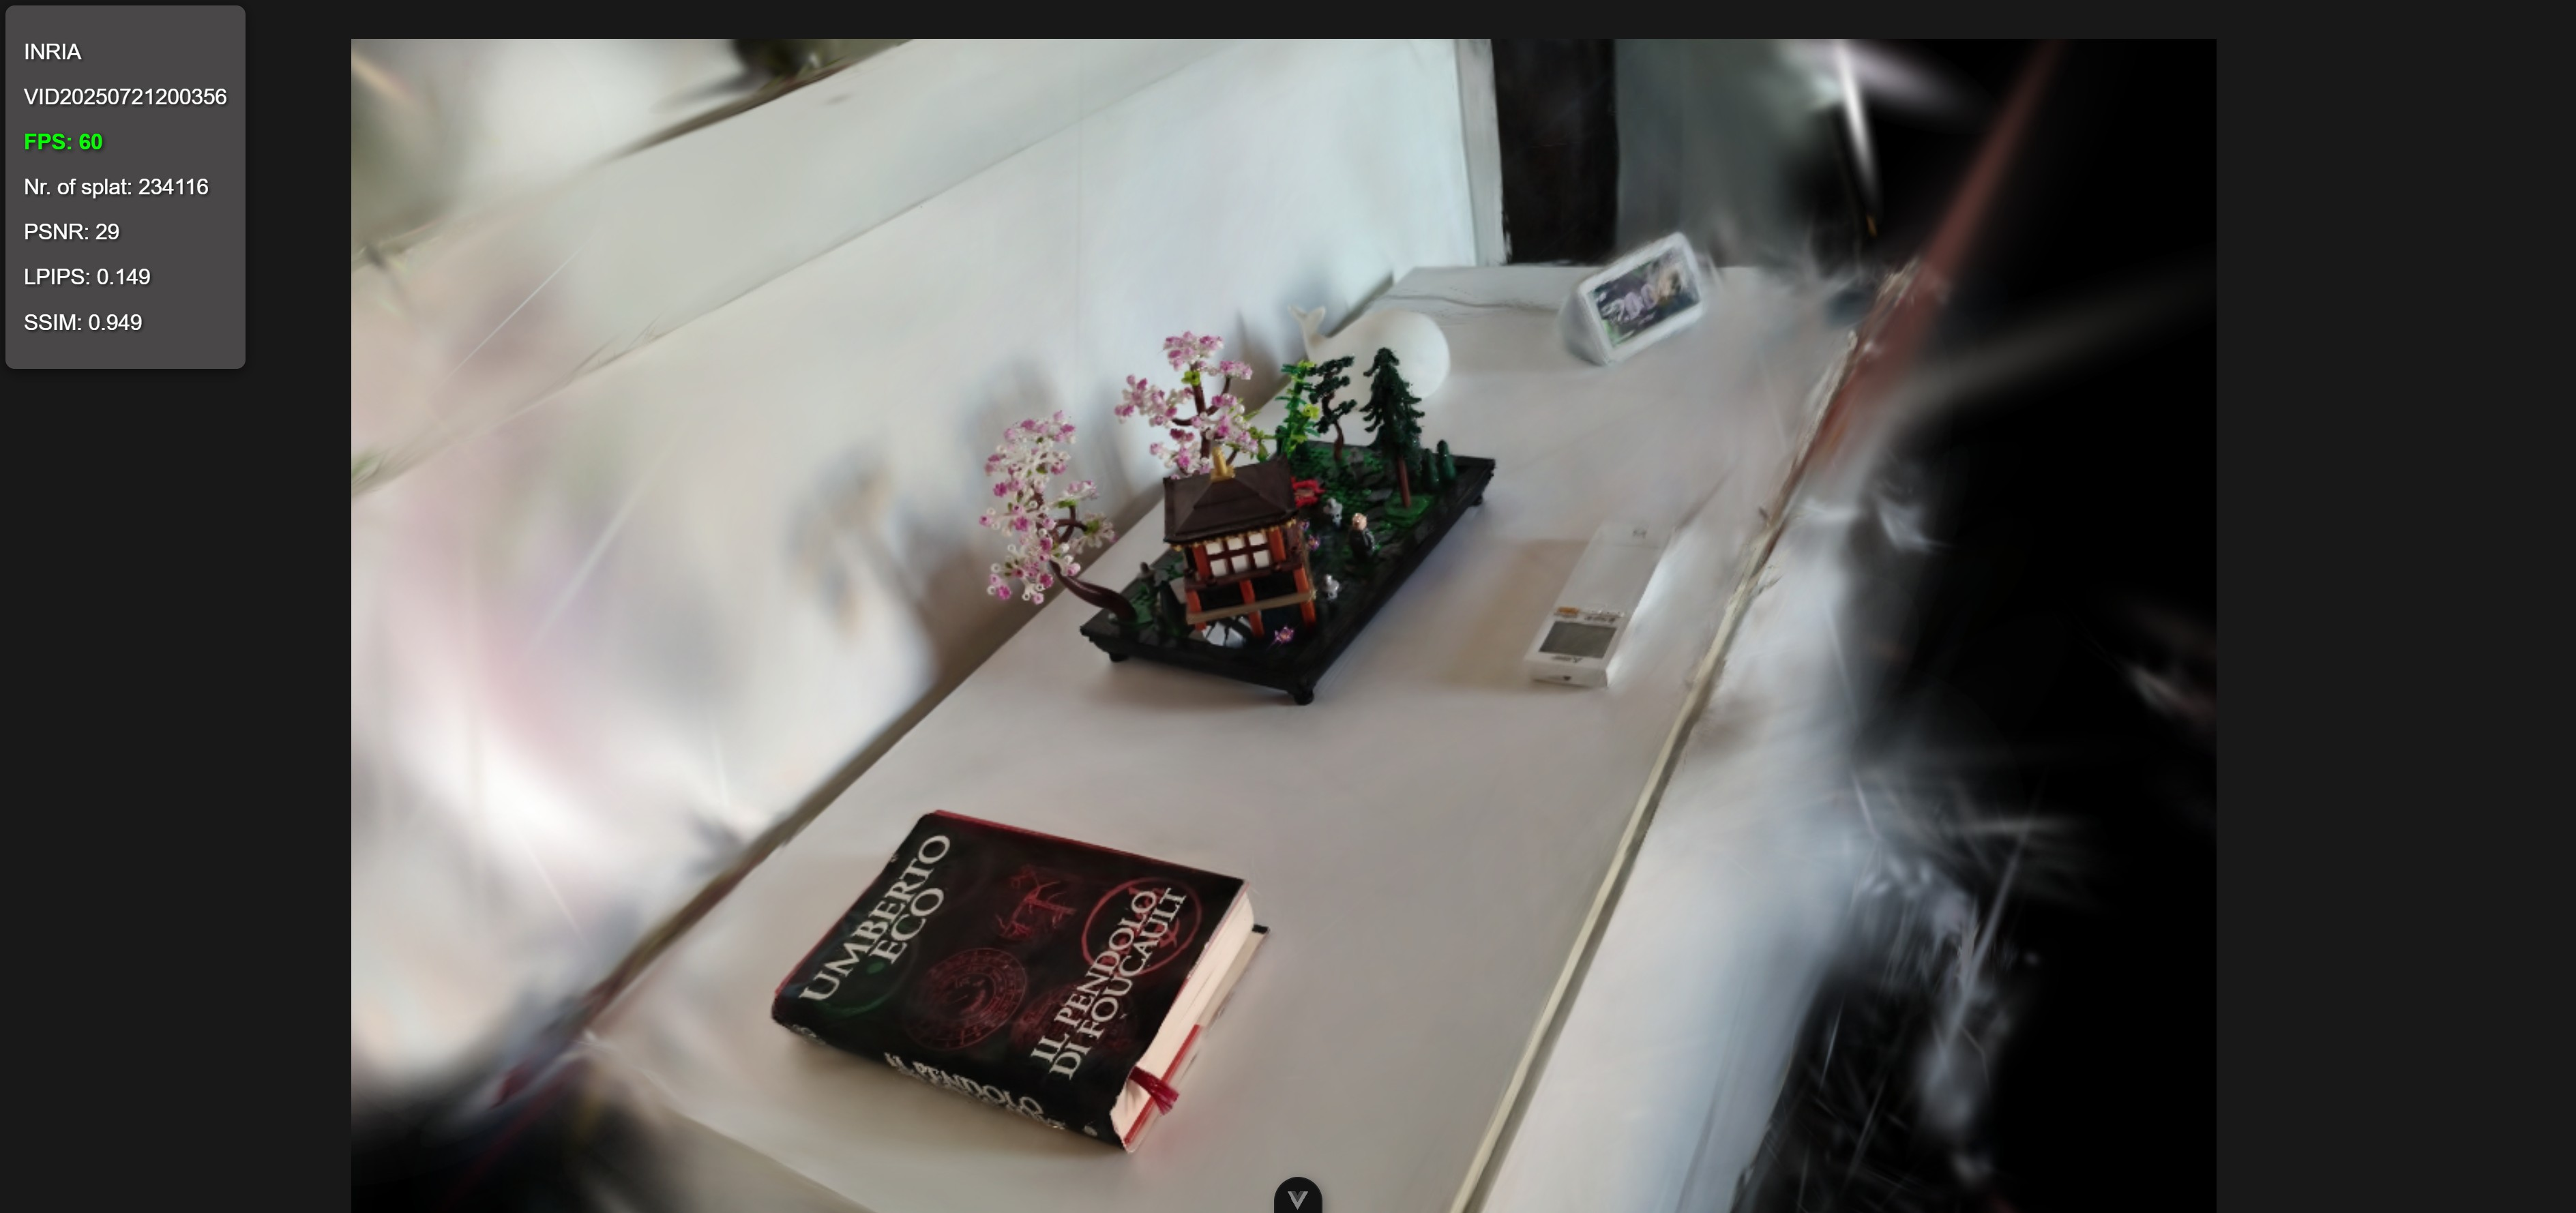
\includegraphics[width=\textwidth]{images/frontend_viewer_3.jpg}
	\caption{Visualizzazione di un modello complesso (Japanese garden) con rendering real-time a 60 FPS}
	\label{fig:viewer3d_complex}
\end{figure}
\newpage
\subsection{Ottimizzazione performance e UX}

Il frontend implementa diverse strategie per garantire un'esperienza utente fluida anche con dataset di grandi dimensioni:

\paragraph{Lazy Loading}
Le thumbnail e i dati dei modelli vengono caricati progressivamente durante lo scroll, riducendo il tempo di caricamento iniziale della dashboard.

\paragraph{Caching intelligente}
I modelli 3D visualizzati recentemente vengono mantenuti in cache del browser, permettendo switching istantaneo tra modelli già caricati.

\paragraph{Responsive Design}
Layout adattivi garantiscono usabilità ottimale su dispositivi desktop, tablet e mobile, con breakpoint specificamente ottimizzati per i pattern di utilizzo tipici del sistema.

\subsection{Integrazione con il Backend}

Il frontend mantiene una separazione netta tra logica di presentazione e business logic attraverso l'utilizzo di \textbf{Pinia} per lo state management. Questo approccio centralizzato permette:

\begin{itemize}
	\item \textbf{Sincronizzazione automatica} tra componenti che visualizzano gli stessi dati
	\item \textbf{Gestione consistente degli errori} con retry automatici per operazioni di rete fallite
	\item \textbf{Persistenza locale} di preferenze utente e stati di navigazione
	\item \textbf{Ottimizzazione delle chiamate API} attraverso batching e deduplicazione delle richieste
\end{itemize}

Il sistema di autenticazione JWT è integrato trasparentemente, con refresh automatico dei token e redirect intelligenti che preservano il contesto di navigazione dell'utente durante le operazioni di login/logout.\newline\newline

L'architettura complessiva del frontend riflette l'obiettivo primario del progetto: rendere la tecnologia del 3D Gaussian Splatting accessibile attraverso un'interfaccia che nasconde la complessità tecnica sottostante, guidando l'utente attraverso workflow ottimizzati che bilanciano automaticamente qualità dei risultati e risorse computazionali disponibili.
\chapter{Analisi Sperimentale e Valutazione Prestazioni}
\label{chap:analisi_sperimentale}

\section{Metodologia di Testing}
\label{sec:metodologia_testing}

\subsection{Obiettivi della Valutazione Sperimentale}
\label{subsec:obiettivi_valutazione}

La valutazione sperimentale del sistema è stata strutturata per analizzare sia le prestazioni degli algoritmi di training implementati che l'efficacia dell'architettura distribuita proposta. Gli obiettivi principali dell'analisi includono:

\begin{itemize}
	\item \textbf{Confronto qualitativo degli algoritmi}: Valutazione delle prestazioni relative tra Standard 3DGS, MCMC 3DGS e Taming 3DGS attraverso metriche standardizzate
	\item \textbf{Analisi dell'impatto dei parametri di qualità}: Studio dell'effetto dei livelli Fast, Balanced e Quality sulla qualità finale e sui tempi di elaborazione
	\item \textbf{Valutazione dell'architettura distribuita}: Analisi delle prestazioni del workflow end-to-end e identificazione di colli di bottiglia
	\item \textbf{Caratterizzazione utilizzo risorse}: Monitoring dettagliato di VRAM, GPU utilization e performance termiche durante l'elaborazione
\end{itemize}

\subsection{Dataset Video e Caratteristiche di Input}
\label{subsec:dataset_video_input}

Per garantire una valutazione comprensiva del sistema, è stato definito un set strutturato di scene reali che copre diversi livelli di complessità geometrica, ambientale e di ripresa. \textbf{Tutti i video sono stati acquisiti in risoluzione 4K (3840×2160) a 30 fps tramite la fotocamera di uno smartphone gamma medio-alta, cercando di garantire la massima qualità del dataset di partenza}, prima delle successive fasi di preprocessing adattivo.

\subsubsection{Categorizzazione delle Scene Video}

\textbf{S1 - Scene Geometriche Semplici}
\begin{itemize}
	\item \textbf{Spring Rider} (360°, Outdoor): Forme geometriche elementari con colori uniformi
	\begin{itemize}
		\item Durata: 1 minuto e 10 secondi
		\item Dimensione file: 345.569 KB
	\end{itemize}
	
	\item \textbf{Lego Japanese Garden} (180°, Indoor): Oggetto con geometrie regolari ma dettagli architetturali
	\begin{itemize}
		\item Durata: 1 minuto e 38 secondi  
		\item Dimensione file: 607.327 KB
	\end{itemize}
\end{itemize}

\textbf{S2 - Scene Multi-Oggetto}
\begin{itemize}
	\item \textbf{Master of Puppets} (180°, Indoor): Collezione di peluche con occlusioni multiple
	\begin{itemize}
		\item Durata: 1 minuto e 34 secondi
		\item Dimensione file: 579.644 KB
	\end{itemize}
	
	\item \textbf{Multiple Objects} (180°, Indoor): Lego garden + oggetti accessori, occlusioni ridotte  
	\begin{itemize}
		\item Durata: 1 minuto e 21 secondi
		\item Dimensione file: 498.843 KB
	\end{itemize}
	
	\item \textbf{Wall Plants} (240°, Outdoor): Struttura + pianta, combinazione artificiale/naturale
	\begin{itemize}
		\item Durata: 1 minuto e 8 secondi
		\item Dimensione file: 421.296 KB
	\end{itemize}
\end{itemize}

\textbf{S3 - Scene ad Alta Complessità}
\begin{itemize}
	\item \textbf{Yellow Plant} (360°, Outdoor): Dettagli fini naturali, illuminazione variabile
	\begin{itemize}
		\item Durata: 1 minuto e 40 secondi
		\item Dimensione file: 566.772 KB
	\end{itemize}
	
	\item \textbf{Lego Display Window} (360°, Indoor): Oggetti multipli in spazio confinato
	\begin{itemize}
		\item Durata: 1 minuto e 18 secondi
		\item Dimensione file: 479.009 KB
	\end{itemize}
	
	\item \textbf{My Workstation} (180°, Indoor): Ambiente complesso (TV, PC, mobili)
	\begin{itemize}
		\item Durata: 1 minuto e 14 secondi
		\item Dimensione file: 457.335 KB
	\end{itemize}
\end{itemize}

\begin{table}[htbp]
	\centering
	\caption{Caratteristiche dei video del dataset utilizzato}
	\label{tab:video_dataset_caratteristiche}
	\begin{tabular}{|p{3cm}|c|c|c|c|p{2.5cm}|}
		\hline
		\textbf{Scena} & \textbf{Durata} & \textbf{Dimensione} & \textbf{Ambiente} & \textbf{Angolo} & \textbf{Tipologia} \\
		\hline
		Spring Rider & 00:01:10 & 345.569 KB & Outdoor & 360° & Oggetto Singolo \\
		Lego Japanese Garden & 00:01:38 & 607.327 KB & Indoor & 180° & Oggetto Singolo \\
		Master of Puppets & 00:01:34 & 579.644 KB & Indoor & 180° & Multi-Oggetto \\
		Multiple Objects & 00:01:21 & 498.843 KB & Indoor & 180° & Multi-Oggetto \\
		Wall Plants & 00:01:08 & 421.296 KB & Outdoor & 240° & Misto \\
		Yellow Plant & 00:01:40 & 566.772 KB & Outdoor & 360° & Naturale \\
		Lego Display Window & 00:01:18 & 479.009 KB & Indoor & 360° & Multi-Oggetto \\
		My Workstation & 00:01:14 & 457.335 KB & Indoor & 180° & Ambiente Complesso \\
		\hline
	\end{tabular}
\end{table}

\subsection{Pipeline di Preprocessing e Adattamento Hardware}
\label{subsec:pipeline_preprocessing}

Il sistema implementa una \textbf{pipeline di preprocessing adattiva} che trasforma i video 4K di input in dataset ottimizzati per il training, applicando scaling dinamico basato sui vincoli hardware e sui livelli di qualità selezionati.

\subsubsection{Depth Regularization per Algoritmo INRIA}

\label{subsubsec:depth_regularization}

Il sistema implementa automaticamente una fase di \textbf{depth regularization} esclusivamente per l'algoritmo INRIA (Standard 3DGS), utilizzando il modello Depth Anything V2 per generare depth maps di supporto al training.

\paragraph{Pipeline Depth Regularization}
\begin{enumerate}
	\item \textbf{Generazione Depth Maps}: Depth Anything V2 analizza ogni frame estratto generando mappe di profondità monocromatiche
	\item \textbf{Scaling Parametri}: Generazione automatica di \texttt{depth\_params.json} con scale factors specifici per la scena
	\item \textbf{Training Depth-Aware}: Integrazione dei vincoli geometrici nel processo di ottimizzazione gaussiana
\end{enumerate}

\paragraph{Motivazioni della Scelta Algoritmo-Specifica}
\begin{itemize}
	\item \textbf{INRIA necessita supporto geometrico}: L'algoritmo originale può beneficiare di prior geometrici per scene complesse
	\item \textbf{MCMC e Taming sono auto-sufficienti}: Questi algoritmi incorporano meccanismi interni di regolarizzazione spaziale
	\item \textbf{Bilanciamento computazionale}: Evitare overhead inutile per algoritmi già ottimizzati
\end{itemize}

\begin{tcolorbox}[colback=orange!10,colframe=orange!50,title=Importante: Variabile Confondente nei Confronti]
	La depth regularization introduce una \textbf{variabile confondente} nei confronti diretti tra algoritmi. I risultati INRIA nei benchmark includeranno sempre depth regularization, rendendo i confronti non perfettamente equi. Questo riflette tuttavia l'utilizzo ottimale di ciascun algoritmo nelle condizioni reali di deployment.
\end{tcolorbox}

\subsubsection{Post-Processing: Conversione PLY→KSPLAT e Variante Taming}

Il sistema implementa la \textbf{conversione PLY→KSPLAT} per tutti gli algoritmi di training. Tutti gli algoritmi generano output in formato PLY standard, che viene convertito nel formato KSPLAT per ottenere file significativamente più compatti e ottimizzati per la visualizzazione web.

\textbf{Variante Specifica Taming}: Durante la conversione standard PLY→KSPLAT, l'algoritmo Taming richiede un'ulteriore trasformazione dei valori di opacity. Taming genera valori di opacity in formato sigmoid che necessitano di conversione per compatibilità ottimale con i viewer 3D.

\textbf{Trasformazione Implementata}: Per l'output Taming, viene applicata automaticamente una trasformazione inverse sigmoid (logit) durante la fase di conversione:
\begin{lstlisting}[language=Python, caption=Conversione opacity per Taming]
	logit_opacity = log(opacity / (1.0 - opacity))
\end{lstlisting}

Questa sotto-conversione ha impatto computazionale trascurabile ed è trasparente all'utente, garantendo formato uniforme e interoperabilità con tutti i viewer utilizzati.
\subsection{Ambiente di Deployment e Configurazione Hardware}
\label{subsec:ambiente_deployment}

\subsubsection{Setup Hardware di Test}

I test sono stati eseguiti su configurazione hardware che riflette un ambiente di deployment medio piuttosto che una configurazione ideale da laboratorio:

\paragraph{Configurazione GPU}
\begin{itemize}
	\item \textbf{GPU}: NVIDIA GeForce RTX 4080
	\item \textbf{VRAM Disponibile}: 16 GB -- \textbf{Significativamente inferiore} ai 24GB raccomandati nella documentazione del 3D Gaussian Splatting originale
	\item \textbf{Architettura}: CUDA Compute Capability 8.9 per Ada Lovelace
\end{itemize}

\paragraph{Sistema Host}
\begin{itemize}
	\item \textbf{OS}: Windows 11 Pro
	\item \textbf{Ambiente}: WSL2 (Windows Subsystem for Linux) con Ubuntu 22.04
	\item \textbf{Container Runtime}: Docker Desktop con Docker Compose
	\item \textbf{CPU}: AMD 7800X3D 4.2Ghz 96 Mo L3 
	\item \textbf{RAM Sistema}: 32 GB DDR5 limitati a 20 GB per i container con memory swapping a 32 GB
	\item \textbf{Storage}: SSD NVMe per minimizzare latenze I/O
\end{itemize}

\subsubsection{Sistema di Monitoring Hardware Real-Time}
\label{subsubsec:monitoring_hardware}

Per caratterizzare accuratamente il comportamento degli algoritmi sotto vincoli hardware, è stato implementato un \textbf{monitoring system} che raccoglie metriche GPU durante l'intero ciclo di training.

\paragraph{Metriche Hardware Monitorate}
\begin{lstlisting}[language=JavaScript, caption=Esempio statistiche hardware raccolte]
	{
		"peak_vram_mb": 14535,        // Picco utilizzo VRAM
		"avg_vram_mb": 12106.3,       // Utilizzo medio VRAM
		"min_vram_mb": 2242,          // Baseline VRAM (modello + overhead)
		"avg_gpu_utilization": 90,    // Utilizzo GPU medio (%)
		"max_temperature_c": 79,      // Temperatura massima raggiunta
		"monitoring_duration_s": 1362.4, // Durata totale training
		"total_samples": 449          // Campioni raccolti (ogni 3s)
	}
\end{lstlisting}

\paragraph{Implementazione Tecnica}
\begin{itemize}
	\item \textbf{Sampling Rate}: 3 secondi per bilanciare granularità e overhead
	\item \textbf{Host-Level Monitoring}: Raccolta diretta da GPU driver, indipendente dai container
	\item \textbf{Persistenza Automatica}: Integrazione nei metadati del workflow per analisi retrospettive
\end{itemize}

\subsection{Metodologia di Valutazione}
\label{subsec:metodologia_valutazione}

\subsubsection{Metriche Quantitative Automatizzate}

Il sistema implementa automaticamente il calcolo delle tre metriche standard per la valutazione della qualità di rendering:

\begin{itemize} 
	\item \textbf{PSNR (Peak Signal-to-Noise Ratio)}
\begin{itemize}
	\item Range tipico: 20--40 dB
	\item Valori superiori indicano minore rumore e maggiore fedelt\`a
	\item \textit{Osservazione}: valori \textgreater 25 dB sono considerati buoni, ma soglie pi\`u basse (22--24 dB) possono comunque essere accettabili in contesti reali e con hardware limitato
\end{itemize}

\item \textbf{SSIM (Structural Similarity Index)}
\begin{itemize}
	\item Range: 0--1
	\item Valori elevati indicano maggiore similarit\`a strutturale
	\item Soglia di accettabilit\`a: \textgreater 0.8 (con valori tra 0.75 e 0.8 ancora ritenuti adeguati)
\end{itemize}

\item \textbf{LPIPS (Learned Perceptual Image Patch Similarity)}
\begin{itemize}
	\item Range: 0--1 (valori inferiori indicano maggiore similarit\`a percettiva)
	\item Obiettivo qualitativo: \textless 0.2 in condizioni ideali
	\item \textit{Nota}: valori fino a 0.25 possono essere ritenuti accettabili per scene complesse o condizioni hardware non ottimali
\end{itemize}
\end{itemize}
\section{Benchmark e Risultati Sperimentali}
\label{sec:benchmark_risultati}

\subsection{Benchmark 1: Confronto Algoritmi e Scalabilità Hardware}
\label{subsec:benchmark1_sintetico}

Il primo benchmark ha l’obiettivo di confrontare le tre varianti di 3D Gaussian Splatting considerate in questa tesi — INRIA (implementazione standard con \textit{depth regularization}), MCMC 3DGS e Taming 3DGS — valutandone prestazioni, scalabilità e qualità visiva. 
Il test è stato condotto su tre scene di riferimento: \textbf{S1} \textit{Spring Rider}, caratterizzata da geometria semplice e ripresa a 360° in ambiente outdoor; \textbf{S2} \textit{Tomatoes}, con dettagli organici fini, ideale per analizzare l’impatto dell’aumento di risoluzione; e \textbf{S3} \textit{My Workstation}, una scena indoor complessa con oggetti multipli.

L’analisi mira a:
\begin{itemize}
	\item identificare punti di forza e debolezza di ciascun approccio;
	\item misurare la qualità di rendering mediante metriche quantitative (PSNR, SSIM, LPIPS);
	\item verificare la stabilità termica e l’utilizzo di VRAM in scenari reali;
	\item valutare la scalabilità con l’aumento della risoluzione fino al \textit{breaking point}.
\end{itemize}

Le sottosezioni seguenti presentano:
\begin{enumerate}
	\item una \textbf{sintesi comparativa} per avere a colpo d’occhio le differenze principali;
	\item i \textbf{risultati quantitativi} sulle scene di test;
	\item un \textbf{confronto qualitativo visuale} supportato da esempi;
	\item \textbf{considerazioni operative} e raccomandazioni per l’uso.
\end{enumerate}


\paragraph{Algoritmi:} INRIA (3DGS standard + depth regularization), MCMC 3DGS, Taming 3DGS \\

\paragraph{Scene di test:} 
\begin{itemize}
	\item \textbf{S1} -- Spring Rider: geometria semplice, outdoor, 360°
	\item \textbf{S2} -- Tomatoes: dettagli organici fini, ideale per test di upscaling
	\item \textbf{S3} -- My Workstation: indoor complesso, oggetti multipli
\end{itemize}

% ---------------------------------------------------
\subsubsection*{1. Sintesi comparativa}


\begin{table}[H]
	\centering
	\caption{Sintesi comparativa algoritmi}
	\label{tab:benchmark1_exec_summary}
	\begin{threeparttable}
		\setlength{\tabcolsep}{7pt}           % spaziatura colonne
		\renewcommand{\arraystretch}{1.15}    % altezza righe
		
		% NOTA: uso 0.95\linewidth per evitare che stringa "Taming" vada a capo
		\begin{tabularx}{0.95\linewidth}{l *{3}{>{\centering\arraybackslash}X}}
			\toprule
			\textbf{Criterio} & \textbf{INRIA} & \textbf{MCMC} & \textbf{\mbox{Taming}} \\
			\midrule
			Qualità media           & \warn & \cmark & \cmark \\
			Velocità                & \cmark & \xmark & \cmark \\
			Scalabilità risoluzione & \xmark & \warn  & \warn \\
			Stabilità termica       & \warn  & \cmark & \cmark \\
			Predicibilità VRAM      & \xmark & \warn  & \warn \\
			Artefatti               & \warn  & \xmark & \cmark \\
			\bottomrule
		\end{tabularx}
		
		\vspace{0.35em}
		\begin{minipage}{0.95\linewidth}
			\centering\footnotesize
			\textbf{Legenda:} \cmark\;=\;punto di forza,\quad
			\warn\;=\;adeguato,\quad
			\xmark\;=\;debolezza.
		\end{minipage}
	\end{threeparttable}
\end{table}

% ---------------------------------------------------
\subsubsection*{2. Risultati quantitativi}

\paragraph{Metriche medie (S1 + S3, profilo \textit{Balanced})}
\begin{table}[H]
	\centering
	\caption{Metriche medie su scene rappresentative}
	\label{tab:benchmark1_metrics_avg}
	\begin{tabularx}{0.9\linewidth}{l Y Y Y Y Y Y}
		\toprule
		\textbf{Algoritmo} & \textbf{PSNR↑} & \textbf{SSIM↑} & \textbf{LPIPS↓} & \textbf{Tempo} & \textbf{Peak VRAM} & \textbf{Temp max} \\
		\midrule
		INRIA* & 23.4 & 0.835 & 0.209 & 23m & 12.7 GB & 77.5°C \\
		MCMC   & 27.6 & 0.909 & 0.151 & 42m & 13.6 GB & 70.5°C \\
		Taming & 28.3 & 0.922 & \textbf{0.132} & \textbf{20m} & 13.8 GB & \textbf{69°C} \\
		\bottomrule
	\end{tabularx}
\end{table}

\paragraph{Qualità alla massima risoluzione stabile (S2)}
MCMC e Taming raggiungono 1080p nella maggior parte dei casi, ma possono manifestare degrado prestazionale o crash per spike di VRAM. INRIA si ferma stabilmente a 720p.

\begin{table}[H]
	\centering
	\caption{Qualità alla massima risoluzione stabile}
	\label{tab:benchmark1_resolution_quality}
	\begin{tabularx}{0.8\linewidth}{l >{\centering\arraybackslash}X >{\centering\arraybackslash}X >{\centering\arraybackslash}X >{\centering\arraybackslash}X}
		\toprule
		\textbf{Algoritmo} & \textbf{Res Max} & \textbf{PSNR} & \textbf{SSIM} & \textbf{LPIPS} \\
		\midrule
		INRIA* & 720p  & 21.5 & 0.724 & 0.249 \\
		MCMC   & 1080p & 23.9 & 0.751 & 0.247 \\
		Taming & 1080p & 24.0 & 0.752 & 0.248 \\
		\bottomrule
	\end{tabularx}
\end{table}

\paragraph{Andamento utilizzo VRAM per risoluzione}
L’analisi dell’andamento temporale dell’utilizzo di memoria video evidenzia differenze significative tra algoritmi e risoluzioni.
I punti contrassegnati come \textbf{OOM} indicano un arresto o degrado grave dovuto al superamento del limite di VRAM disponibile.

% Preambolo (assicurati di avere già)
% \usepackage{pgfplots}
% \usepackage{pgfplotstable}
% \pgfplotsset{compat=1.18}
% \usepgfplotslibrary{groupplots}
% \definecolor{inriacol}{RGB}{60,60,60}
% \definecolor{mcmccol}{RGB}{200,40,40}
% \definecolor{tamingcol}{RGB}{20,140,70}

\begin{figure}[H]
	\centering
	\begin{tikzpicture}
		\begin{groupplot}[
			group style={group size=2 by 2, horizontal sep=1.2cm, vertical sep=3.0cm},
			width=0.45\linewidth, height=5.3cm,
			grid=both, grid style={opacity=0.15},
			xlabel={Tempo [s]}, ylabel={VRAM [GB]},
			tick style={black}, tick label style={/pgf/number format/fixed},
			legend style={nodes={scale=0.95, transform shape}},
			legend to name=leg:vram
			]
			
			% -------- 480p --------
			\nextgroupplot[title={480p}]
			\addplot+[very thick, no marks, color=inriacol]   table[x index=0,y index=1,col sep=comma]{docs/480inria.csv};  \addlegendentry{INRIA}
			\addplot+[very thick, no marks, color=mcmccol]    table[x index=0,y index=1,col sep=comma]{docs/480mcmc.csv};   \addlegendentry{MCMC}
			\addplot+[very thick, no marks, color=tamingcol]  table[x index=0,y index=1,col sep=comma]{docs/480taming.csv};
			
			% -------- 720p --------
			\nextgroupplot[title={720p}]
			\addplot+[very thick, no marks, color=inriacol]   table[x index=0,y index=1,col sep=comma]{docs/720inria.csv};
			\addplot+[very thick, no marks, color=mcmccol]    table[x index=0,y index=1,col sep=comma]{docs/720mcmc.csv};
			\addplot+[very thick, no marks, color=tamingcol]  table[x index=0,y index=1,col sep=comma]{docs/720taming.csv};
			
			% -------- 1080p --------
			\nextgroupplot[title={1080p}]
			\addplot+[very thick, no marks, color=inriacol]   table[x index=0,y index=1,col sep=comma]{docs/1080inria.csv};
			\addplot+[very thick, no marks, color=mcmccol]    table[x index=0,y index=1,col sep=comma]{docs/1080mcmc.csv};
			\addplot+[very thick, no marks, color=tamingcol]  table[x index=0,y index=1,col sep=comma]{docs/1080taming.csv};
			% Marker OOM INRIA 1080p
			\addplot[only marks, mark=*, mark options={fill=white,draw=red}, red]
			table[x=x, y=y, col sep=comma]{docs/oom_1080_inria.csv};
			
			% -------- 1440p --------
			\nextgroupplot[title={1440p}]
			\addplot+[very thick, no marks, color=inriacol]   table[x index=0,y index=1,col sep=comma]{docs/1440inria.csv};
			\addplot+[very thick, no marks, color=mcmccol]    table[x index=0,y index=1,col sep=comma]{docs/1440mcmc.csv};
			\addplot+[very thick, no marks, color=tamingcol]  table[x index=0,y index=1,col sep=comma]{docs/1440taming.csv};
			% Marker OOM tutti algoritmi 1440p
			\addplot[only marks, mark=*, mark options={fill=white,draw=red}, red]
			table[x=x, y=y, col sep=comma]{docs/oom_1440_all.csv};
			
		\end{groupplot}
	\end{tikzpicture}
	
	\vspace{0.3em}
	\small\ref{leg:vram}
	
	\caption{Profilo di utilizzo VRAM nel tempo su \textbf{S2 Tomatoes}, per risoluzioni crescenti e algoritmi (INRIA/MCMC/Taming).
		I marker rossi indicano spike di VRAM associati a degrado prestazionale o arresto del training (non sempre OOM “hard”).}
	\label{fig:tomatoes_vram_profiles}
\end{figure}
  

% ---------------------------------------------------
\subsubsection*{3. Confronto qualitativo visuale}


\begin{figure}[ht]
	\centering
	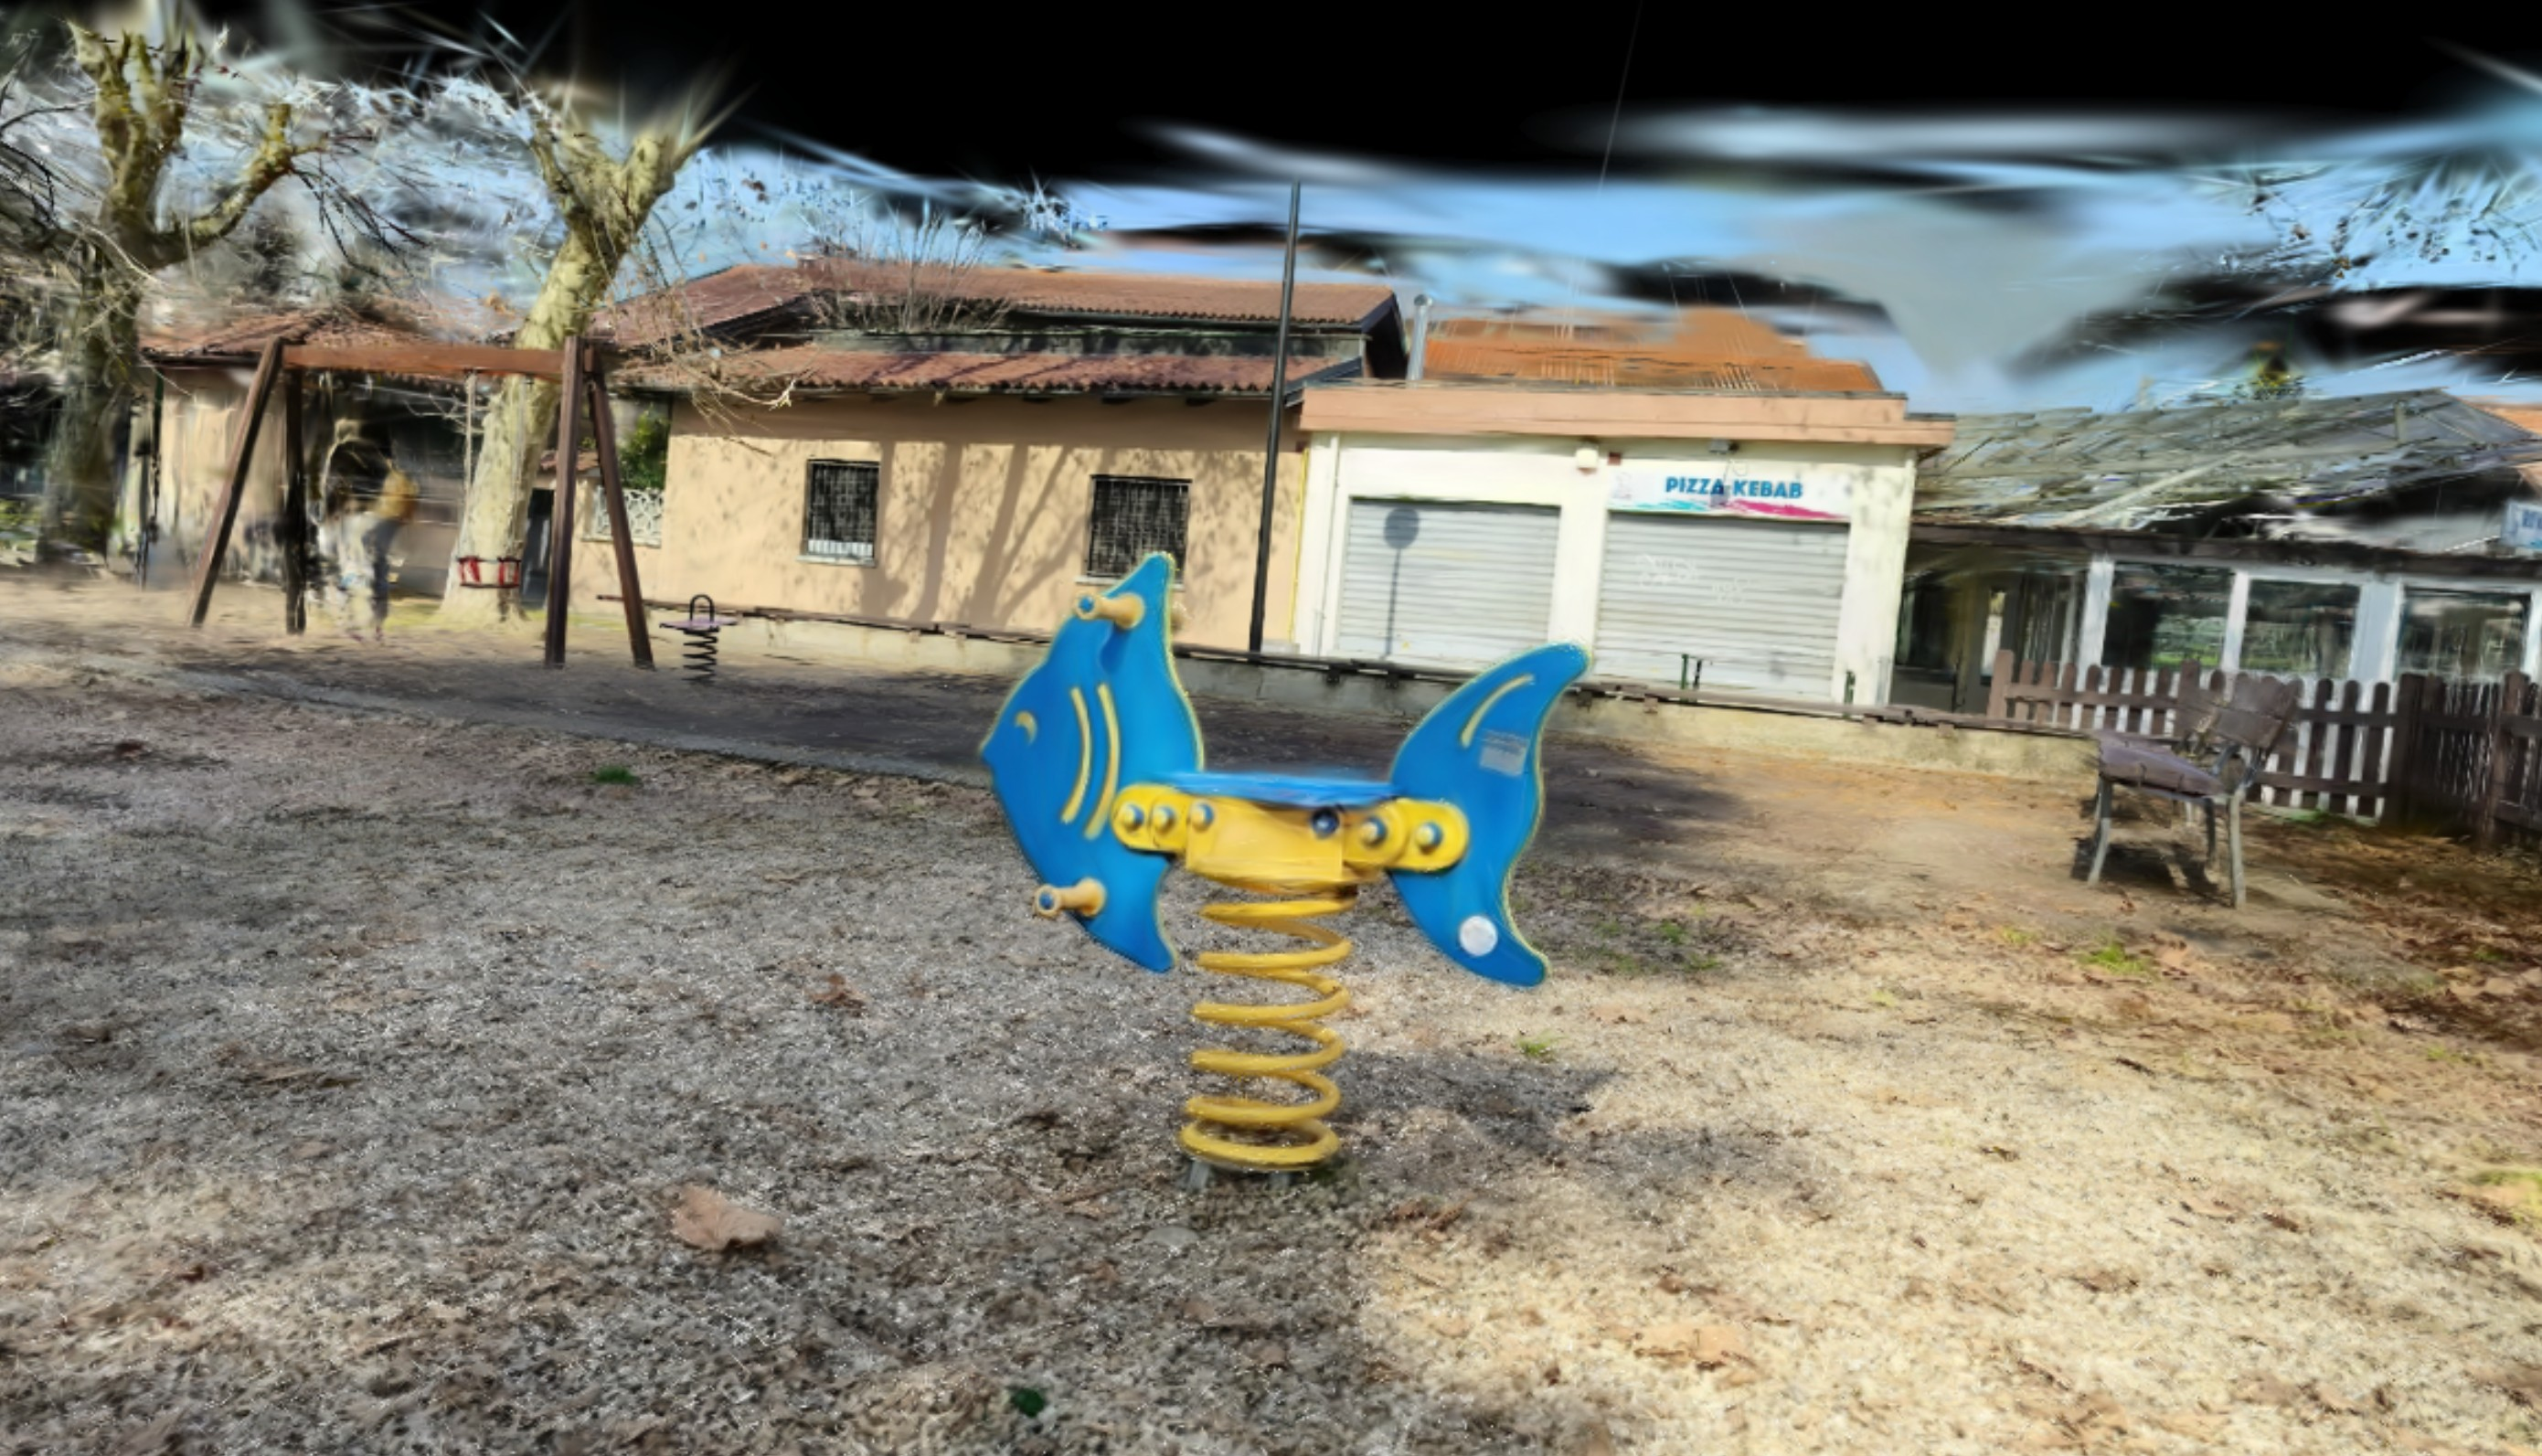
\includegraphics[width=0.32\textwidth,height=2.8cm,trim={80 40 80 40},clip]{images/benchmarks/spring_rider_inria_balanced_1.jpg}
	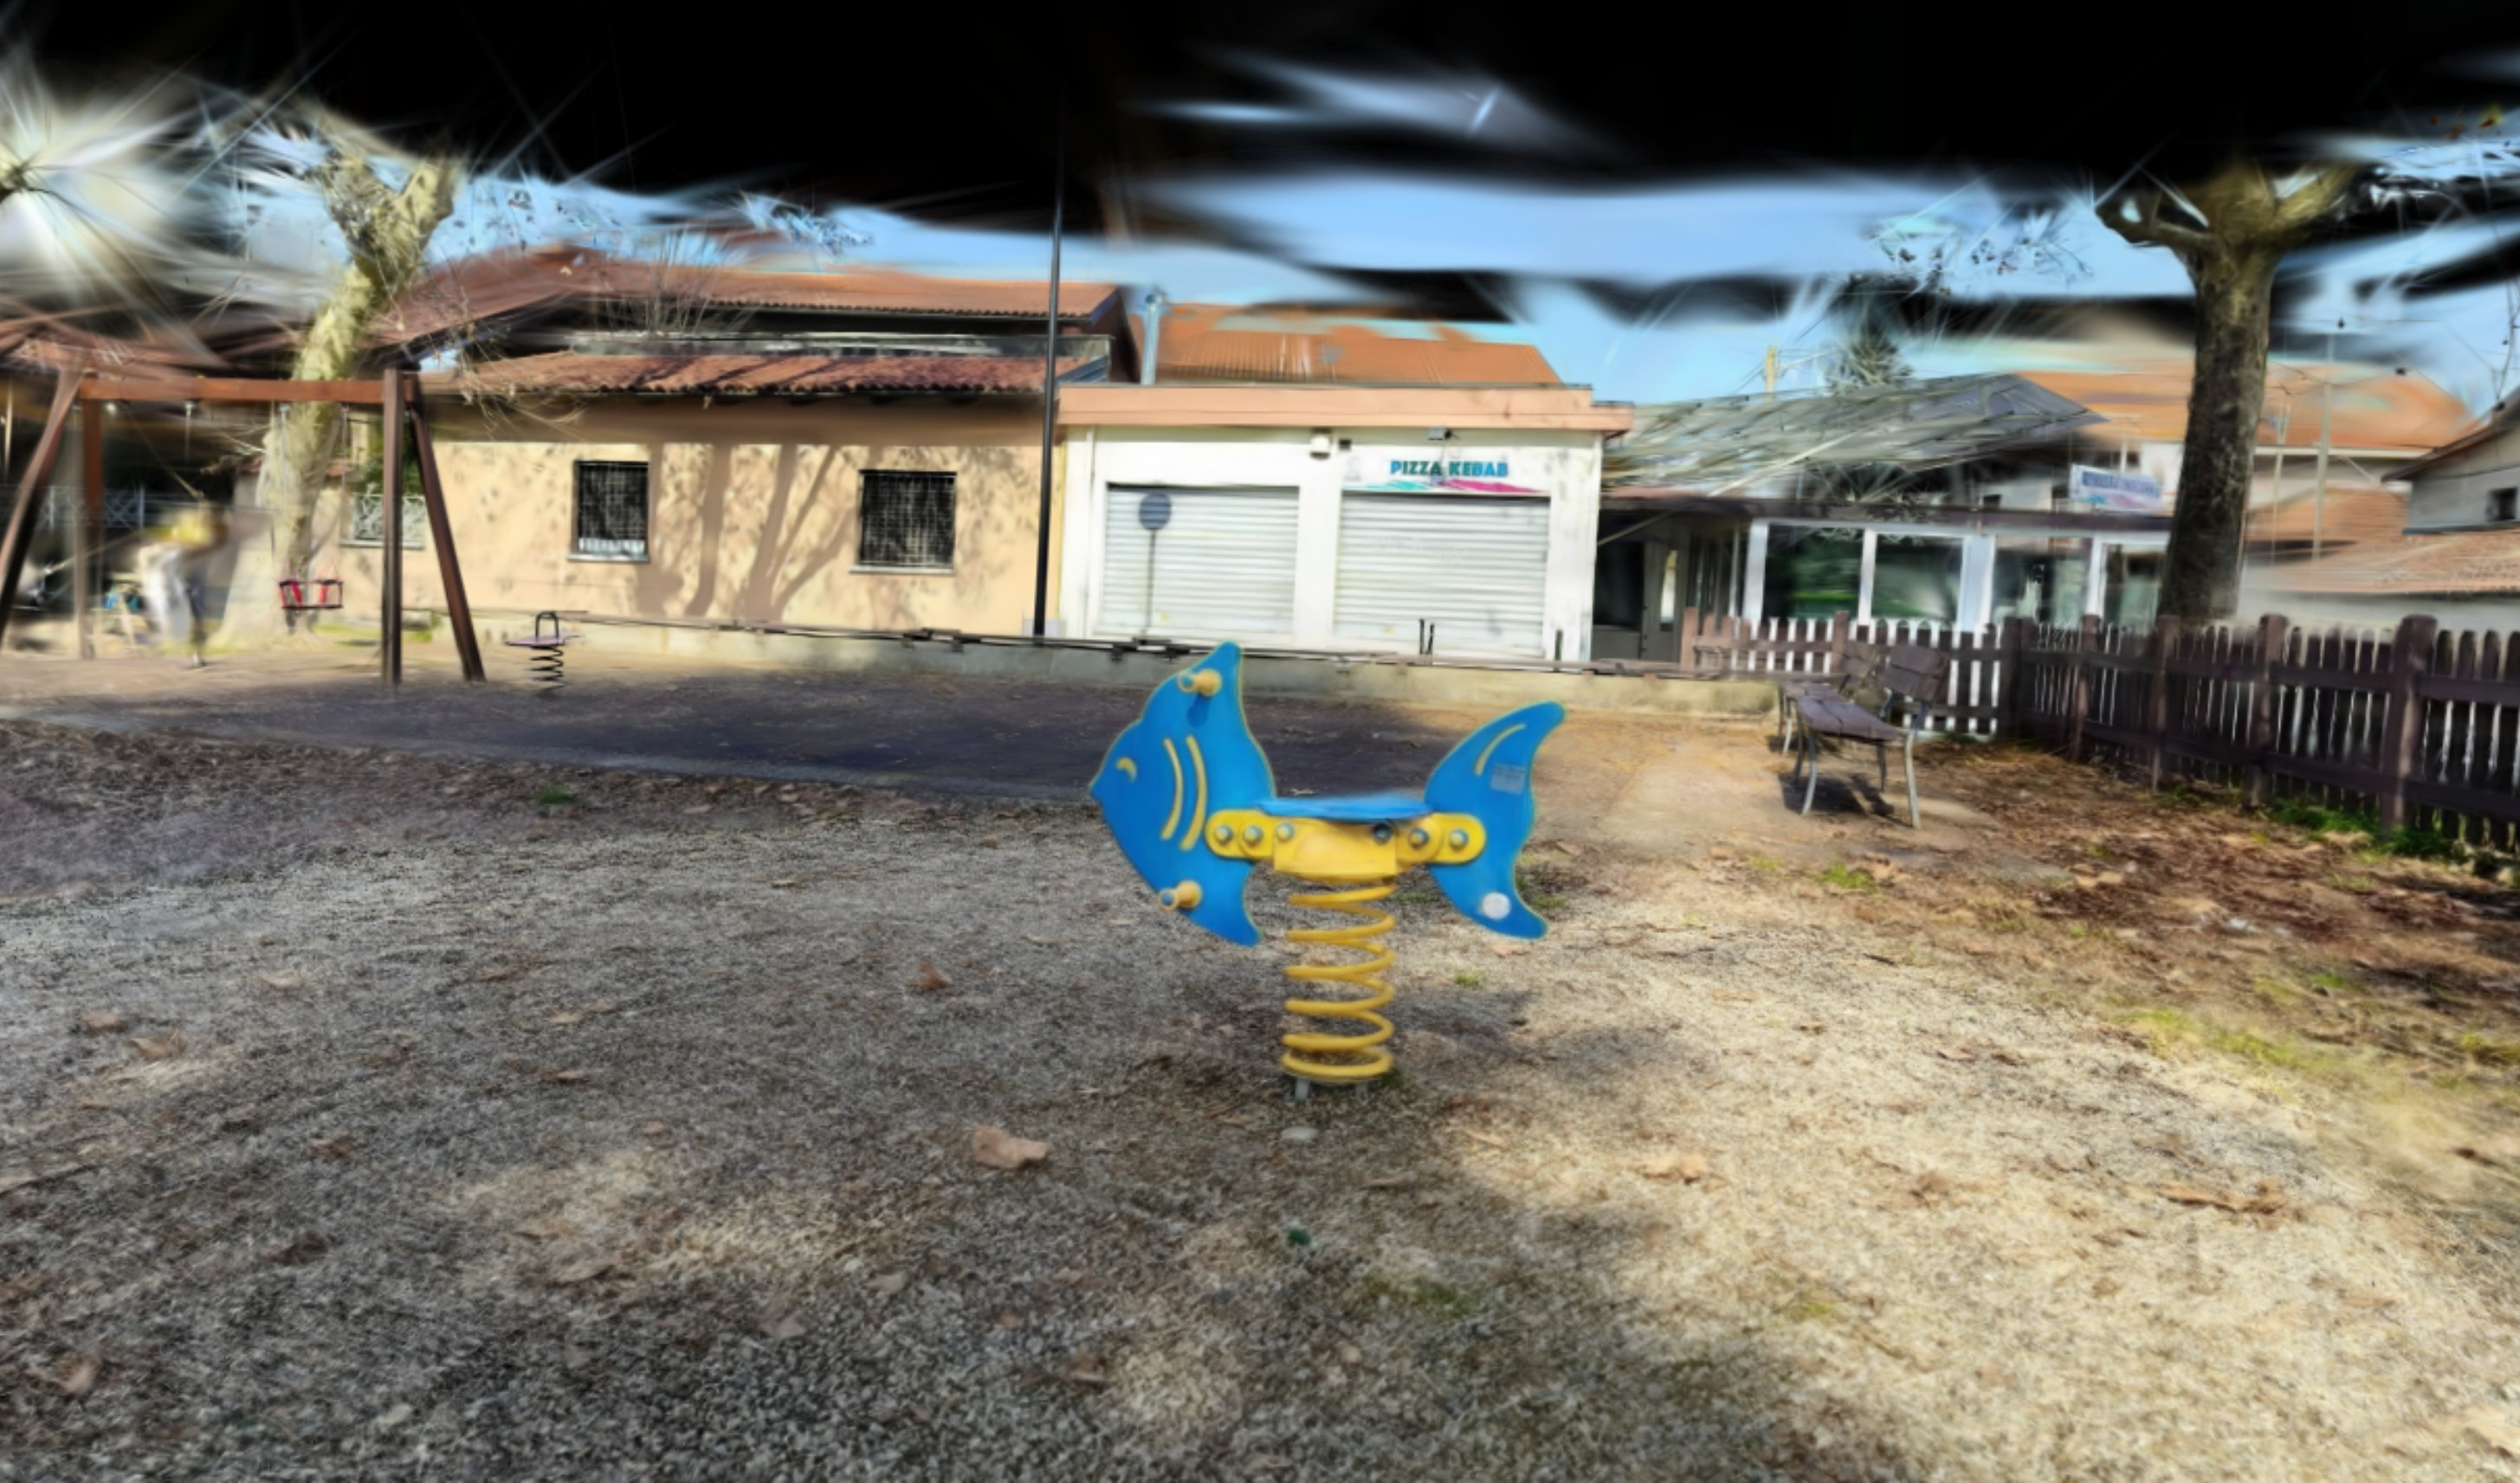
\includegraphics[width=0.32\textwidth,height=2.8cm,trim={80 40 80 40},clip]{images/benchmarks/spring_rider_mcmc_balanced_1.jpg}
	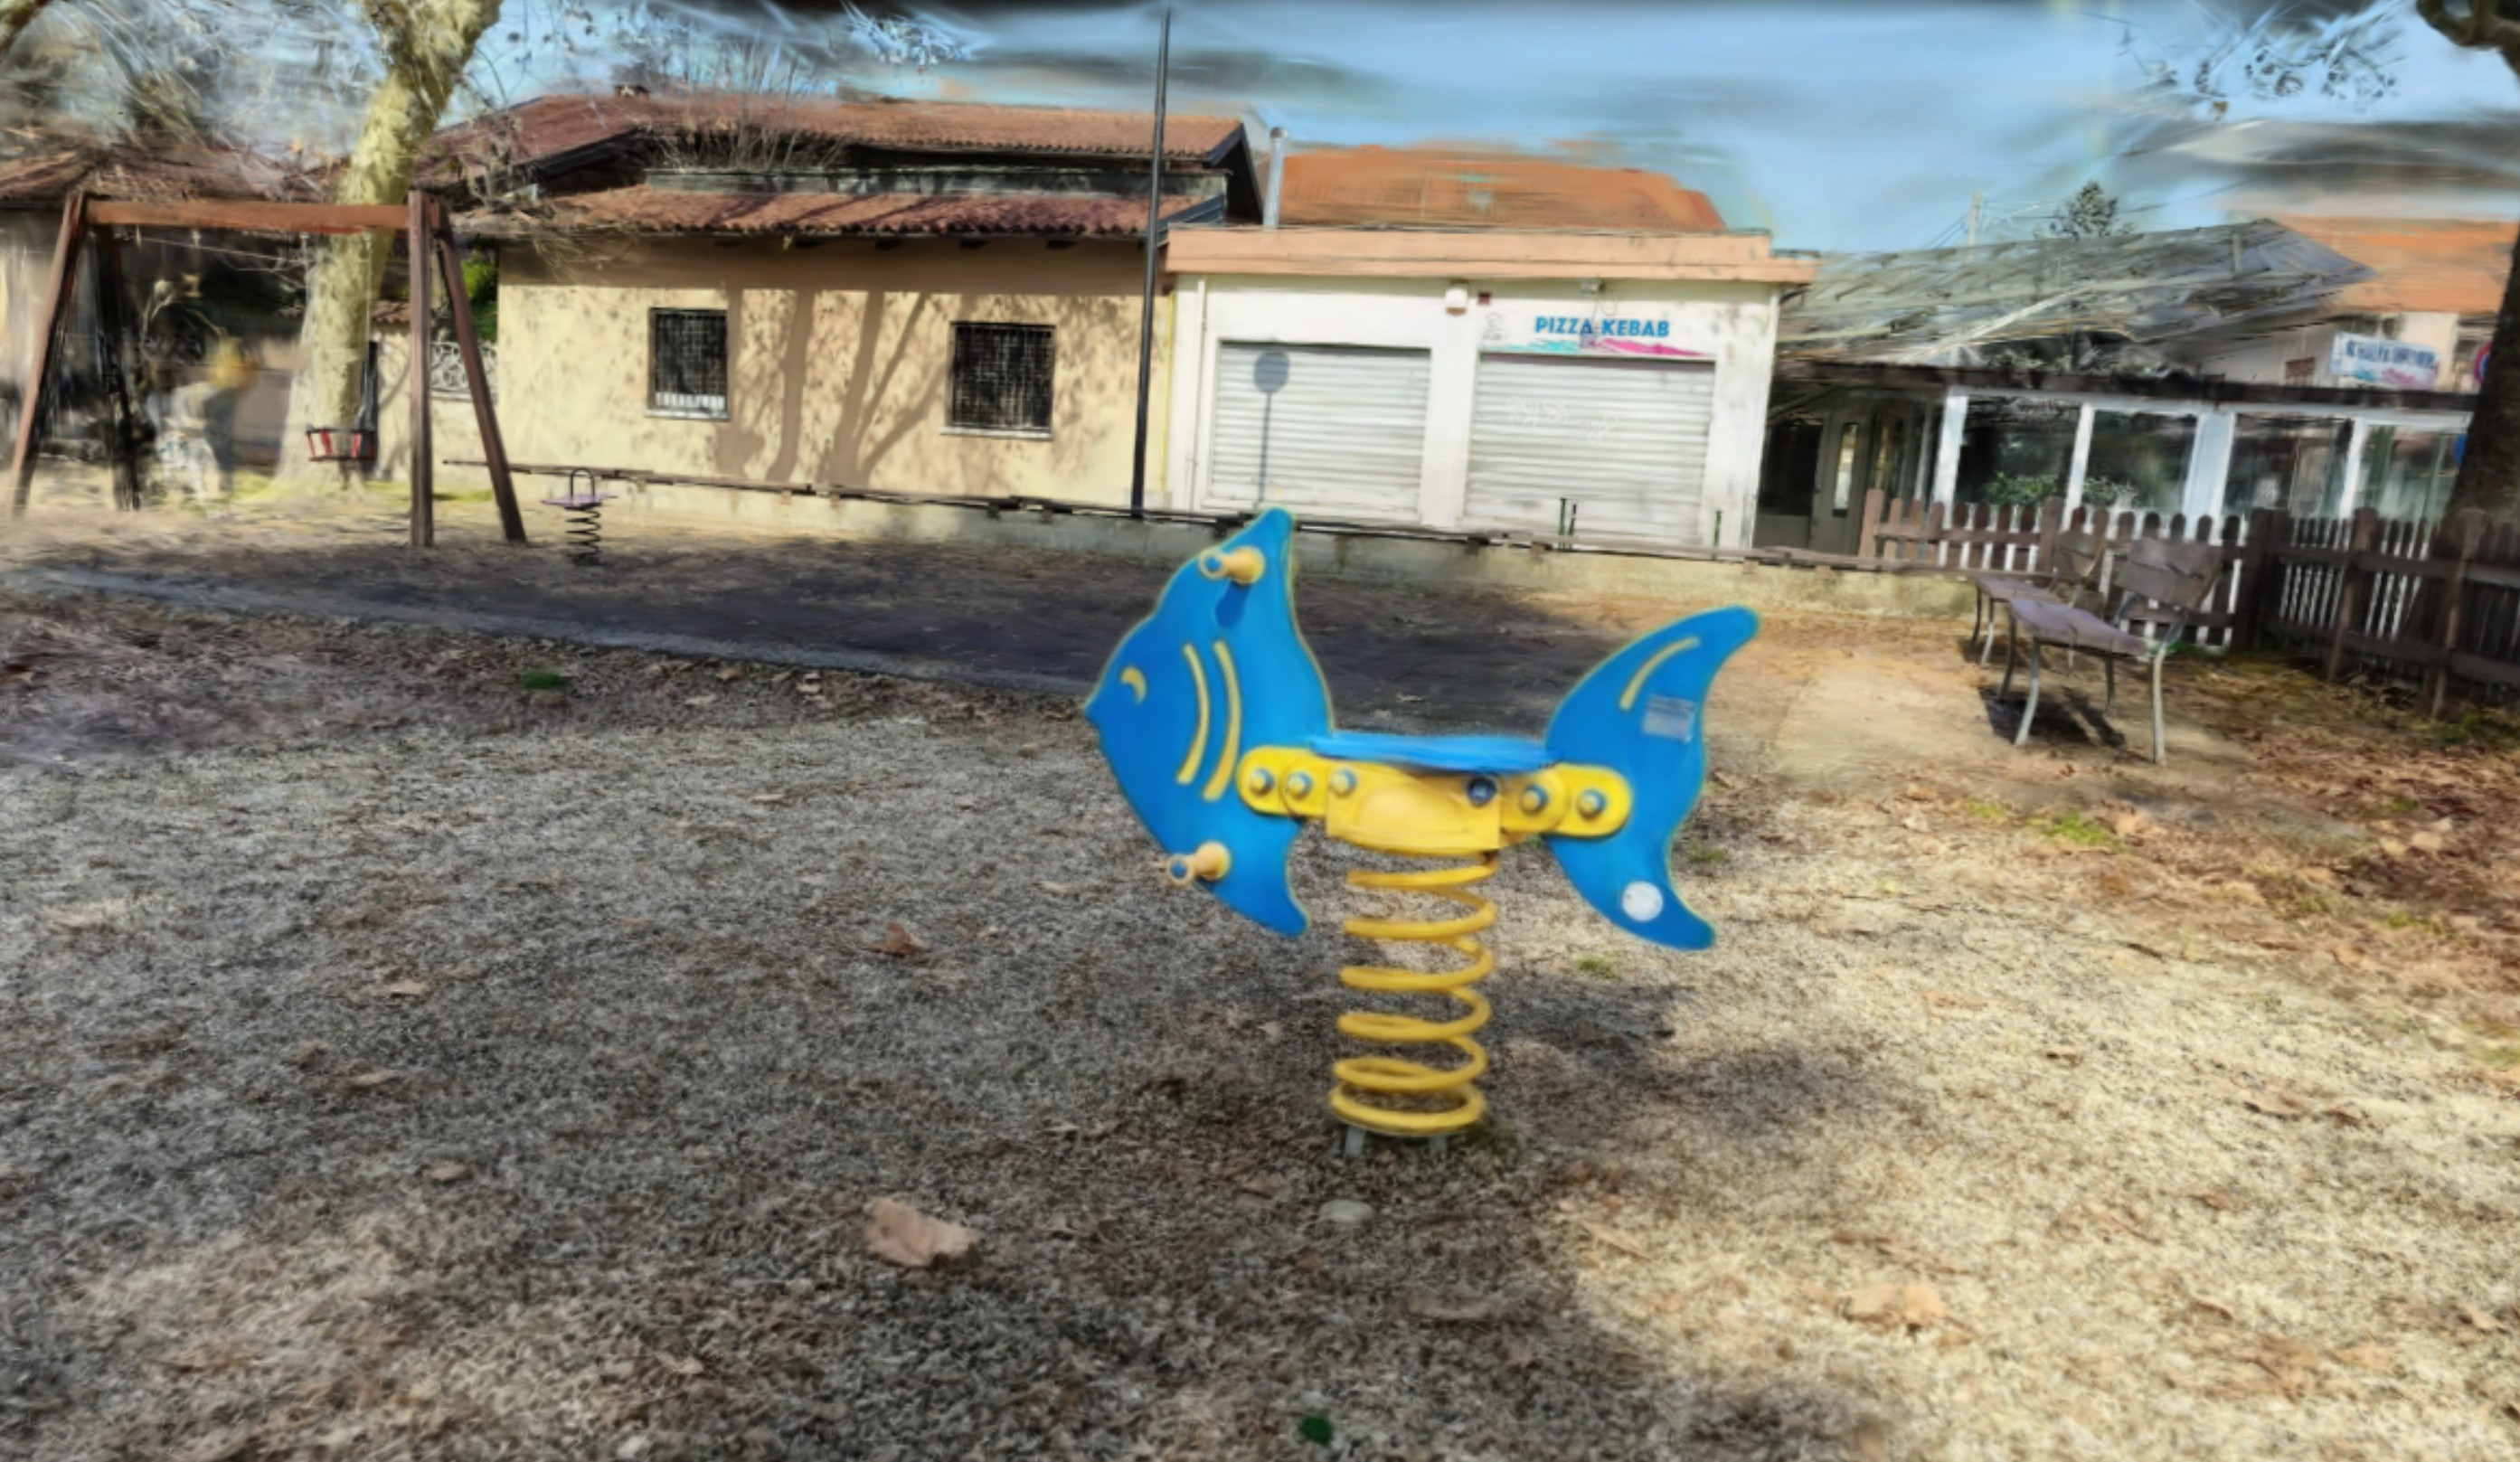
\includegraphics[width=0.32\textwidth,height=2.8cm,trim={80 40 80 40},clip]{images/benchmarks/spring_rider_taming_balanced_1.jpg}
	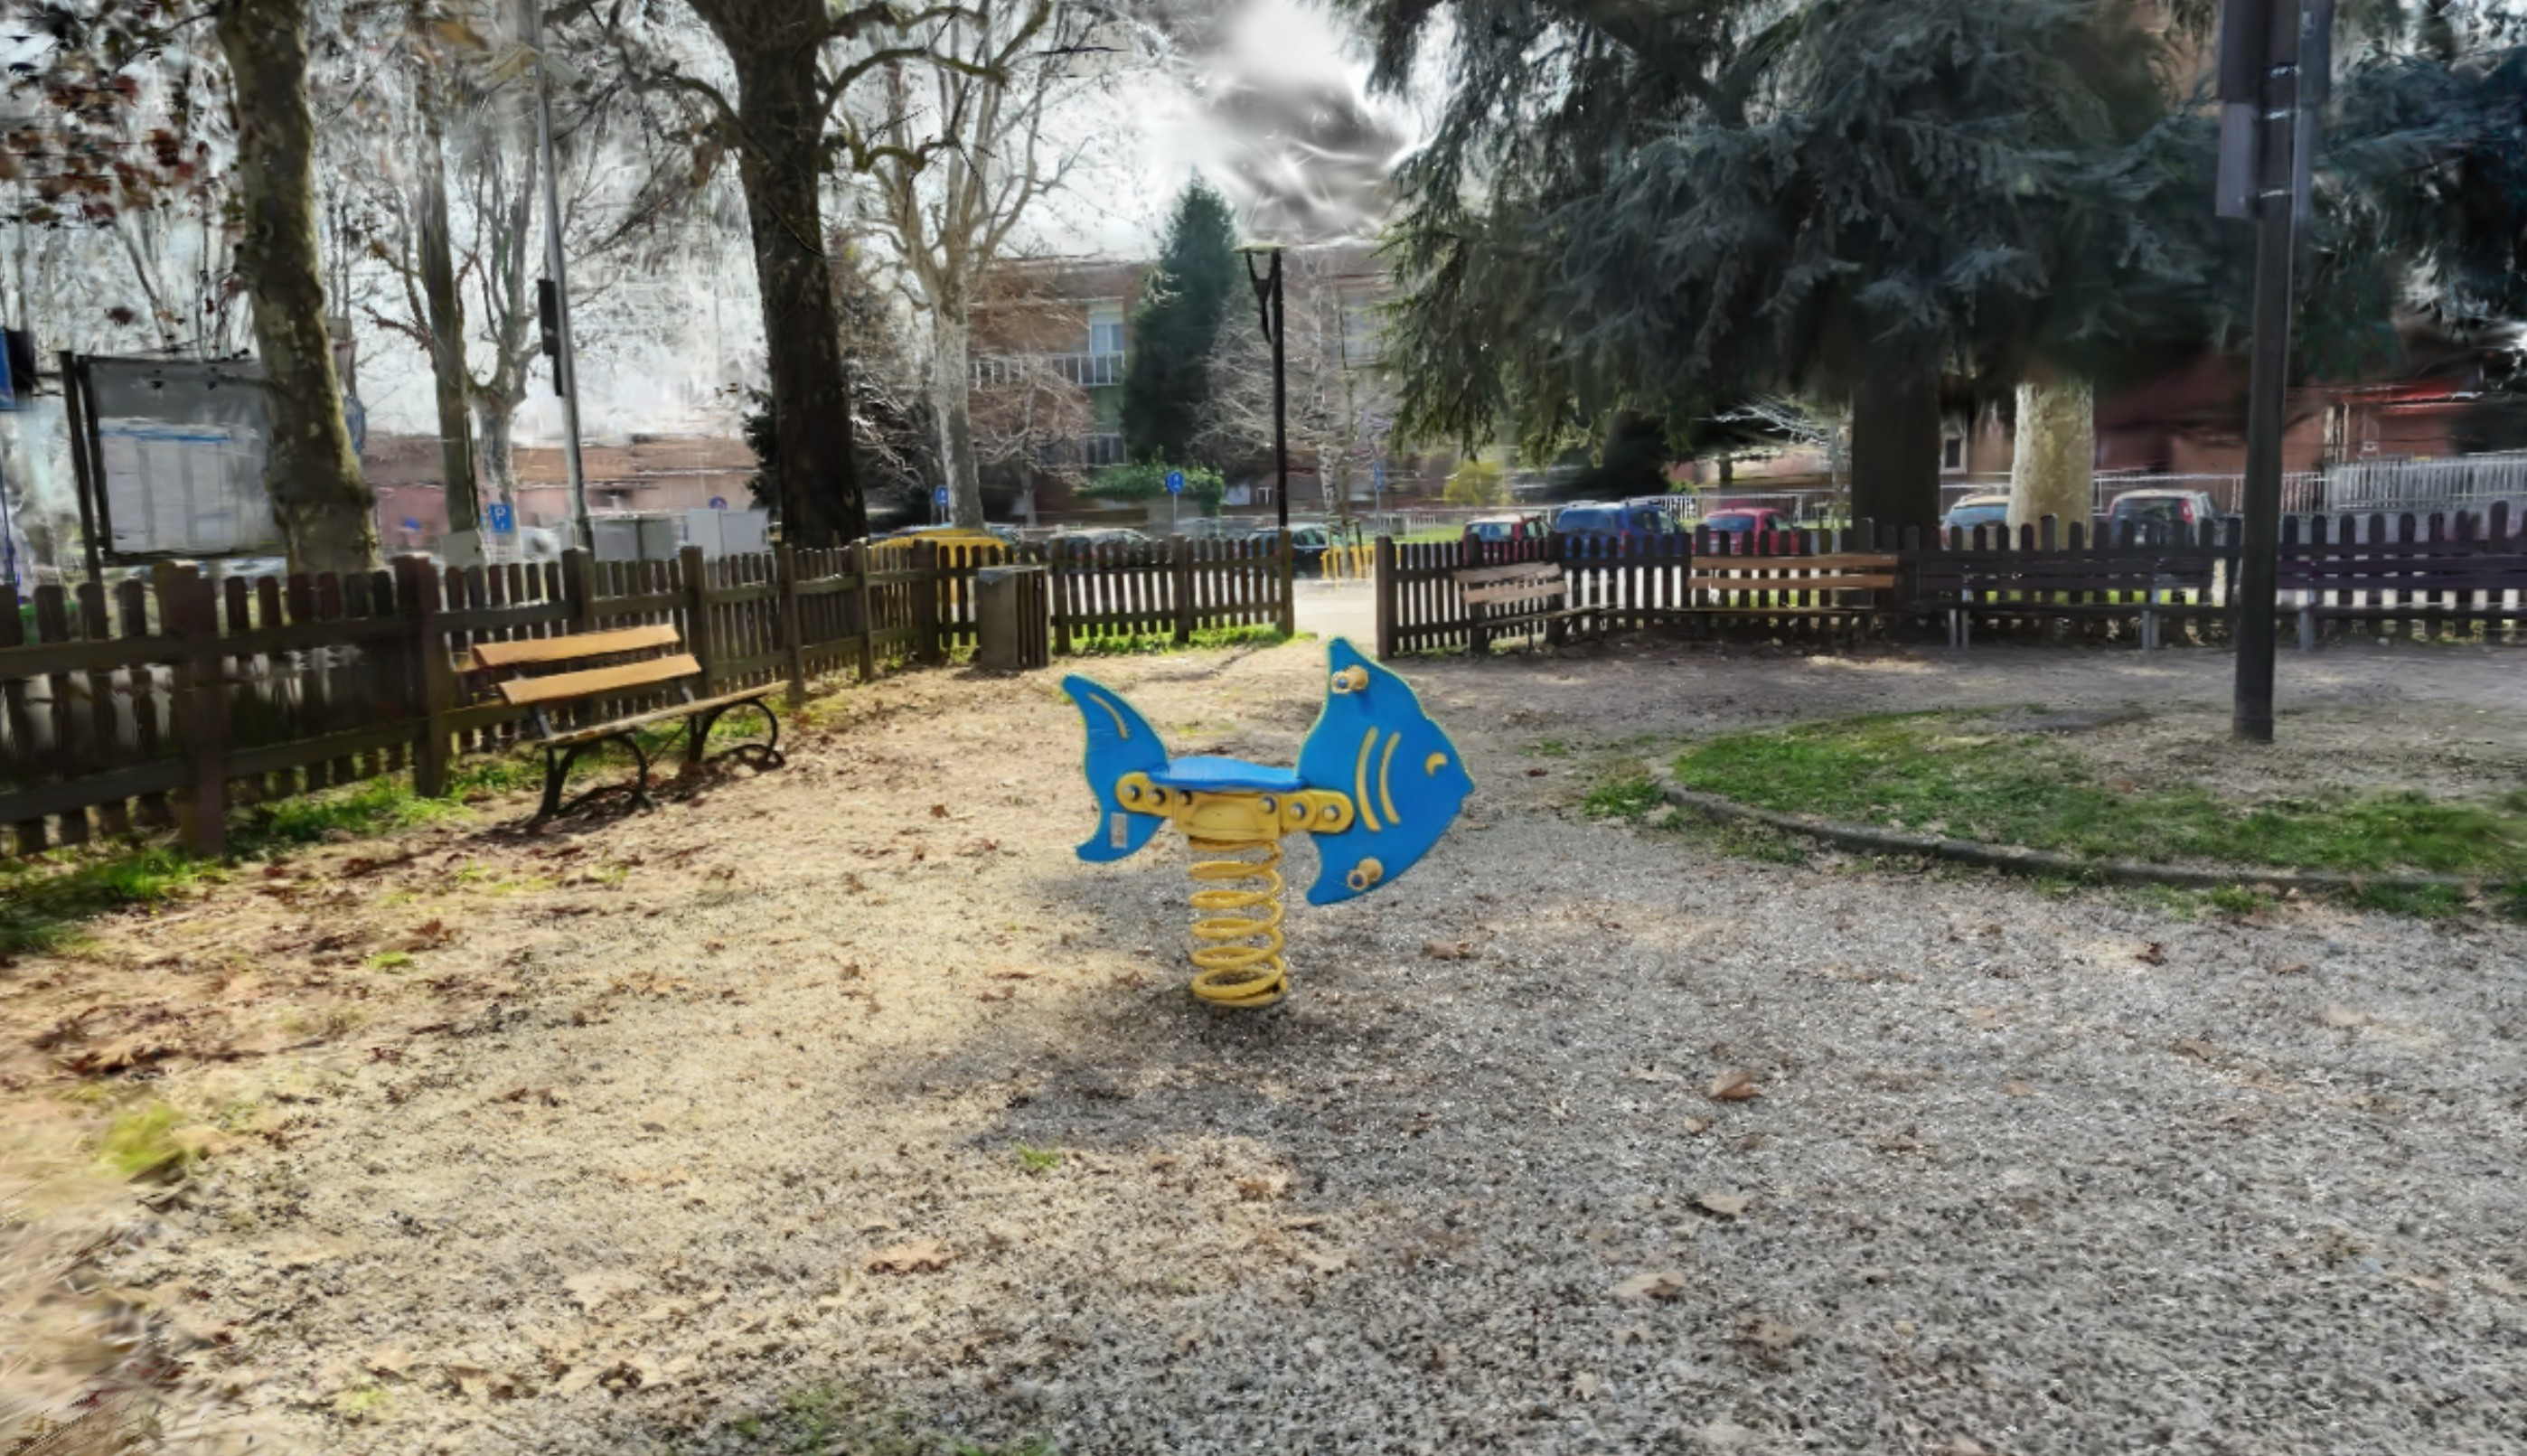
\includegraphics[width=0.32\textwidth,height=2.8cm,trim={80 40 80 40},clip]{images/benchmarks/spring_rider_inria_balanced_2.jpg}
	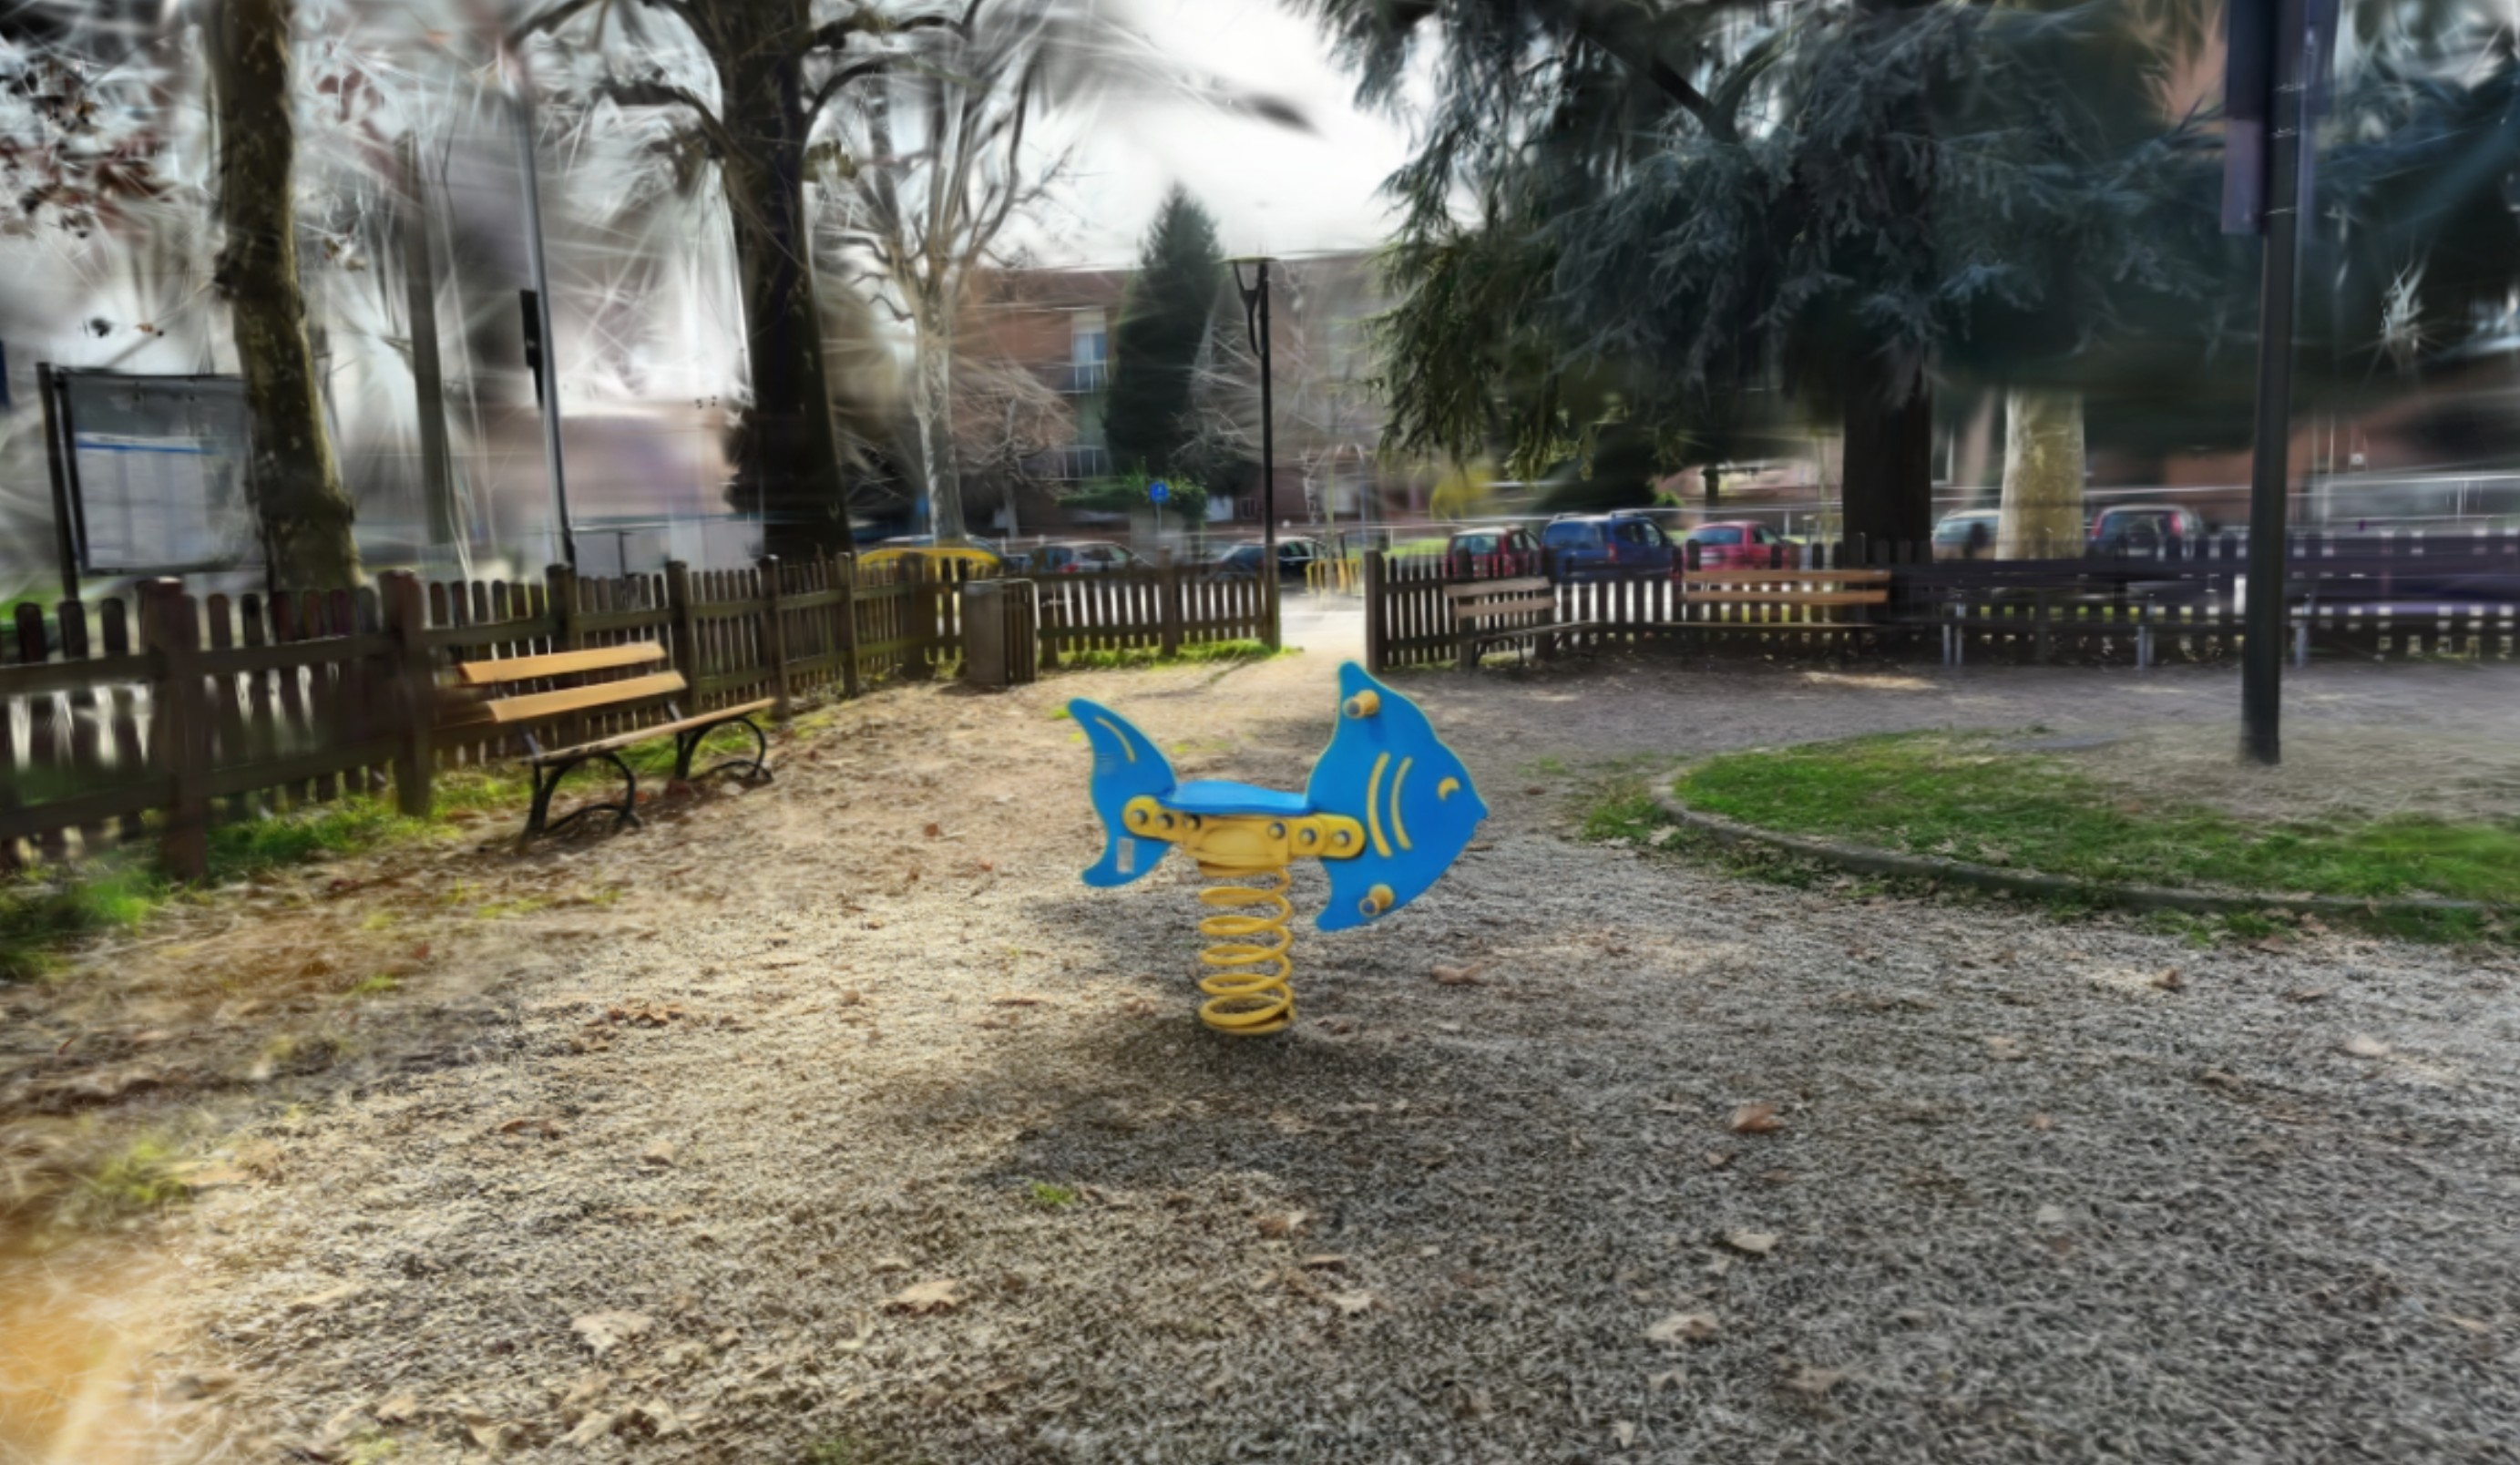
\includegraphics[width=0.32\textwidth,height=2.8cm,trim={80 40 80 40},clip]{images/benchmarks/spring_rider_mcmc_balanced_2.jpg}
	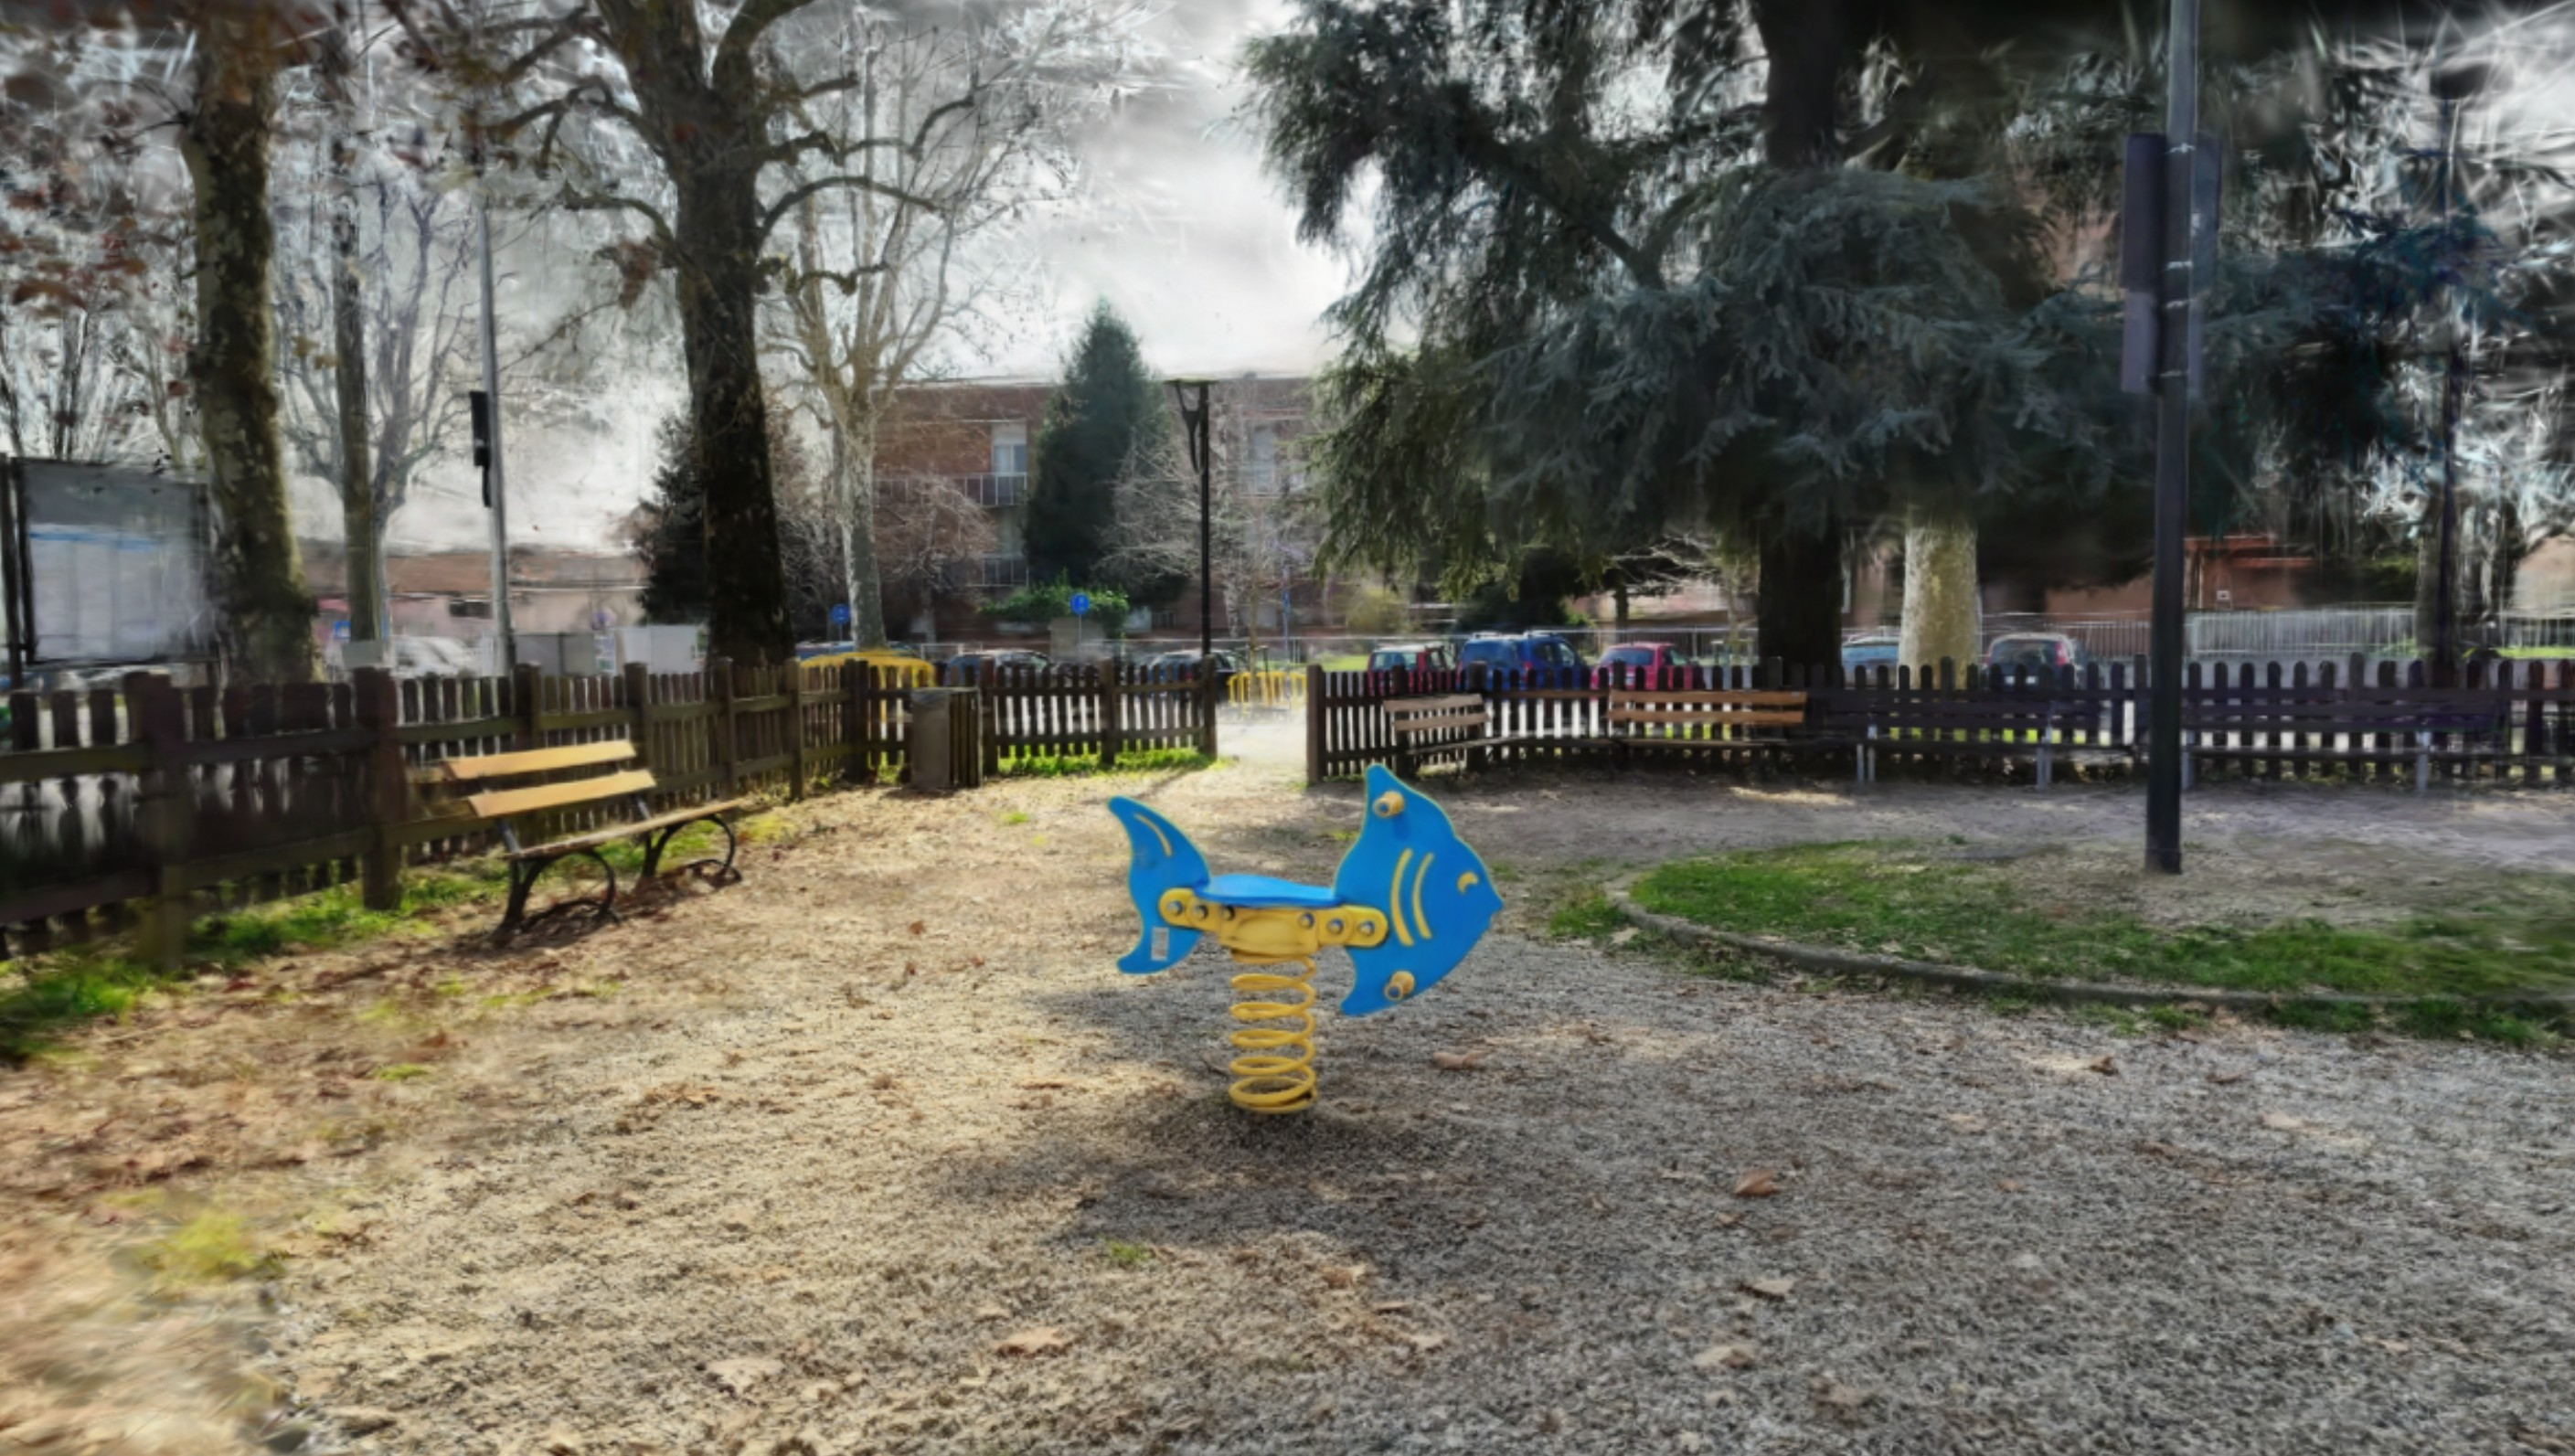
\includegraphics[width=0.32\textwidth,height=2.8cm,trim={80 40 80 40},clip]{images/benchmarks/spring_rider_taming_balanced_2.jpg}
	\caption{Confronto visivo Spring Rider (crop centrale) -- INRIA / MCMC / Taming}
	\label{fig:spring_rider_comparison}
\end{figure}


\begin{figure}[ht]
	\centering
	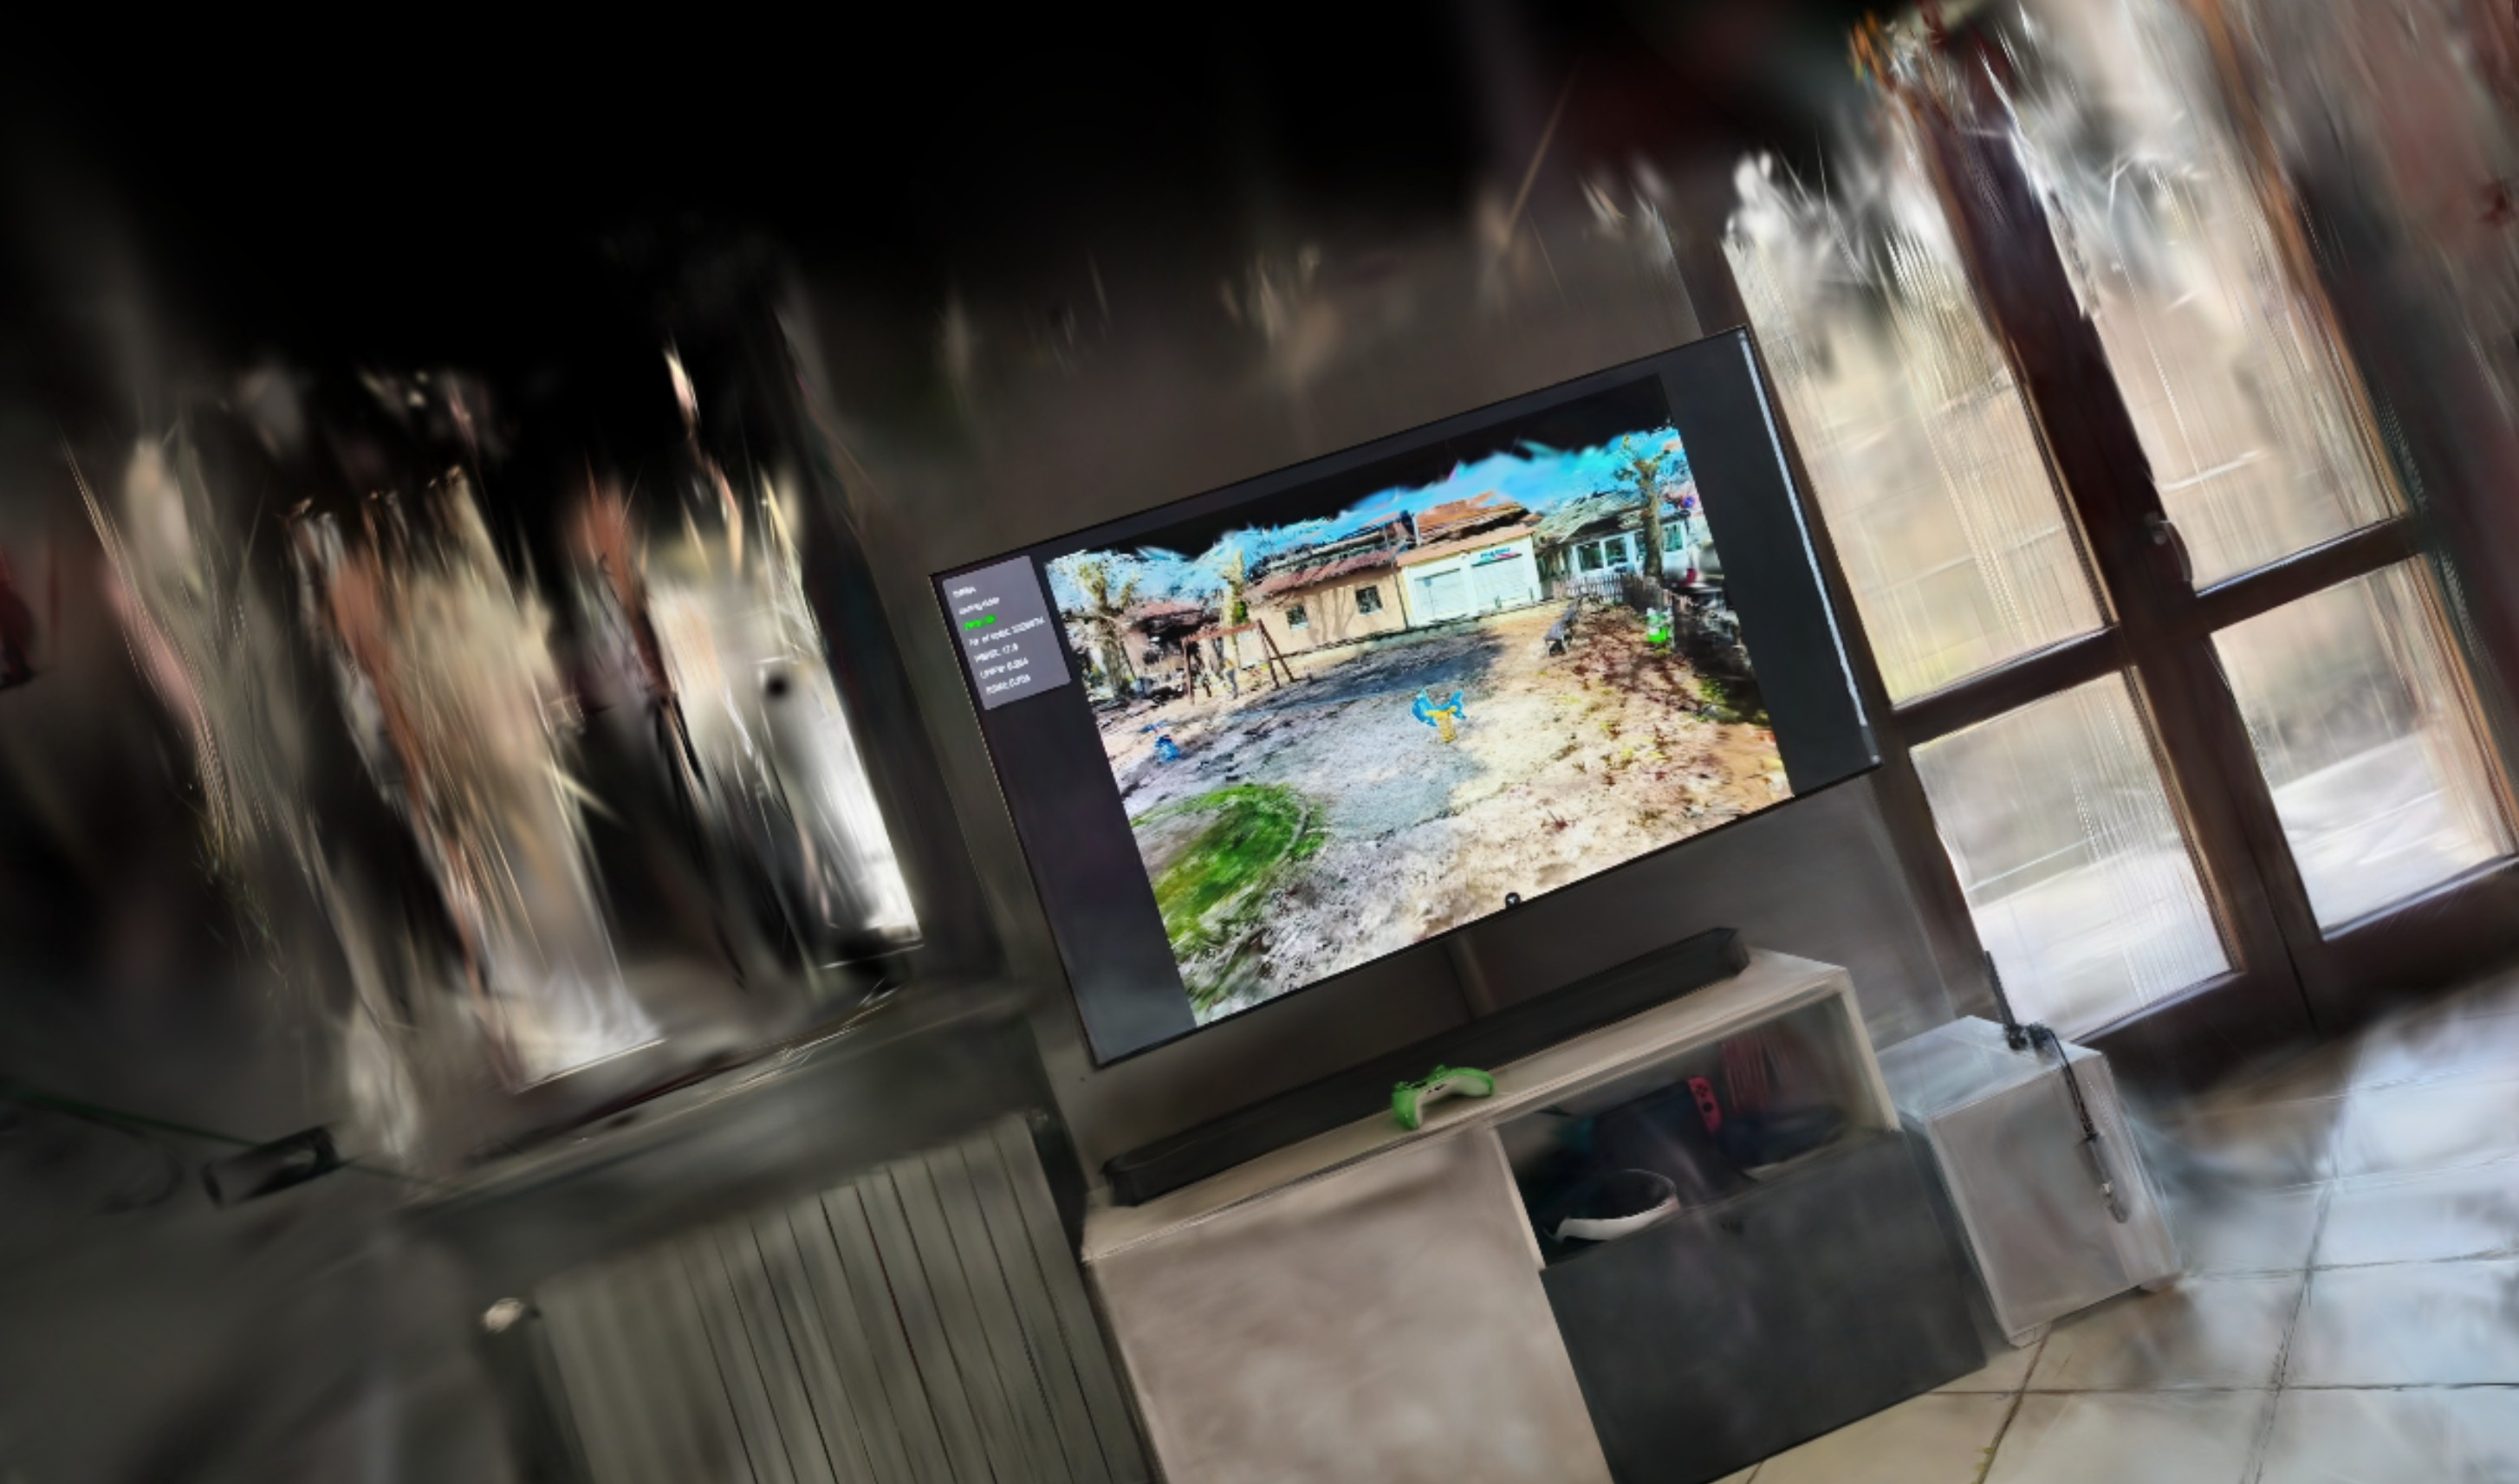
\includegraphics[width=0.32\textwidth,height=2.8cm,trim={80 40 80 40},clip]{images/benchmarks/my_workstation_inria_balanced_1.jpg}
	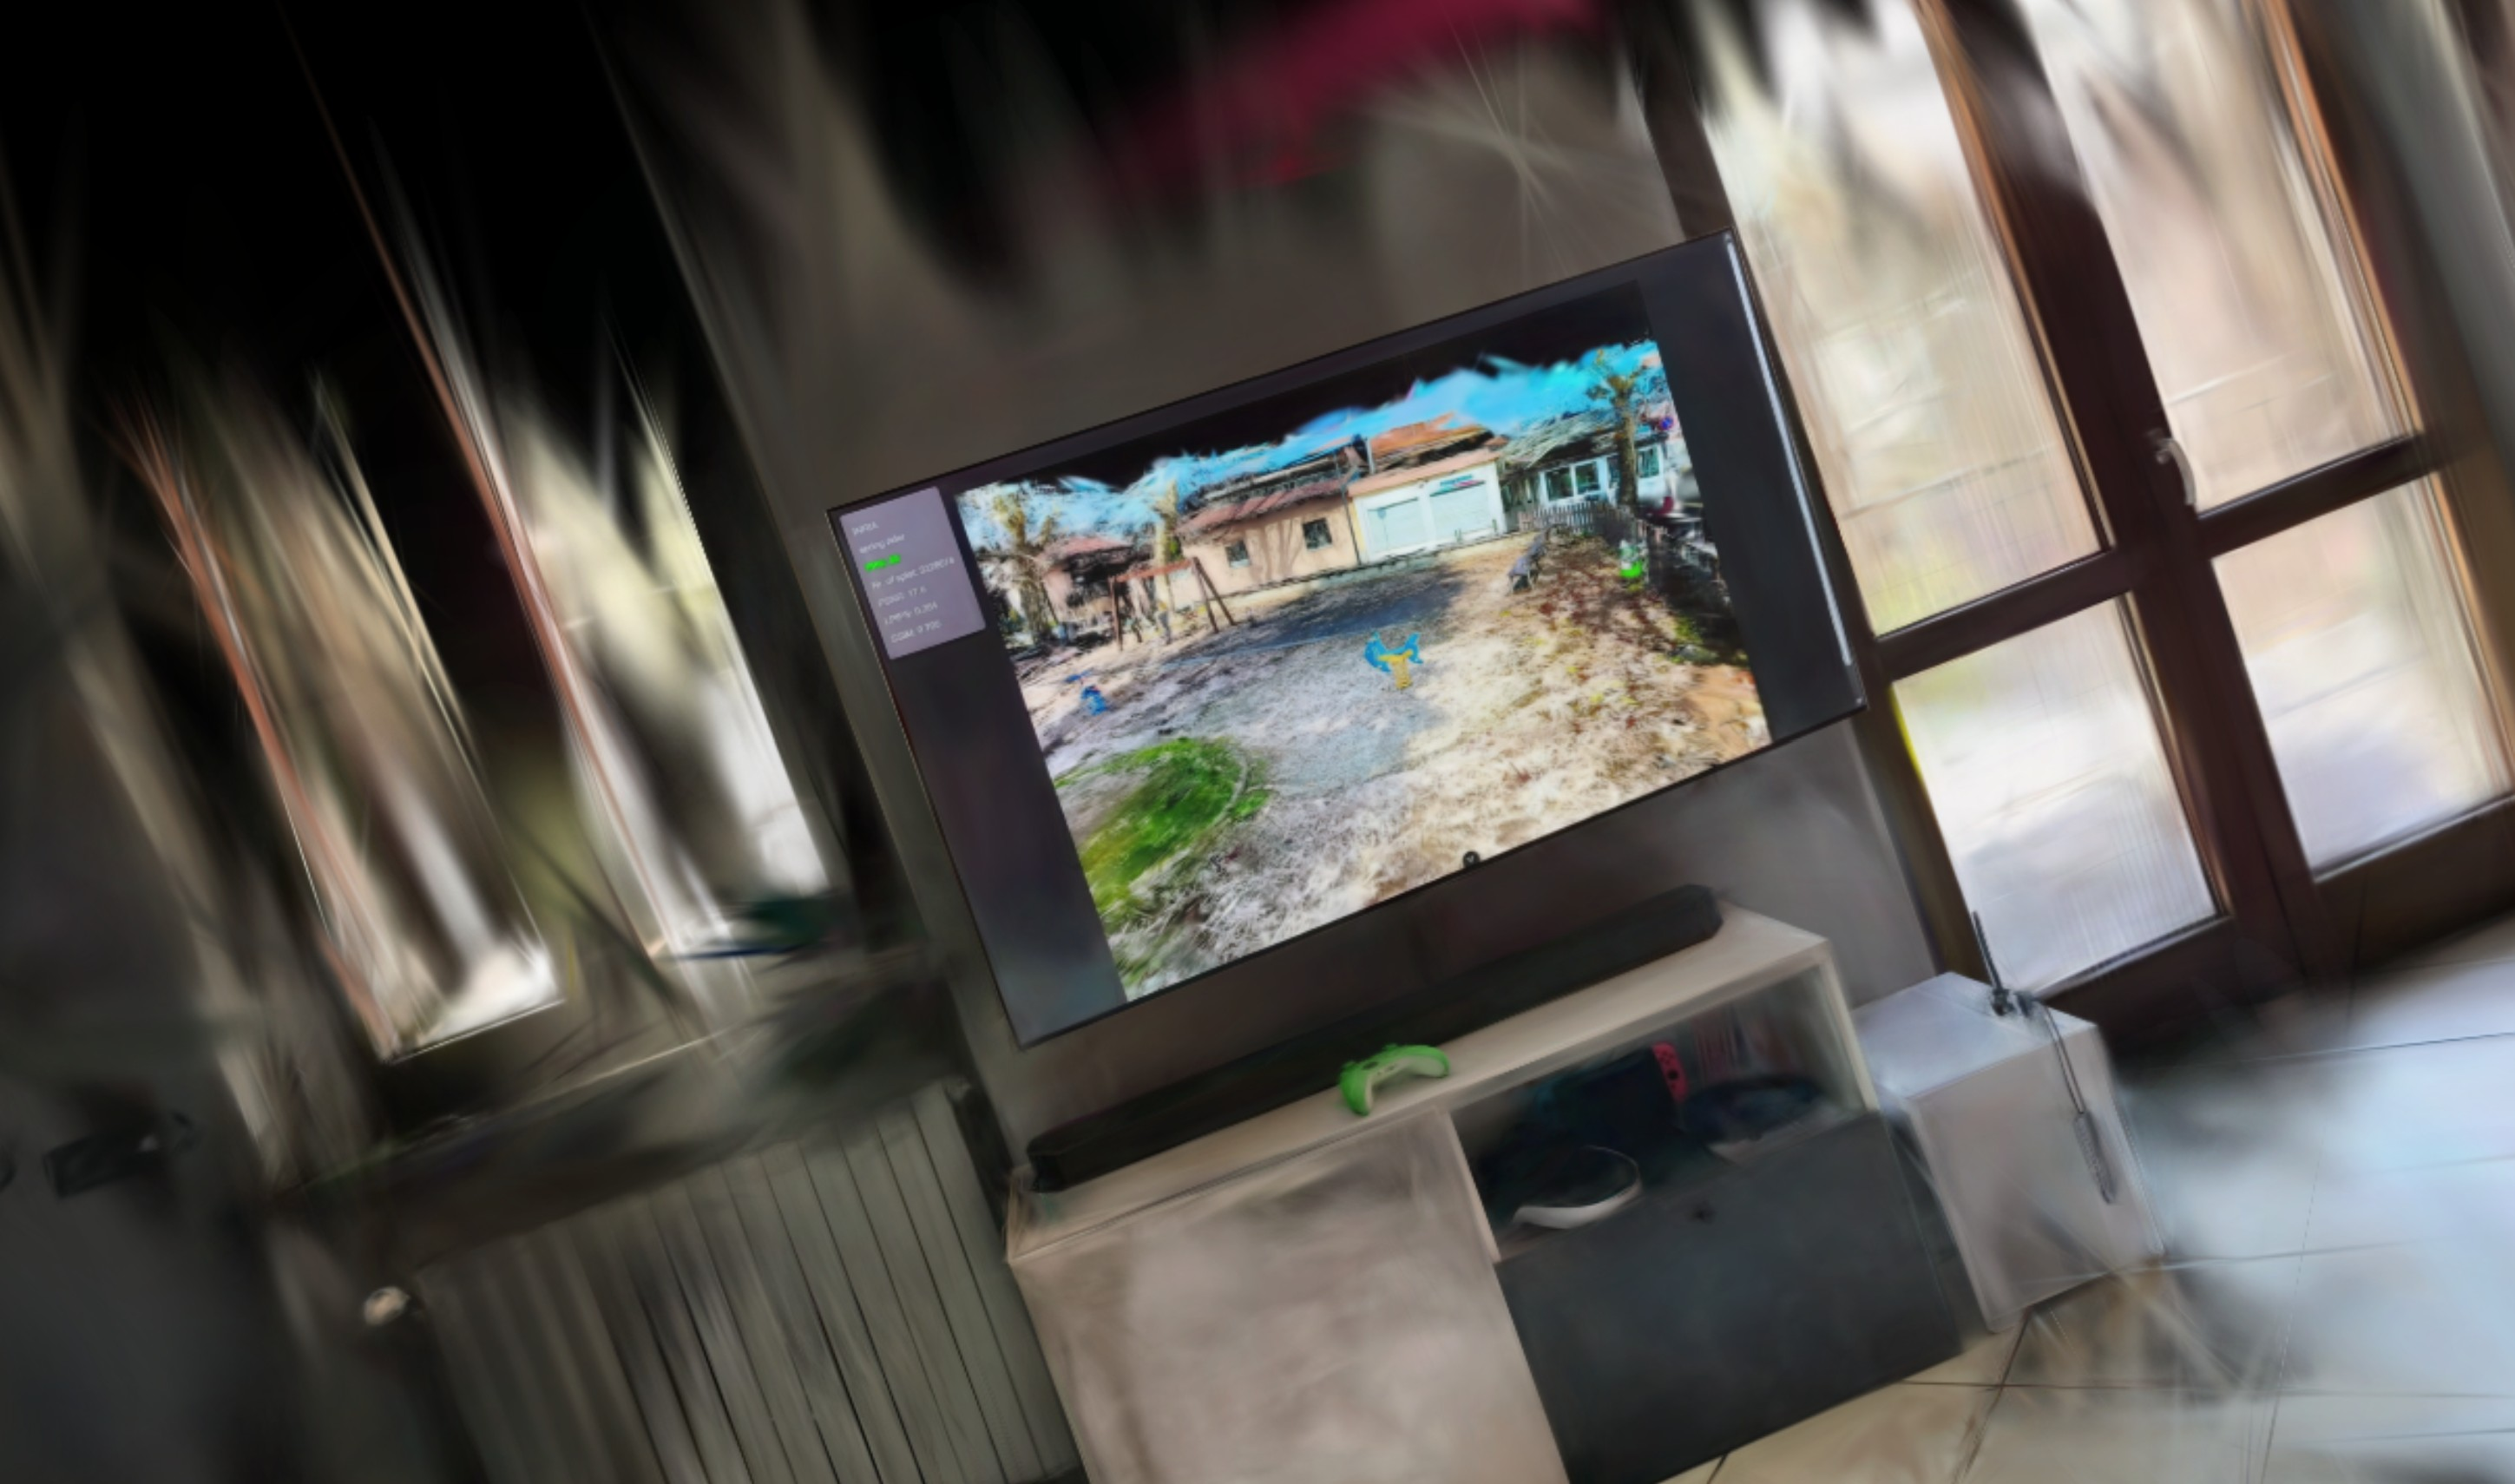
\includegraphics[width=0.32\textwidth,height=2.8cm,trim={80 40 80 40},clip]{images/benchmarks/my_workstation_mcmc_balanced_1.jpg}
	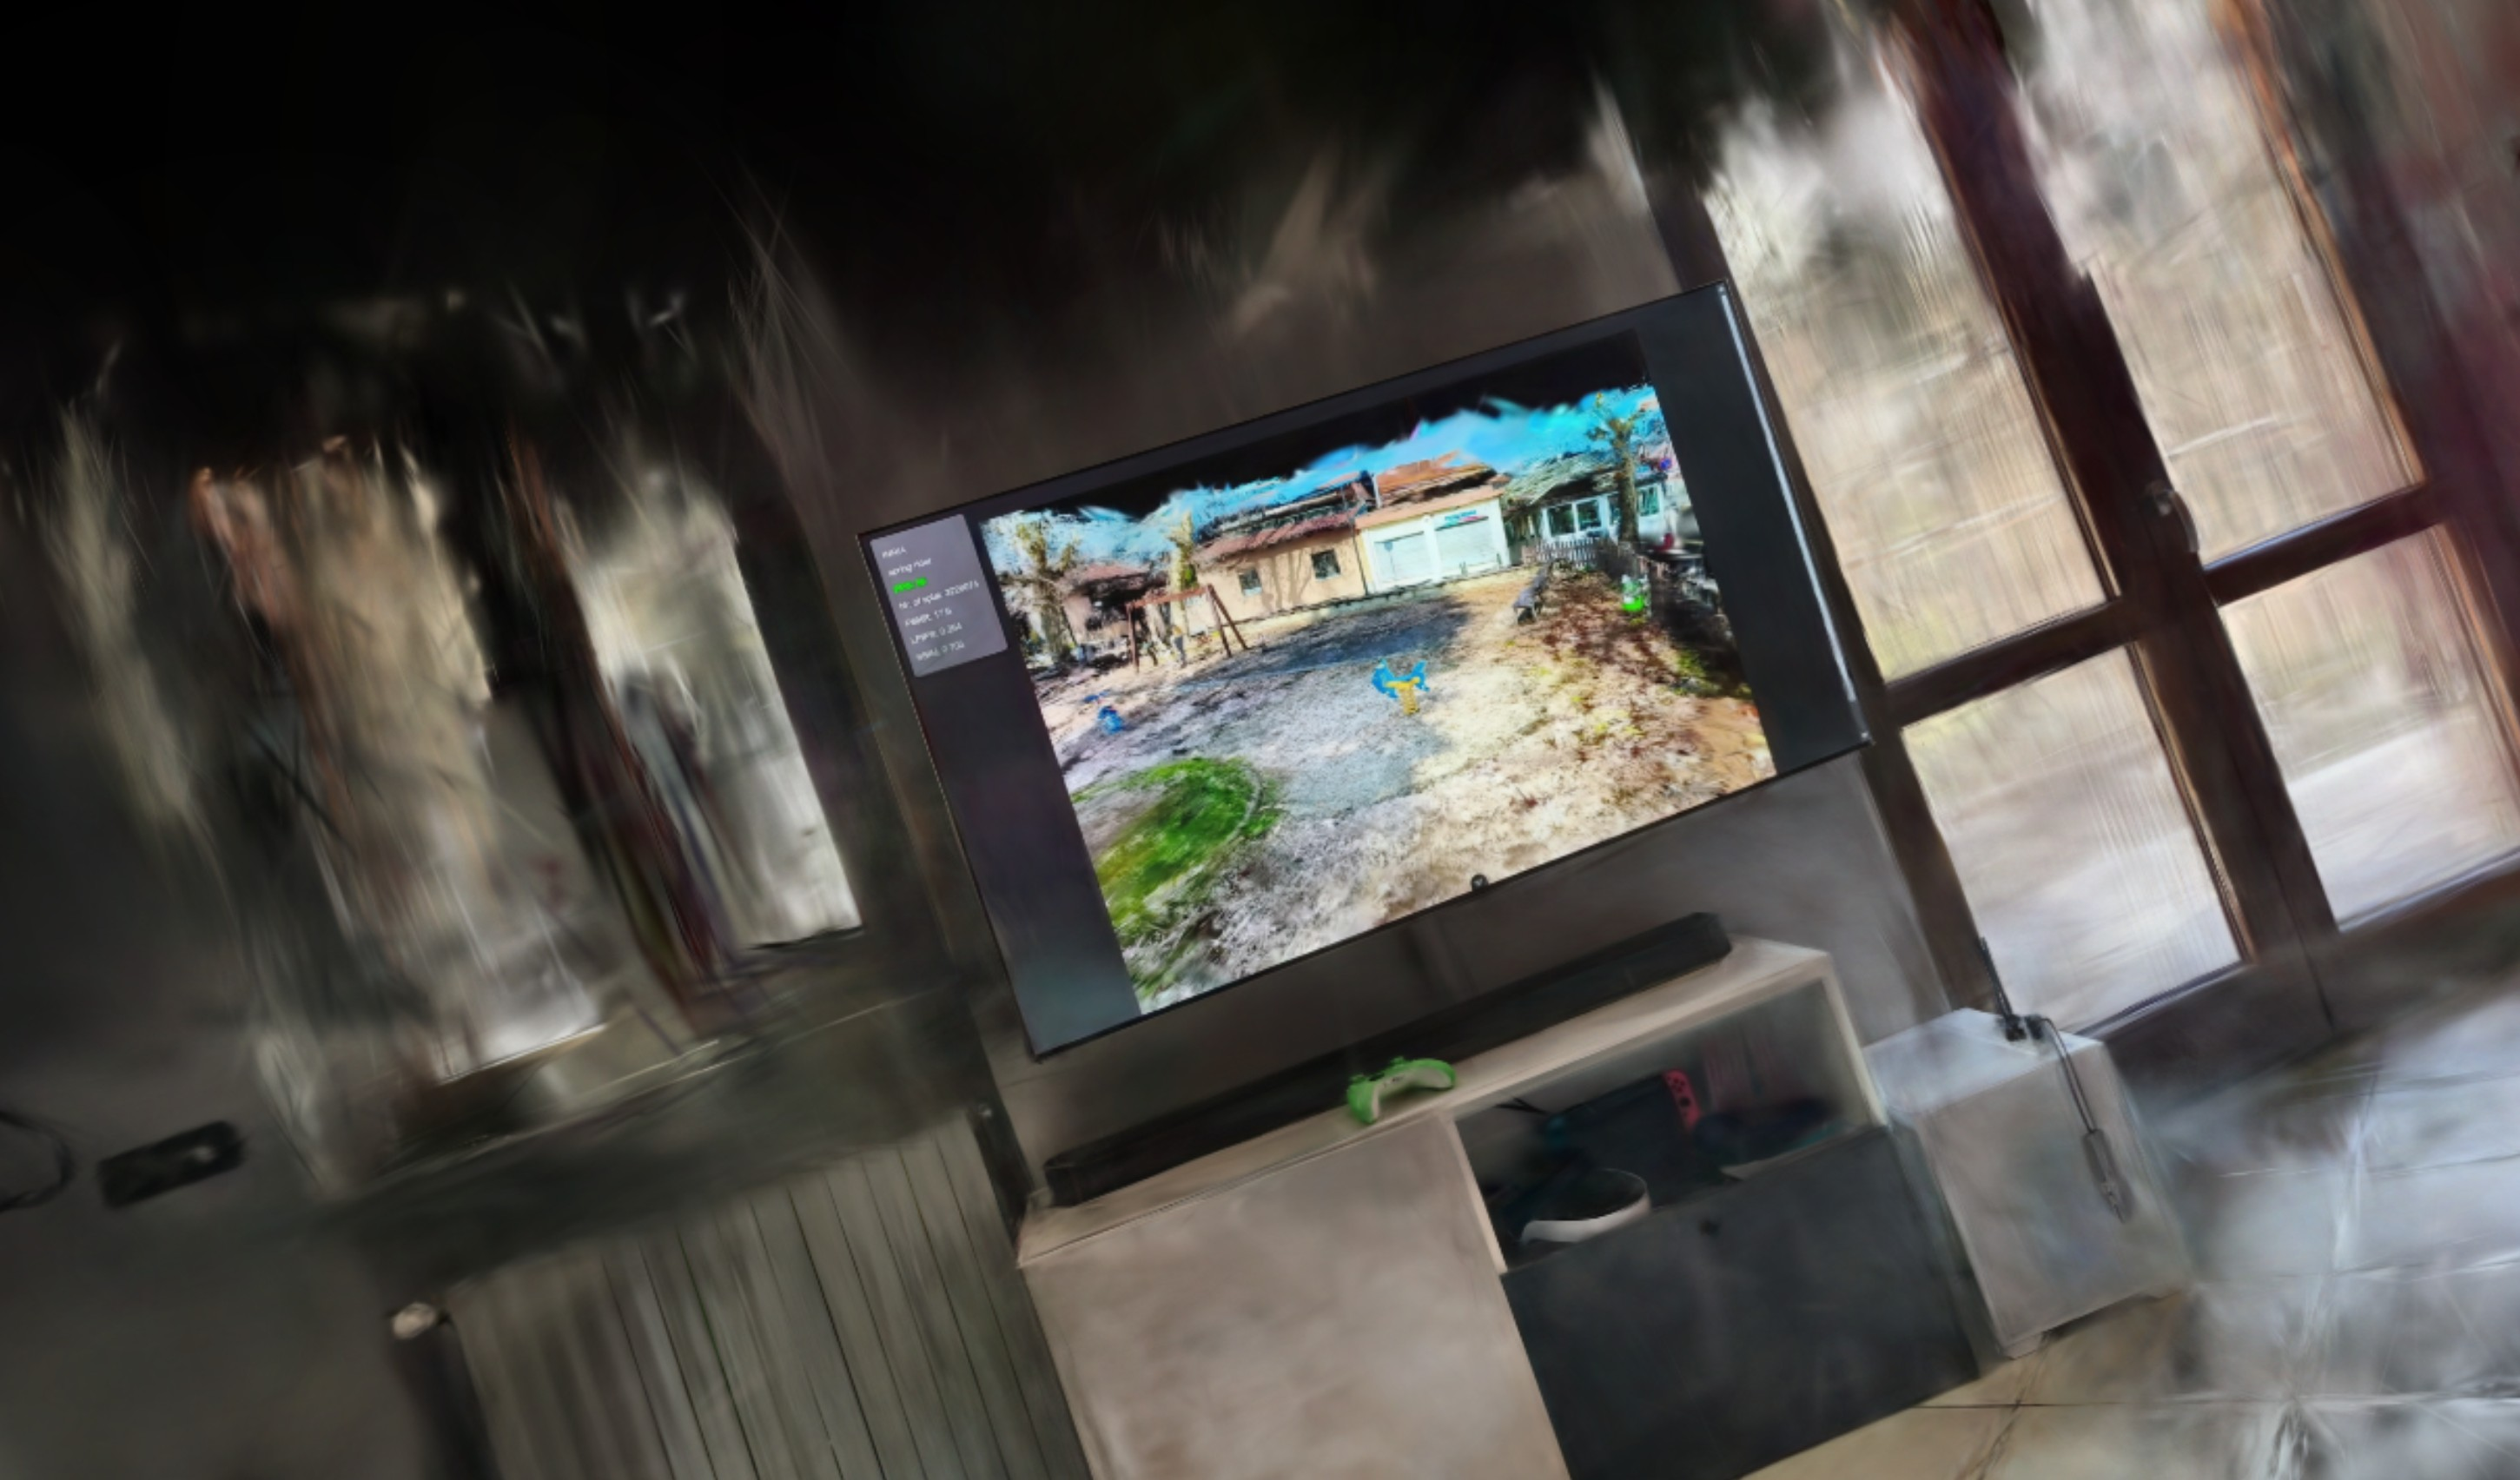
\includegraphics[width=0.32\textwidth,height=2.8cm,trim={80 40 80 40},clip]{images/benchmarks/my_workstation_taming_balanced_1.jpg}
		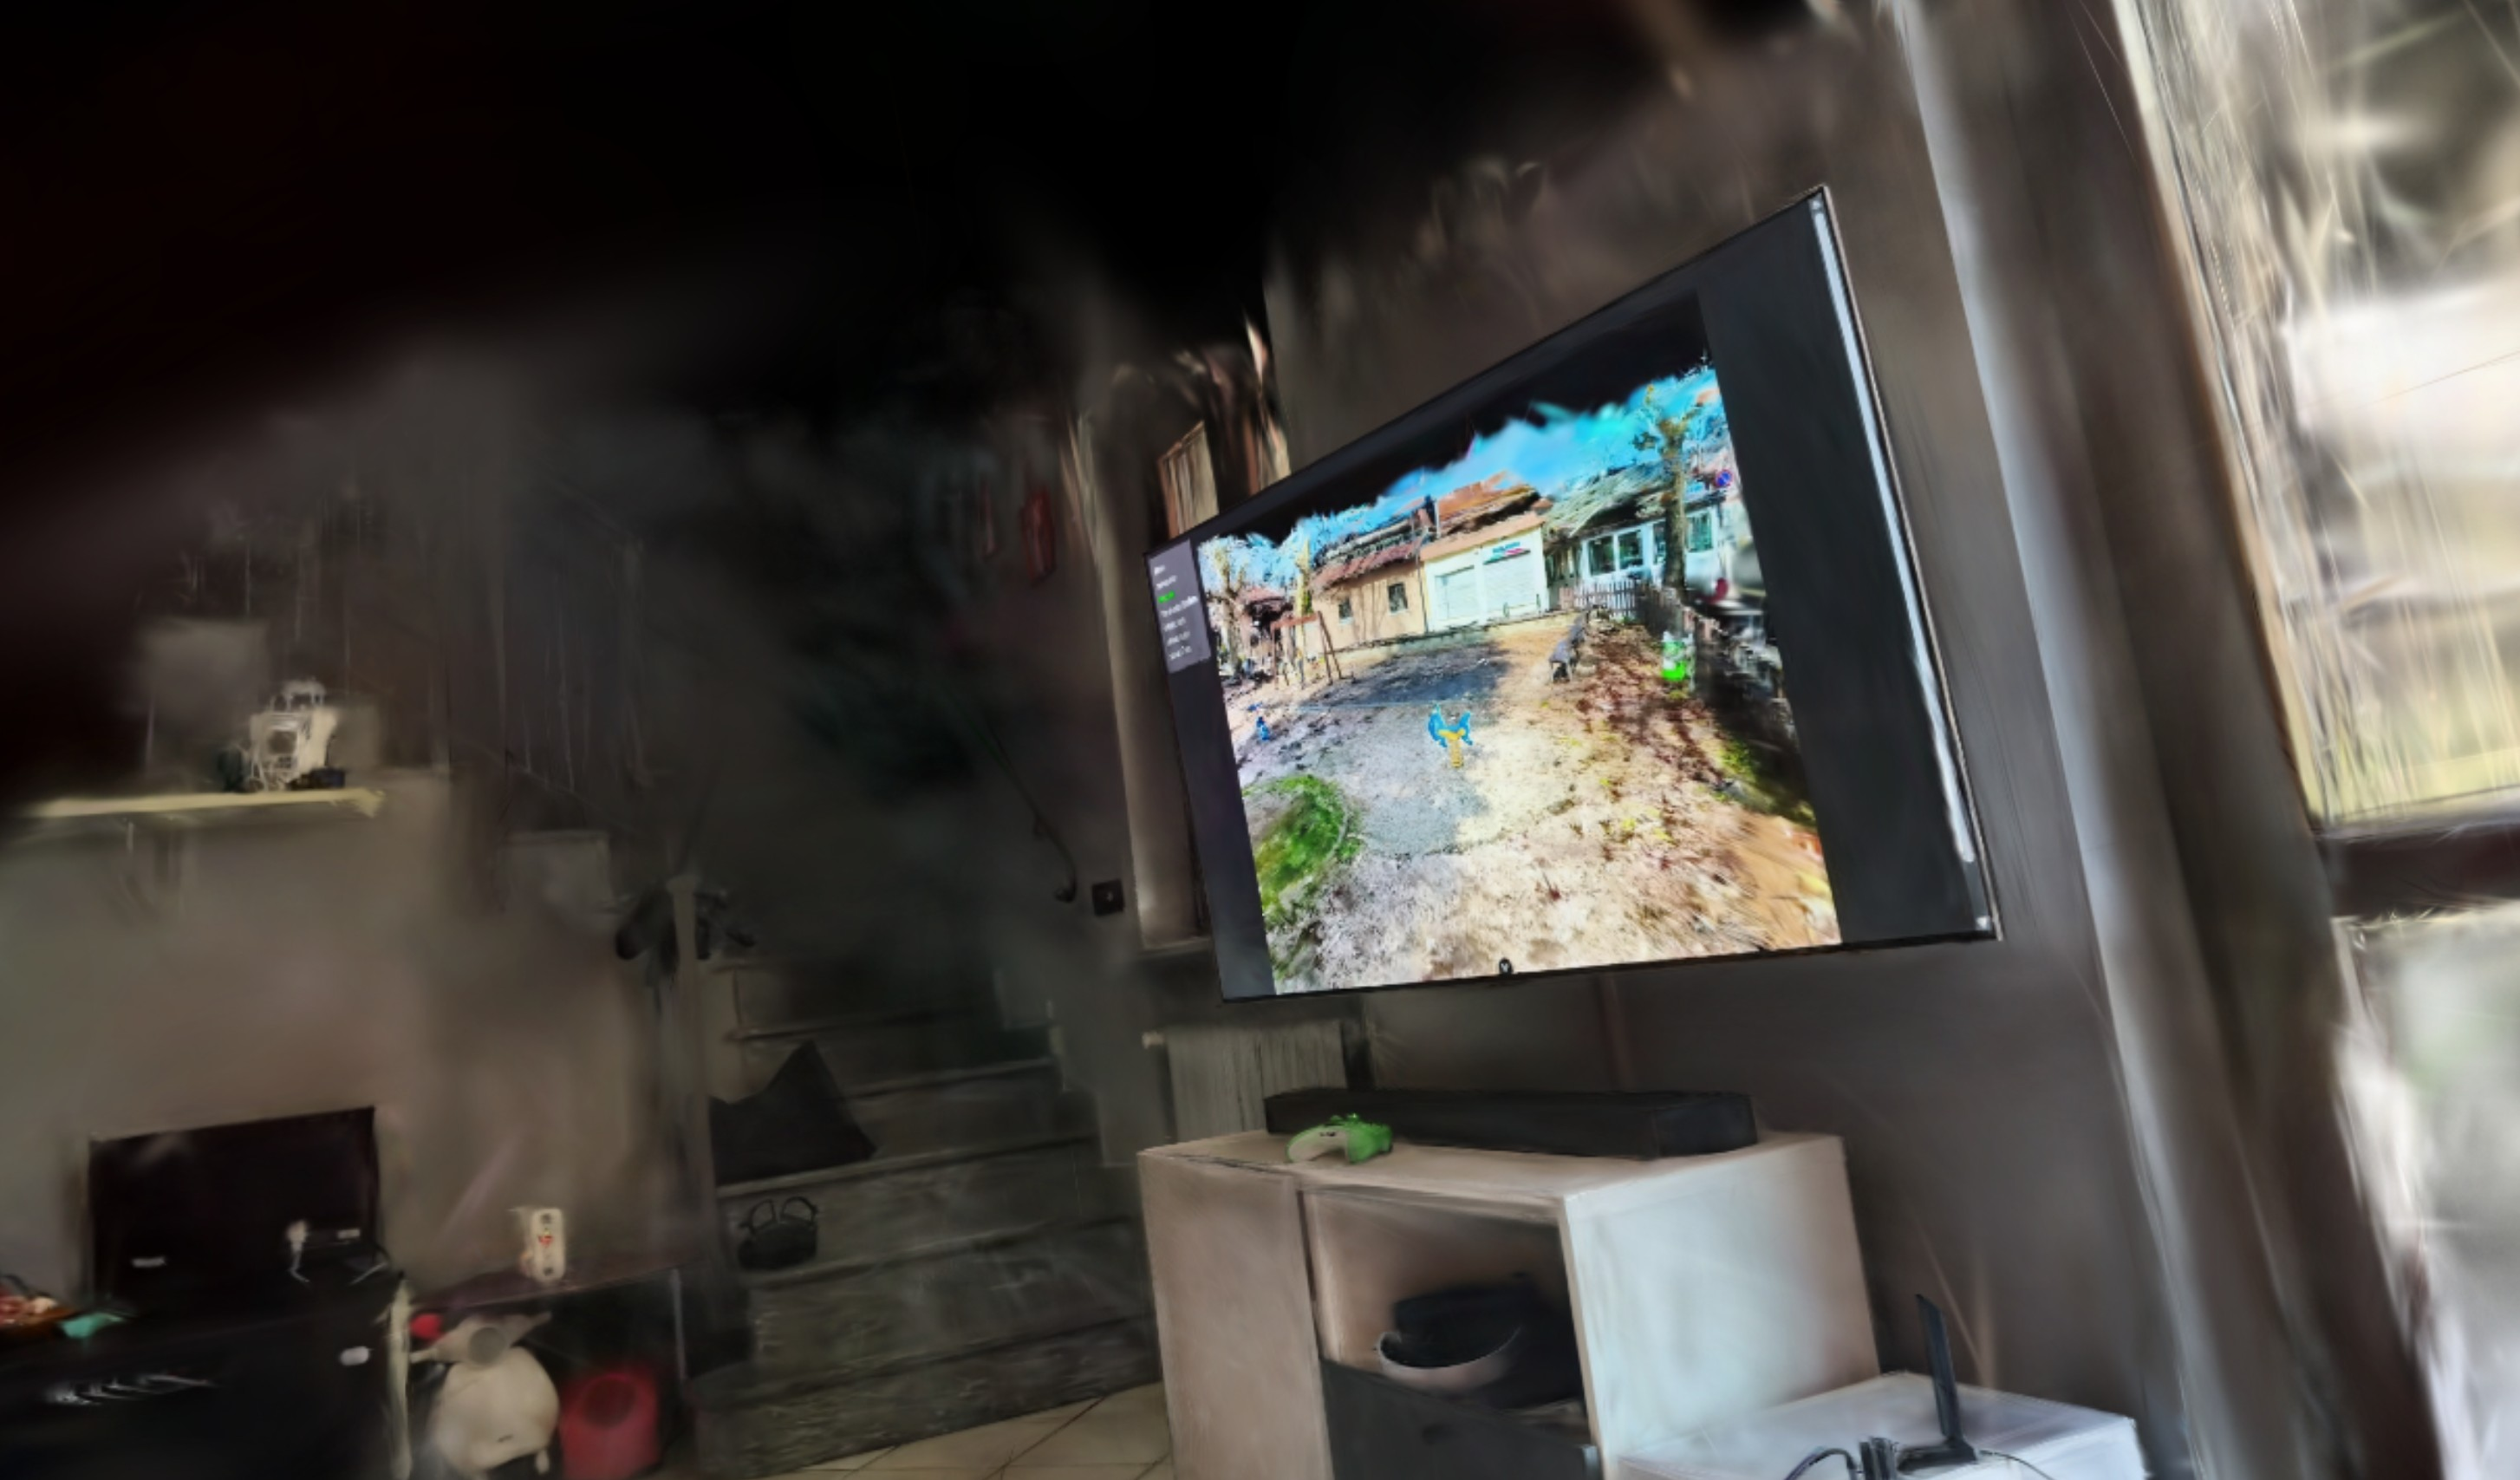
\includegraphics[width=0.32\textwidth,height=2.8cm,trim={80 40 80 40},clip]{images/benchmarks/my_workstation_inria_balanced_2.jpg}
	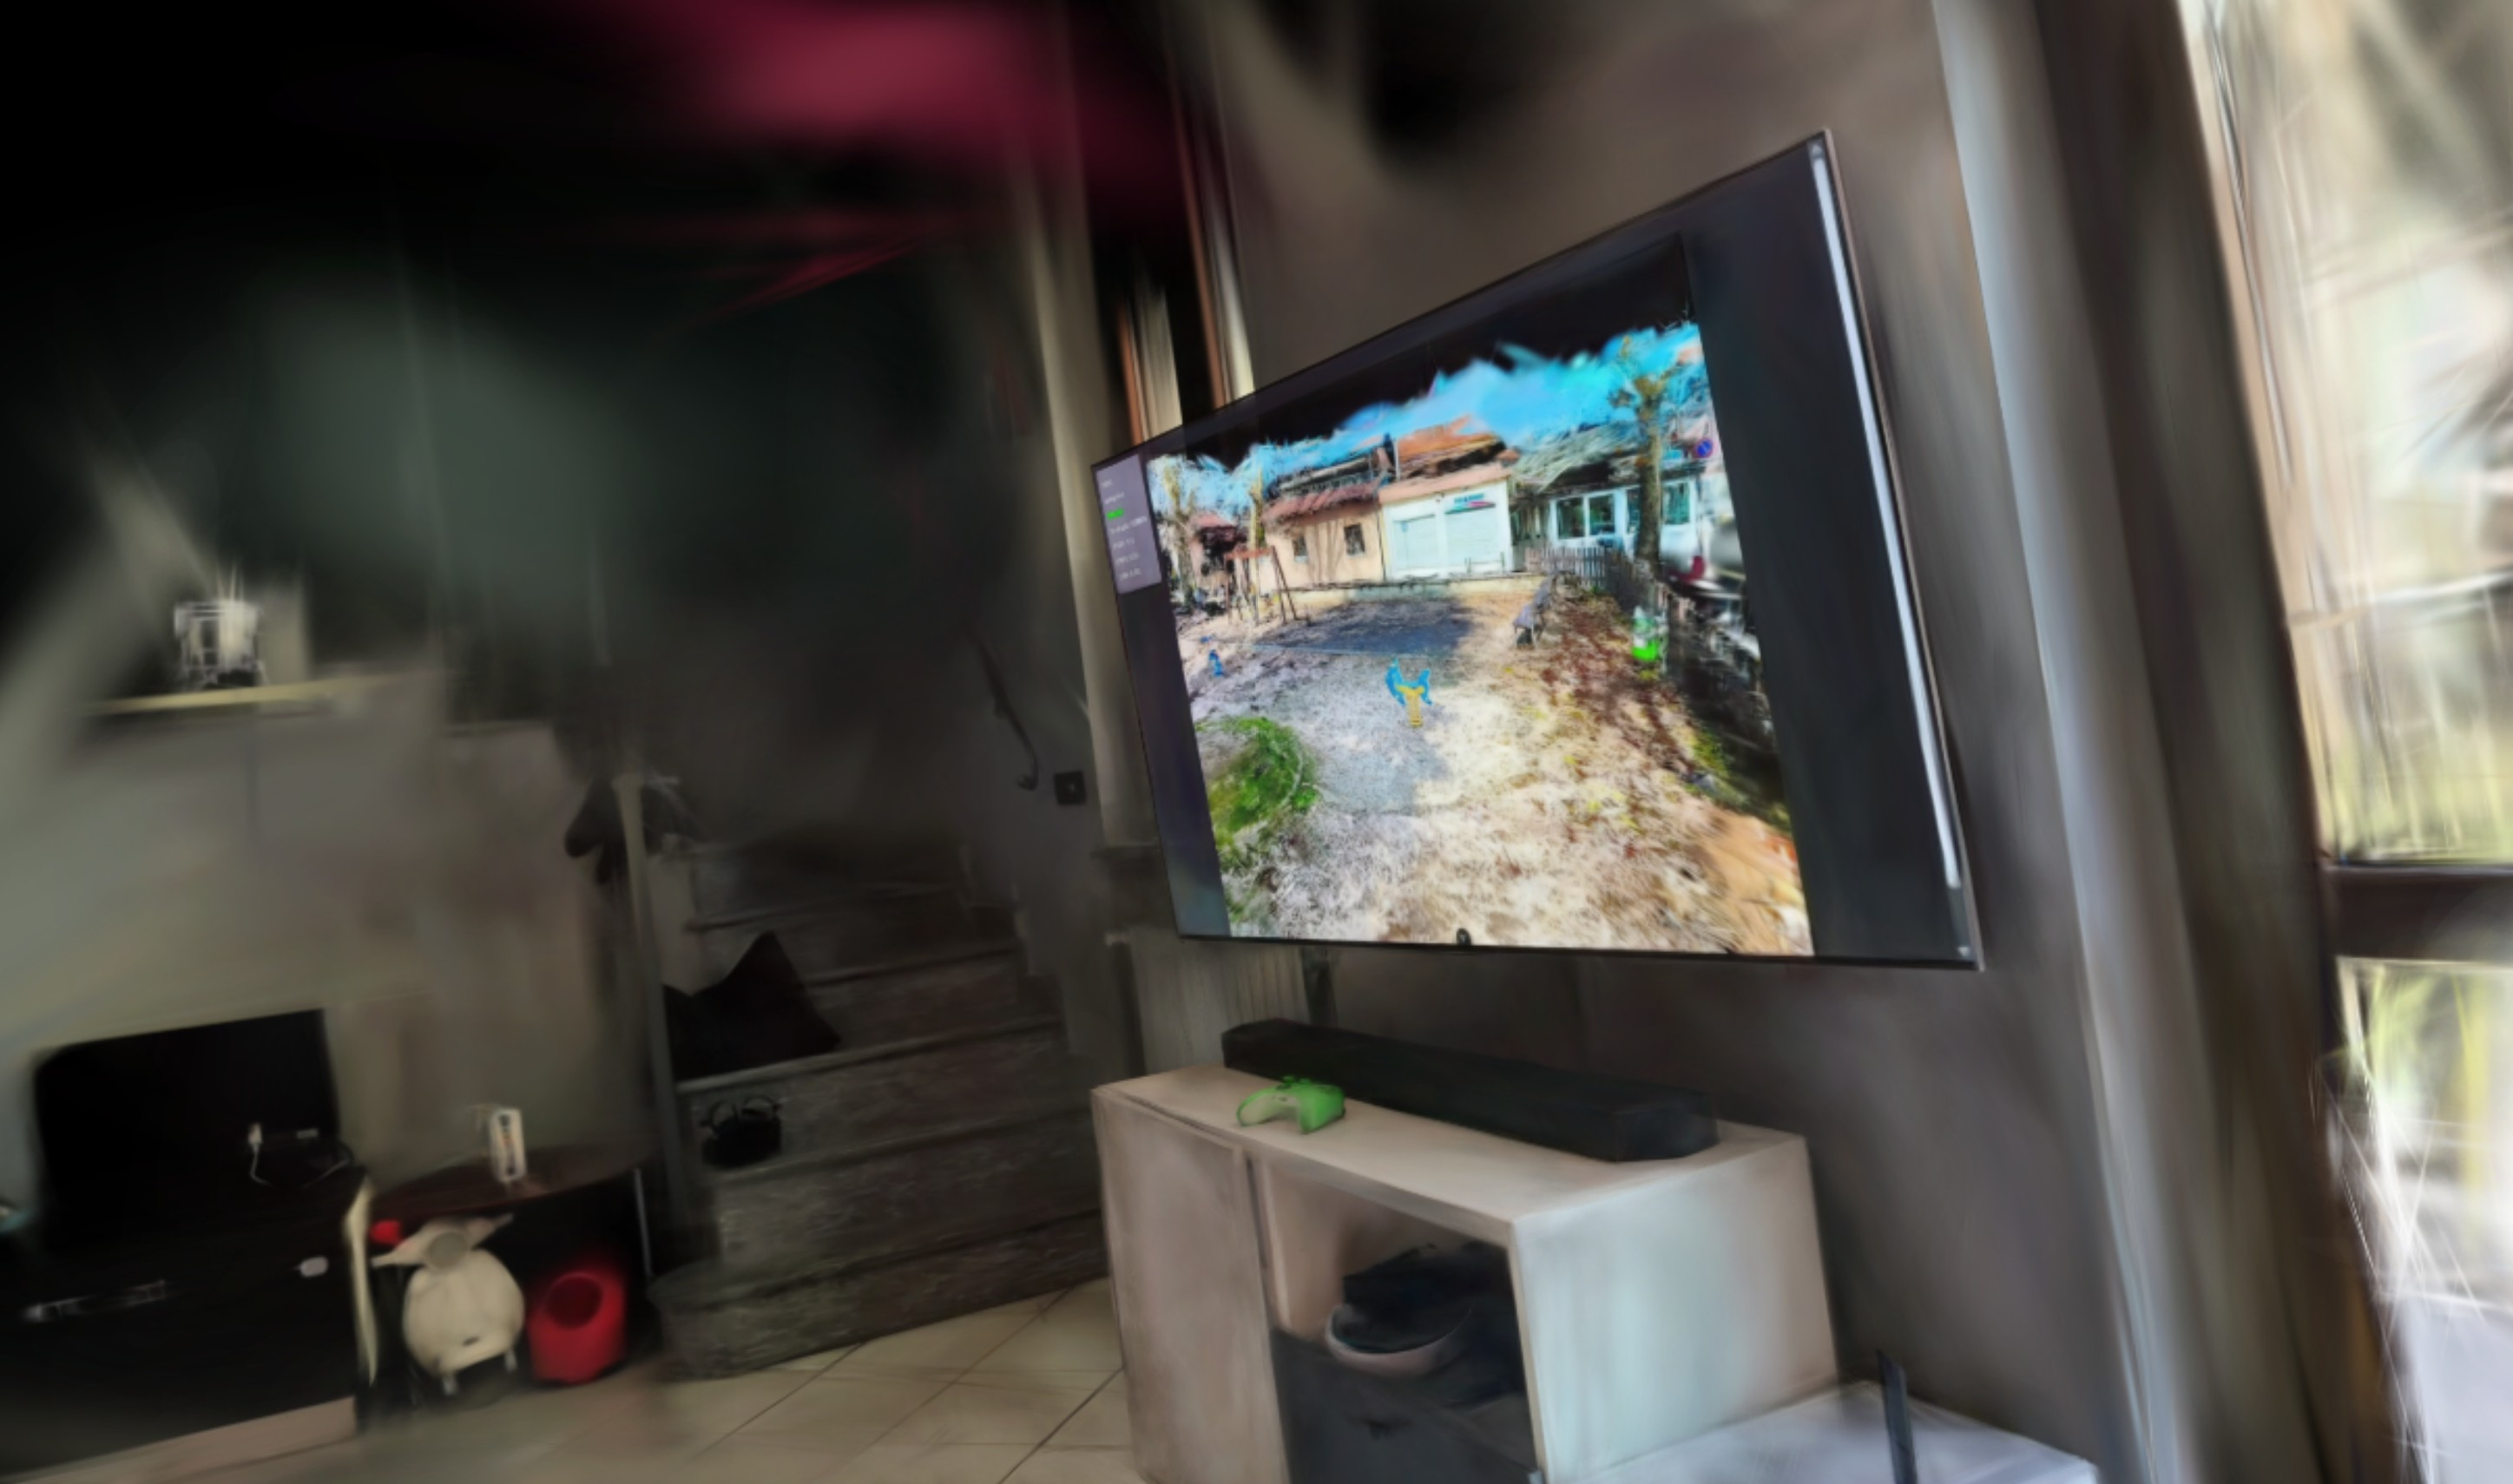
\includegraphics[width=0.32\textwidth,height=2.8cm,trim={80 40 80 40},clip]{images/benchmarks/my_workstation_mcmc_balanced_2.jpg}
	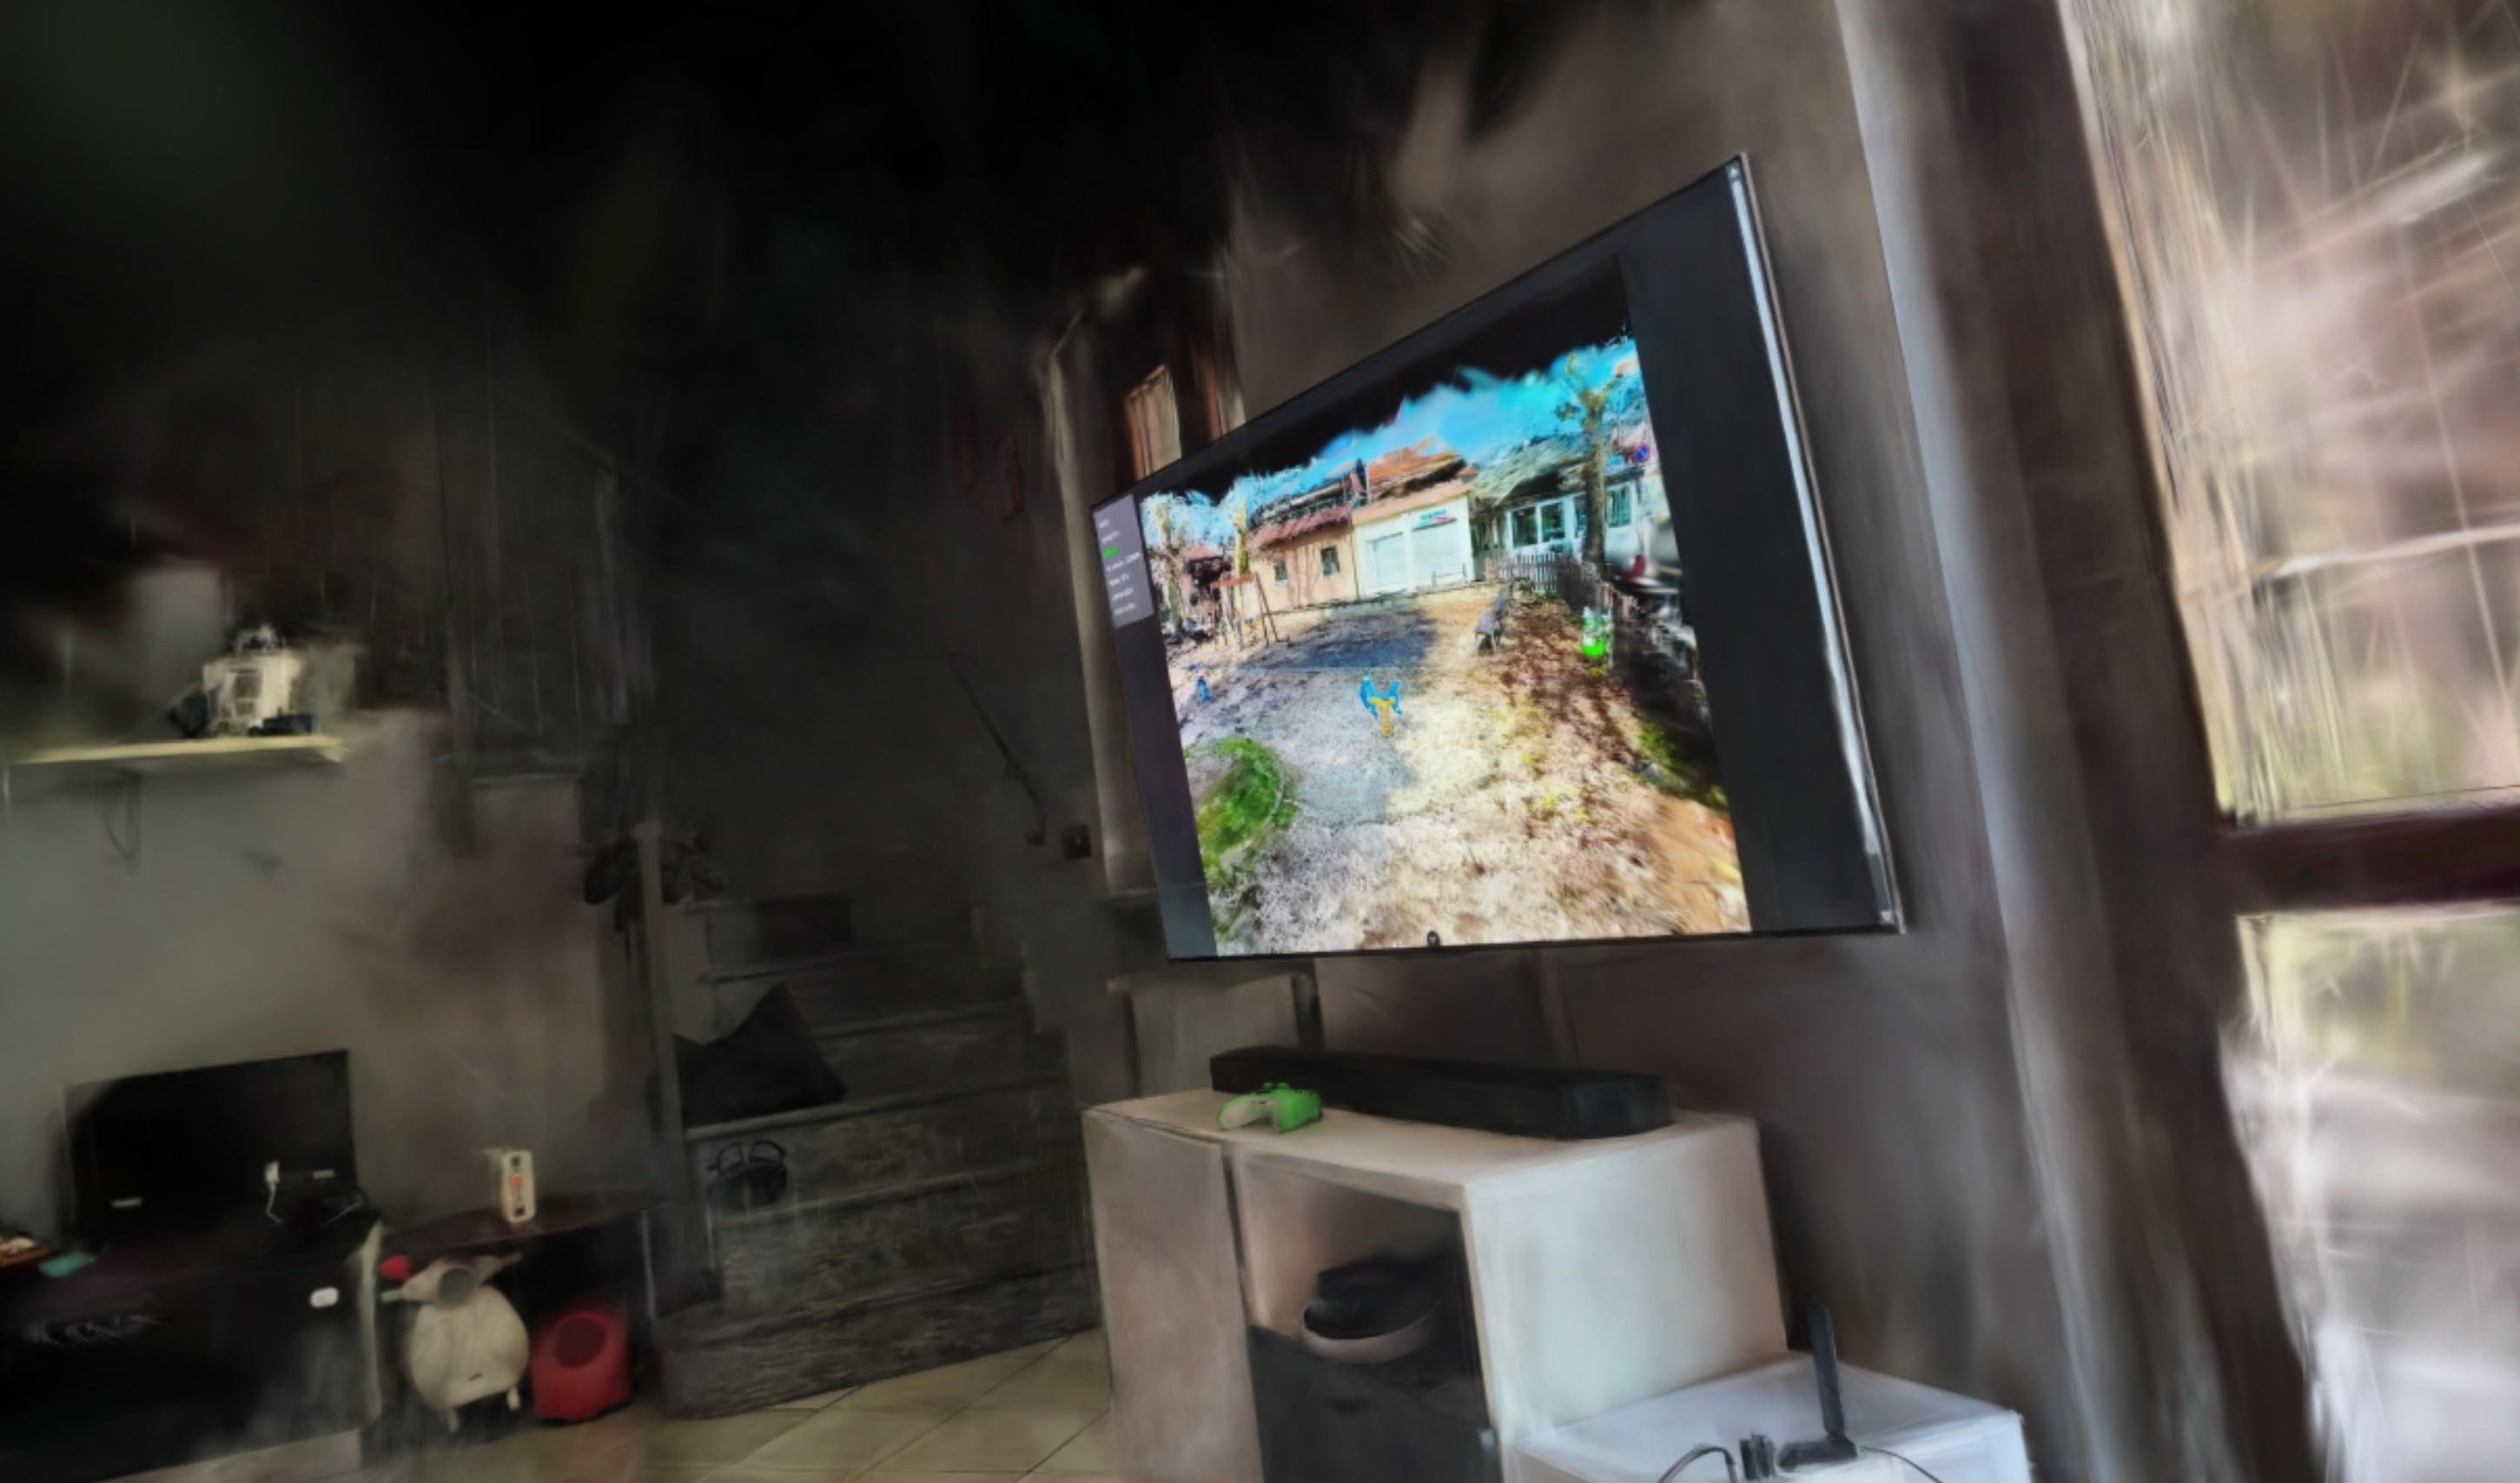
\includegraphics[width=0.32\textwidth,height=2.8cm,trim={80 40 80 40},clip]{images/benchmarks/my_workstation_taming_balanced_2.jpg}
	\caption{Confronto visivo My workstation (crop centrale) -- INRIA / MCMC / Taming}
	\label{fig:my_workstation_comparison}
\end{figure}



\paragraph{Tabella comparativa qualitativa}
\begin{table}[H]
	\centering
	\caption{Sintesi qualitativa visuale (S1 \textit{Spring Rider} e S3 \textit{My Workstation})}
	\label{tab:benchmark1_quality_visual}
	\begin{tabularx}{\linewidth}{l >{\centering\arraybackslash}X >{\centering\arraybackslash}X >{\centering\arraybackslash}X}
		\toprule
		\textbf{Criterio} & \textbf{INRIA} & \textbf{MCMC} & \textbf{Taming} \\
		\midrule
		Nitidezza soggetto / oggetti vicini & \warn & \cmark & \cmark \\
		Fedeltà cromatica                   & \warn & \warn  & \cmark \\
		Dettagli sfondo                      & \warn & \cmark & \cmark \\
		Texture suolo / superfici            & \xmark & \warn  & \cmark \\
		Gestione periferia / transizioni     & \xmark & \warn  & \cmark \\
		Artefatti visibili                   & \warn & \xmark & \cmark \\
		\bottomrule
	\end{tabularx}
	\vspace{0.4em}
	\footnotesize
	Legenda: \cmark = punto di forza,\; \warn = adeguato,\; \xmark = debolezza.
\end{table}



% ---------------------------------------------------
\subsubsection*{4. Conclusioni operative}
\begin{itemize}
	\item \textbf{Taming 3DGS} -- Miglior compromesso tra qualità, velocità e stabilità: indicato per deploy web e produzione.
	\item \textbf{MCMC 3DGS} -- Potenziale qualitativo elevato, ma meno prevedibile in risorse e più lento: indicato per ricerca e scenari controllati.
	\item \textbf{INRIA} -- Baseline veloce e leggera: utile per prototipazione rapida o scene semplici.
\end{itemize}

% ---------------------------------------------------
\subsubsection*{5. Appendice visiva}

\paragraph{Artefatti MCMC}
\begin{figure}[H]
	\centering
	\includegraphics[width=0.49\textwidth,height=4cm,trim={80 40 80 40},clip]{images/benchmarks/spring_rider_mcmc_defect.jpg}
	\includegraphics[width=0.49\textwidth,height=4cm,trim={80 40 80 40},clip]{images/benchmarks/my_workstation_mcmc_defect.jpg}
	\caption{Trasparenze anomale nei rendering MCMC}
	\label{fig:mcmc_transparency_defects}
\end{figure}

\paragraph{Esempio upscaling -- S2 Tomatoes}
\begin{figure}[H]
	\centering
	\includegraphics[width=0.32\textwidth,height=3.5cm,trim={80 40 80 40},clip]{images/benchmarks/tomatoes_480_mcmc.jpg}
	\includegraphics[width=0.32\textwidth,height=3.5cm,trim={80 40 80 40},clip]{images/benchmarks/tomatoes_720_mcmc.jpg}
	\includegraphics[width=0.32\textwidth,height=3.5cm,trim={80 40 80 40},clip]{images/benchmarks/tomatoes_1080_mcmc.jpg}
	\caption{Upscaling Tomatoes: 480p → 720p → 1080p (MCMC)}
	\label{fig:tomatoes_resolution_comparison}
\end{figure}



\subsection{Benchmark 2: Confronto tra livelli di qualit\`a (Taming 3DGS)}
\label{subsec:benchmark2_quality_levels}

\paragraph{Obiettivo}
Valutare il trade-off tra qualit\`a visiva, tempi di elaborazione e utilizzo delle risorse
per i tre profili \textbf{Fast}, \textbf{Balanced} e \textbf{Quality} dell'algoritmo \textbf{Taming 3DGS}.

\paragraph{Metodologia}
I test sono stati condotti esclusivamente a \textbf{720p} a causa dei vincoli di VRAM, 
variando soltanto due parametri:
\begin{itemize}
	\item \textbf{Iterations}: 20\,100 (Fast) $\rightarrow$ 25\,500 (Balanced) $\rightarrow$ 30\,000 (Quality)
	\item \textbf{Cams}: 10 $\rightarrow$ 20 $\rightarrow$ 30
\end{itemize}
Tutti i parametri di densificazione (\texttt{densify\_grad\_threshold}, \texttt{densification\_interval}, 
\texttt{densify\_until\_iter}) sono rimasti invariati per garantire stabilità e riproducibilità.

\paragraph{Scene di test}
\begin{itemize}
	\item \textbf{Lego Japanese Garden} -- geometrie regolari e dettagli architetturali.
	\item \textbf{Yellow Plant} -- scena naturale con texture organiche complesse.
\end{itemize}

\paragraph{Nota metodologica}
La scelta di una strategia conservativa (variazione di soli due parametri) deriva 
dall’osservazione che i parametri di densificazione possono avere effetti non lineari, 
scena-dipendenti e talvolta degradanti, aumentando il rischio di instabilità numerica.

% ---------------------- RISULTATI LEGO ----------------------
\begin{table}[H]
	\centering
	\caption{Lego Japanese Garden @ 720p -- confronto livelli di qualit\`a (Taming)}
	\label{tab:benchmark2_lego}
	\begin{tabularx}{0.92\linewidth}{l *{3}{>{\centering\arraybackslash}X}}
		\toprule
		\textbf{Metrica} & \textbf{Fast} & \textbf{Balanced} & \textbf{Quality} \\
		\midrule
		PSNR $\uparrow$         & 31.3 & 30.5 & 31.4 \\
		SSIM $\uparrow$         & 0.969 & 0.967 & 0.969 \\
		LPIPS $\downarrow$      & 0.102 & 0.103 & 0.103 \\
		Gaussiane               & 359K & 370K & 355K \\
		Tempo                   & 7m 19s & 8m 57s & 11m 22s \\
		Avg VRAM (GB)           & 7.61 & 9.16 & 8.26 \\
		Peak VRAM (GB)          & 9.47 & 12.20 & 11.74 \\
		Avg GPU (\%)            & 78.7 & 79.8 & 78.1 \\
		Max Temp (\,${}^\circ$C) & 72 & 73 & 73 \\
		\bottomrule
	\end{tabularx}
\end{table}

% ---------------------- RISULTATI YELLOW PLANT ----------------------
\begin{table}[H]
	\centering
	\caption{Yellow Plant @ 720p -- confronto livelli di qualit\`a (Taming)}
	\label{tab:benchmark2_yellow}
	\begin{tabularx}{0.92\linewidth}{l *{3}{>{\centering\arraybackslash}X}}
		\toprule
		\textbf{Metrica} & \textbf{Fast} & \textbf{Balanced} & \textbf{Quality} \\
		\midrule
		PSNR $\uparrow$         & 24.1 & 24.0 & 24.1 \\
		SSIM $\uparrow$         & 0.831 & 0.831 & 0.834 \\
		LPIPS $\downarrow$      & 0.146 & 0.143 & 0.142 \\
		Gaussiane               & 1.94M & 1.95M & 1.96M \\
		Tempo                   & 16m 48s & 20m 24s & 23m 50s \\
		Avg VRAM (GB)           & 9.70 & 11.50 & 11.43 \\
		Peak VRAM (GB)          & 11.84 & 13.67 & 9.92 \\
		Avg GPU (\%)            & 84.3 & 89.2 & 85.6 \\
		Max Temp (\,${}^\circ$C) & 69 & 69 & 70 \\
		\bottomrule
	\end{tabularx}
\end{table}

\paragraph{Lettura dei risultati}
Le differenze qualitative tra i tre livelli sono contenute: in \textit{Lego}, Fast e Quality
raggiungono entrambi un PSNR di circa 31.3--31.4, mentre Balanced risulta leggermente inferiore.
In \textit{Yellow Plant}, LPIPS migliora marginalmente in Quality ma l’incremento è modesto.
Il tempo di elaborazione cresce in modo significativo: \textbf{+55\%} per Quality rispetto a Fast
in \textit{Lego} e \textbf{+42\%} in \textit{Yellow Plant}.
La VRAM non mostra un andamento monotono e le temperature restano stabili (69--73\,${}^\circ$C).

\paragraph{Raccomandazione operativa}
\begin{itemize}
	\item \textbf{Fast} -- Profilo consigliato per deployment veloci: tempi ridotti del 35--50\% rispetto a Quality, con differenze metriche trascurabili.
	\item \textbf{Balanced} -- Poco utile con i settaggi attuali; può diventare rilevante solo se calibrato diversamente (es. densificazione intermedia).
	\item \textbf{Quality} -- Da usare solo quando il tempo non è un vincolo e si desidera massimizzare ogni punto percentuale di qualità.
\end{itemize}

% ---------------------- IMMAGINI LEGO ----------------------
\begin{figure}[H]
	\centering
	\begin{subfigure}{0.32\textwidth}
		\includegraphics[width=\linewidth, height=2.3cm, trim={80 40 80 40}, clip]{images/benchmarks/lego_japanese_garden_taming_fast.jpg}
		\caption{Fast}
	\end{subfigure}
	\hfill
	\begin{subfigure}{0.32\textwidth}
		\includegraphics[width=\linewidth, height=2.3cm, trim={80 40 80 40}, clip]{images/benchmarks/lego_japanese_garden_taming_balanced.jpg}
		\caption{Balanced}
	\end{subfigure}
	\hfill
	\begin{subfigure}{0.32\textwidth}
		\includegraphics[width=\linewidth, height=2.3cm, trim={80 40 80 40}, clip]{images/benchmarks/lego_japanese_garden_taming_quality.jpg}
		\caption{Quality}
	\end{subfigure}
	\caption{Confronto visivo dei livelli di qualit\`a -- scena \textit{Lego Japanese Garden} (crop centrale).}
	\label{fig:lego_japanese_garden_quality_comparison}
\end{figure}

% ---------------------- IMMAGINI YELLOW PLANT ----------------------
\begin{figure}[H]
	\centering
	\begin{subfigure}{0.32\textwidth}
		\includegraphics[width=\linewidth, height=2.3cm, trim={80 40 80 40}, clip]{images/benchmarks/yellow_plant_taming_fast.jpg}
		\caption{Fast}
	\end{subfigure}
	\hfill
	\begin{subfigure}{0.32\textwidth}
		\includegraphics[width=\linewidth, height=2.3cm, trim={80 40 80 40}, clip]{images/benchmarks/yellow_plant_taming_balanced.jpg}
		\caption{Balanced}
	\end{subfigure}
	\hfill
	\begin{subfigure}{0.32\textwidth}
		\includegraphics[width=\linewidth, height=2.3cm, trim={80 40 80 40}, clip]{images/benchmarks/yellow_plant_taming_quality.jpg}
		\caption{Quality}
	\end{subfigure}
	\caption{Confronto visivo dei livelli di qualit\`a -- scena \textit{Yellow Plant} (crop centrale).}
	\label{fig:yellow_plant_quality_comparison}
\end{figure}


\subsection{Benchmark 3: Latency Budget End-to-End (Balanced, 30k iterazioni)}
\label{subsec:latency_budget_inria}

\paragraph{Setup}
Tutti i test sono stati eseguiti con tutti gli algoritmi, preset \textbf{Balanced}, su una RTX 4080 16GB (WSL2).  
Il numero di iterazioni di training è fisso a \textbf{30\,000} per tutte le scene.  
Le metriche PSNR/SSIM/LPIPS sono calcolate in un job asincrono e non influiscono sul \emph{time-to-preview}.

% --- RIEPILOGO PER SCENA ---
\begin{table}[H]
	\centering
	\caption{Riepilogo end-to-end per scena - INRIA}
	\label{tab:inria_summary_per_scene}
	\footnotesize
	\begin{tabularx}{\textwidth}{@{} l L L L L @{}}
		\toprule
		\textbf{Scena} & \textbf{Tempo Totale (s)} & \textbf{\#Frame} & \textbf{Punti COLMAP} & \textbf{Gauss. finali} \\
		\midrule
		S1 — \textit{Master of Puppets} &
		917 &
		189 &
		61\,014 &
		324\,662 \\
		S2 — \textit{Lego Display Window} &
		866 &
		234 &
		30\,304 &
		470\,058 \\
		S3 — \textit{Yellow Plant} &
		1416 &
		202 &
		120\,521 &
		1\,409\,058 \\
		\bottomrule
	\end{tabularx}
\end{table}


% ---------- S1: Master of Puppets ----------
\begin{figure}[H]
	\centering
	\begin{tikzpicture}
		\begin{axis}[
			ybar stacked, bar width=14pt,
			ylabel={Secondi},
			symbolic x coords={INRIA,MCMC,Taming},
			xtick=data,
			ymin=0, height=7cm, width=\linewidth,
			grid=both,
			legend columns=5, legend cell align=left,
			legend style={at={(0.5,-0.2)},anchor=north,draw=none}
			]
			% S1 tempi per algoritmo
			% Frame extraction (uguale per tutti)
			\addplot coordinates {(INRIA,8.14) (MCMC,8.14) (Taming,8.14)}; \addlegendentry{Frame extraction}
			% COLMAP (uguale per tutti)
			\addplot coordinates {(INRIA,209.46) (MCMC,209.46) (Taming,209.46)}; \addlegendentry{COLMAP}
			% Training (solo)
			\addplot coordinates {(INRIA,661.82) (MCMC,2285.02) (Taming,738.24)}; \addlegendentry{Training (solo)}
			% Depth (solo INRIA)
			\addplot coordinates {(INRIA,46.65) (MCMC,0) (Taming,0)}; \addlegendentry{Depth}
			% PLY→KSPLAT
			\addplot coordinates {(INRIA,8.24) (MCMC,29.98) (Taming,27.76)}; \addlegendentry{PLY→KSPLAT}
		\end{axis}
	\end{tikzpicture}
	\caption{Latency budget per algoritmo — \emph{S1: Master of Puppets} (Balanced, 30k).}
	\label{fig:s1_algos}
\end{figure}

% ---------- S2: Lego Display Window ----------
\begin{figure}[H]
	\centering
	\begin{tikzpicture}
		\begin{axis}[
			ybar stacked, bar width=14pt,
			ylabel={Secondi},
			symbolic x coords={INRIA,MCMC,Taming},
			xtick=data,
			ymin=0, height=7cm, width=\linewidth,
			grid=both,
			legend columns=5, legend cell align=left,
			legend style={at={(0.5,-0.2)},anchor=north,draw=none}
			]
			% Frame extraction (uguale)
			\addplot coordinates {(INRIA,8.14) (MCMC,8.14) (Taming,8.14)}; \addlegendentry{Frame extraction}
			% COLMAP (uguale)
			\addplot coordinates {(INRIA,127.63) (MCMC,127.63) (Taming,127.63)}; \addlegendentry{COLMAP}
			% Training (solo)
			\addplot coordinates {(INRIA,683.23) (MCMC,1919.04) (Taming,637.85)}; \addlegendentry{Training (solo)}
			% Depth (solo INRIA)
			\addplot coordinates {(INRIA,55.73) (MCMC,0) (Taming,0)}; \addlegendentry{Depth}
			% PLY→KSPLAT
			\addplot coordinates {(INRIA,13.95) (MCMC,26.11) (Taming,28.19)}; \addlegendentry{PLY→KSPLAT}
		\end{axis}
	\end{tikzpicture}
	\caption{Latency budget per algoritmo — \emph{S2: Lego Display Window} (Balanced, 30k).}
	\label{fig:s2_algos}
\end{figure}

% ---------- S3: Yellow Plant ----------
\begin{figure}[H]
	\centering
	\begin{tikzpicture}
		\begin{axis}[
			ybar stacked, bar width=14pt,
			ylabel={Secondi},
			symbolic x coords={INRIA,MCMC,Taming},
			xtick=data,
			ymin=0, height=7cm, width=\linewidth,
			grid=both,
			legend columns=5, legend cell align=left,
			legend style={at={(0.5,-0.2)},anchor=north,draw=none}
			]
			% Frame extraction (uguale)
			\addplot coordinates {(INRIA,17.03) (MCMC,17.03) (Taming,17.03)}; \addlegendentry{Frame extraction}
			% COLMAP (uguale)
			\addplot coordinates {(INRIA,291.85) (MCMC,291.85) (Taming,291.85)}; \addlegendentry{COLMAP}
			% Training (solo)
			\addplot coordinates {(INRIA,1072.53) (MCMC,1976.65) (Taming,1092.70)}; \addlegendentry{Training (solo)}
			% Depth (solo INRIA)
			\addplot coordinates {(INRIA,52.24) (MCMC,0) (Taming,0)}; \addlegendentry{Depth}
			% PLY→KSPLAT
			\addplot coordinates {(INRIA,45.15) (MCMC,62.77) (Taming,61.99)}; \addlegendentry{PLY→KSPLAT}
		\end{axis}
	\end{tikzpicture}
	\caption{Latency budget per algoritmo — \emph{S3: Yellow Plant} (Balanced, 30k).}
	\label{fig:s3_algos}
\end{figure}



\begin{figure}[H]
	\centering
	% --- Pannello 1: ratio KSPLAT/PLY ---
	\begin{minipage}{0.47\linewidth}
		\centering
		\begin{tikzpicture}
			\begin{axis}[
				ybar, bar width=12pt,
				ylabel={KSPLAT/PLY},
				ylabel style={font=\footnotesize},
				symbolic x coords={S1,S2,S3},
				xtick=data,
				ymin=0, ymax=0.16,
				ymajorgrids,
				height=6cm, width=\linewidth,
				enlarge x limits=0.25,
				tick label style={font=\footnotesize},
				y tick label style={/pgf/number format/fixed,/pgf/number format/precision=3},
				nodes near coords,
				nodes near coords align={vertical},
				every node near coord/.append style={font=\scriptsize, /pgf/number format/precision=3}
				]
				\addplot coordinates {(S1,0.129) (S2,0.129) (S3,0.129)};
			\end{axis}
		\end{tikzpicture}
	\end{minipage}
	\hfill
	% --- Pannello 2: tempo per MB ---
	\begin{minipage}{0.47\linewidth}
		\centering
		\begin{tikzpicture}
			\begin{axis}[
				ybar, bar width=12pt,
				ylabel={Tempo per MB (s/MB)},
				ylabel style={font=\footnotesize},
				symbolic x coords={S1,S2,S3},
				xtick=data,
				ymin=0, ymax=0.12,
				ymajorgrids,
				height=6cm, width=\linewidth,
				enlarge x limits=0.25,
				tick label style={font=\footnotesize},
				y tick label style={/pgf/number format/fixed,/pgf/number format/precision=3},
				nodes near coords,
				nodes near coords align={vertical},
				every node near coord/.append style={font=\scriptsize, /pgf/number format/precision=3}
				]
				\addplot coordinates {(S1,0.100) (S2,0.102) (S3,0.103)};
			\end{axis}
		\end{tikzpicture}
	\end{minipage}
	
	\caption{Efficienza conversione PLY$\rightarrow$KSPLAT: rapporto di compressione e costo computazionale.}
	\label{fig:ply_splat_efficiency_minipage}
\end{figure}

\begin{figure}[H]
	\centering
	\begin{tikzpicture}
		\begin{axis}[
			xlabel={Gaussiane finali}, ylabel={Tempo training (s, solo)},
			xmajorgrids, ymajorgrids, height=6.5cm, width=0.7\linewidth
			]
			\addplot+[only marks, mark=*] coordinates {
				(324662,661.82)
				(470058,683.23)
				(1409058,1072.53)
			};
		\end{axis}
	\end{tikzpicture}
	\caption{Durata del training (parte ottimizzazione) in funzione delle gaussiane finali.}
	\label{fig:train_vs_gauss}
\end{figure}

\paragraph{Osservazioni}
Dall’analisi del \emph{latency budget} (Tab.~\ref{tab:inria_budget_all} e Fig.~\ref{fig:stacked_time_per_phase}) emerge come:
\begin{itemize}
	\item La fase di \textbf{training} sia nettamente la più onerosa in termini di tempo, assorbendo dal 72\% al 79\% del \emph{time-to-preview}, seguita dalla \textbf{ricostruzione COLMAP} (15–23\%).
	\item La \textbf{depth regularization} incide in media per circa il 22–25\% del tempo di training, con valori piuttosto stabili tra le scene.
	\item La \textbf{frame extraction} e la conversione \textbf{PLY$\rightarrow$KSPLAT} hanno un peso marginale, inferiore al 4\% complessivo, e costi computazionali per MB molto simili tra le scene (Fig.~\ref{fig:ply_ksplat_efficiency_minipage}).
	\item Il rapporto di compressione PLY/KSPLAT è costante (0.129) grazie a una pipeline di conversione stabile e indipendente dalla complessità della scena.
	\item Come mostra Fig.~\ref{fig:train_vs_gauss}, il tempo di training cresce con il numero di gaussiane finali, ma non in modo perfettamente lineare: scene con distribuzioni spaziali più complesse o ricche di dettagli (es. \emph{Yellow Plant}) possono richiedere tempi superiori a parità di incremento percentuale di gaussiane.
\end{itemize}

Questi dati, pur riferendosi al solo caso \emph{INRIA Balanced} con 30\,000 iterazioni, costituiscono una base per confronti futuri con altre configurazioni o algoritmi (MCMC, Taming) mantenendo costante la metodologia di misura.

\chapter{Criticità, limitazioni e prospettive di miglioramento}

\section{Limitazioni e criticità}

\subsection{Acquisizione dei dati}
\subsubsection{Copertura e qualità delle riprese.}
La fase di acquisizione video si è rivelata complessa, soprattutto nel garantire una copertura completa delle varie angolazioni di un oggetto o di una scena.  
In diversi casi è stato necessario ripetere le riprese a causa della mancanza di dettagli in certe aree, specialmente per oggetti di grandi dimensioni (es. tetto della libreria nel castello), con conseguente degrado della qualità visiva complessiva del modello.  
Tale criticità è rilevante anche in considerazione della durata delle fasi di training, che può raggiungere le 1--2 ore per singolo modello.

\paragraph{Possibili miglioramenti:} 
\begin{itemize}
	\item Realizzazione di tutorial video e guide visive nella \emph{presentation layer}, in grado di illustrare passo-passo come effettuare la ripresa ottimale.
	\item Implementazione di un sistema di supporto visivo per il controllo della copertura, perseguibile secondo due approcci:
	\begin{enumerate}
		\item \textbf{In tempo reale}: sviluppo di un'app di acquisizione dedicata, capace di fornire \emph{overlay} o \emph{heatmap} live che evidenzino le zone già riprese e quelle mancanti.
		\item \textbf{Post-upload}: analisi rapida del video caricato, con generazione di una mappa di copertura e suggerimenti per effettuare eventuali riprese integrative da specifiche angolazioni.
	\end{enumerate}
	\item Utilizzo di tecniche di intelligenza artificiale per stimare e generare viste mancanti, mediante \emph{novel view synthesis} o \emph{inpainting}\footnote{Nel contesto di questa tesi, l'\emph{inpainting} può essere applicato in due modi: (1) in 2D, completando immagini mancanti o parziali per generare viste non acquisite prima del training; (2) in 3D, ricostruendo porzioni mancanti di un modello tridimensionale (mesh o nuvola di punti) sulla base del contesto geometrico e cromatico circostante, approccio più complesso e considerato come possibile sviluppo futuro.}, al fine di coprire angolazioni non acquisite.
	
\end{itemize}

\subsubsection{Estrazione dei frame}
Determinare una metodologia di estrazione dei frame ottimale si è rivelato non banale.  
L'approccio iniziale, basato su una soluzione custom, ha prodotto risultati incostanti, rendendo necessario l'impiego di una libreria preesistente.  
Quest'ultima ha fornito metodologie più robuste, ma richiedenti comunque una parametrizzazione accurata per ottenere un bilanciamento adeguato tra qualità visiva e numero di frame.

\paragraph{Possibili miglioramenti:}
\begin{itemize}
	\item Adozione di algoritmi di estrazione adattiva, che selezionino i frame in base alla variazione di contenuto (\emph{content variation}) piuttosto che a intervalli temporali fissi, utilizzando metriche come l'indice di similarità strutturale (SSIM) o l'analisi del movimento.
	\item Implementazione di un sistema di pre-filtraggio automatico dei frame estratti, in grado di scartare quelli mossi, sfocati o sotto/sovraesposti, al fine di migliorare la qualità dei dati in ingresso al processo di training.
	\item Sperimentazione di tecniche di intelligenza artificiale per l'estrazione \emph{content-aware}, capaci di identificare in modo automatico i frame più rappresentativi della scena in funzione della ricostruzione 3D, eventualmente addestrando modelli leggeri su dataset specifici del dominio.
\end{itemize}

\subsection{Limitazioni hardware e scalabilità}
\subsubsection{Risorse limitate}
L'hardware a disposizione non era ottimale: la GPU NVIDIA RTX 4080 con 16 GB di VRAM si è rivelata inferiore ai 24 GB consigliati per le configurazioni di riferimento.  
Inoltre, la disponibilità di una sola macchina ha impedito di verificare la scalabilità del sistema in configurazioni multi-GPU o multi-nodo.

\paragraph{Possibili miglioramenti:}
\begin{itemize}
	\item Potenziamento diretto delle risorse, mediante l'acquisto di macchine dotate di GPU di fascia alta (es. RTX 6000 Ada, NVIDIA A100, H100) con maggiore VRAM, oppure configurazioni multi-GPU su singolo nodo.
	\item Utilizzo di servizi di calcolo su cloud (es. AWS EC2 P3/P4, Google Cloud, Azure NV series), che permettano di scalare verticalmente (GPU più potenti) e orizzontalmente (più nodi), con pagamento a consumo.
	\item Adozione di soluzioni ibride o ottimizzazioni software\footnote{%
		\emph{Mixed precision training}: utilizzo di formati numerici a precisione ridotta (FP16 o BF16) per ridurre il consumo di memoria e accelerare i calcoli.  
		\emph{Gradient checkpointing}: tecnica che memorizza solo una parte delle attivazioni intermedie durante il training e ricalcola le altre quando servono, riducendo l'uso di VRAM.  
		\emph{Distributed training}: addestramento parallelo su più GPU o nodi collegati in rete veloce, ad esempio tramite NCCL o PyTorch Distributed Data Parallel (DDP).  
	}, ad esempio:
	\begin{itemize}
		\item impiego di tecniche di riduzione del consumo di memoria;
		\item distribuzione del carico di lavoro su più GPU meno potenti ma interconnesse;
		\item configurazione di una piccola render farm interna.
	\end{itemize}
\end{itemize}

\subsubsection{Impatto sulla parametrizzazione}
Le limitazioni hardware hanno influenzato direttamente la definizione dei livelli di qualità, imponendo range di valori ristretti.  
Questo ha ridotto la possibilità di sperimentare configurazioni più spinte, soprattutto in modalità ``Qualità'', e ha reso necessario calibrare i parametri tenendo conto della capacità massima della GPU.

\paragraph{Possibili miglioramenti:}
\begin{itemize}
	\item Potenziamento delle risorse hardware, come descritto nella sottosezione precedente, per ampliare i margini di parametrizzazione.
	\item Ottimizzazione degli algoritmi di training per ridurre l'uso di memoria e migliorare l'efficienza computazionale, ad esempio mediante gestione dinamica dei batch e compressione temporanea delle strutture dati.
	\item \item Introduzione di una parametrizzazione adattiva, in cui il sistema regoli automaticamente i parametri di qualità (es. risoluzione, numero di gaussiane, ordine degli armonici sferici) in funzione delle risorse disponibili, minimizzando il rischio di errori \emph{Out-Of-Memory}.  
	Nel sistema sviluppato è già stata implementata una forma di parametrizzazione adattiva, ma i risultati ottenuti non si sono rivelati pienamente soddisfacenti, indicando la necessità di ulteriori ottimizzazioni per migliorare l'efficacia e la stabilità di questo approccio.
	
\end{itemize}


\subsection{Parametrizzazione e ottimizzazione}
\subsubsection{Complessità nella scelta dei parametri}
L'individuazione della giusta parametrizzazione per processi come l'estrazione dei frame e il training della \emph{point cloud} è risultata complessa, sia per la natura degli algoritmi coinvolti sia per l'assenza di valori ottimali universalmente validi.  
Ogni scena richiede una calibrazione specifica, aumentando i tempi complessivi di configurazione.  

Una criticità particolare riguarda gli algoritmi \emph{Taming} e \emph{MCMC}, che richiedono la definizione di parametri come \texttt{cap\_max} e \texttt{budget}, rispettivamente il numero di gaussiane da raggiungere e il limite massimo consentito\footnote{\texttt{cap\_max} indica il numero di gaussiane target da ottenere a fine training, mentre \texttt{budget} definisce il massimo numero di gaussiane consentito durante l'esecuzione. Valori troppo bassi possono compromettere il dettaglio, mentre valori troppo alti possono portare a eccessivo consumo di memoria o overfitting.}.  
Nel sistema sviluppato tali valori sono stati stimati proporzionalmente al numero di punti della nuvola iniziale passata in input, ma questa strategia non sempre si è dimostrata ottimale.  

Ulteriore complessità è emersa nella definizione di livelli di qualità predefiniti, pensati per offrire all’utente un compromesso tra tempo di esecuzione e qualità del risultato.  
Se da un lato impostazioni più basse hanno garantito tempi di esecuzione ridotti, dall’altro non sempre si è osservato un incremento visivo o metrico significativo passando a livelli più alti.  
Questo fenomeno è legato non solo a limiti hardware, ma anche a fattori algoritmici: impostazioni troppo spinte possono condurre a fenomeni di \emph{overfitting} o a una saturazione dei miglioramenti, senza un effettivo beneficio per la qualità percepita.

\paragraph{Possibili miglioramenti:}
\begin{itemize}
	\item Sviluppo di algoritmi di \emph{scene analysis} in grado di determinare automaticamente le caratteristiche principali della scena (complessità geometrica, livello di dettaglio, dimensioni, presenza di superfici uniformi o ripetitive).
	\item Implementazione di una parametrizzazione \emph{scene-aware}, che adatti automaticamente valori come la risoluzione, il numero di gaussiane iniziali, l'ordine degli armonici sferici, nonché parametri specifici come \texttt{cap\_max} e \texttt{budget}, in base ai risultati dell'analisi preliminare.
	\item Creazione di un sistema di raccomandazioni per l'utente, che suggerisca set di parametri o livelli di qualità preconfigurati in funzione della tipologia di scena, minimizzando il rischio di errori, overfitting e tempi di setup eccessivi.
\end{itemize}

\subsection{Stabilità e maturità degli algoritmi}
\subsubsection{Algoritmi in fase sperimentale}
Gli algoritmi di training utilizzati sono soggetti a frequenti aggiornamenti e presentano una documentazione limitata, spesso ristretta alle sole pagine GitHub dei progetti.  
Parametrizzazioni errate o incompatibili possono causare crash durante il training, richiedendo una costante attività di verifica.

\paragraph{Possibili miglioramenti:}
\begin{itemize}
	\item Contribuire attivamente alla documentazione, ad esempio includendo in questa tesi e nella piattaforma sperimentazioni empiriche e configurazioni validate.
	\item Partecipare allo sviluppo dei progetti open source, segnalando bug, proponendo migliorie o inviando \emph{pull request} con ottimizzazioni e correzioni.
	\item Integrare nella piattaforma una documentazione interna e continuamente aggiornata, così che l'utente disponga di istruzioni e parametri testati anche in assenza di risorse ufficiali complete.
	\item Implementare un sistema di \emph{workflow versioning}, registrando la versione dell'algoritmo e la configurazione usata per ogni training, per garantire la riproducibilità dei risultati e semplificare il ritorno a versioni stabili in caso di regressioni.
\end{itemize}


\subsubsection{Instabilità con parametri elevati}
All'aumentare dei parametri legati alla qualità (ad esempio la risoluzione), si sono verificati casi di degrado significativo del training, fino al blocco del processo o a picchi di utilizzo di memoria (\emph{memory spike}) che hanno portato a errori \emph{Out-Of-Memory (OOM)}.

\paragraph{Possibili miglioramenti:}
\begin{itemize}
	\item Implementazione di un sistema di rilevamento dei blocchi (\emph{watchdog}), capace di monitorare lo stato del training e interromperlo automaticamente in assenza di progressi per un periodo di tempo definito, con eventuale riavvio in modalità a parametri ridotti.
	\item Introduzione di meccanismi di stima preventiva dell'uso di memoria in base alla configurazione scelta, per avvisare l'utente o bloccare l'esecuzione in caso di rischio elevato di errori \emph{OOM}.
	\item Adozione di un approccio conservativo nella scelta di risoluzione e parametrizzazione quando si lavora su hardware con risorse limitate, come misura preventiva contro picchi di memoria.
	\item Registrazione e analisi dei log di utilizzo della memoria e dei tempi di esecuzione, così da identificare combinazioni di parametri particolarmente critiche.
\end{itemize}

\subsection{Output e compatibilità}
\subsubsection{Dimensioni e formati dei modelli}
I modelli 3D generati producono \emph{point cloud} in formato \texttt{.ply}, arricchite con attributi specifici delle gaussiane (opacità, covarianza, armonici sferici fino al grado 3).  
Questi file, troppo pesanti per un utilizzo web diretto, vengono convertiti in formato binario compatto \texttt{.ksplat}, che consente di mantenere in modo parametrico un ordine SH variabile, dal solo termine costante (grado 0) fino al massimo generato (grado 3).  
In questo modo è possibile scegliere il compromesso ottimale tra qualità visiva e dimensioni finali del modello, riducendo il carico computazionale nei \emph{viewer} web quando si utilizzano ordini inferiori.

L'algoritmo \emph{Taming} produce valori di opacità non direttamente compatibili con i \emph{viewer}, richiedendo una trasformazione (inverse sigmoid) in fase di conversione.  

Nel contesto web, la dimensione dei file \texttt{.ksplat} ottenuti è risultata generalmente più che accettabile sia per le prestazioni di caricamento lato client, sia per i costi di archiviazione e trasferimento su servizi cloud come Amazon S3, anche in scenari di distribuzione su larga scala.

\paragraph{Possibili miglioramenti:}
\begin{itemize}
	\item Valutare l'adozione di tecniche di compressione per nuvole di punti, come \emph{Draco}\footnote{\url{https://google.github.io/draco/}}, che però risulta compatibile nativamente solo con dati geometrici e cromatici (XYZ + colore).  
	Per gli altri attributi caratteristici delle gaussiane (opacità, covarianza, armonici sferici) sarebbe necessaria un'estensione del formato o una codifica ibrida.
	\item Implementare strategie di \emph{progressive loading}, caricando inizialmente le gaussiane più rilevanti e aggiungendo i dettagli in un secondo momento.
	\item Ottimizzare la conversione in \texttt{.ksplat} con modalità \emph{lossy} per l'uso web, eliminando gaussiane irrilevanti (es. con opacità molto bassa o dimensioni trascurabili).
	\item Gestire i file nel cloud con politiche di \emph{tiered storage}, conservando in storage rapido solo i modelli di uso frequente e spostando gli altri su archiviazioni più economiche.
	\item Consentire la selezione e il download del modello originale in formato completo (es. \texttt{.ply} con SH fino al grado 3) per usi offline o visualizzazione in un \emph{viewer} desktop, preservando la qualità massima senza vincoli delle ottimizzazioni web.
\end{itemize}

\subsubsection{Limiti dei viewer web}
Gli algoritmi permettono di generare gaussiane con armonici sferici (SH) fino all'ordine 3\footnote{L'ordine SH indica il grado massimo $l$ degli armonici sferici utilizzati.  
	Il numero di coefficienti per canale cresce con la formula $(l+1)^2$:  
	ordine 0 $\rightarrow$ 1 coefficiente, ordine 1 $\rightarrow$ 4 coefficienti, ordine 2 $\rightarrow$ 9 coefficienti, ordine 3 $\rightarrow$ 16 coefficienti.  
	Con 3 canali colore (RGB), mantenere SH3 richiede 48 coefficienti per gaussiana, contro i soli 3 di SH0.}, il che consente di rappresentare in modo più accurato le variazioni angolari ad alta frequenza e migliorare la resa visiva complessiva, soprattutto nei dettagli più fini e nei riflessi complessi.  

La conversione in formato binario \texttt{.ksplat} consente di mantenere in modo parametrico un ordine SH variabile, fino al massimo generato (SH3), scegliendo così il compromesso tra qualità visiva e dimensioni finali del modello.  

Il mantenimento di ordini SH più elevati comporta file di dimensioni maggiori e un carico computazionale più alto lato viewer, ma offre una resa più fedele.  
Questa flessibilità consente di adattare il formato di output alle esigenze specifiche: ad esempio, mantenere solo SH0 o SH1 per scenari mobile a bassa banda, o conservare SH3 per usi desktop e presentazioni ad alta fedeltà.

Per sfruttare appieno SH3 in contesto web, è comunque necessario che il \emph{viewer} sia in grado di gestirli efficientemente; ciò può richiedere ottimizzazioni dedicate o l'uso di tecnologie più recenti come \emph{WebGPU}, con eventuali compromessi in termini di compatibilità con hardware e browser meno performanti.


\section{Sviluppi futuri}
L'analisi delle limitazioni e criticità presentata nelle sezioni precedenti mette in evidenza come molti degli ostacoli individuati possano essere trasformati in opportunità di evoluzione del sistema.  
In alcuni casi, gli sviluppi futuri rappresentano un naturale proseguimento del lavoro svolto, con l'obiettivo di superare vincoli tecnici o migliorare l'esperienza dell'utente.  
In altri, si tratta di estensioni concettuali e applicative che aprono a nuovi scenari d'uso, anche al di fuori del contesto sperimentale di questa tesi.  
Di seguito si elencano alcune direzioni di sviluppo ritenute particolarmente promettenti:

\begin{enumerate}
	\item \textbf{Estensione a Gaussian Splatting 4D}  
	Evoluzione del modello attuale verso il \emph{4D Gaussian Splatting}, in cui la quarta dimensione è il tempo.  
	Questa tecnica consente di rappresentare scene dinamiche, in cui le gaussiane variano posizione, colore o opacità nel tempo, aprendo la strada ad applicazioni come video volumetrici, cattura di movimenti e ricostruzioni di eventi in tempo reale.
	
	\item \textbf{Analisi video assistita da intelligenza artificiale}  
	Sviluppo di un modulo in grado di analizzare il video acquisito, valutando copertura spaziale e temporale e segnalando eventuali zone non riprese.  
	Tale sistema potrebbe suggerire riprese integrative all'utente, riducendo il rischio di ricostruzioni incomplete senza richiedere conoscenze tecniche specifiche.
	
	\item \textbf{Parametrizzazione automatica \emph{scene-aware}}  
	Implementazione di algoritmi di analisi della scena (densità dei punti, complessità geometrica, livello di dettaglio) per impostare automaticamente parametri chiave come \texttt{cap\_max}, \texttt{budget}, risoluzione iniziale e ordine SH.  
	Questo approccio ridurrebbe la necessità di intervento manuale, migliorando la coerenza e l'efficienza del processo di training.
	
	\item \textbf{Ottimizzazione per realtà aumentata (AR) e realtà virtuale (VR)}  
	Adattamento del sistema per la fruizione dei modelli in ambienti AR e VR, con tecniche di caricamento progressivo e gestione ottimizzata della latenza.  
	Questa evoluzione permetterebbe l'integrazione in applicazioni immersive, anche con modelli complessi.
	
	\item \textbf{Supporto a formati e viewer avanzati}  
	Estensione della compatibilità a formati 3D standard come USDZ o glTF (con eventuali estensioni per gaussiane), o sviluppo di un \emph{viewer} basato su \emph{WebGPU} con supporto nativo fino a SH3.  
	Ciò migliorerebbe l'interoperabilità con altri software e piattaforme e permetterebbe una resa visiva più fedele.
\end{enumerate}

\section{Conclusioni}
Il lavoro presentato in questa tesi ha dimostrato la fattibilità e l'efficacia di un sistema di ricostruzione tridimensionale basato su tecniche di \emph{Gaussian Splatting}, integrato in una pipeline che copre l'intero flusso: dall'acquisizione video, al pre-processing, al training del modello, fino alla visualizzazione web.  

Il progetto ha richiesto un bilanciamento costante tra vincoli teorici, limitazioni pratiche e obiettivi prestazionali.  
L'adozione e l'adattamento di algoritmi come \emph{Taming} e \emph{MCMC} hanno permesso di esplorare soluzioni avanzate di ottimizzazione, affrontando sfide legate alla parametrizzazione, alla stabilità e alla compatibilità con le piattaforme di fruizione.  
Particolare attenzione è stata dedicata alla fase di acquisizione e preparazione dei dati, dove la qualità delle riprese e la completezza della copertura si sono rivelate fattori determinanti per la resa finale del modello.

L'analisi delle criticità ha evidenziato come molti limiti non siano insormontabili, ma piuttosto punti di partenza per futuri sviluppi: dalla parametrizzazione automatica \emph{scene-aware}, all'estensione verso rappresentazioni temporali (4D), fino alla realizzazione di viewer web più sofisticati in grado di supportare ordini SH più elevati.  
Questi obiettivi non solo mirano a migliorare le prestazioni tecniche, ma anche a rendere il sistema più accessibile e adattabile a scenari applicativi differenti, dal settore culturale a quello industriale.

Il contributo principale di questo lavoro risiede dunque nell'aver integrato e adattato tecniche di \emph{Gaussian Splatting} a un contesto operativo reale, sviluppando una pipeline funzionale e flessibile che può fungere da base per ulteriori evoluzioni.  
La combinazione di analisi tecnica, sperimentazione empirica e riflessione sulle prospettive future fornisce una visione chiara delle potenzialità di questa tecnologia, suggerendo come essa possa consolidarsi nei prossimi anni come strumento di riferimento per la rappresentazione tridimensionale di alta qualità.

In sintesi, questa tesi non si limita a presentare una soluzione tecnica, ma propone un approccio metodologico che unisce rigore scientifico, attenzione all'usabilità e apertura all'innovazione, ponendo solide basi per ricerche e applicazioni future.




\appendix
% Inizio appendice
\chapter{Parametri di configurazione del training}\label{app:parametri}

\section{Parametri base (3D Gaussian Splatting)}\label{app:3dgs}
\begin{sidewaystable}
	\centering
	\footnotesize
	\begin{tabular}{|p{3.9cm}|p{1.3cm}|p{3.8cm}|p{3.8cm}|p{3.8cm}|}
		\hline
		\textbf{Parametro} & \textbf{Default} & \textbf{Ruolo} & \textbf{Valori più alti} & \textbf{Valori più bassi} \\ 
		\hline
		\texttt{--iterations} & 30.000 & Numero totale di iterazioni di training & Migliore qualità finale, maggior costo computazionale, rischio overfitting & Convergenza insufficiente, qualità limitata, training più veloce \\
		\hline
		\texttt{--resolution} & -1 (auto) & Fattore di downscaling risoluzione immagini di input & Migliore qualità visiva e dettagli, maggior tempo e memoria & Training più veloce e leggero, perdita di dettagli e precisione\\
		\hline
		\texttt{--sh\_degree} & 3 & Ordine armoniche sferiche per proprietà angolari & Effetti di luce più realistici e complessi (max 3) & Illuminazione e riflettanza limitate, minore realismo \\
		\hline
		\texttt{--densify\_from\_iter} & 500 & Iterazione di inizio densificazione & Processo iniziale più stabile, miglioramento più lento & Copertura scena più rapida, possibile instabilità iniziale \\
		\hline
		\texttt{--densify\_until\_iter} & 15.000 & Iterazione di fine densificazione & Migliori dettagli finali, maggior costo computazionale, rischio overfitting & Minore costo computazionale, limitata cattura dettagli nelle fasi avanzate\\
		\hline
		\texttt{--densify\_grad\_threshold} & 0,0002 & Soglia gradiente 2D per densificazione & Processo conservativo, minor dettaglio, maggiore efficienza & Densificazione aggressiva, maggior dettaglio, più primitive e costo \\
		\hline
		\texttt{--densification\_interval} & 100 & Frequenza densificazione (ogni N iterazioni) & Densificazione meno frequente, minor controllo dettagli & Densificazione più frequente, miglior controllo dettagli, maggior costo\\
		\hline
		\texttt{--opacity\_reset\_interval} & 3.000 & Frequenza reset opacità Gaussiane & Reset meno frequenti, possibili accumuli di opacità stagnante & Reset più frequenti, evita accumuli ma può destabilizzare \\
		\hline
		\texttt{--percent\_dense} & 0,01 & Percentuale volume scena per densificazione forzata & Densificazione più selettiva, minor costo computazionale & Densificazione più estesa, più Gaussiane, maggior costo\\
		\hline
		\texttt{--lambda\_dssim} & 0,2 & Peso componente DSSIM vs L1 Loss & Maggior dettaglio strutturale, possibile rallentamento ottimizzazione & Focus su loss pixel-wise, minor attenzione alla struttura \\
		\hline
	\end{tabular}
	\caption{Parametri principali del training 3D Gaussian Splatting}
	\label{tab:3dgs_params}
\end{sidewaystable}

\section{Parametri aggiuntivi MCMC}\label{app:mcmc}  
\begin{sidewaystable}
	\centering
	\footnotesize
	\textit{Nota: Il metodo MCMC estende l'algoritmo base 3D Gaussian Splatting, pertanto tutti i parametri della tabella precedente rimangono disponibili e utilizzabili in combinazione con quelli qui descritti.}
	\vspace{0.3cm}
	\begin{tabular}{|p{3.5cm}|p{1.5cm}|p{4cm}|p{4cm}|p{3.5cm}|}
		\hline
		\textbf{Parametro} & \textbf{Default} & \textbf{Ruolo} & \textbf{Valori più alti} & \textbf{Valori più bassi} \\ 
		\hline
		\texttt{--cap\_max} & 1.000.000 & Numero massimo di Gaussiane utilizzabili durante l'intero training & Maggiore capacità di rappresentare dettagli fini, aumento significativo di memoria e tempo di rendering & Limitazione nella rappresentazione di dettagli fini, minore consumo di risorse computazionali \\
		\hline
		\texttt{--scale\_reg} & 0,01 & Penalizzazione per Gaussiane troppo piccole o troppo grandi, mantiene range fisicamente plausibile & Regolarizzazione più forte, scale più uniformi, possibile limitazione di dettagli molto fini o molto grossolani & Regolarizzazione più debole, maggiore libertà nelle scale, rischio di degenerazioni e instabilità nel rendering \\
		\hline
		\texttt{--opacity\_reg} & 0,01 & Penalizzazione valori estremi di opacità (0 o 1), incoraggia valori intermedi & Opacità più moderate, blending omogeneo, minore dominanza locale, possibile appiattimento resa visiva & Opacità più estreme, rappresentazione più netta e contrastata, rischio gaussiane irrilevanti o artefatti visivi \\
		\hline
		\texttt{--noise\_lr} & 0,005 & Learning rate del termine stocastico in SGLD per l'esplorazione dello spazio delle soluzioni & Maggiore capacità esplorativa, miglior evitamento minimi locali, rallentamento convergenza & Convergenza più rapida e stabile, ridotta capacità di evitare minimi locali subottimali \\
		\hline
	\end{tabular}
	\caption{Parametri aggiuntivi del metodo MCMC per 3D Gaussian Splatting}
	\label{tab:mcmc_params}
\end{sidewaystable}

\section{Parametri aggiuntivi Taming 3DGS}\label{app:taming}
\begin{sidewaystable}
	\centering
	\footnotesize
	\textit{Nota: Il metodo Taming 3DGS estende l'algoritmo base 3D Gaussian Splatting, pertanto tutti i parametri della prima tabella rimangono disponibili e utilizzabili in combinazione con quelli qui descritti.}
	\vspace{0.3cm}
	\begin{tabular}{|p{3cm}|p{2cm}|p{4.5cm}|p{4cm}|p{3.5cm}|}
		\hline
		\textbf{Parametro} & \textbf{Default} & \textbf{Ruolo} & \textbf{Valori più alti} & \textbf{Valori più bassi} \\ 
		\hline
		\texttt{--cams} & 10 & Numero di viste utilizzate per il calcolo dello score di rilevanza di ogni Gaussiana & Stima più robusta della rilevanza delle Gaussiane, maggior costo computazionale per il calcolo degli score & Valutazione più rapida ed efficiente, rischio di sottostimare l'importanza di alcune Gaussiane \\
		\hline
		\texttt{--budget} & Variabile & Numero finale di Gaussiane desiderate (intero o float, dipende da \texttt{--mode}) & Maggiore dettaglio e qualità della ricostruzione, uso più intensivo di memoria e tempo di calcolo & Ricostruzione più leggera e veloce, rischio di perdita di dettaglio nella rappresentazione finale \\
		\hline
		\texttt{--mode} & - & Modalità di interpretazione del budget: \texttt{final\_count} (numero esatto) o \texttt{multiplier} (fattore su point cloud iniziale) & Con \texttt{multiplier}: fattore maggiore aumenta proporzionalmente le Gaussiane rispetto ai punti iniziali & Con \texttt{final\_count}: controllo assoluto ma meno adattivo alla complessità intrinseca della scena \\
		\hline
		\texttt{--ho\_iteration} & 15.000 & Iterazione di attivazione delle Gaussiane ad alta opacità per stabilizzare il training iniziale & Training più conservativo e stabile, ritardo nell'introduzione di dettagli ad alta visibilità & Attivazione precoce delle Gaussiane, accelerazione del dettaglio visivo ma rischio instabilità \\
		\hline
		\texttt{--sh\_lower} & OFF & Riduce frequenza aggiornamenti armonici sferici (ogni 16 iter.) per ottimizzare il costo del lighting & Maggior risparmio computazionale, adatto per scene con illuminazione uniforme & Aggiornamenti più frequenti del lighting, maggior fedeltà negli effetti angolari \\
		\hline
	\end{tabular}
	\caption{Parametri aggiuntivi del metodo Taming 3DGS}
	\label{tab:taming_params}
\end{sidewaystable}




\cleardoublepage
\addcontentsline{toc}{chapter}{\bibname}
%\nocite{*}
\printbibliography
\end{document}